\documentclass[DIV=8]{scrreprt}
\usepackage[czech]{babel}

\usepackage{amsmath}
\usepackage[version=4]{mhchem}
\usepackage{listings}
\usepackage{hyperref}
\newcommand{\inlinecode}{\texttt}
\graphicspath{{./resources/images/}}

%% Setup the fonts
\usepackage{tgpagella}
\usepackage{ebgaramond-maths}
\addtokomafont{labelinglabel}{\small\sffamily}

%% Setup the page layout
\usepackage{microtype} % micro adjustments to fonts
\usepackage{setspace} % set the line spacing
\onehalfspacing % the right 1.5 spacing between lines
\frenchspacing % no double space after full stop
\KOMAoptions{parskip=half} % no indentation of first lines, USA style
\recalctypearea

\usepackage{tikz}
\newcommand{\mybox}[2]{
    \paragraph{#1} #2
}
\lstset{
    basicstyle=\ttfamily,
    columns=fixed
}

\usepackage{etoolbox}
\makeatletter
\patchcmd{\scr@startchapter}{\if@openright\cleardoublepage\else\clearpage\fi}{}{}{}
\makeatother

\usepackage{enumitem}
\title{Struktura a vlastnosti informačních biopolymerů}
\author{Evžen Wybitul \and Kateřina Krausová}

\begin{document}
\begin{titlepage}
\maketitle
\end{titlepage}
\tableofcontents


\mybox{META}{Tato a následující sekce jsou zkratkovité, protože se v testech příliš nevyskytují. Slouží hlavně k obecnému přehledu a shrnují povětšinou už známé věci.}


\begin{itemize}[nosep]
    \item hmota se dělí na pole a látky, ale všechny formy látky mají dualistický charakter
    \item látky se skládají z atomů, které mají obal a jádro
\begin{itemize}[nosep]
    \item proton: \(1,673 \cdot 10^{-27} \text{kg}\), náboj \(+e\)
\begin{itemize}[nosep]
    \item \(e = -1,602 \cdot 10^{-19} \text{C}\)
\end{itemize}

    \item elektron: \(9,109 \cdot 10^{-31} \text{kg}\), náboj \(-e\)
    \item \(1,675 \cdot 10^{-27} \text{kg}\), o trochu těžší než proton
\end{itemize}

\end{itemize}



\mybox{META}{Ve fotochemii přednášel Einstein. Cool.}


\paragraph{Fotoelektrický jev}
\begin{itemize}[nosep]
    \item po dopadu fotonu na destičku se uvolní elektron
    \item k uvolnění dojde jen pokud má foton dostatečně velký náboj
    \item poměr elektronů a fotonů je 1:1
    \item světlo má korpuskulární charakter
\begin{itemize}[nosep]
    \item dvojštěerbinový pokus => světlo má vlnový charakter (důkaz interferencí)
\end{itemize}

\end{itemize}



\paragraph{Základní vlastnosti atomu}
\begin{itemize}[nosep]
    \item nukleony se přitahují velkou silou s krátkým dosahem
    \item neutrony kompenzují extrémní kladný náboj, proto jich je vždy stejně nebo více než protonů
    \item chemické vlastnosti udává konfigurace elektronů, hlavně těch valenčních
    \item jádra se shodnými čísly Z i čísly N jsou \textbf{nuklidy}
    \item nuklidy se stejným Z a různým A jsou \textbf{izotopy}
\begin{itemize}[nosep]
    \item izotopy mají stejné chemické vlastnosti a liší se rychlostí reakce
    \item používají se někdy u značení
\end{itemize}

\end{itemize}



\paragraph{Radioaktivita}
\begin{itemize}[nosep]
    \item jaderná přeměna
\begin{itemize}[nosep]
    \item při rozpadu jádra se uvolňuje záření (rychle letící částice)
\end{itemize}

    \item \(\alpha\): ryhle létající jádra \(\ce{^4_2He}\), proniká vzduchem až několik cm, silně ionizující
    \item \(\beta\): proud elektronů nebo pozitronů, je 100x pronikavětší než \(\alpha\)
\[\ce{p -> n + e+ \\ n -> p + e}\]
    \item \(\gamma\): nejpronikavější (proletí několika metry betonu)
    \item měří se mlžnou komorou
\begin{itemize}[nosep]
    \item páry, které kondezují, pokud jimi něco proletí
\end{itemize}

\end{itemize}



U radioaktivity je důležitý i rozpadový zákon, který nám říká, kolik atomů radioaktivní látky budeme mít za určitou dobu.
\[N = N_0 \cdot e^{-\lambda t},\]
kde \(\lambda\) je přeměnová konstanta. Tu můžeme spočítat například pokud známe poločas rozpadu naší látky, protože
\[\tau = \frac{\log 2}{\lambda}.\]
Zavádí se i veličina \textbf{aktivita} [Bq], která udává počet radioaktivních přeměn za sekundu.

\paragraph{Bohrův model atomu}
\begin{itemize}[nosep]
    \item elektrony se pohybují po stacionárních drahách (hladinách) s určitým poloměrem, neztrácejí při pohybu energii
    \item elektron může přecházet z jedné do druhé hladiny, když pohltí/vyzáří určité \emph{kvantum energie}
    \item můžeme pozorovat \textbf{emisní spektrum} atomu
\begin{itemize}[nosep]
    \item úzké čáry, které udávají hodnotu vyzářeného záření
    \item jejich hodnoty odpovídají rozdílům mezi jednotlivými hladinami
\end{itemize}

    \item model má několik nedostatků, funguje jen pro malé atomy
\begin{itemize}[nosep]
    \item neumožňuje vypočítat relativní intenzitu spektrálních čar
    \item nefunguje pro atom v magnetickém a elektrickém poli
    \item nevysvětluje chemickou vazbu
\end{itemize}

\end{itemize}



\section{Kvantově-mechanický model atomu} \label{Kvantově-mechanický model atomu}


V tomto modelu je projevu korpuskulárně-vlnový dualismus elektronů. Aplikuje se Heisenbergův princip neurčitosti --- nemůžeme současně detekovat hybnost i polohu částic. Proto se k popisu částic používají probabilistické metody.

\subsection{Schrödingerova rovnice} \label{Schrödingerova rovnice}


Rovnice, která popisuje částice pomocí vlnové funkce \(\psi\). \(|\psi|^2\) pak udává pravděpodobnost toho, kde se daná částice nachází. Velikost atomu nemůžeme přesně určit, většinou se spokojíme s prostorem, kde se elektrony vyskytují s 99\% pravděpodobností.

\(\psi\) vyjde jako řešení Schrödingerovy rovnice, těchto řešení je nekonečně mnoho. Liší se například i tím, jakou energii daná částice má. Řešení popisujeme třemi čísly, která se nazývají \textbf{kvantová}.
\begin{itemize}[nosep]
    \item \(n\), hlavní kvatnové číslo, odpovídá energii částice
\begin{itemize}[nosep]
    \item   \(E = -B/n^2\), kde \(B = 13,6 \text{eV}\)
    \item \(n = 1\), atom je v základním stavu, \(n > 1\), atom je v excitovaém stavu
\end{itemize}

    \item \(l\), vedlejší kvantové číslo, udává moment hybnosti elektronu
\begin{itemize}[nosep]
    \item 0 --\(n-1\)
    \item udává tvar orbitalu (prostoru), ve kterém se elektron nachází
\end{itemize}

    \item \(m\), magnetické kvantové číslo, udává prostorovou orientaci orbitalu
\begin{itemize}[nosep]
    \item \(-(n - 1)\)--\(n-1\)
\end{itemize}

\end{itemize}



\mybox{TODO}{Přidat tvary orbitalů + trik na to, jak se je naučit. Zmínit i fázi.Nalinkovat falstad.com/qmatom. Přidat obrázek z wiki: atomic\_orbital. Přidat tabulku orbitalů.}


\mybox{META}{Rozpoznávání kvantových čísel z obrázku orbitalu je v testu.}


\paragraph{Kvantová čísla pro složitější atomy}
\begin{itemize}[nosep]
    \item vlnová funkce se konstruuje pomocí jednotlivých orbitalů
    \item elektrony se vzájemně odpuzují
    \item eketrony se steným \(n\) tovří \emph{slupku}, se stejným \(n\) a \(l\) tvoří \(podslupku\)
\begin{itemize}[nosep]
    \item elektrony na stejných podslupkách mají stejnou energii
\end{itemize}

\end{itemize}



\paragraph{Obsazování orbitalů}
\begin{itemize}[nosep]
    \item obsazování podle výstavbového principu
\begin{itemize}[nosep]
    \item nejprve jsou obsazovány orbitaly s nejnižší energií (tj. nejnižším součtem \(n\) a \(l\))
\end{itemize}

    \item Pauliho princip
\begin{itemize}[nosep]
    \item v každém orbitalu jsou nejvýšedva elektrony, a ty se liší svým spinovým číslem
\end{itemize}

    \item Hundovo pravidlo
\begin{itemize}[nosep]
    \item orbitaly se stejnou energií (tzv. degenerované) se obsazují nejprve po jednom elekronu, všechny mají zezačátku stejný spin
\end{itemize}

\end{itemize}



\section{Periodická soustava prvků} \label{Periodická soustava prvků}


\begin{itemize}[nosep]
    \item rozdělení podle protonového čísla, tedy podle počtu elektronů atedy podle chemických vlastností
    \item dělení prvků podle toho, jaké valenční orbitaly se zaplňují jako poslední: s-prvky, p-prvky (i d-prvky a f-prvky)
    \item nejstabilnější stav orbitalů je u vzácných plynů, tzv. \emph{oktetové pravidlo}
    \item prvky pod sebou mají podobné vlastnosti
    \item se Z se mění určité veličiny
\begin{itemize}[nosep]
    \item roste atomový poloměr
\begin{itemize}[nosep]
    \item v rámci periody je nejvyšší pro alkalické kovy
    \item paradox: s obsazováním už zčásti obsazeného orbitalu se atomový poloměr změnšuje
\end{itemize}

    \item klesá ionizační energie, tedy energie kterou musíme dodat, abychom odštěpili elektron
\begin{itemize}[nosep]
    \item v rámci periody je nejvyšší pro vzácné plyny
\end{itemize}

    \item elektronová afinita, tedy energie která se uvolní, když atom přijme elektron
\end{itemize}

\end{itemize}



\section{Molekuly} \label{Molekuly}


\begin{description}
\item[molekula]\hfill \\
Stálé seskupení atomových jader obklopených elektrony; tvoří samostatnou částici. Vazby mezi jednotlivými atomy se dají zrušit jen chemickou reakcí. Elektronová struktura vázaných atomů se liší od elektronové struktury volných atomů.

Molekuly dělíme na homonukleární a heteronukleární.

\end{description}


\subsection{Chemická vazba} \label{Chemická vazba}


\begin{description}
\item[disociační energie]\hfill \\
Energie, která se uvolní při přerušení chemické vazby. Je stejně velká jako vazbená energie, která vyjadřuje, jaký je pokles energie oproti stavu, kdy dva atomy vázány nejsou.

\end{description}


\begin{itemize}[nosep]
    \item při vzniku dochází k takovému přeskupení elektronů reagujících atomů, které vede ke snížení celkové energie soustavy
    \item  energie, která se uvolní při rozpadu vazby, se nazývá \emph{disociační}
    \item vaznost atomu
\begin{itemize}[nosep]
    \item C má vaznost čtyři
    \item N, P tři
    \item O, S dva
    \item H jedna
\end{itemize}

    \item elektrony, které ve valenční vrstvě chybí jednomu atomu, mu mohou být "doplněny" druhým atomem
\end{itemize}



\paragraph{Délky vazeb}
\begin{itemize}[nosep]
    \item nejkratší vazba je v \(\ce{H2}\), 74,1pm
    \item \(\ce{C-C}\) 150pm, \(\ce{C = C}\) 130pm, \(\ce{C # C}\) 120pm
    \item \(\ce{C-N}\) 132pm
    \item \(\ce{C - H}\) 109pm
    \item vazba ale nemá konstantní délku, má pouze jednu preferovanou délku, kolem které "kmitá"
\end{itemize}



\paragraph{Kovalentní vazba}
\begin{itemize}[nosep]
    \item vzájemné sdílení dvou elektronů dvěma atomy
    \item dochází k překryvu elektronových hustot, elektrony se nacházejí v \textbf{molekulových orbitalech}, nejsme schopni určit, které elektron patří kterému atomu
    \item může být polární a nepolární, podle toho, jaký je rozdíl mezi elektronegativitami zúčastněných atomů
    \item molekula vzniklá z různých atomů má nenulový dipólový moment (je trochu polární, protože jeden z atomů si přitáhne sdílený elektronový pár blíže k sobě)
\end{itemize}



\paragraph{Koordinační vazba}
\begin{itemize}[nosep]
    \item jeden atom (donor) poskytuje celý elektronový pár druhému (akceptoru), který musí mít volný valenční orbital
    \item vazba má parametry shodné s kovalentní vazbou, liší se jen vznikem
\end{itemize}



\paragraph{Iontová vazba}
\begin{itemize}[nosep]
    \item atomy jsou drženy elektrostatickými silami
    \item iontové sloučeniny ve vodě disociují na anionty a kationty, obalené molekulami vody
\end{itemize}



\paragraph{Molekulové orbitaly}
\begin{itemize}[nosep]
    \item kombinace atomových orbitalů, výsledkem jsou dvě různé vlnové funkce
    \item opět odpovídají rozložením elektronovým hustot kolem molekuly
    \item záleží na tom, jestli jsou jednotlivé atomové orbitaly ve fázi, nebo jestli se jejich fáze liší
\begin{itemize}[nosep]
    \item rozlišení vazebných a antivazebných orbitalů
    \item jestli vazba vznikne nebo ne záleží na tom, jestli je více elektronů ve vazbených nebo antivazebných orbitalů
\end{itemize}

\end{itemize}



\subsection{Hybridizace orbitalů} \label{Hybridizace orbitalů}


Kombinování AO, vhodné pro popis vazeb a prostorového uspořádání. Například u C se skombinují (po excitaci) \(2s\) a \(2p\) orbitaly do tzv. \(sp^3\) hybridizace.

Protože \(s\) má nějakou danou fázi, původně symetrický \(p\) který je s \(s\) nyní skombinovaný, bude najednou asymetrický; strana se stejnou fázi jako původní \(s\) bude v \(sp^3\) větší.
Proto tvoří C pravidelný čtyřboký jehlan s úhly 109.5\(^{\circ}\) mezi C a H.

Uhlík může mít i hybridizaci \(sp^2\) (které se neučastní všechny tři \(2p\) orbitaly, ale pouze dva z nich). Například v ethenu, kde vzniká dvojná vazba, jeden uhlík je v \(sp^2\) a druhý z \(p\). \(\sigma\) vazba vzniká v \(sp\) orbitalech, \(\pi\) vazba vzniká na původních \(2p\) orbitalech. Podobně existuje i \(sp\) hybridizace, která se vyskytuje při vzniku trojné vazby.

\paragraph{Molekuly složitějších molekul}
\begin{itemize}[nosep]
    \item molekuly cyklické, s jednoduchými vazbami (např. cukry)
\begin{itemize}[nosep]
    \item trans (židlička) a cis (vanička) konfigurace
\end{itemize}

    \item aromatiké sloučeniny (benzenové jádro, mají \(4n + 2\) \(\pi\) elektronů)
\begin{itemize}[nosep]
    \item planární, \(\pi\) elektrony jsou delokalizované a všude jsou valstně částečně dvojné vazby, kolem kterých nejde rotovat
    \item tendence reagovat přes stacking interactions, tak, aby si mraky delokalizovaných \(\pi\) elektronů nepřekážely
\end{itemize}

\end{itemize}



\chapter{Stavba proteinů} \label{Stavba proteinů}


Proteiny se skládají z aminokyselin (AK), pro více informací o struktuře proteinů a jednotlivých AK viz \href{/doc/zaklady-bioinformatiky/notes.html#Struktura nukleových kyselin}{struktura NA} a \href{/doc/zaklady-bioinformatiky/notes.html#Struktura proteinů}{struktura proteinů} v zápiscích ze základů bioinformatiky.

\paragraph{Stabilizace určité konformace}
\begin{itemize}[nosep]
    \item struktura samozřejmě závisí na sekvenci atp., ale určitá konformace je "pohromadě" držena slabými vazbami
\begin{itemize}[nosep]
    \item jsou slabé, ale působí jich hodně najednou
    \item mají krátký dosah, závisí na teplotě
\end{itemize}

    \item Van der Waalsovy interakce mezi dipóly
    \item vodíkové můstky
\begin{itemize}[nosep]
    \item délka asi 3Å, 2 + 1
\end{itemize}

    \item stacking interakce
    \item hydrofobní interakce (nepolární AK jdou do jádra proteinu)
\begin{itemize}[nosep]
    \item molekula není s vodou schopna tvořit vodíkové vazby
    \item když se takové molekuly nahromadí, umožní vodě vytvořit vodíkové můstky samotné uvnitř sebe, což je energeticky výhodné
\end{itemize}

    \item interakce s vodou v roztocích
    \item iontové interakce s ionty v roztocích, i uvnitř molekul
\end{itemize}



Je velice složité počítat se všemi těmito vazbami, když se například snažíme konkrétní protein namodelovat. Práci nám stěžuje i to, že kolem jednoduchých vazeb je možná rotace a vibrace (měnění délky vazby), takže proteiny jsou v čase dynamické.

\begin{description}
\item[rotamery]\hfill \\
Dvě AK, které mají stejné chemické složení, ale ve smém R-řetězci se liší rotací v nějaké z jednoduchých vazeb. Pokud je rozdíl v úhlech veliký, můžu se liši vlastnosti obou AK.

\end{description}


\section{Aminokyseliny} \label{Aminokyseliny}


\mybox{META}{Je nutné umět zkratky, vzorce i základní vlastnosti a rozdělení všech AK.}


\begin{itemize}[nosep]
    \item amfoterní charakter (\(\ce{NH2}\) a \(\ce{COOH}\) si navzájem předají vodík), vzniká \emph{amfion}, někdy také \emph{zwitterion}
    \item dělí se na nepolární, polární a nabité polární
\end{itemize}



\begin{figure}
    \caption{Seznam aminokyselin a jejich rozdělení}
    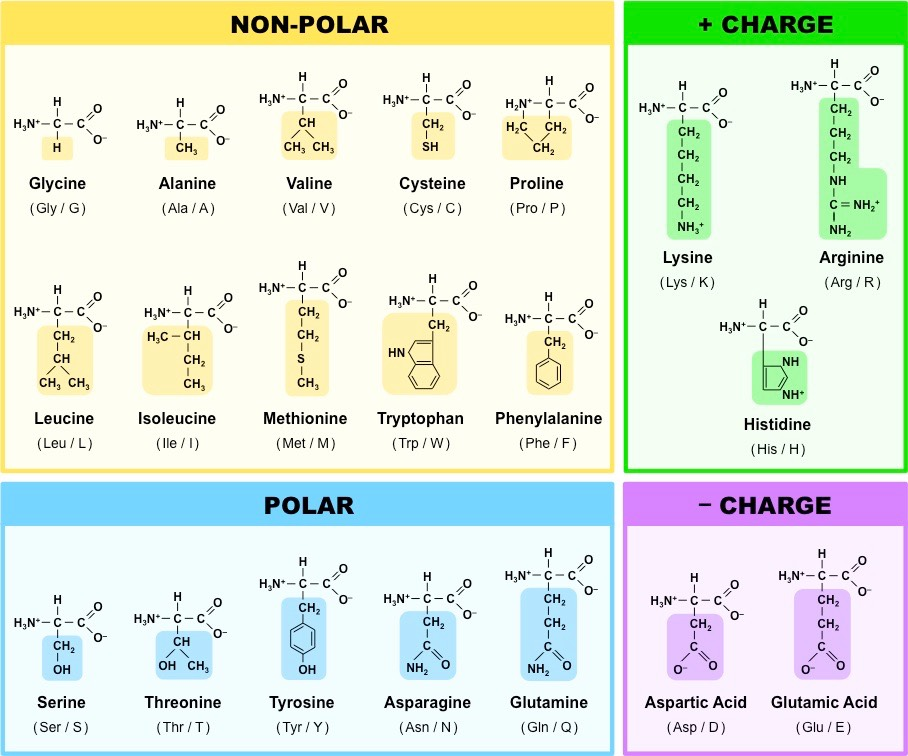
\includegraphics[width=0.85\textwidth]{ak.jpeg}
    \centering
    \label{}
\end{figure}


\begin{itemize}[nosep]
    \item dva cysteiny spolu tvoří sulfidický můstek
    \item všechny proteiny (alespoň hned po translaci) začínají na Met, u bakterií je to N-formylmethionin
    \item AK mo­hou být mod­i­fikovány (oligosacharidy, sul­fa­ti­zace, es­ter­i­fikace, fos­fory­lace, ami­dace, atd.)
    \item průměrná hmot­nost AA je 110g/mol
    \item existuje i několik vzácných AK
\begin{itemize}[nosep]
    \item selenocystein, pyrrolysin, N-formylmethionin
    \item jsou kódovány STOP kodony
\end{itemize}

\end{itemize}



\subsection{Disociace AK} \label{Disociace AK}


Měříme poměr koncentrací nedisociovaných a disociovaných kyselin.
\[\ce{HA <=> A^- + H^+} \\ K_a = \frac{[\ce{H^+}][\ce{A^-}]}{[\ce{HA}]},\]
kde \(K_a\) je takzvaná \emph{disociační konstanta}. Pokud přidáme nějakou kyselinu do vody, pH se časem ustálí na \(\text{pK}_a\) kyseliny.

\begin{figure}
    \caption{Prezentace č. 1, slide č. 23}
    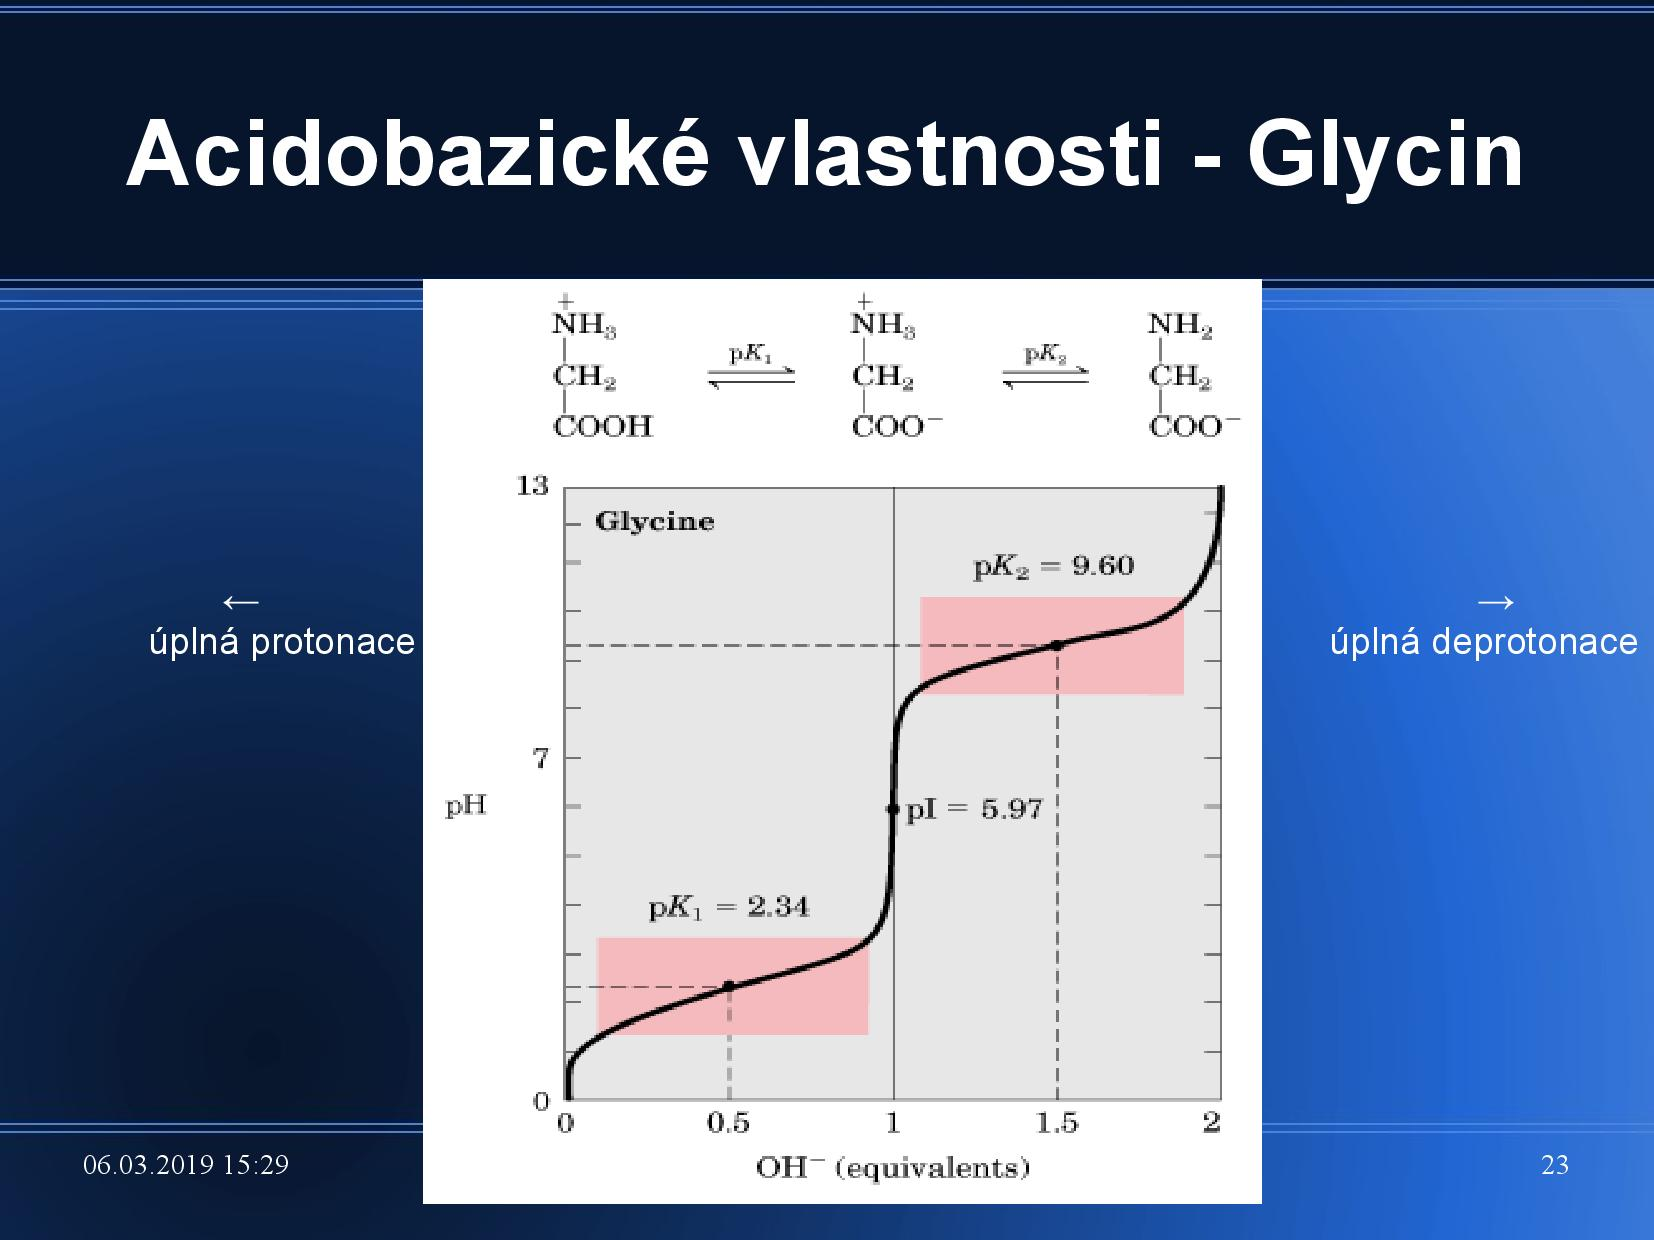
\includegraphics[width=0.85\textwidth]{slides-1/slide-23.jpg}
    \centering
    \label{slides-1-slide-23}
\end{figure}
\begin{figure}
    \caption{Prezentace č. 1, slide č. 26}
    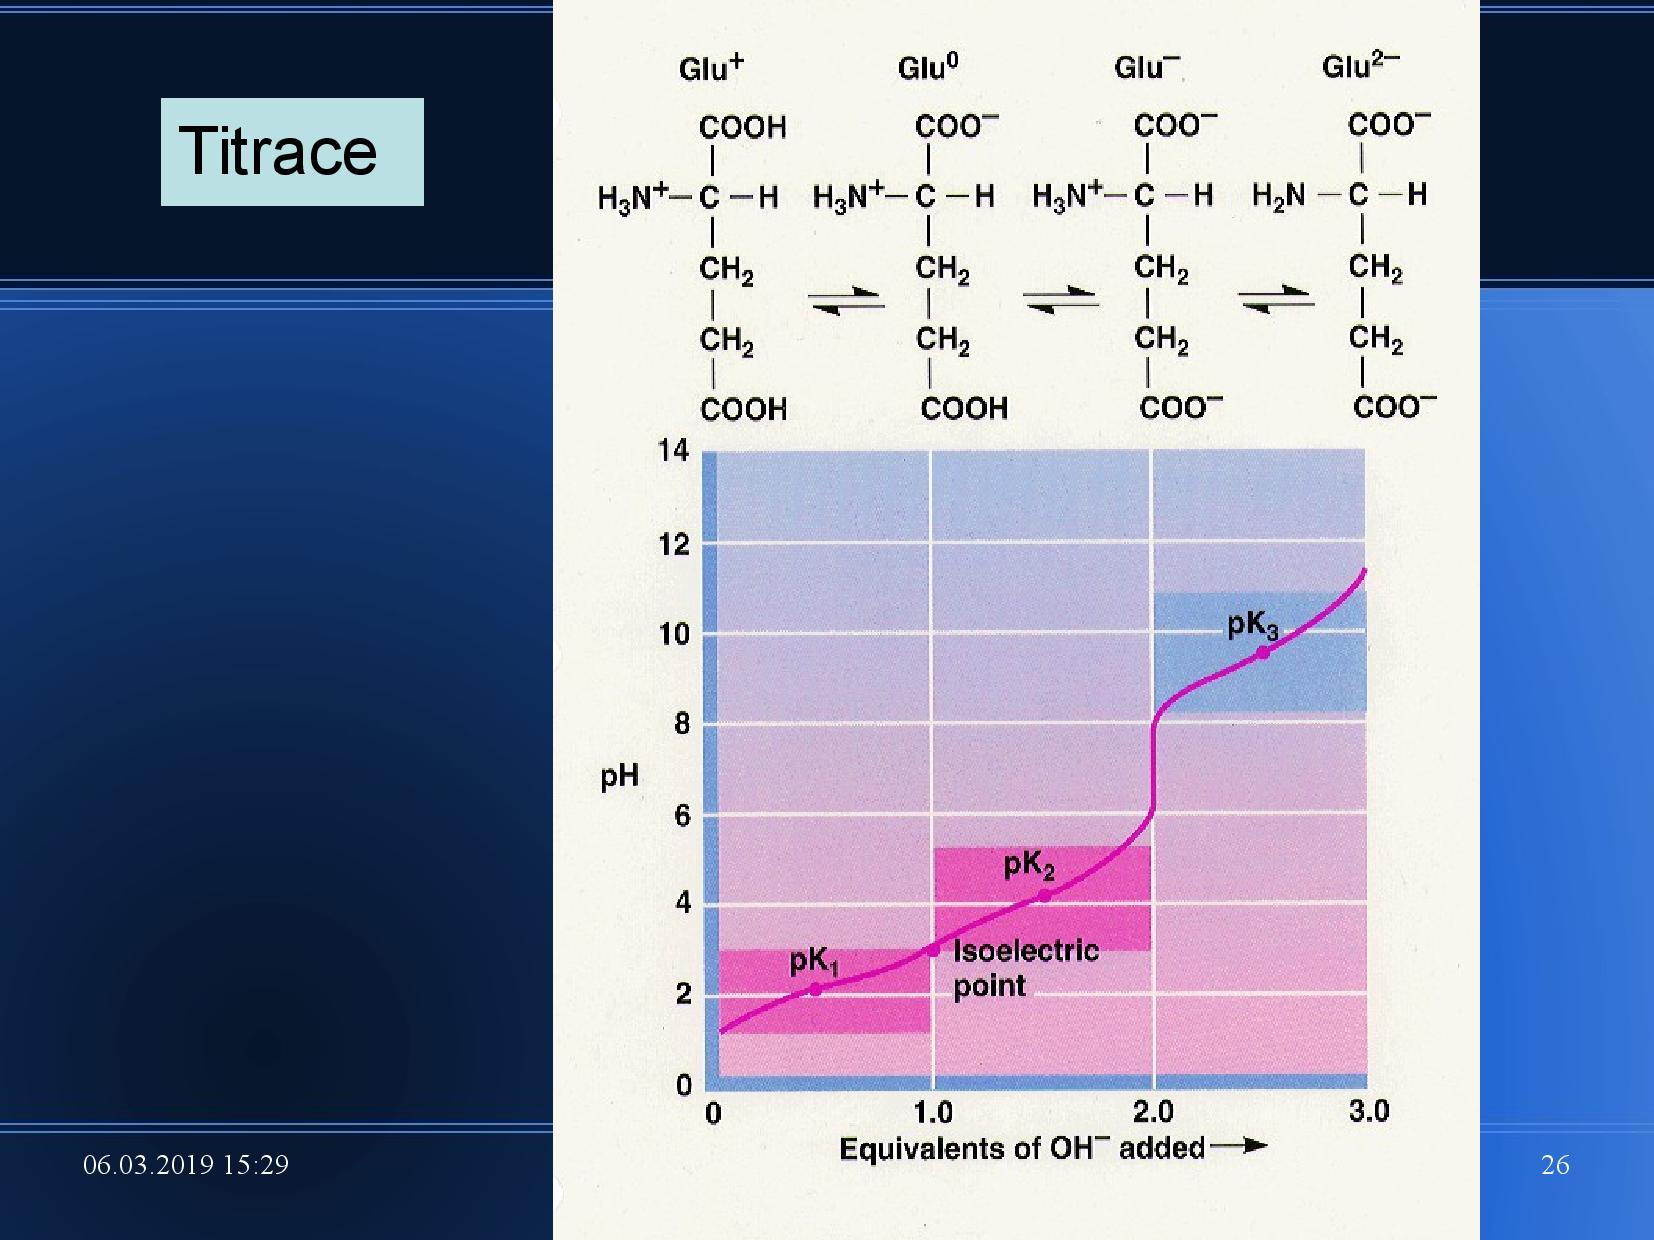
\includegraphics[width=0.85\textwidth]{slides-1/slide-26.jpg}
    \centering
    \label{slides-1-slide-26}
\end{figure}

Definujeme také \emph{izoelektrický bod} AK, což je bod, kdy kyselina nemá žádný náboj. Počítá se jako průměr jednotlivých \(\text{pK}_a\) všech možných forem AK, podle toho, který z vodíků je odštěpený. Pro vodík v \(\ce{COOH}\) je \(\text{pK}_a \approx 2\), pro ten v \(\ce{NH3}\) \(\text{pK}_a \approx 10\).

\subsection{Další vlastnosti AK} \label{Další vlastnosti AK}


\begin{figure}
    \caption{Prezentace č. 1, slide č. 32}
    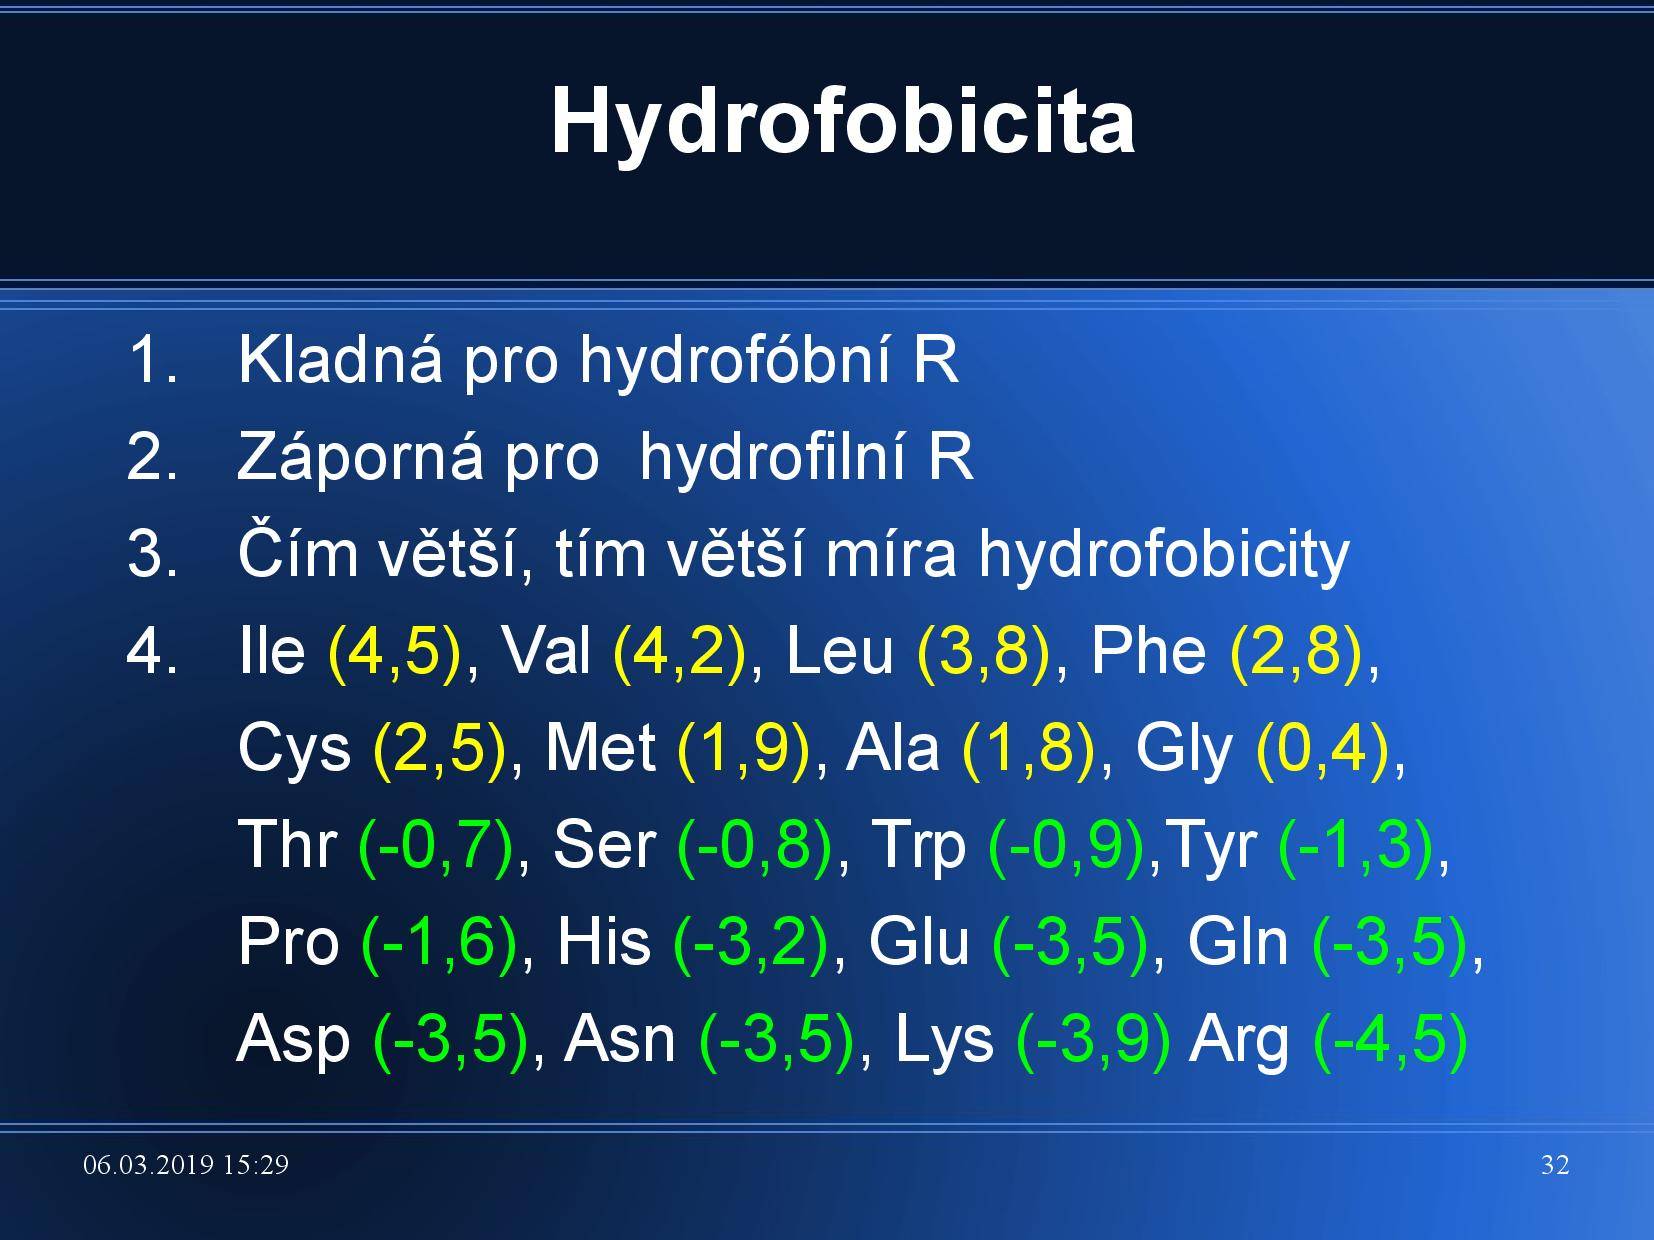
\includegraphics[width=0.85\textwidth]{slides-1/slide-32.jpg}
    \centering
    \label{slides-1-slide-32}
\end{figure}

\textbf{Hydrofobicita} udává, jako moc je protein hydrofobní; značí se \(R\), a má kladné hodnoty pro hydrofobní proteiny.

\begin{figure}
    \caption{Prezentace č. 1, slide č. 33}
    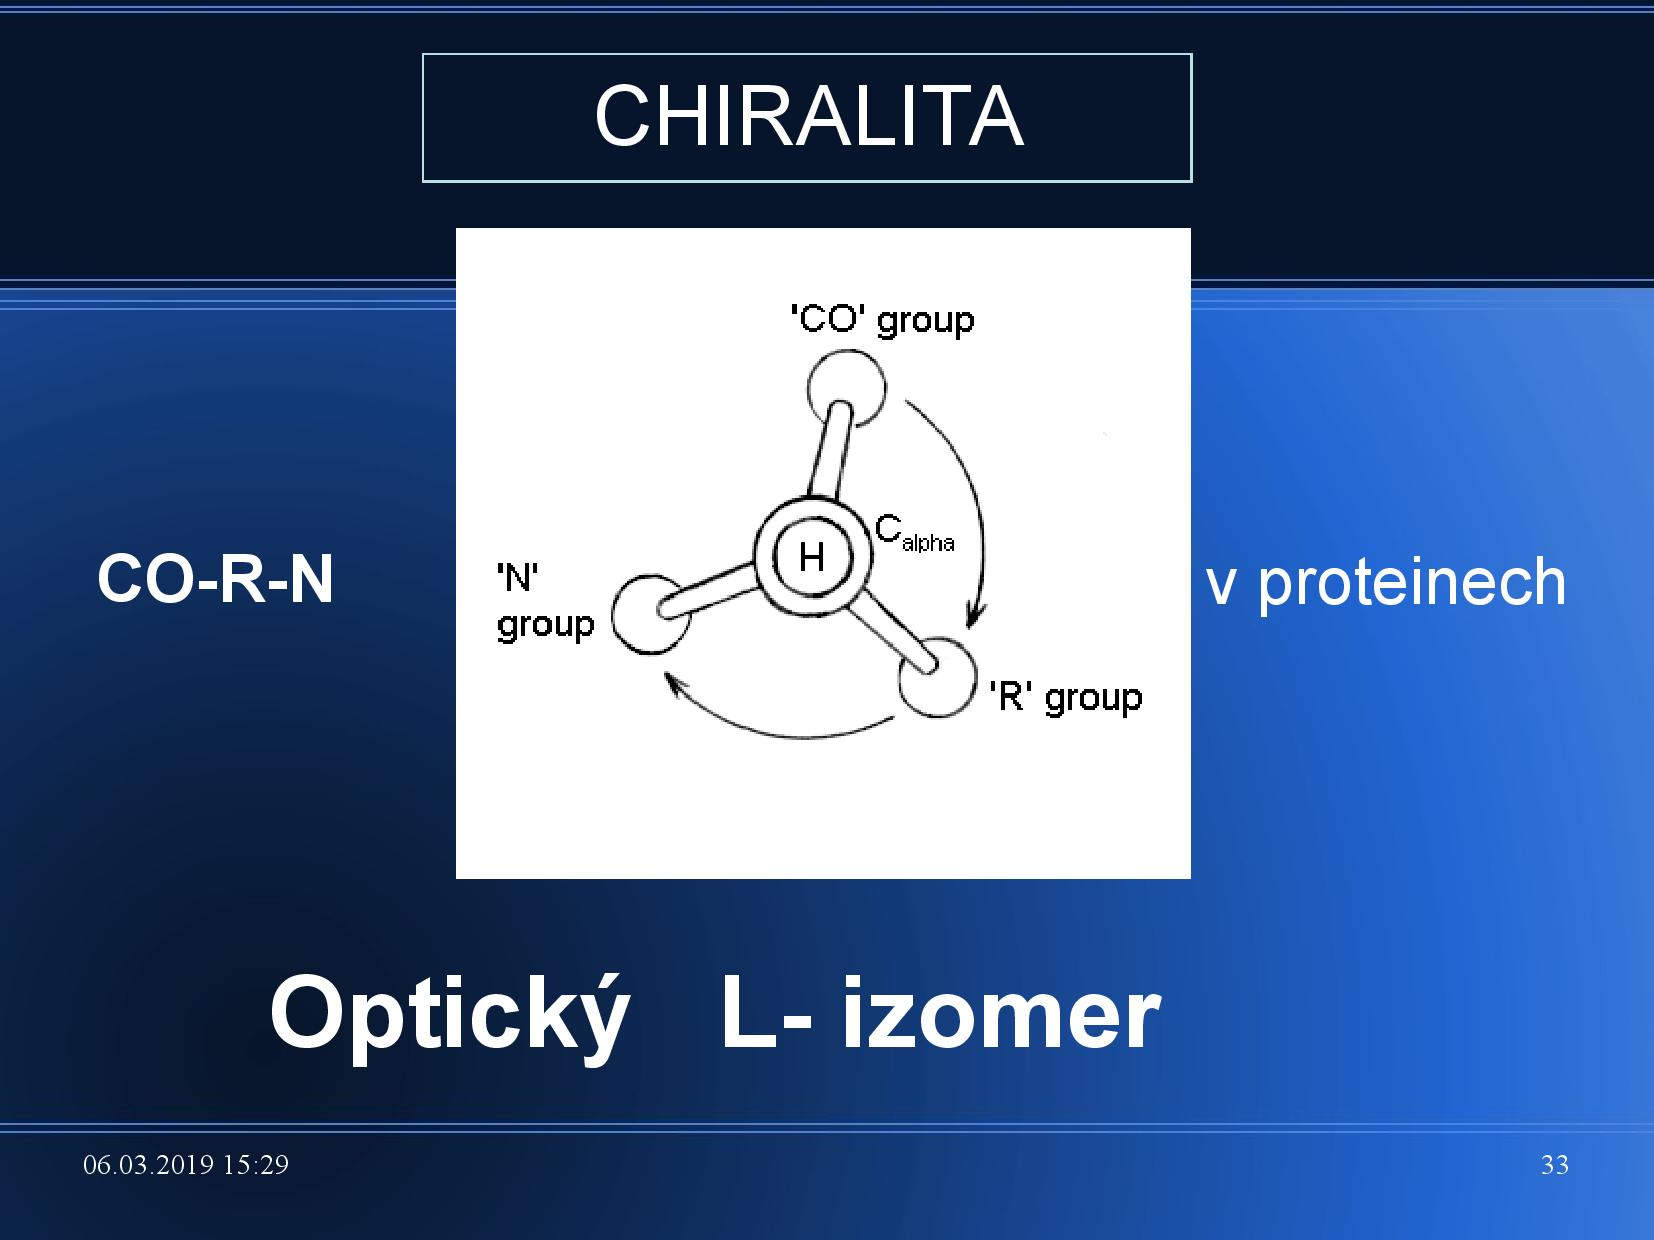
\includegraphics[width=0.85\textwidth]{slides-1/slide-33.jpg}
    \centering
    \label{slides-1-slide-33}
\end{figure}

\paragraph{Chiralita}
\begin{itemize}[nosep]
    \item z uhlíku vychází čtyři různé substituenty
    \item u AK je jím \(\ce{C\alpha}\)
    \item rozlišení optických L a D izomerů
\begin{itemize}[nosep]
    \item L-izomer: pokud H míří k nám, COOH nahoru, potom po směru hodinových ručiček: \textbf{CO-R-N}
    \item optické izomery pootáčejí rovinu polarizovaného světla
    \item L/D izomery nestáčí tuto rovinu nutně vždy na stejnou stranu
\end{itemize}

    \item většina přírodních AK jsou L-izomery (vyjímky například buněčné stěny bakterií)
    \item může se stát, že máme více chirálních uhlíků, poté existuje \(2^k\) forem molekuly
\end{itemize}



\section{Peptidová vazba} \label{Peptidová vazba}


\begin{figure}
    \caption{Prezentace č. 1, slide č. 44}
    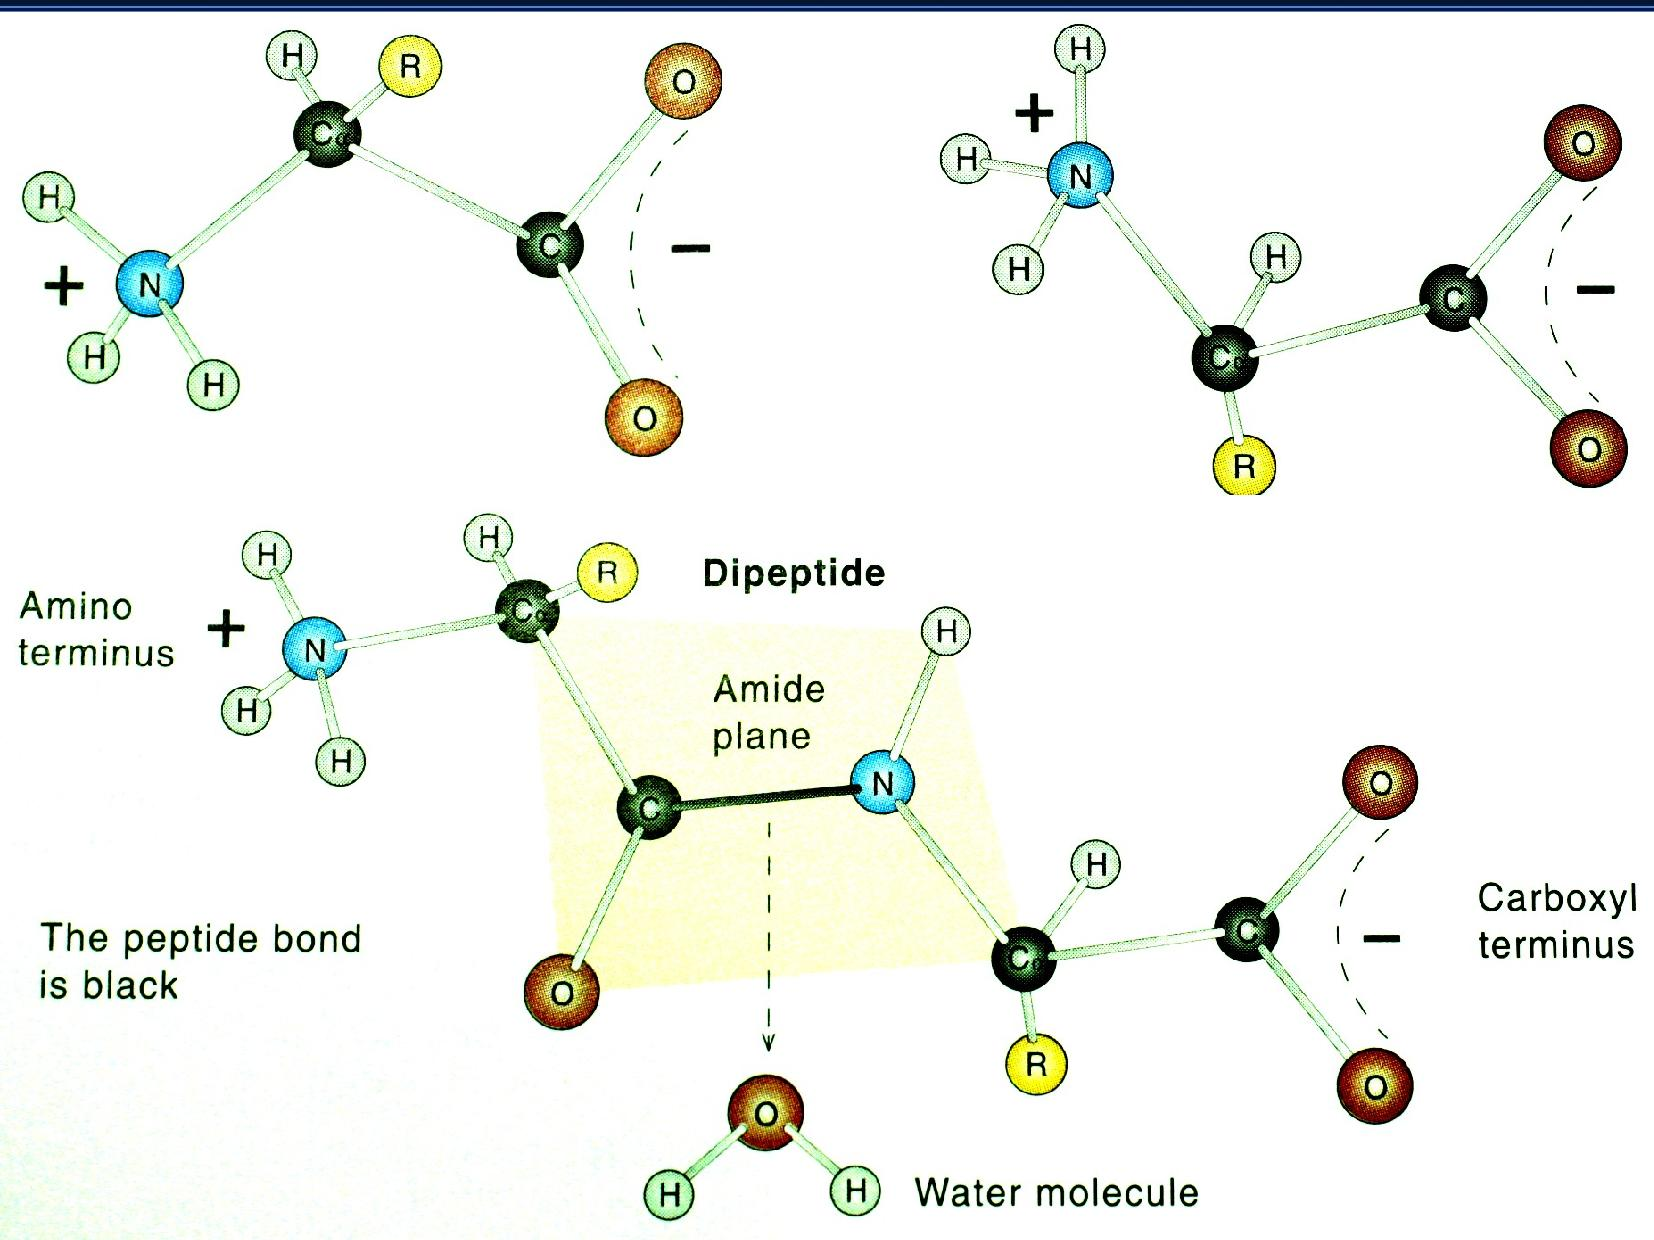
\includegraphics[width=0.85\textwidth]{slides-1/slide-44.jpg}
    \centering
    \label{slides-1-slide-44}
\end{figure}
\begin{figure}
    \caption{Prezentace č. 1, slide č. 45}
    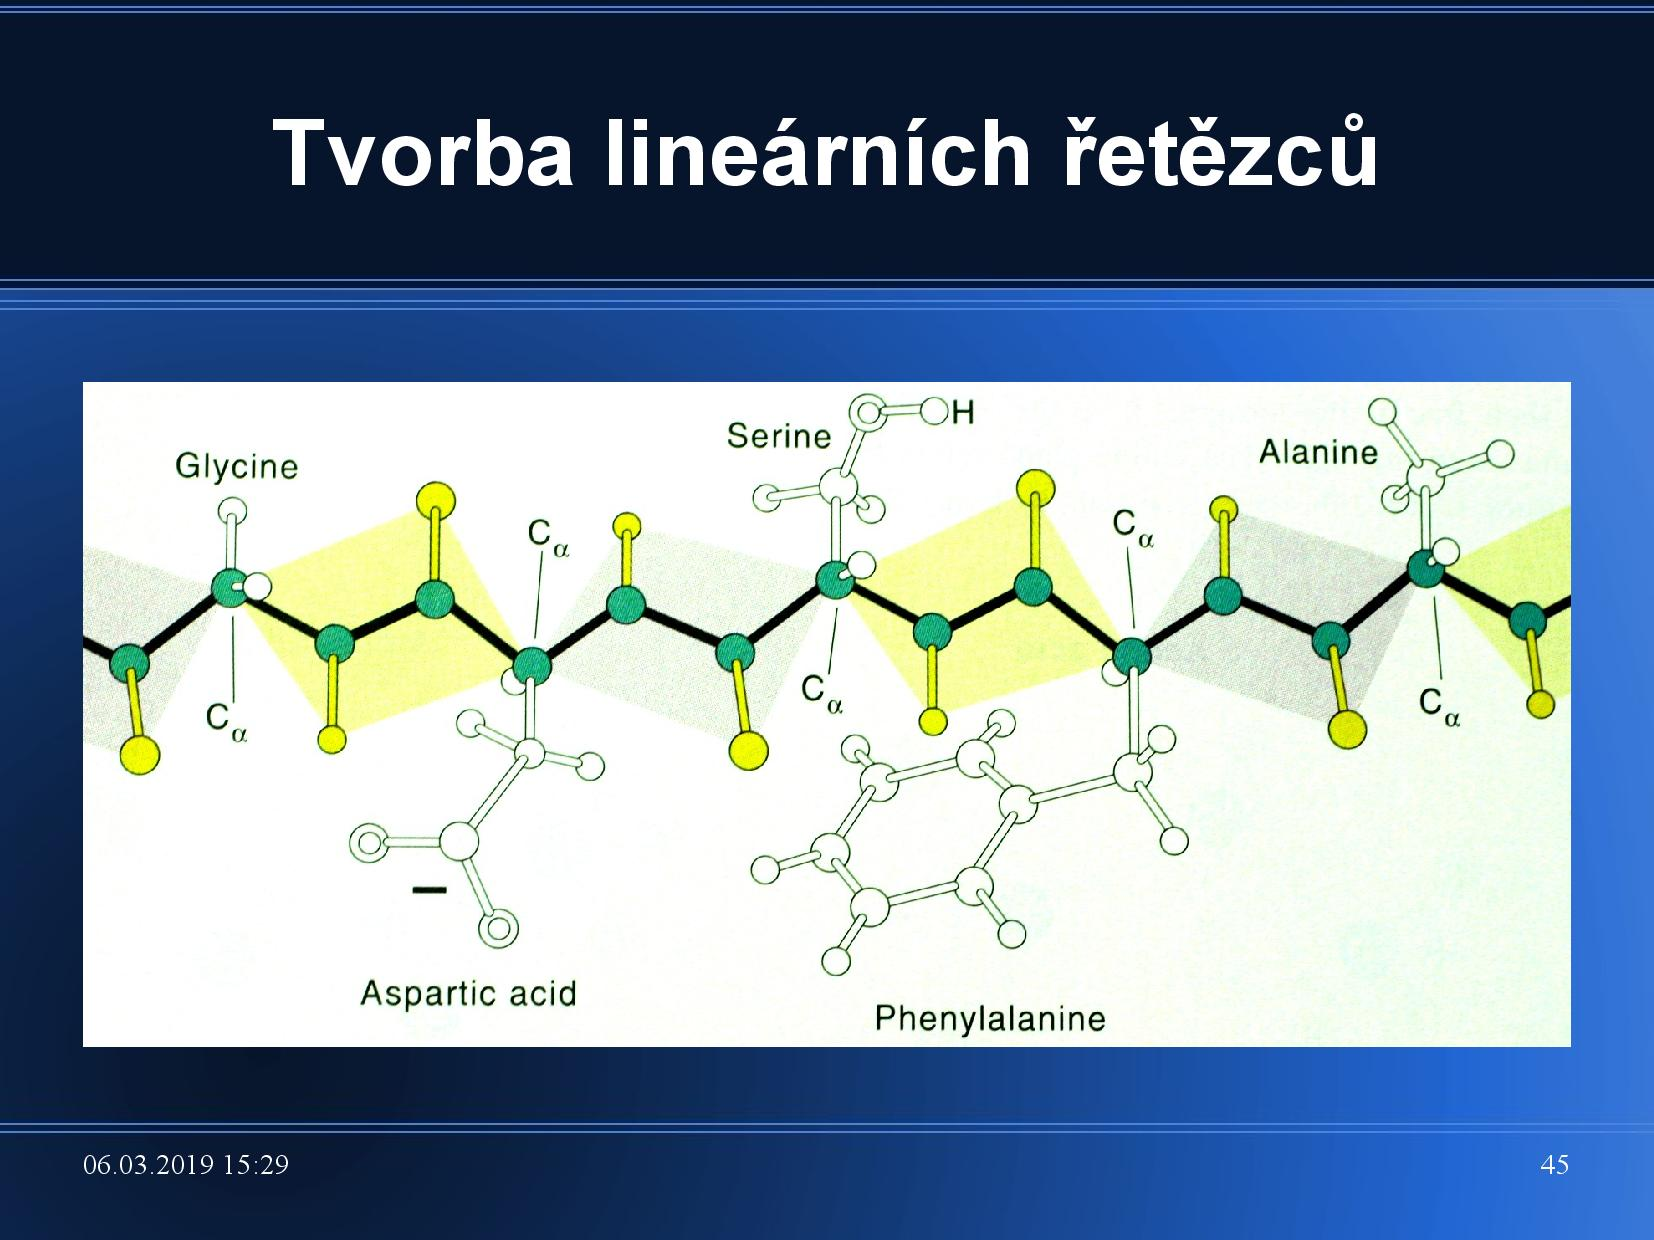
\includegraphics[width=0.85\textwidth]{slides-1/slide-45.jpg}
    \centering
    \label{slides-1-slide-45}
\end{figure}

Vazba mezi dvěma AK, které se účasntní původní \(\ce{COOH}\) a \(\ce{NH2}\) skupiny.

\begin{figure}
    \caption{Prezentace č. 1, slide č. 46}
    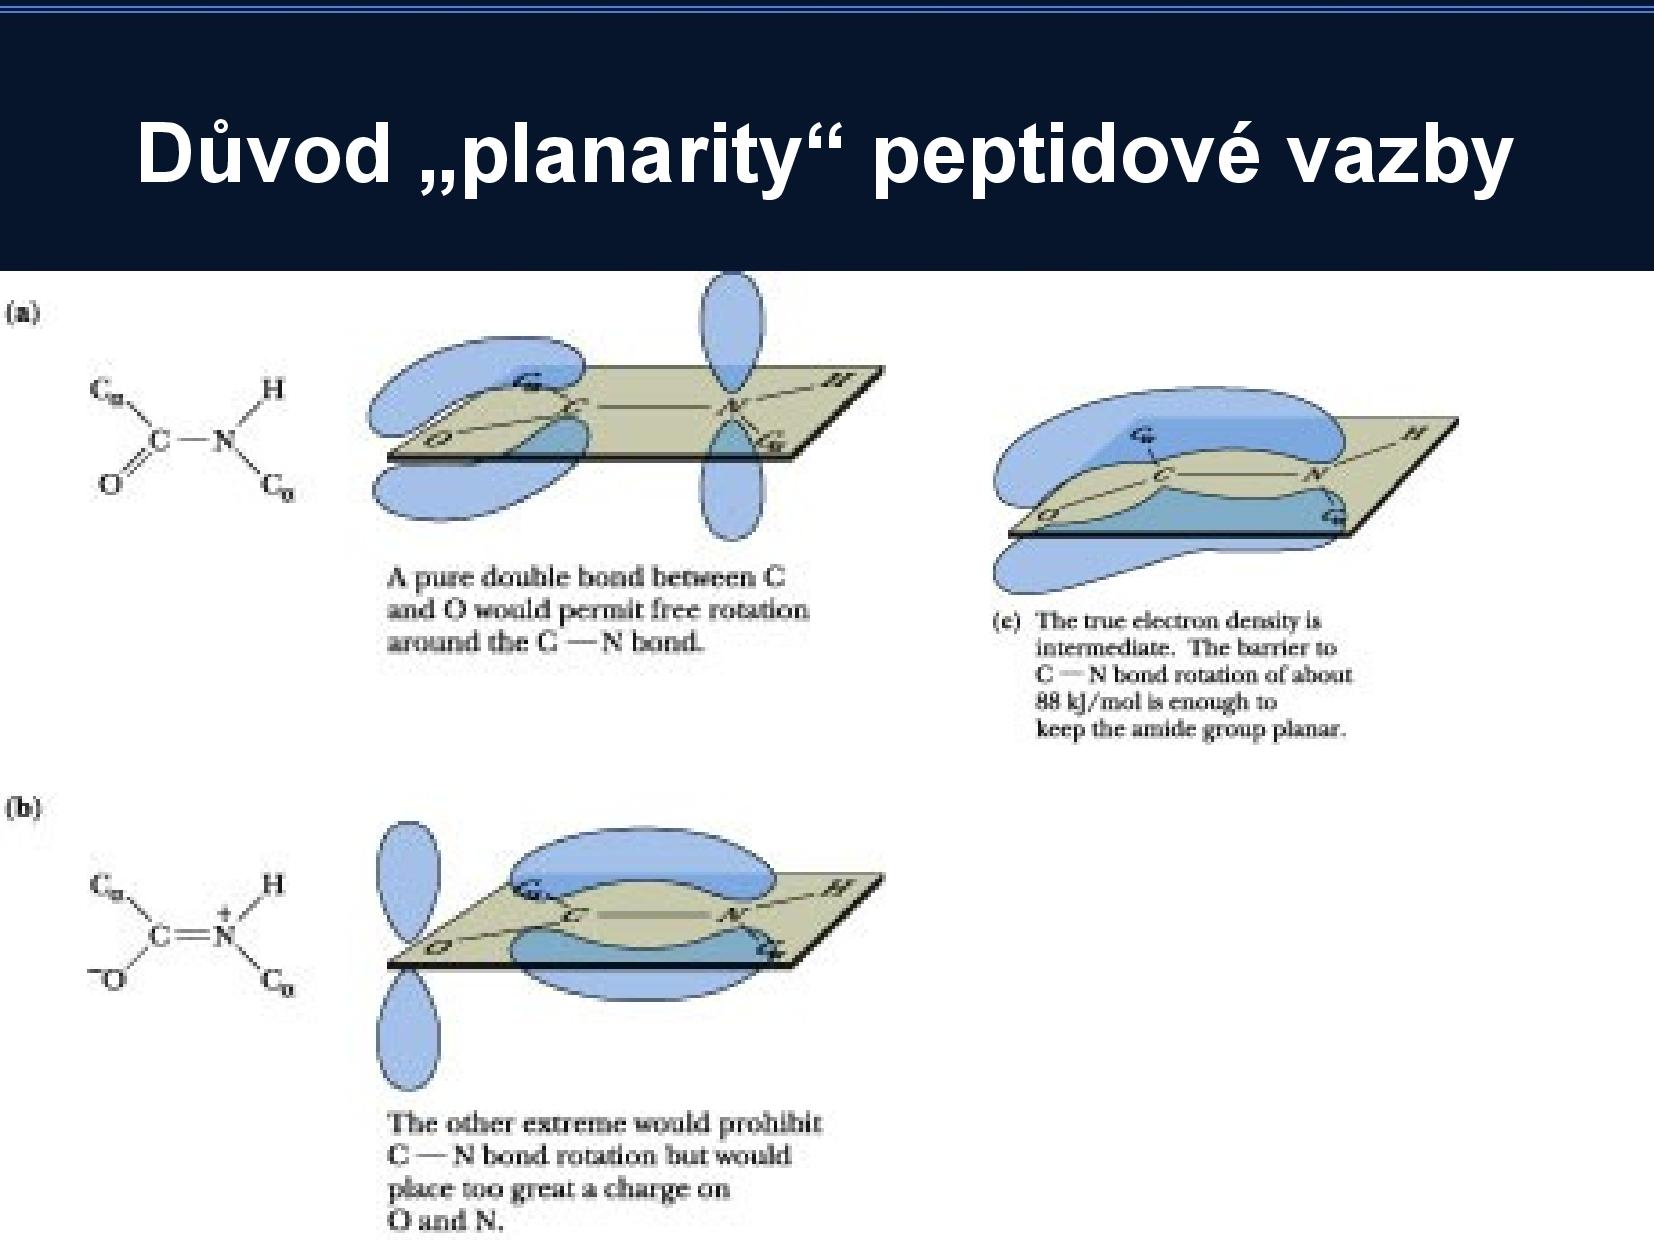
\includegraphics[width=0.85\textwidth]{slides-1/slide-46.jpg}
    \centering
    \label{slides-1-slide-46}
\end{figure}

Vazba je planární, protože dvojná vazba \(\ce{C=O}\) někdy přejde na vazbu \(\ce{C-N}\) (tzv. \emph{mezomernie}). Rotace je tedy možná pouze v "rozích" vazby, kolem vazeb vycházejících z \(\ce{C\alpha}\).

\begin{figure}
    \caption{Prezentace č. 1, slide č. 50}
    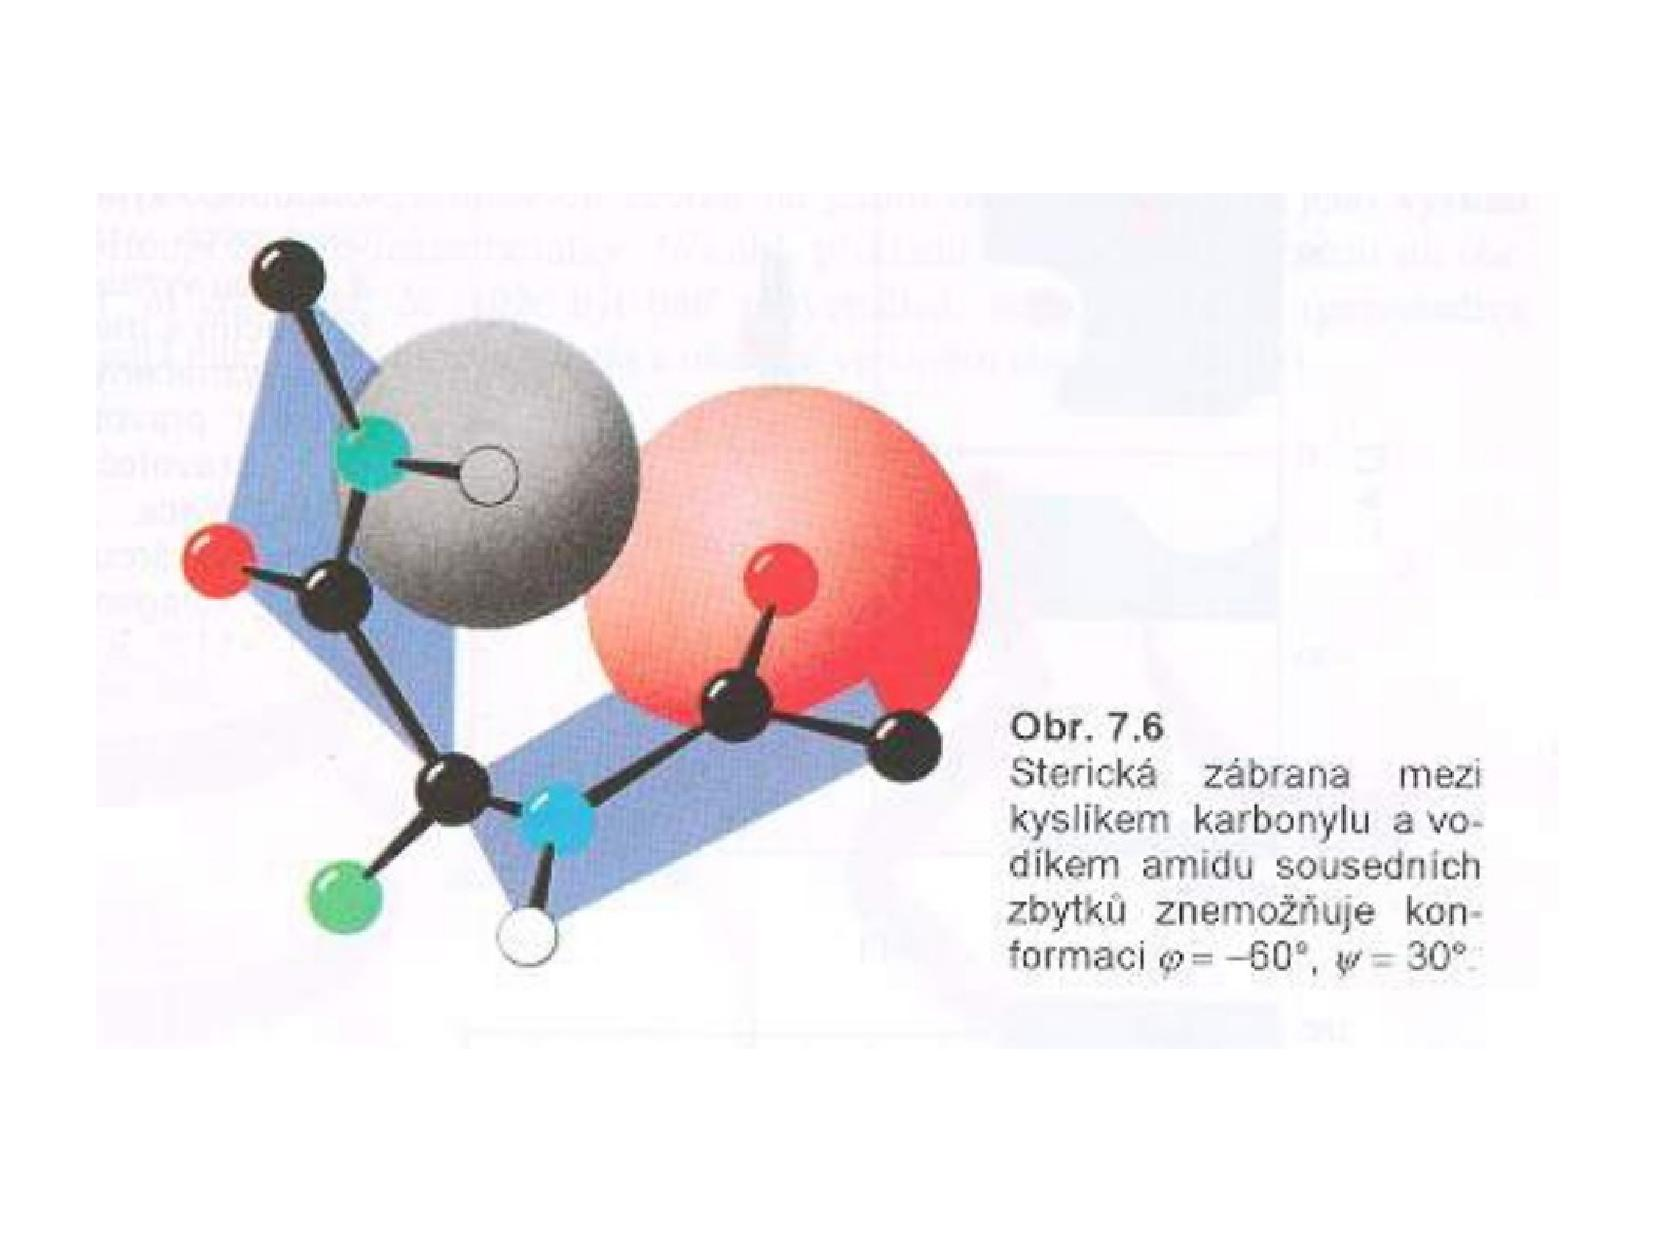
\includegraphics[width=0.85\textwidth]{slides-1/slide-50.jpg}
    \centering
    \label{slides-1-slide-50}
\end{figure}
\begin{figure}
    \caption{Prezentace č. 1, slide č. 51}
    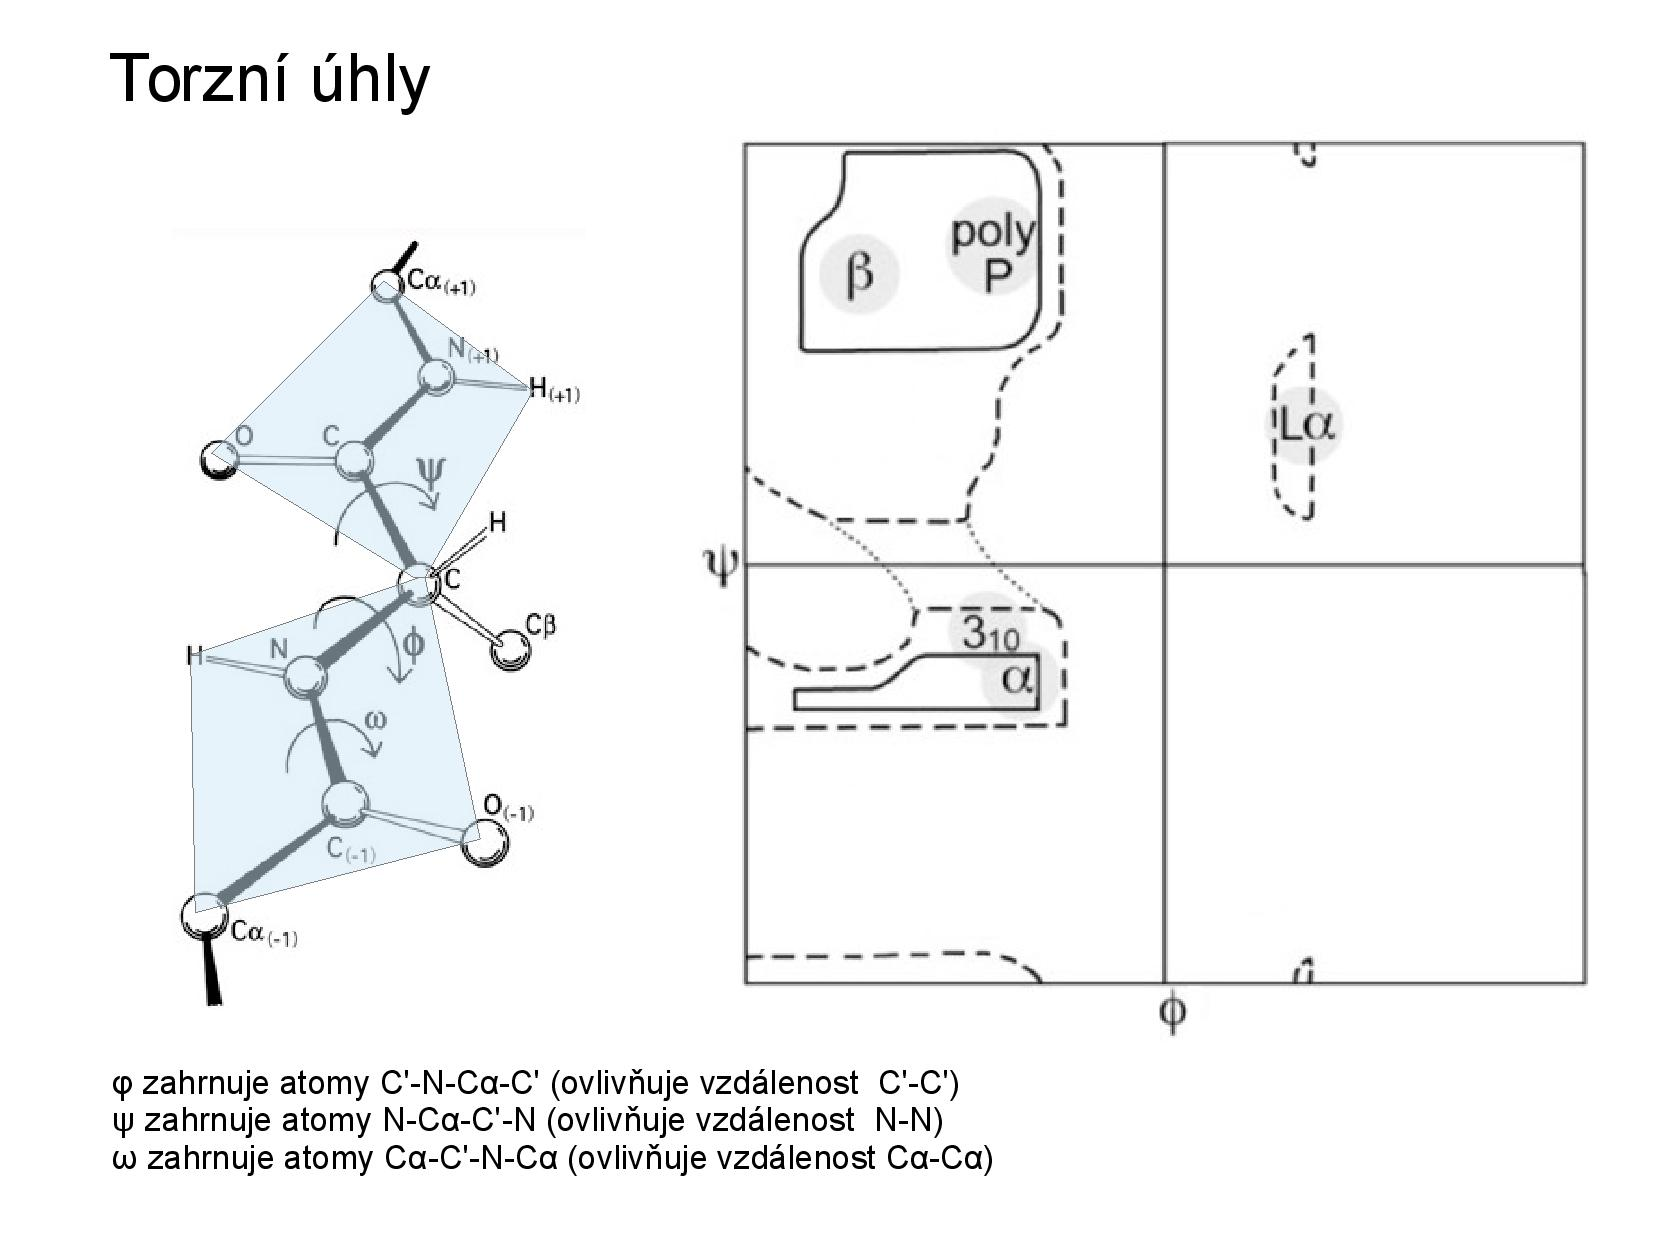
\includegraphics[width=0.85\textwidth]{slides-1/slide-51.jpg}
    \centering
    \label{slides-1-slide-51}
\end{figure}
\begin{figure}
    \caption{Prezentace č. 1, slide č. 52}
    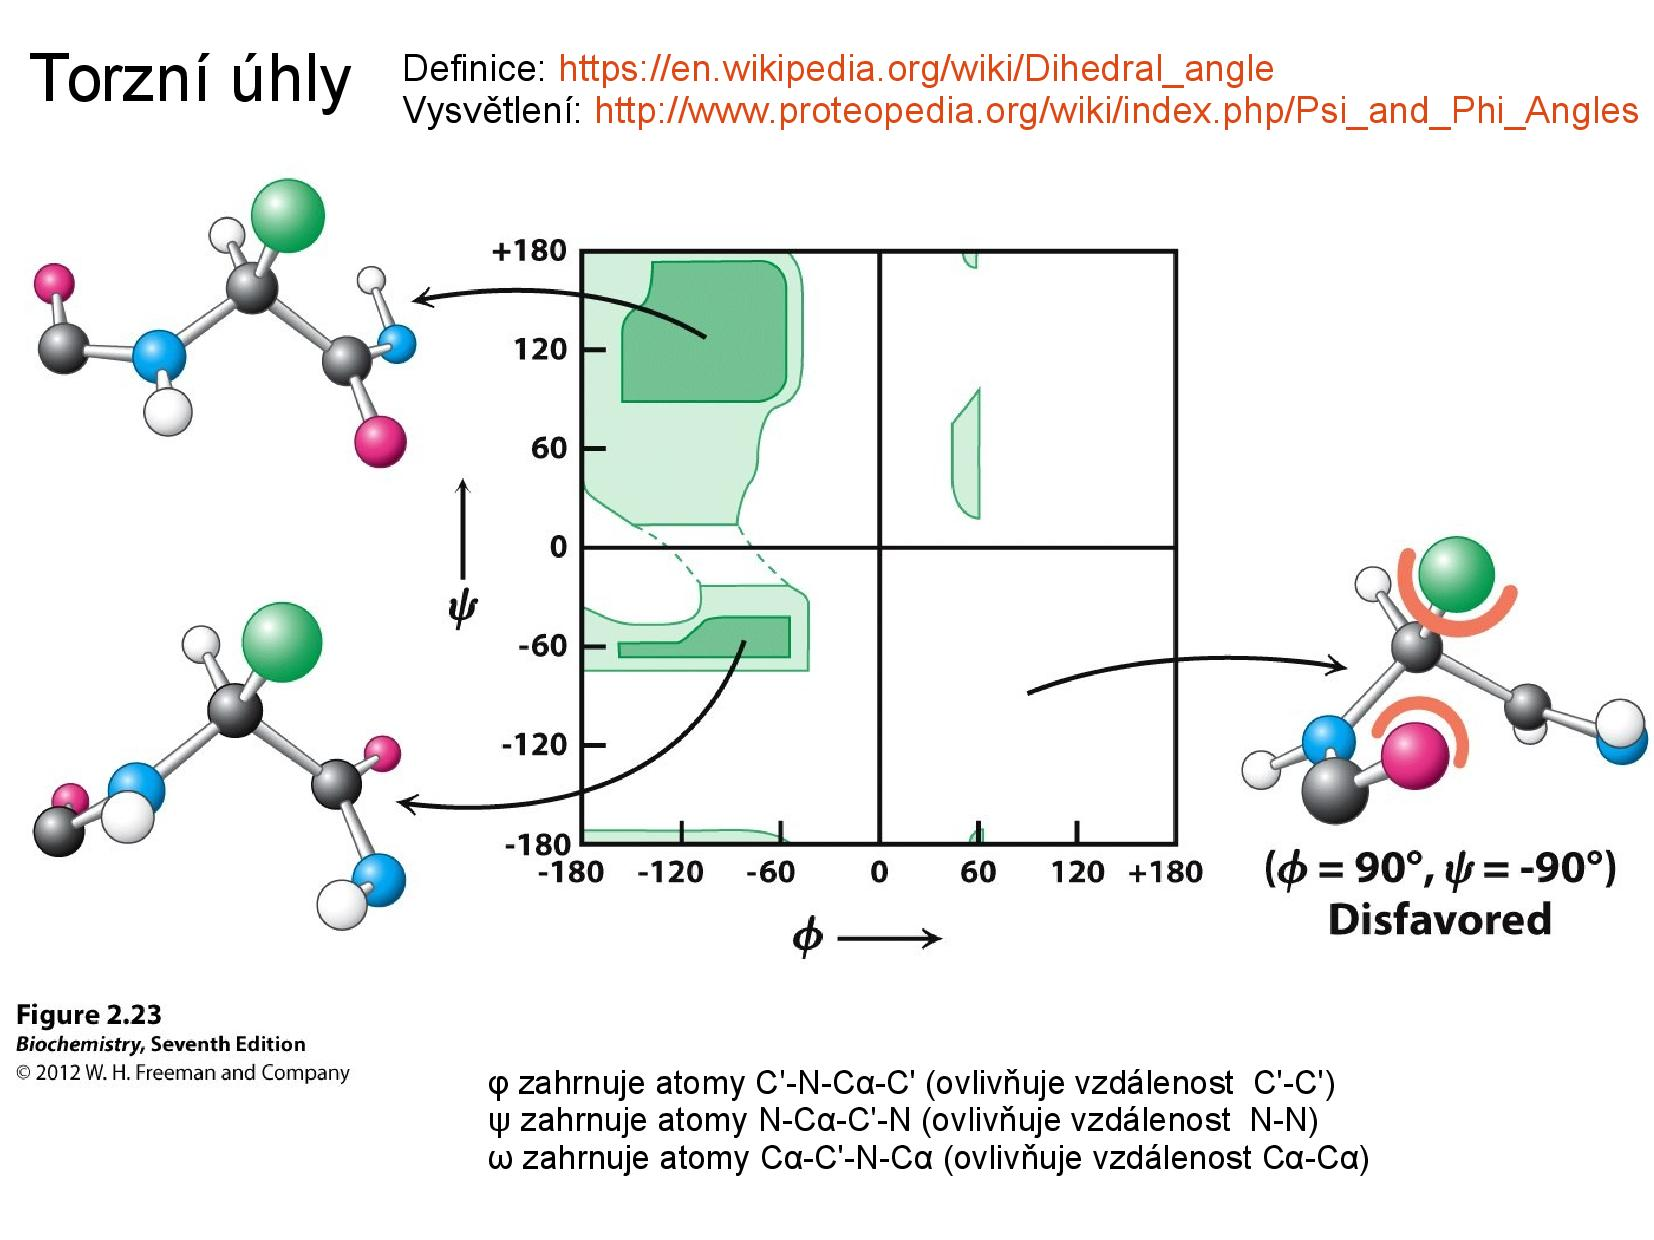
\includegraphics[width=0.85\textwidth]{slides-1/slide-52.jpg}
    \centering
    \label{slides-1-slide-52}
\end{figure}

\paragraph{Torzní úhly}
\begin{itemize}[nosep]
    \item rotace kolem \(\ce{C\alpha}\) jsou možné, ale kyslík a vodík si při určitých hodnotách rotace překážejí
    \item jsou povolené dvě konformace: \textbf{cis} a \textbf{trans}
\begin{itemize}[nosep]
    \item zpravidla u všech proteinů se vyskytuje konformace trans
    \item cis konformace jen výjimenčně u prolinu
\end{itemize}

    \item torzní úhly: \(\varphi\) značí úhel \(\ce{C-N}\), \(\psi\) značí úhel \(\ce{C-C}\)
\begin{itemize}[nosep]
    \item povolené hodnoty těchto úhlů můžeme zanést do tzv. \emph{Ramachandranova grafu}
    \item v Ramachandranově grafu nejprve vypíšeme oblasti pravděpodobných hodnot, teoreticky možných hodnot a nepravděpodobných hodnot, poté srovnáma naměřená data s těmito zónami
    \item určité oblasti odpovídají určitým sekundárním strukturů, viz slide \begin{figure}
    \caption{Prezentace č. 1, slide č. 53}
    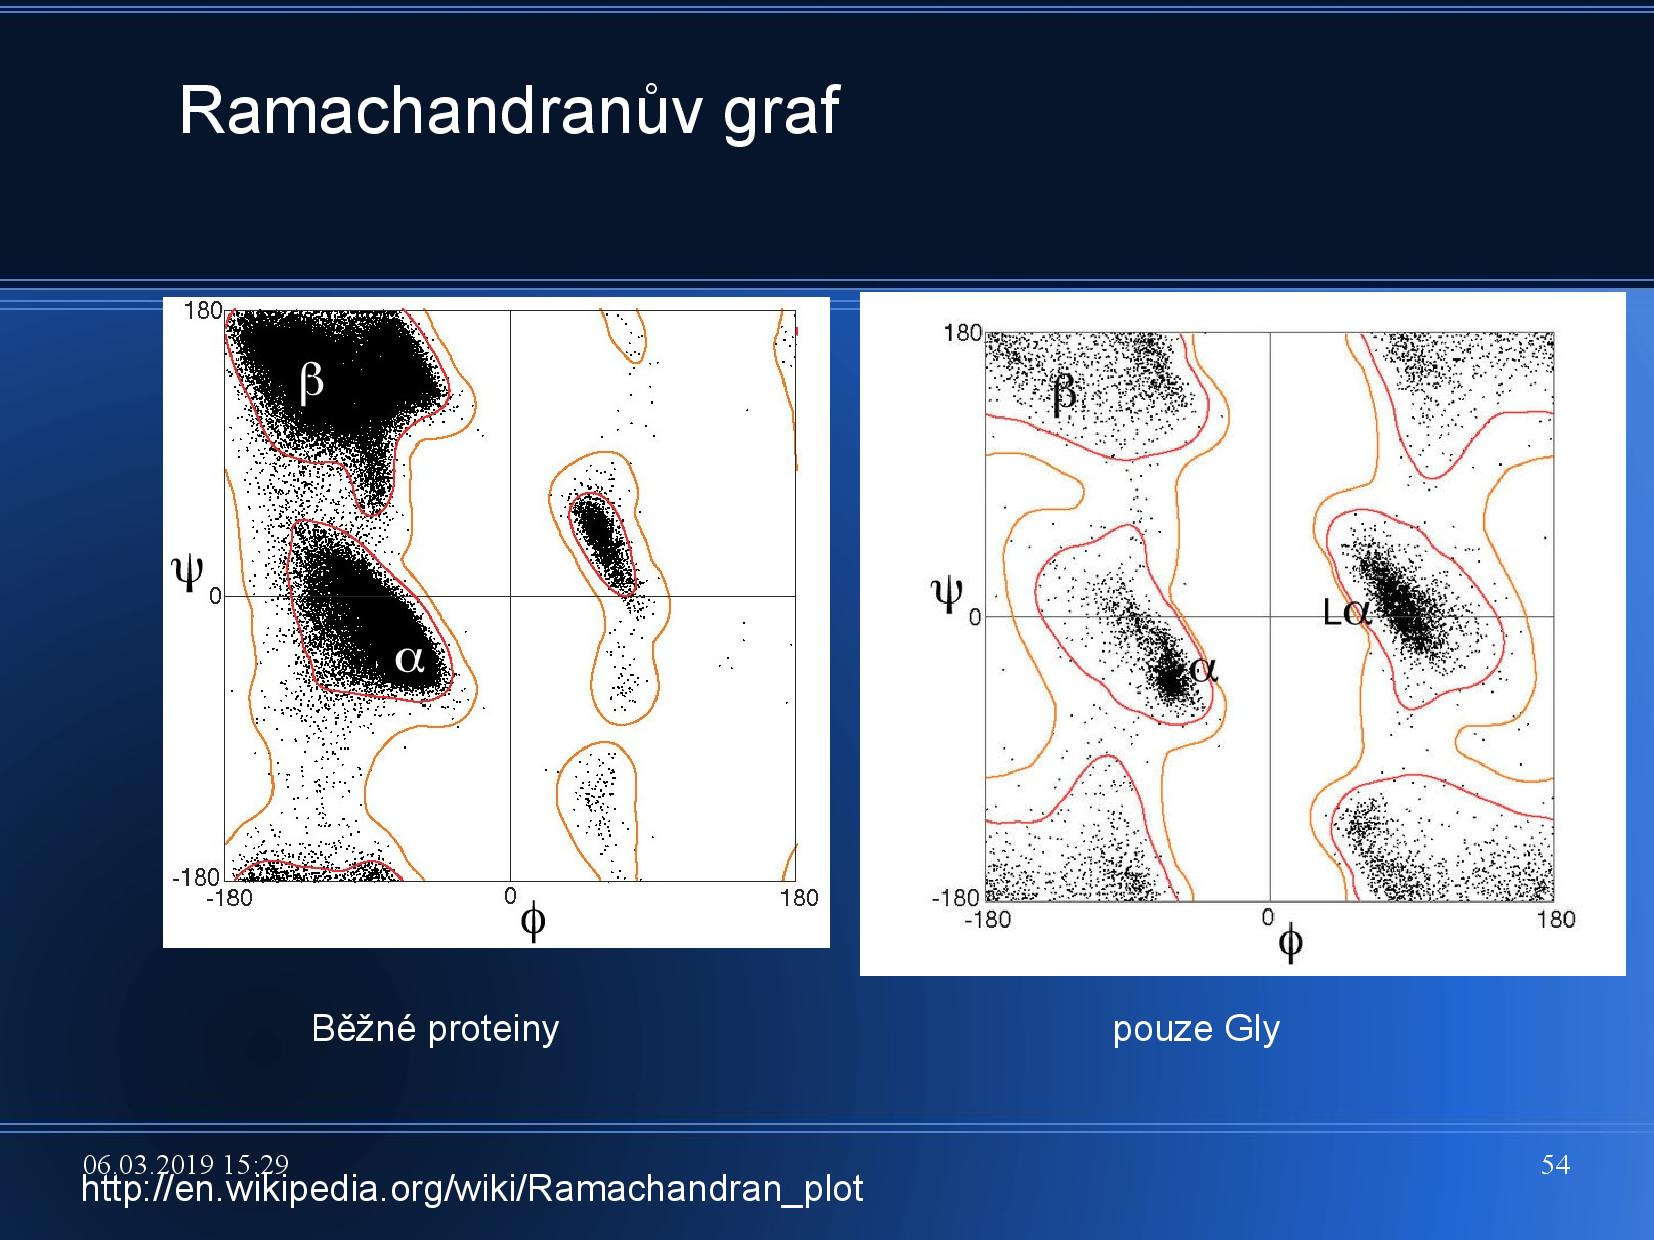
\includegraphics[width=0.85\textwidth]{slides-1/slide-53.jpg}
    \centering
    \label{slides-1-slide-53}
\end{figure}

\end{itemize}

\end{itemize}



\section{Sekundární struktury} \label{Sekundární struktury}


\begin{figure}
    \caption{Prezentace č. 1, slide č. 57}
    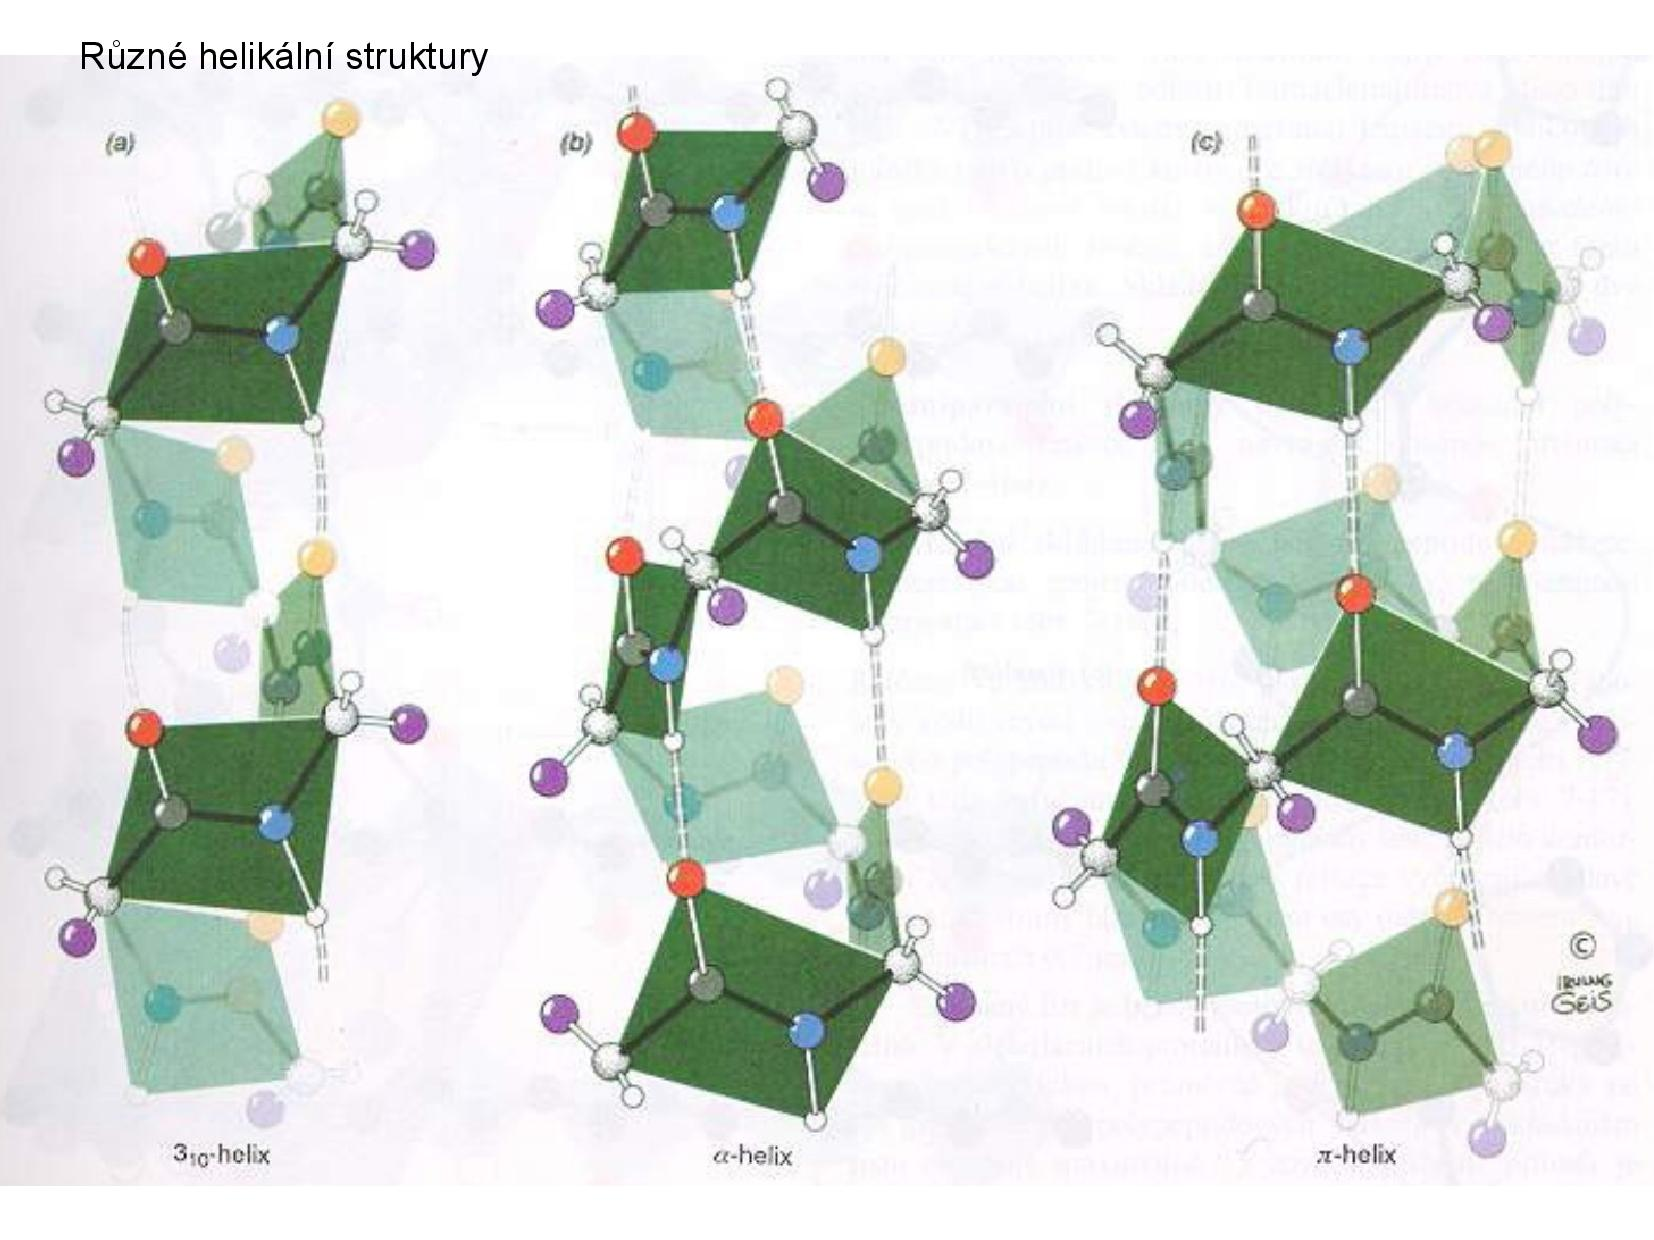
\includegraphics[width=0.85\textwidth]{slides-1/slide-57.jpg}
    \centering
    \label{slides-1-slide-57}
\end{figure}

\paragraph{Helikální}
\begin{itemize}[nosep]
    \item \(\alpha\) helix
\begin{itemize}[nosep]
    \item pravotočivá šroubovice
    \item stabilizován vodíkovými můstky mezi vodíkem aminoskupiny a kyslíkem karbonylu
    \item vzálenost vodíkových můstků je 4AK
    \item 3,6 AK na otáčku
    \item upostřed není dutina
    \item postranní řetězce vždy směřují ven
\end{itemize}

    \item \(3_{10}\) helix
\begin{itemize}[nosep]
    \item interakce mezi první a třetí AK
    \item vzácnejší, vyskytuje se na okrajích sekundárních struktur
\end{itemize}

    \item \(\pi\) helix
\begin{itemize}[nosep]
    \item interakce mezi první a pátou AK
    \item vzácnejší, vyskytuje se na okrajích sekundárních struktur
\end{itemize}

\end{itemize}



\begin{figure}
    \caption{Prezentace č. 1, slide č. 56}
    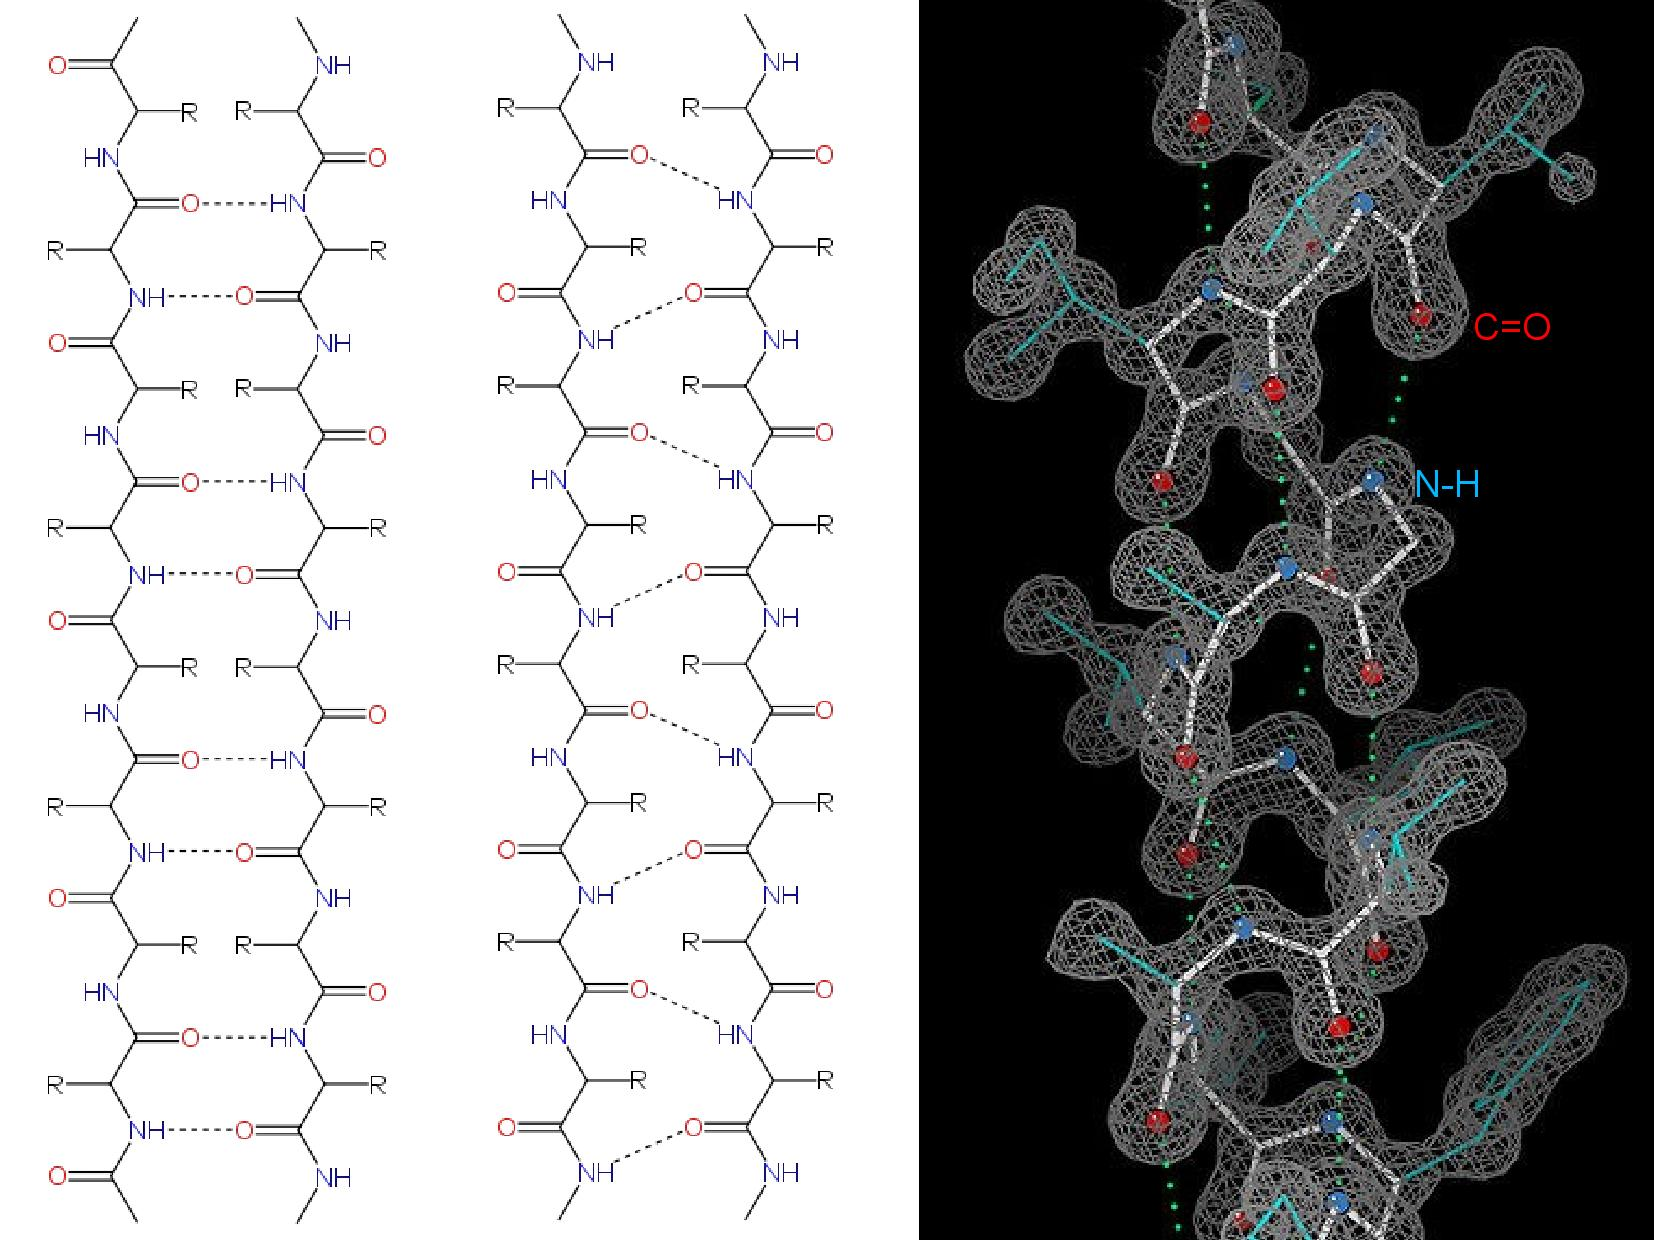
\includegraphics[width=0.85\textwidth]{slides-1/slide-56.jpg}
    \centering
    \label{slides-1-slide-56}
\end{figure}

\paragraph{Beta struktury}
\begin{itemize}[nosep]
    \item interaguje opět vodík na aminoskupině s karbonylem, ale mohou být v rámci řetězce i daleko od sebe
    \item paralelní a antiparalelní (ten je stabilnější)
\end{itemize}



\chapter{Metody pozorování proteinů} \label{Metody pozorování proteinů}


\section{Spektrofotometrie} \label{Spektrofotometrie}


\begin{figure}
    \caption{Prezentace č. 2, slide č. 27}
    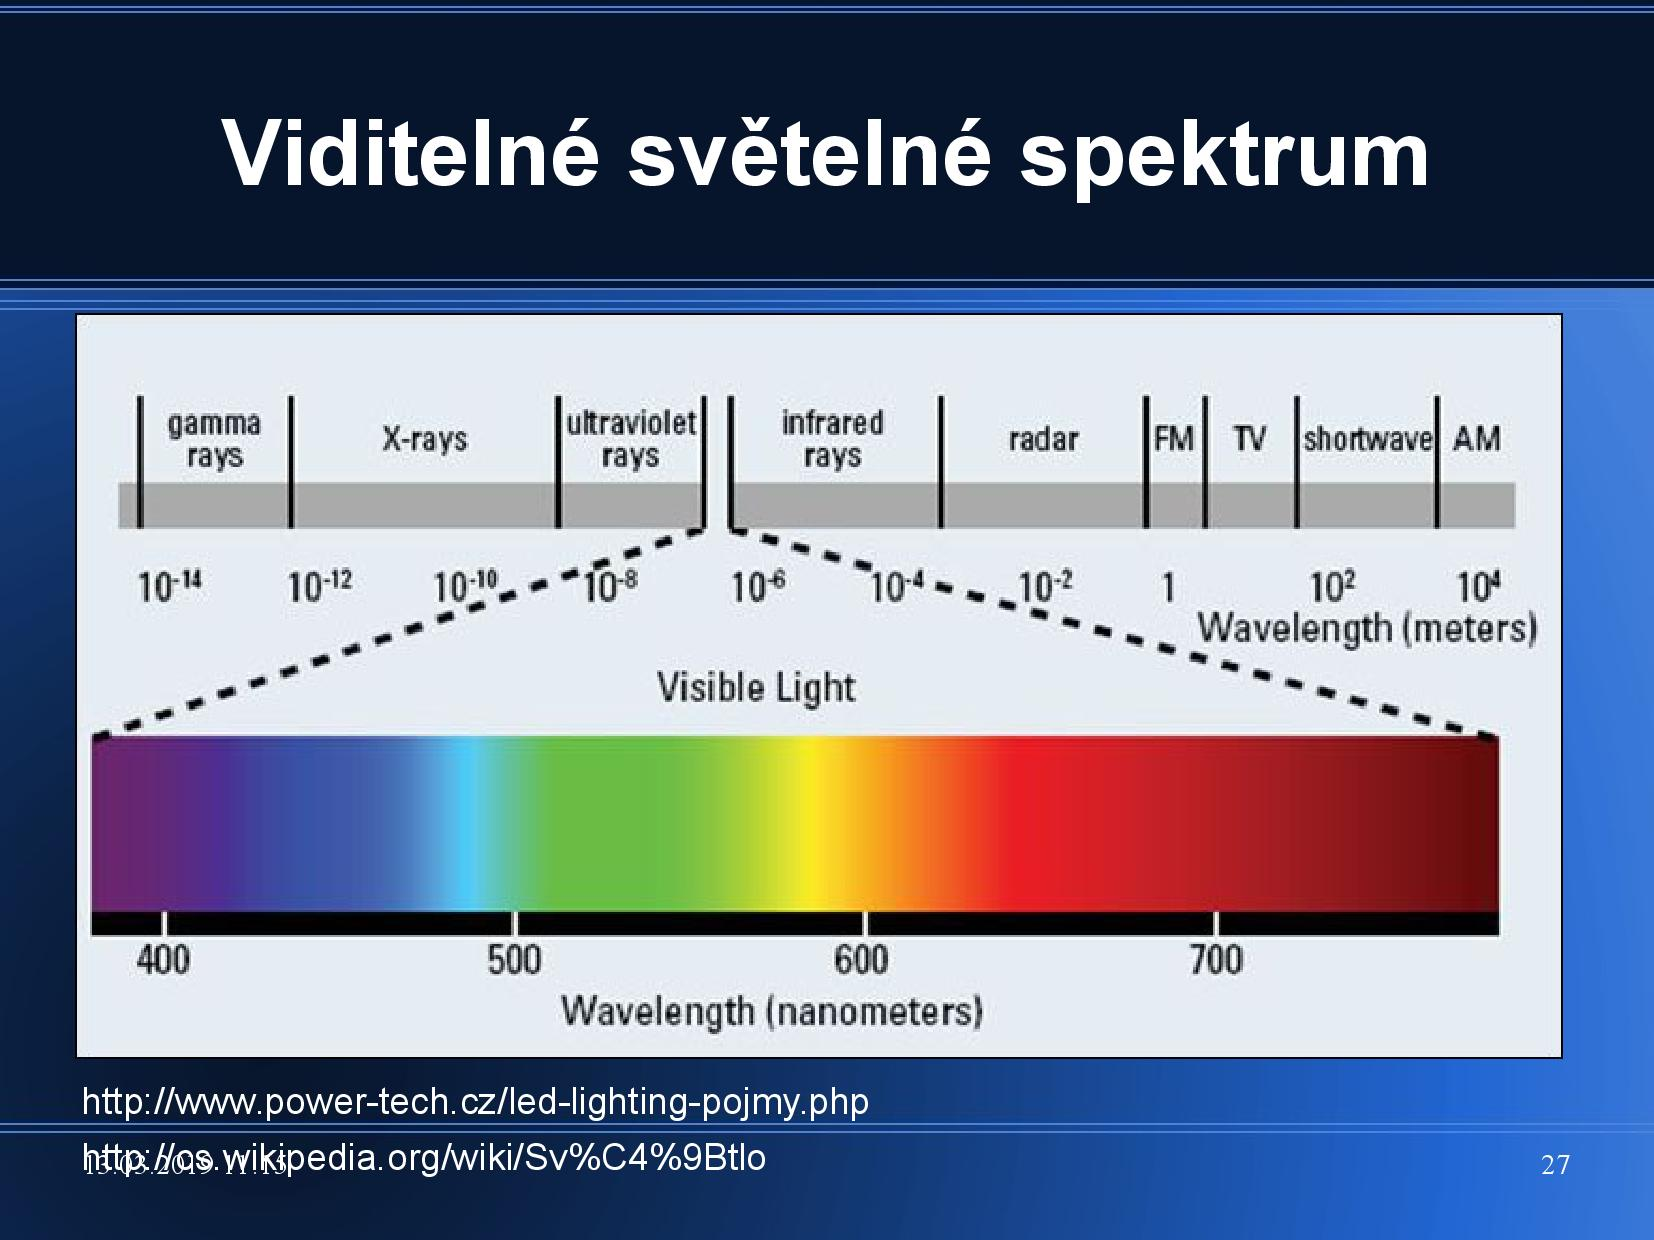
\includegraphics[width=0.85\textwidth]{slides-2/slide-27.jpg}
    \centering
    \label{slides-2-slide-27}
\end{figure}

Světlo: viditelné elektromagnetické záření. Pro spektrofotometrii (zde dále SFM) proteinů je vhodnější UV záření.

\paragraph{Lambertův-Beerův zákon}
\begin{itemize}[nosep]
    \item určuje, jakým způsobem prochází světlo vzorkem
    \item vzorek může světlo pohlcovat (na tom naříklad záleží jeho barva), nebo rozptylovat
\begin{itemize}[nosep]
    \item v obou případech pozorujeme intenzitu světla před a po projití vzorkem
\end{itemize}

\end{itemize}



Konkrétní znění zákona se dá vyjádřit vzorcem
\begin{align*}T &= \frac{I}{I_0} \\
A &= -\log T = \varepsilon \cdot l \cdot c,\end{align*}

kde \(I\) a \(I_0\) značí inzentity světla, \(T\) je \textbf{transmitance} vzorku, \textbf{A} je absorbance vzorku a \(\varepsilon\) je molární extinkční koeficient. Pokud íiž známe absorbanci naší látky, můžeme pomocí tohoto vzorce například spočítat jejich koncentraci.

\begin{figure}
    \caption{Prezentace č. 2, slide č. 32}
    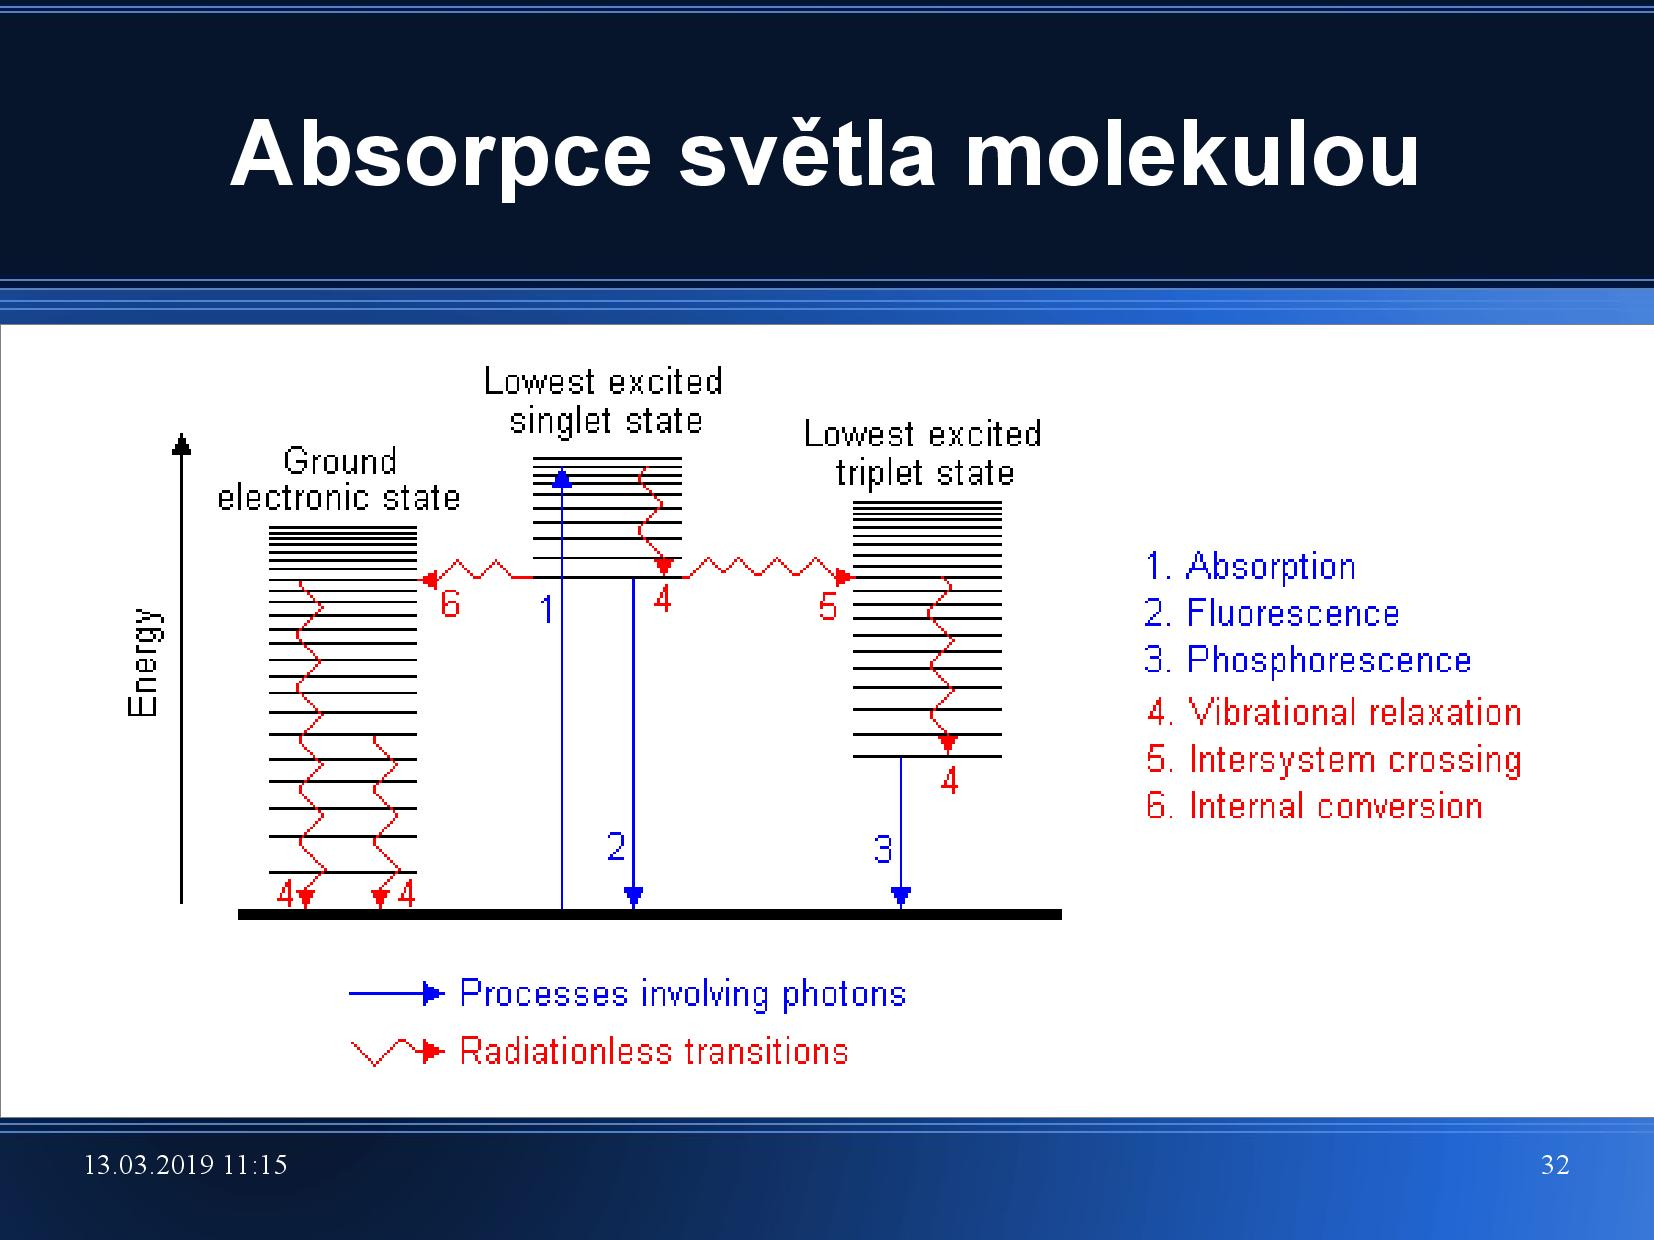
\includegraphics[width=0.85\textwidth]{slides-2/slide-32.jpg}
    \centering
    \label{slides-2-slide-32}
\end{figure}

\paragraph{Absorbce světla molekulou}
\begin{itemize}[nosep]
    \item molekula má v základním stavu
    \item po absorpci fotonu se dostane celá molekula do excitovaného stavu, protože jeden z jejích elektronů přejde do vyššího orbitalu
    \item excitovaná molekula při návratu do základního stavu vyzáří energii
    \item velikost vyzářené energie závisí na růzdílů energií orbitalů, mezi kterými elektron přecházel
\end{itemize}



\subsection{Spektrofotometrie v praxi} \label{Spektrofotometrie v praxi}


SFM je nedestruktivní metoda, což je její velká výhoda.

\begin{figure}
    \caption{Prezentace č. 2, slide č. 33}
    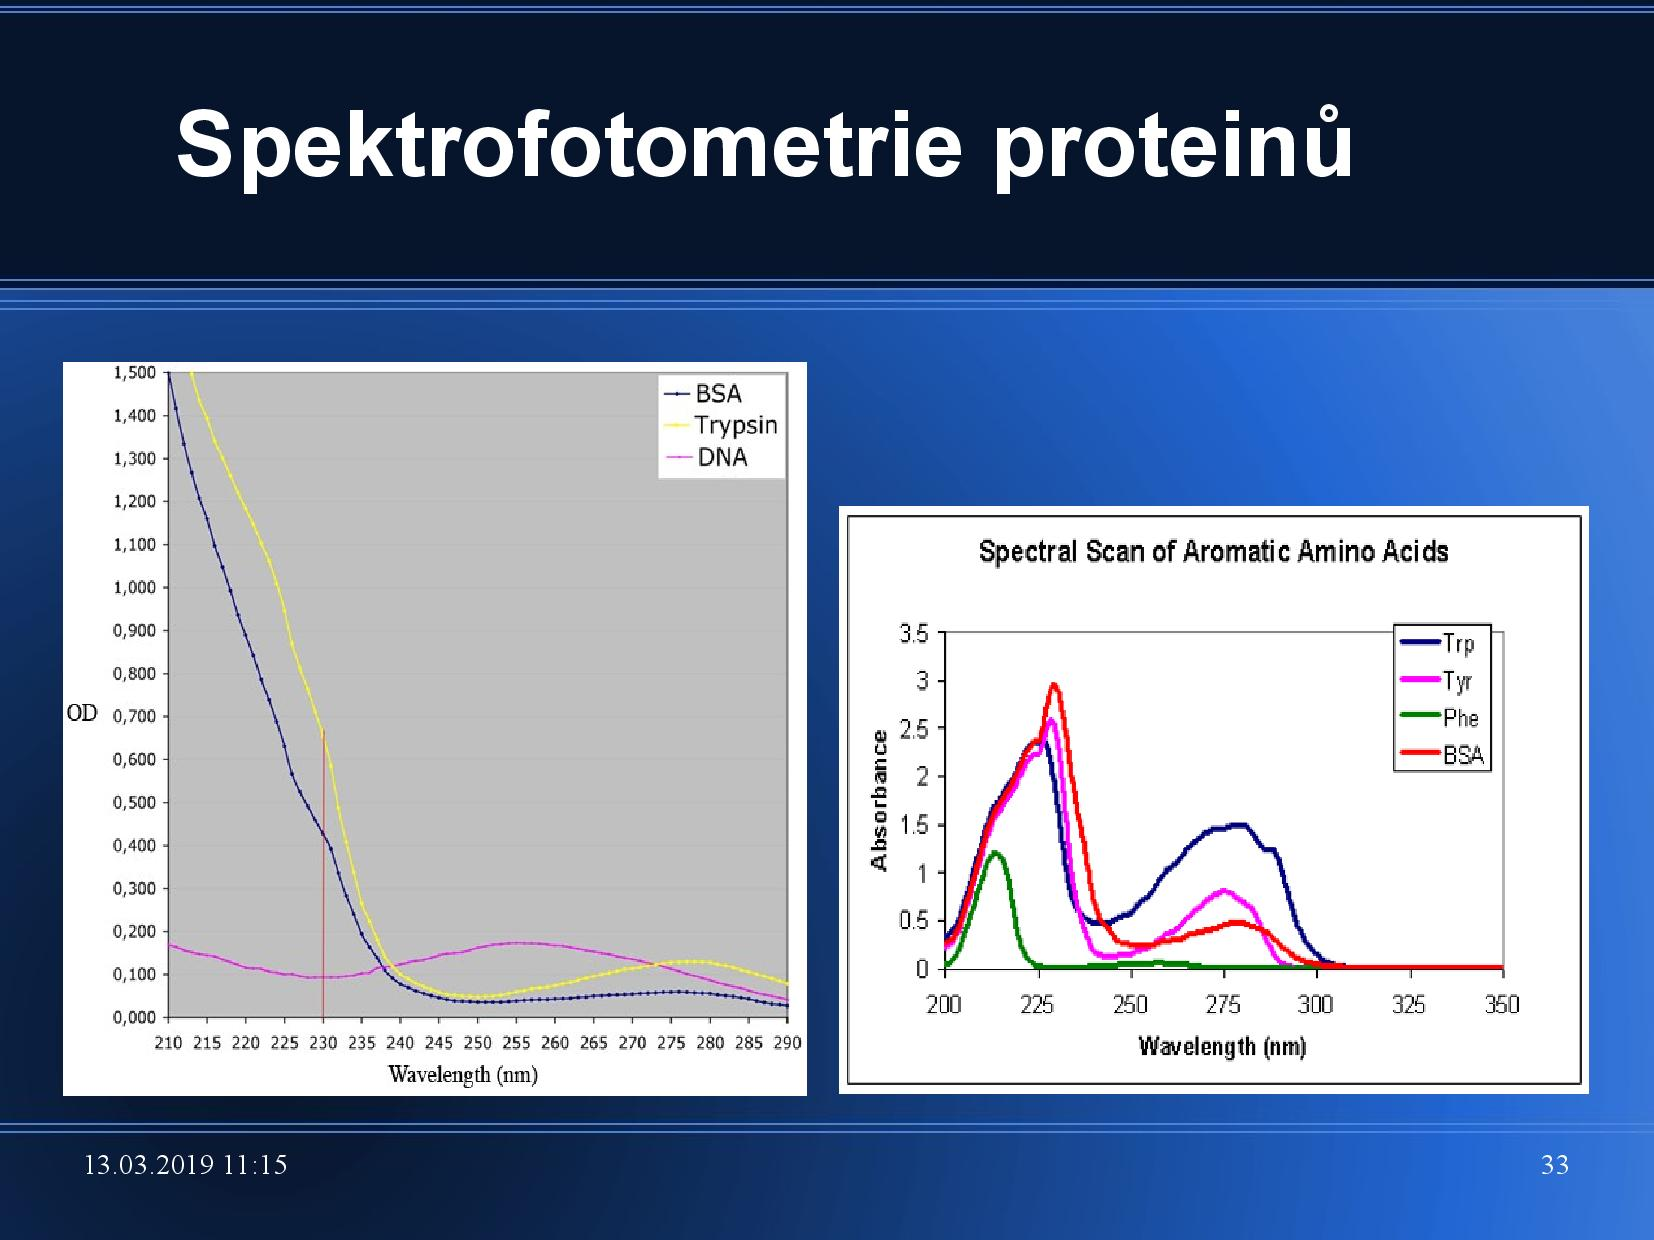
\includegraphics[width=0.85\textwidth]{slides-2/slide-33.jpg}
    \centering
    \label{slides-2-slide-33}
\end{figure}

Proteiny dobře absorbují světlo kolem 225nm (tam absorbuje peptidová vazba) a případně i kolem 260nm, když mají nějaké aromatické AK. Všechny AK absorbují různě moc, takže pokud známe složení proteinu a vidíme absorpční spektrum vzorku, umíme z něj vypočítat koncentraci. \(\varepsilon\) pro jakýkoli protein o známé sekvenci se totiž dá dopočítat.

Nukleové kyseliny zpravidla absorbují kolem 260nm. U nukleových kyslein se užívá například k posouzení stupně a průběhu denaturace, k posouzení homogenity Pro sekvence DNA a RNA se koncentrace stanovuje trochu jinak,
\[100 \cdot \frac{A_{260}}{K} = c.\]
Pro dsDNA \(K = 2\), pro ssDNA \(K = 2,5\), pro ssDNA \(K = 3\), pro oligo DNA \(K = 3,3\) -- \(K = 5\).

\section{Cirkulární dichroismus} \label{Cirkulární dichroismus}


\begin{figure}
    \caption{Prezentace č. 2, slide č. 52}
    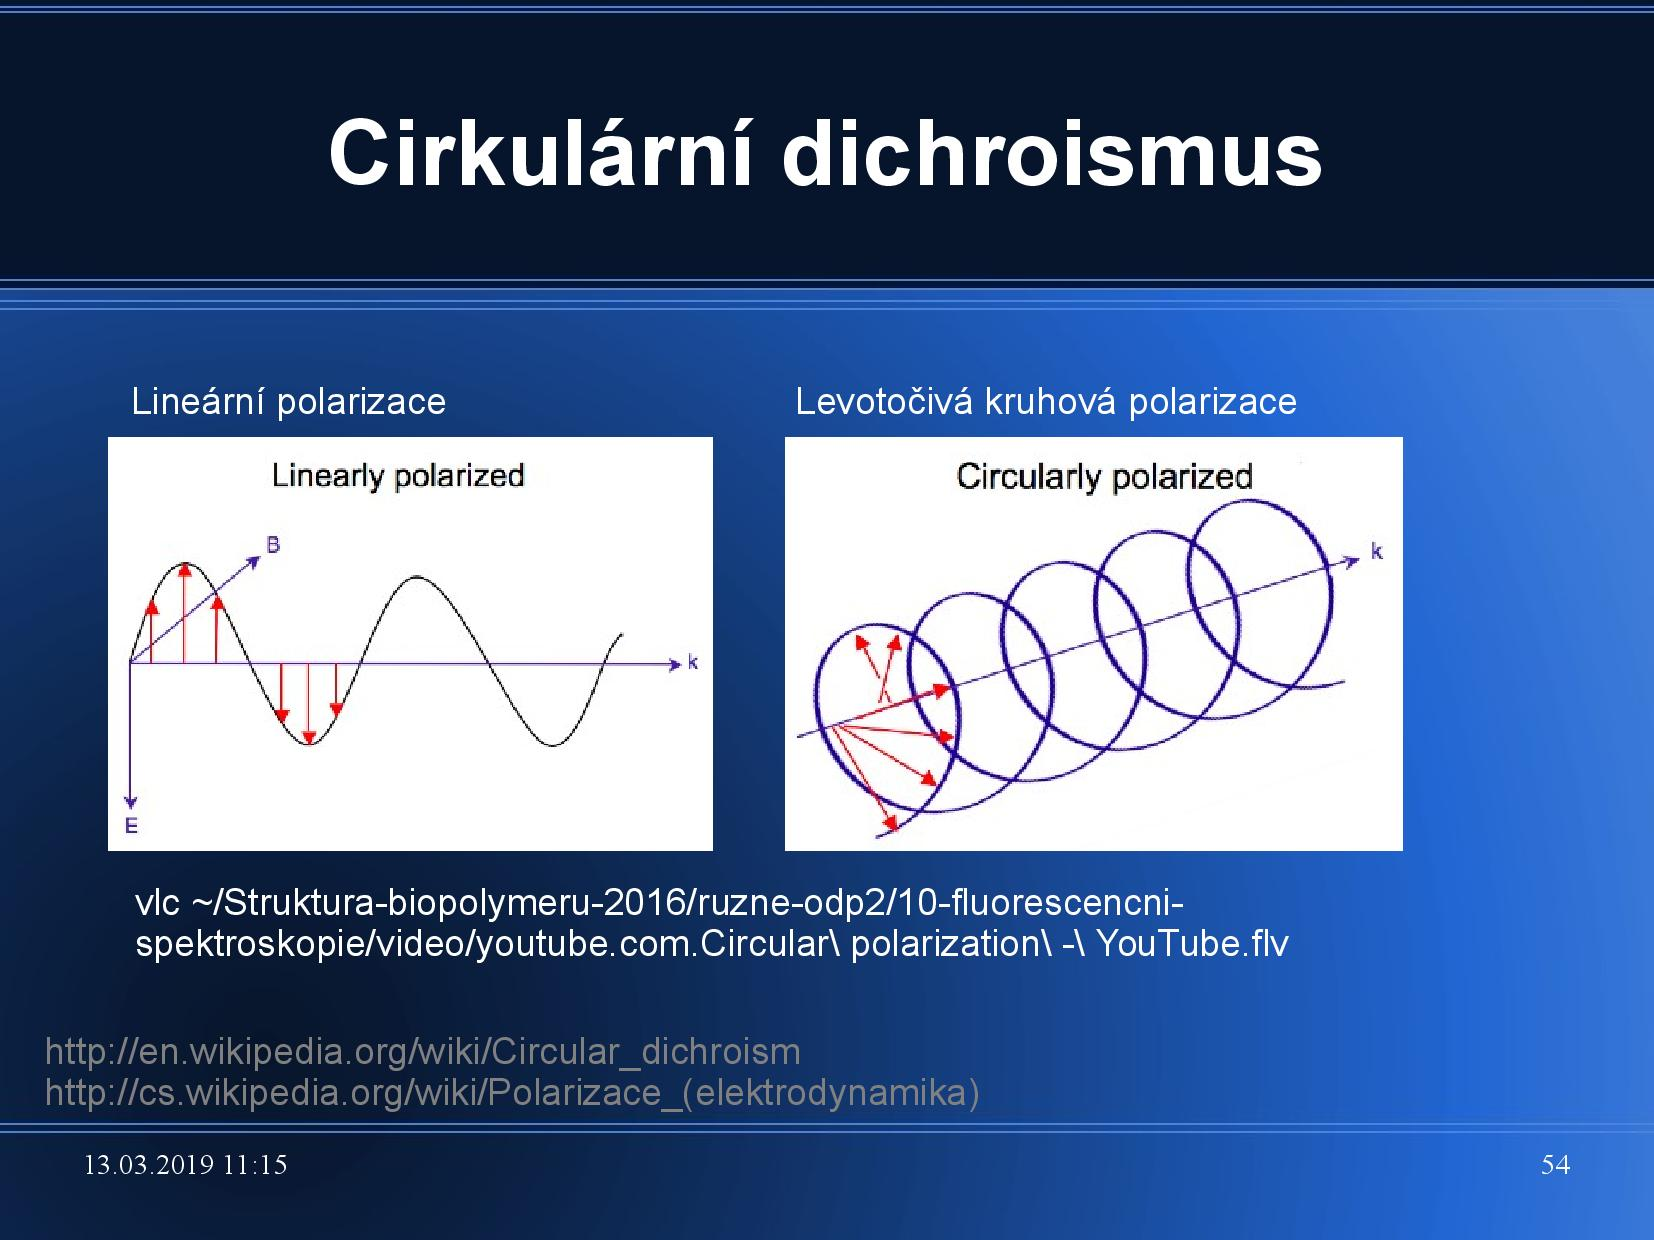
\includegraphics[width=0.85\textwidth]{slides-2/slide-52.jpg}
    \centering
    \label{slides-2-slide-52}
\end{figure}

\begin{description}
\item[lineární polarizace světla]\hfill \\
Udává rovinu kmitání elektrické vlny světla. Běžné světlo není polarizované, i když při odrazu k částečné polarizaci dochází.

Ke změně polarizace můžeme použít polarizační filtry, které propustí pouze světlo, které kmitá v jedné konkrétní rovině.


\item[cirkulární polarizace světla]\hfill \\
Pokud v polarizovaném světle zpozdíme kmitání magnetické složky, například o čtvrt vlny, výsledný světelný vektor, který se součtem vektoru elektrického pole a vektoru magnetického pole, se bude postupně při kmitání otáček.

Rozlišujeme pravotočivou a levotočivou polarizaci.

\end{description}


Absorbce cirkulárně polarizovaného světla záleží na chiralitě molekul a na levotočivosti a pravotočivosti světla. \textbf{Cirkulární dichroismus} je rozdíl mezi absorbancí levotočivě a pravotočivě polarizovanho světla.

Cirkulární dichroismus jednotlivých SS se liší, viz obrázek. Podobně se liší CD pro protein s nějakým foldem a denaturovaný protein. Pokud změříme CD proteinu, můžeme z výsledné spektrální křivky zjistit procentuální podíl jednotlivých SS.

\begin{figure}
    \caption{Hodnota cirkulárního dichroismu pro různé sekundární struktury}
    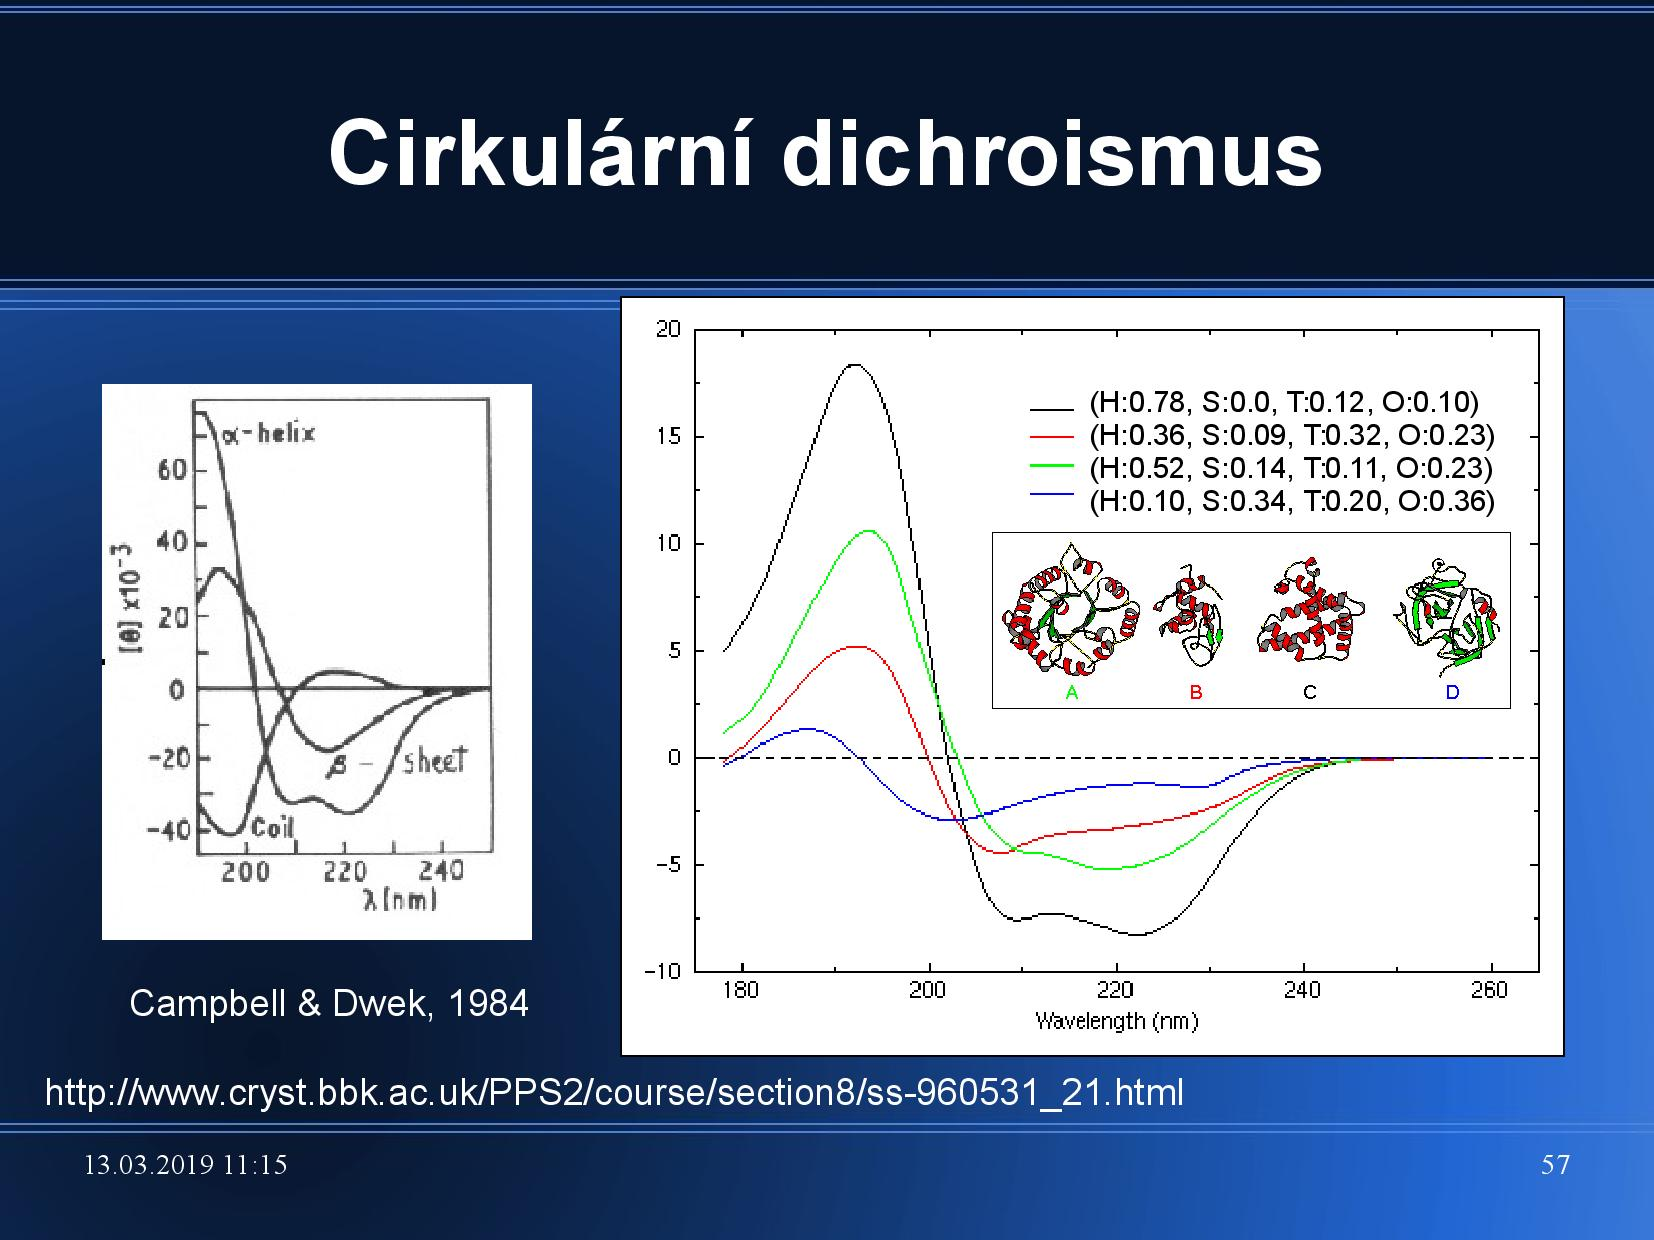
\includegraphics[width=0.85\textwidth]{slides-2/slide-55.jpg}
    \centering
    \label{}
\end{figure}


\section{Gelová elektroforéza} \label{Gelová elektroforéza}


Pomocí ELFO můžeme zjistit velikost proteinu, odhalit počet proteinů nebo odhalit kontaminaci vzorku. Nejběžnější forma je \textbf{SDS-PAGE}, SDS polyakrylamidová gelová elektroforéza.

\begin{figure}
    \caption{Prezentace č. 2, slide č. 37}
    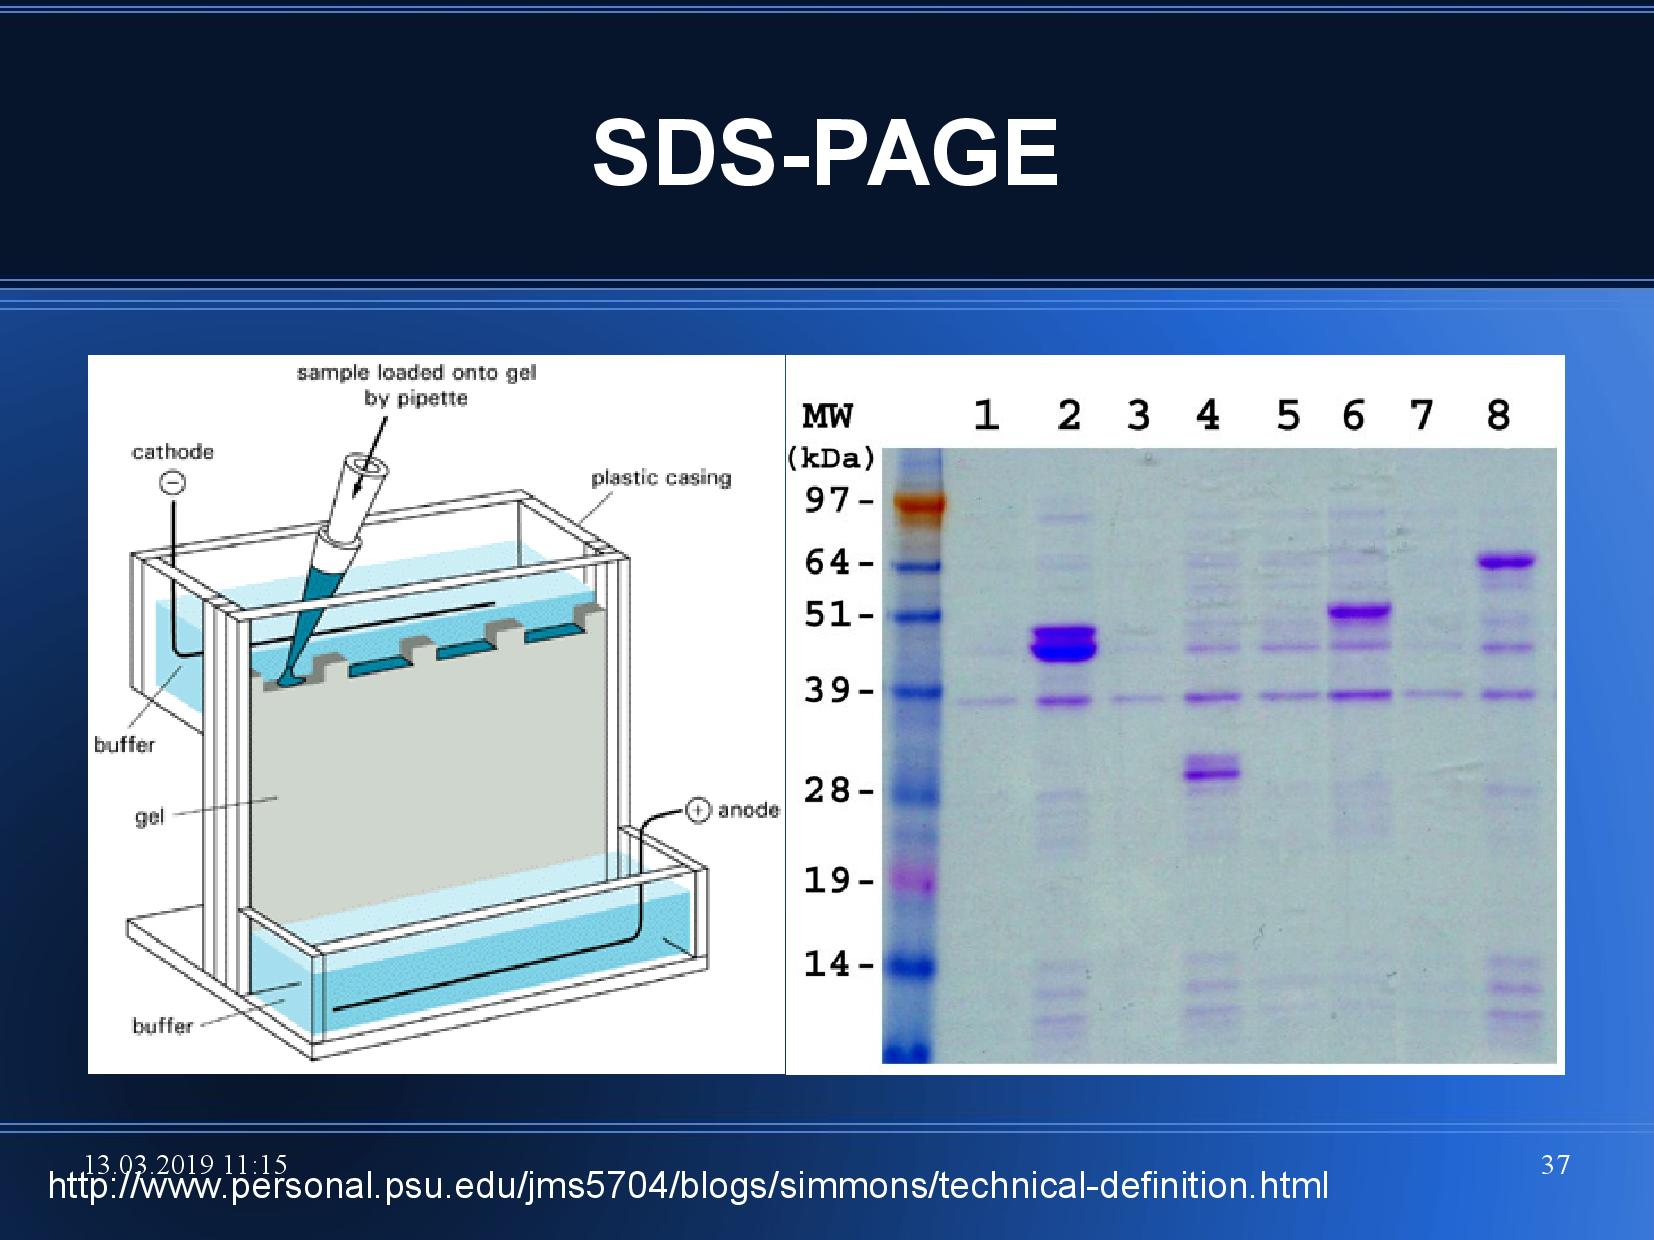
\includegraphics[width=0.85\textwidth]{slides-2/slide-37.jpg}
    \centering
    \label{slides-2-slide-37}
\end{figure}
\begin{figure}
    \caption{Prezentace č. 2, slide č. 45}
    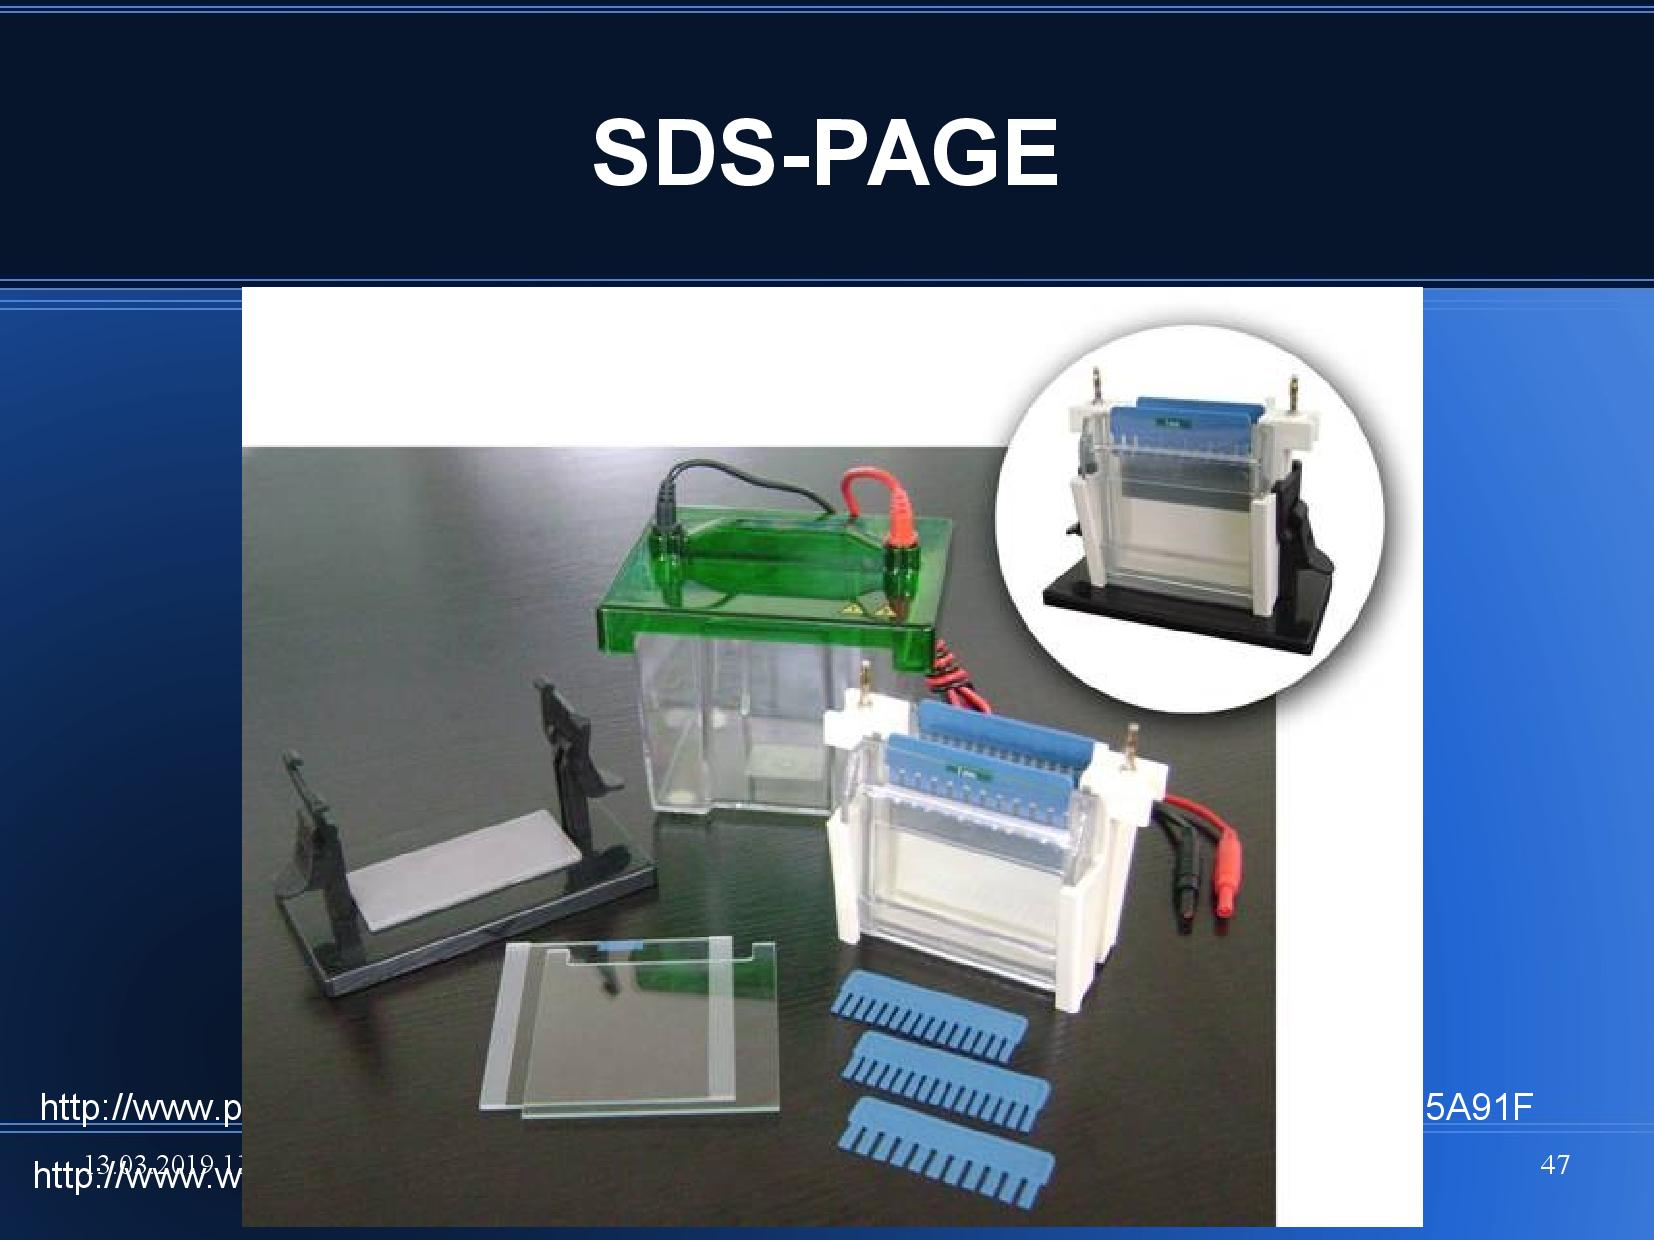
\includegraphics[width=0.85\textwidth]{slides-2/slide-45.jpg}
    \centering
    \label{slides-2-slide-45}
\end{figure}

\paragraph{Základní princip ELFO}
\begin{enumerate}[nosep]
    \item do gelu dáme do několika řad (line) vzorky (zpravidla nahoru)
    \item na gelu vytvoříme elektrické napětí
    \item všechny vzorky putují na druhou stranu gelu (zpravidla dolů), jejich ryhlost se (ideálně) liší pouze podle jejich velikosti
    \item po vypnuté elektrického proudu máme nedál od startu nejlehčí vzorky, nejblíže jsou vzorky nejtěžší
\end{enumerate}



Musíme zařídit, aby byl gel tak akorát hustý, a aby všechny vzorky opravdu putovaly na stejnou stranu gelu (ke stejné elektrodě). Zároveň by bylo dobré nakonec vzorky nějak obarvit, ať je vůbec vidíme.

Protože nechceme proteiny dělit podle jejich tvaru, ale jen podle velikosti, povaříme je před ELFO v denaturačních činidlech.

\subsection{Gel} \label{Gel}


Polyakrylamidový gel je sice velice náročný na přípravu, má ale výborné rozlišovací schopnosti: například při dělení DNA lze rozpoznat DNA dlouhou 500bp od 501bp.

\begin{itemize}[nosep]
    \item polykarylamidový gel, nejčastěji 3\%--15\%
    \item \(\ce{akrylamid + bisakrylamid}\)
\begin{itemize}[nosep]
    \item vzniknou zesíťovaná vlákna
    \item aby proběhlaradikálová polymerace, potřebujeme také iniciátor (persíran amonný nebo UV-ozářený riboflavin) a stabilizátor volných radikálů (TEMED)
    \item musí probíhat v anaerobních podmínkách
\end{itemize}

    \item jeho viskozita zajišťuje, že velikým molekulám je při pohybu kladen větší odpor než malým
\begin{itemize}[nosep]
    \item tato konkrétní vlasnost záleží na jeho koncentraci, pro různé vzorky se používají různě koncetrované gely
    \item pro srovnání velmi rozdílných vzorků se používají \textbf{gradientové gely}, jejichž hustota se seshora dolů zvyšuje
\end{itemize}

\end{itemize}



Na tento gel se nanáší ještě \emph{zaostřovací gel}, přechod mezi ním a PAG pak tvoří jakousi "startovací linii", na kteoru se seřadí a vyrovnají porovnávané vzorky.

\subsection{SDS} \label{SDS}


\begin{figure}
    \caption{Prezentace č. 2, slide č. 46}
    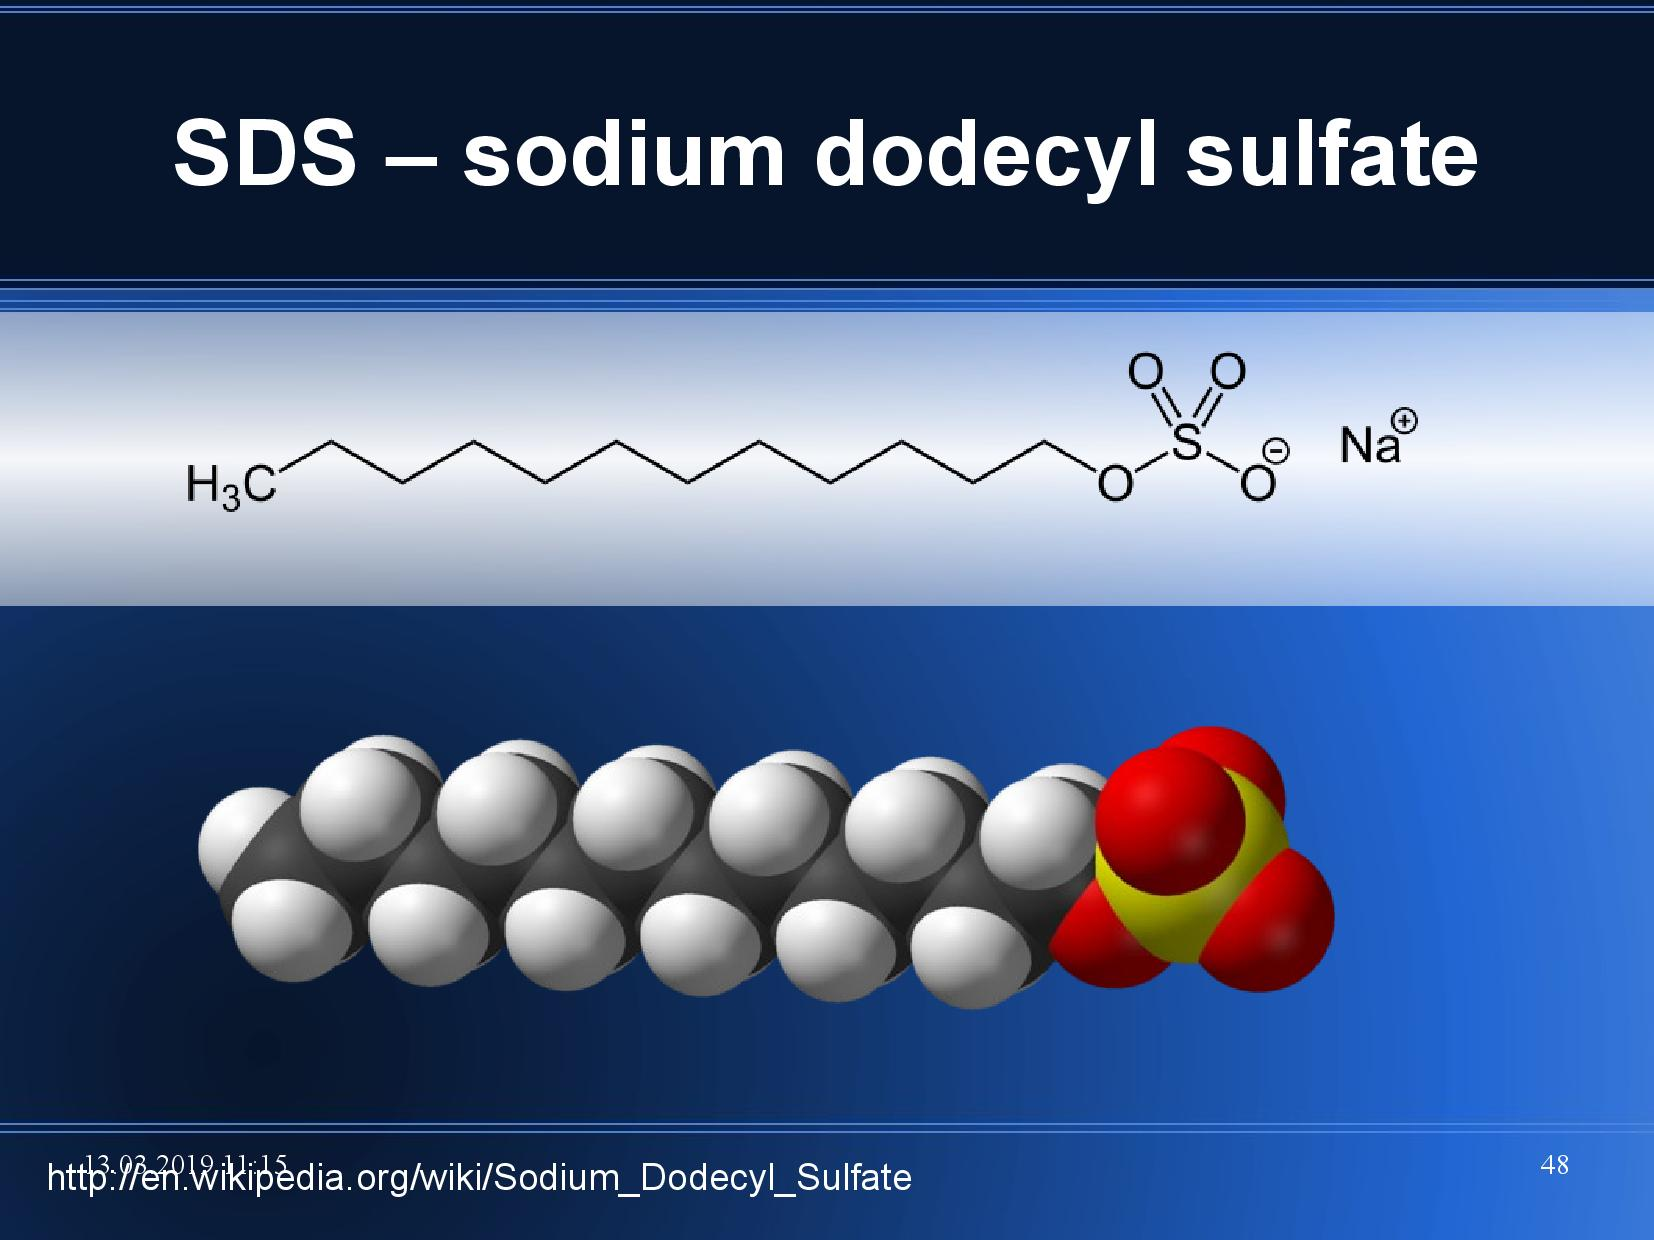
\includegraphics[width=0.85\textwidth]{slides-2/slide-46.jpg}
    \centering
    \label{slides-2-slide-46}
\end{figure}

SDS (sodium dodecyl sulfát) se váže na proteiny. Velké proteiny vážou více SDS než malé proteiny. SDS má dvojí význam:
\begin{enumerate}[nosep]
    \item zabraňuje tomu, aby se proteiny samovolně opět nafoldovaly
    \item má záporný náboj, který "přebije" náboj proteinů a všechny proteiny tím pádem budou putovat ke kladné elektrodě
\begin{itemize}[nosep]
    \item větší proteiny sice budou taženy větší silou, ale zase budou více brzděny gelem
\end{itemize}

\end{enumerate}



\subsection{Barvení} \label{Barvení}


Proteiny chceme samozřejmě nějak vizualizovat, aby nám ELF ovůbec k něčemu byla.

\begin{figure}
    \caption{Prezentace č. 2, slide č. 48}
    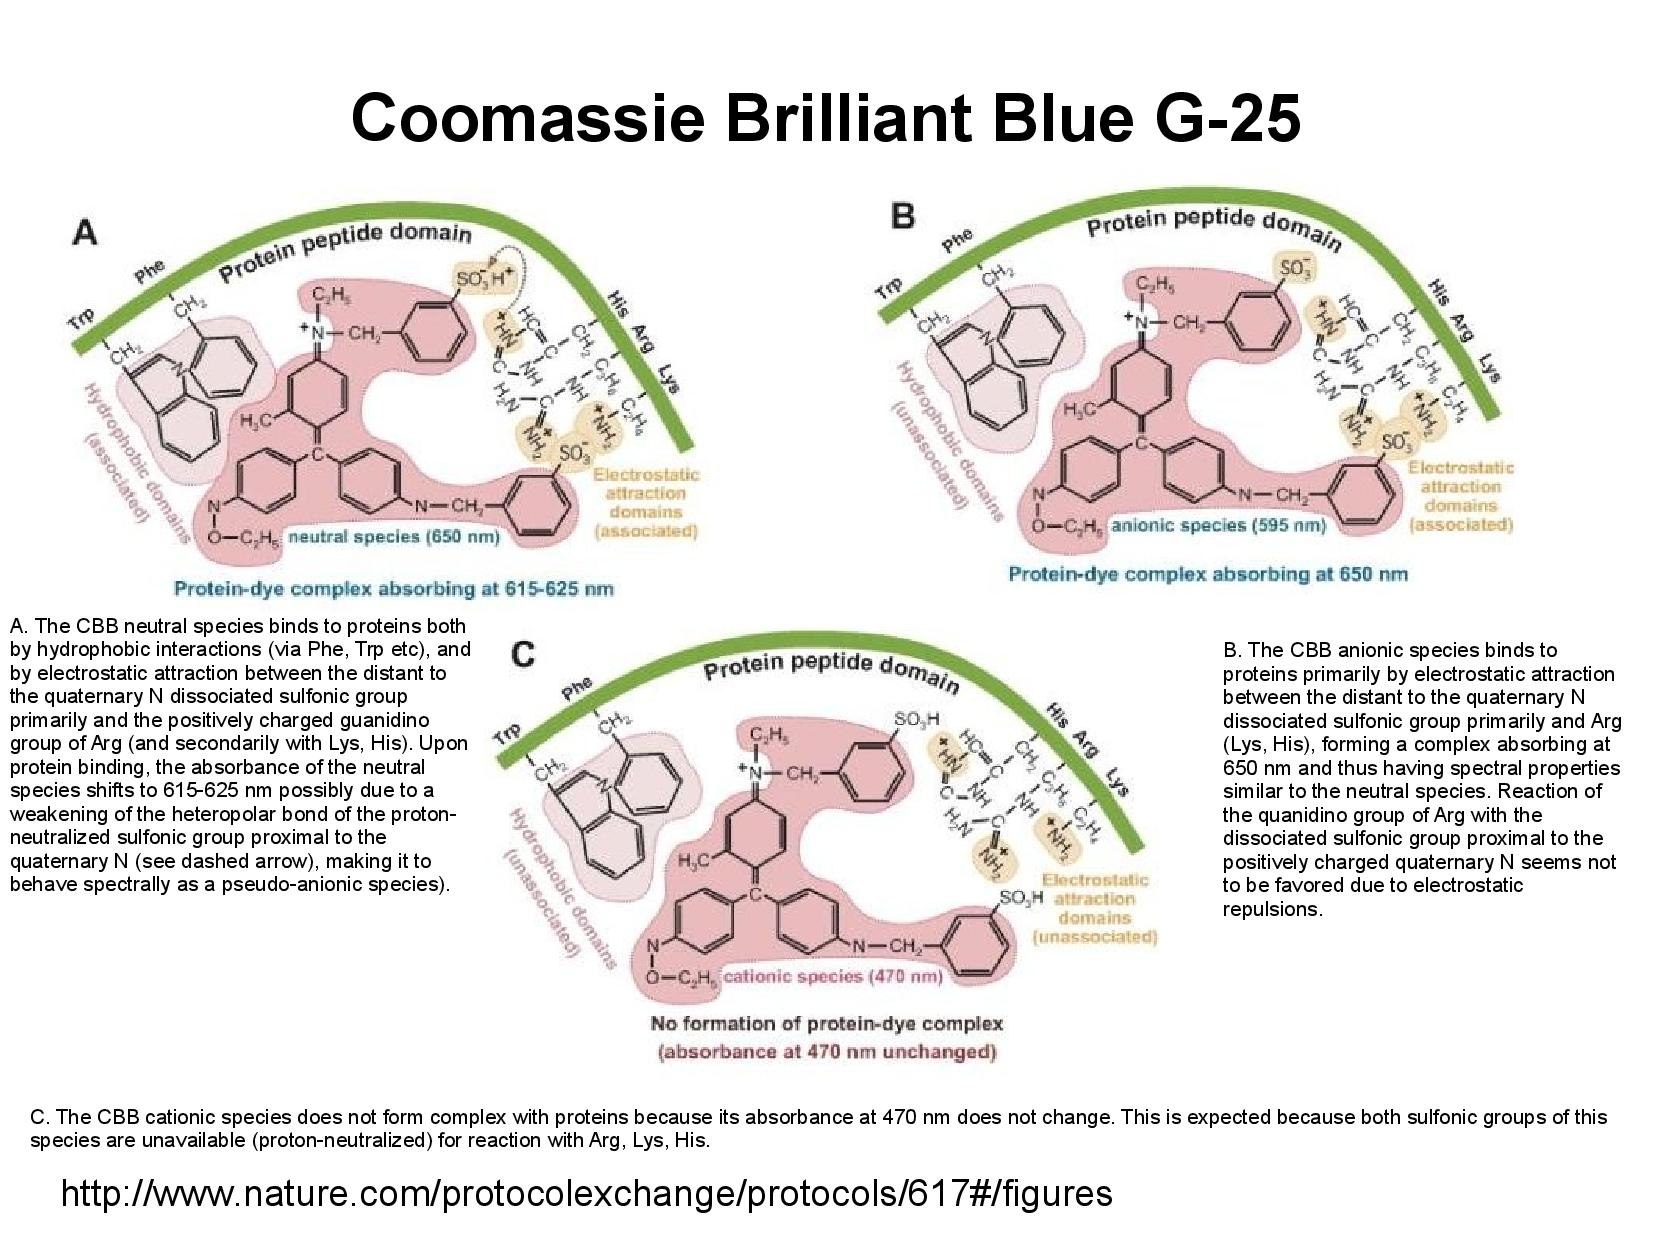
\includegraphics[width=0.85\textwidth]{slides-2/slide-48.jpg}
    \centering
    \label{slides-2-slide-48}
\end{figure}
\begin{figure}
    \caption{Prezentace č. 2, slide č. 49}
    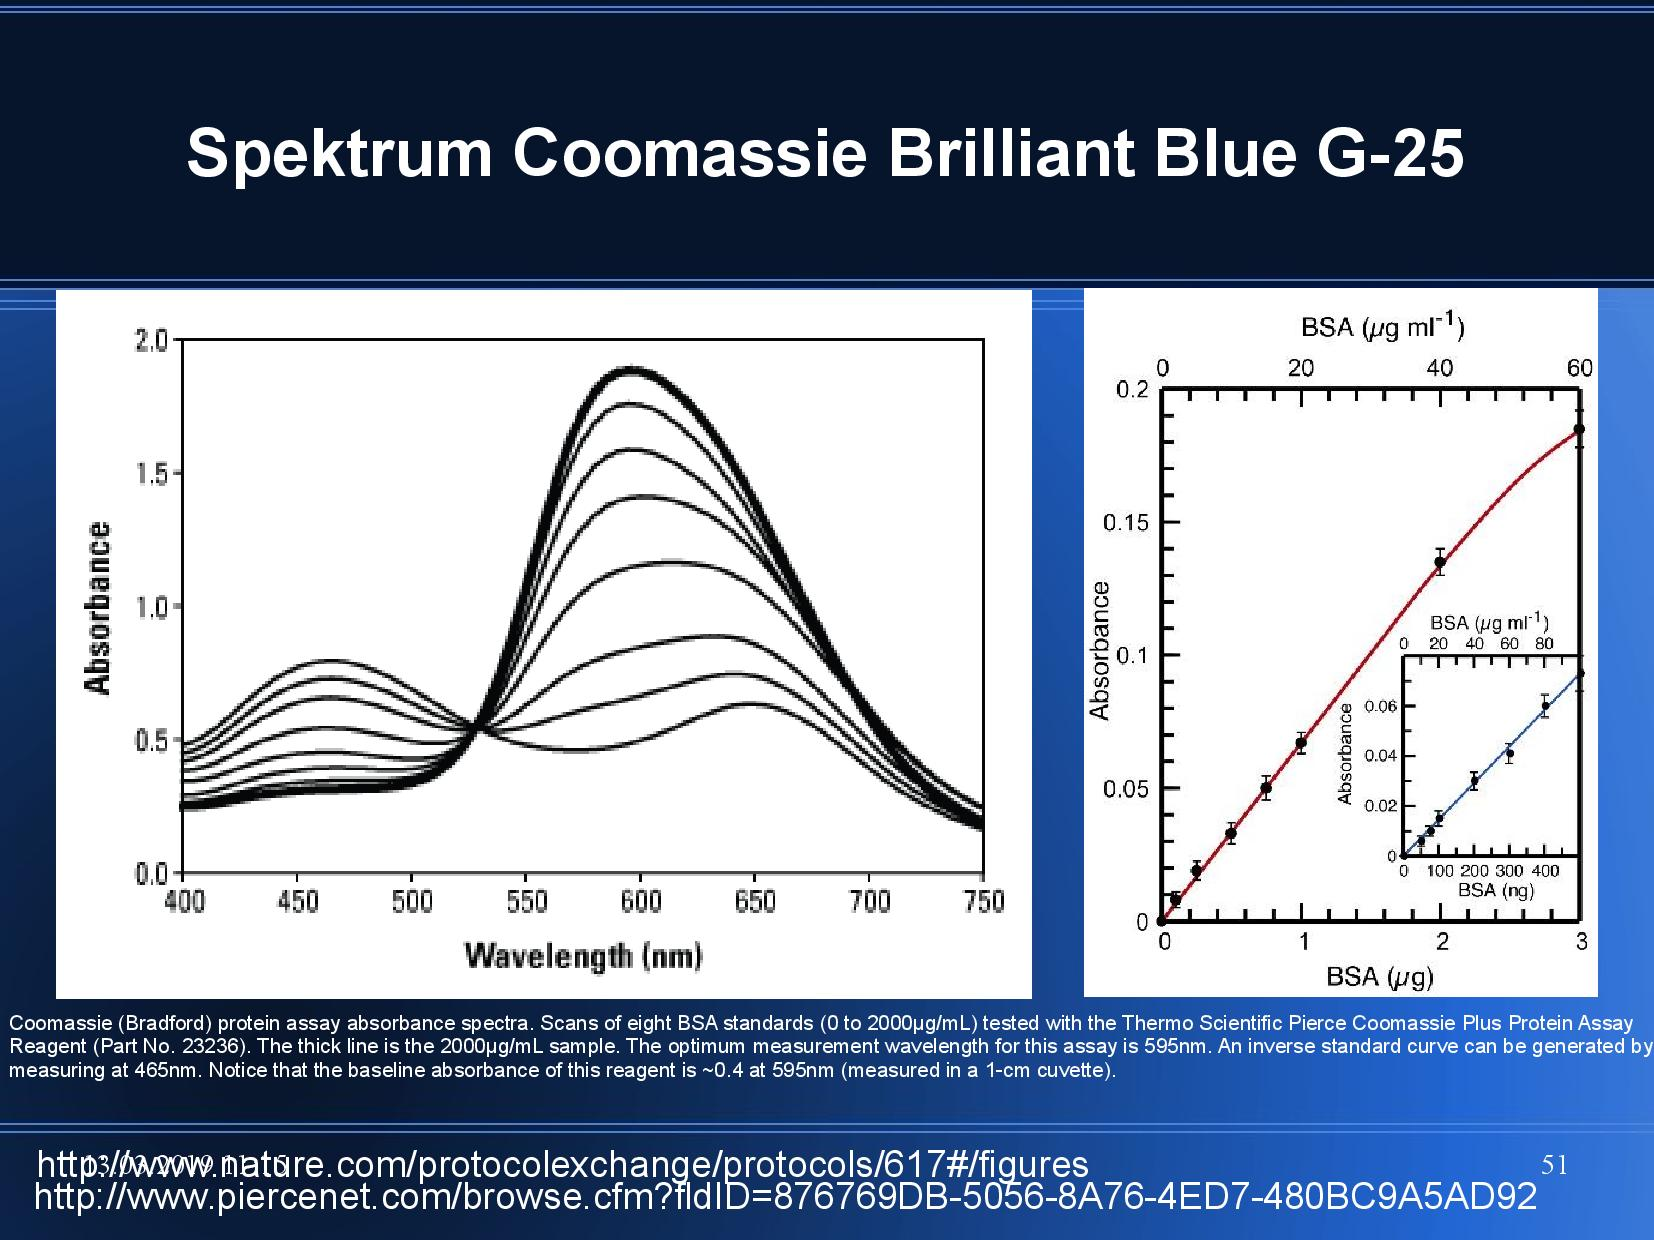
\includegraphics[width=0.85\textwidth]{slides-2/slide-49.jpg}
    \centering
    \label{slides-2-slide-49}
\end{figure}

\paragraph{Coomassie Brilliant Blue}
\begin{itemize}[nosep]
    \item nejběžnější barvivo
    \item běžně má hnědooranžovu barvu, ale když se naváže na protein, změní barvu na modrou
\begin{itemize}[nosep]
    \item váže se několikerým způsobem, vždy ale mění barvu
    \item množství proteinu se dá posoudit podle toho, jak moc modrý je výsledný obarvný roztok
\end{itemize}

\end{itemize}



Intenzita proužku vypovídá o tom, jak moc koncetrované jsou v daném místě proteiny. Zároveň ale platí, že malé proteiny se obarvují hůře, takže nebudou tak výrazné.

\section{Fluorescence} \label{Fluorescence}


\begin{description}
\item[fluorescence]\hfill \\
Světlo emitované atomem po absorbci elektromagnetického záření. Energie fluorescence pochází z přechodu částice z prvního excitovaného stavu \(S_1\) do základního elektronového stavu \(S_0\). Délka fluorescence je v řádu nanosekund.

\end{description}


\paragraph{Výhody}
\begin{itemize}[nosep]
    \item citlivost vůči okolí molekuly (teplota, viskozita, polarita, pH atd.)
    \item vhodná doba trvání
    \item citlivost (nM koncentrace analyzováneho vzorku)
    \item možnost provádět pokusy s jednotlivými molekulami (protože snímáme jednotlivé fotony)
\end{itemize}



Schéma fluorometru: na fluoreskující vzorek svítíme monochromatickým paprskem, měříme emisní spektrum.

\begin{figure}
    \caption{Schéma fluorometru}
    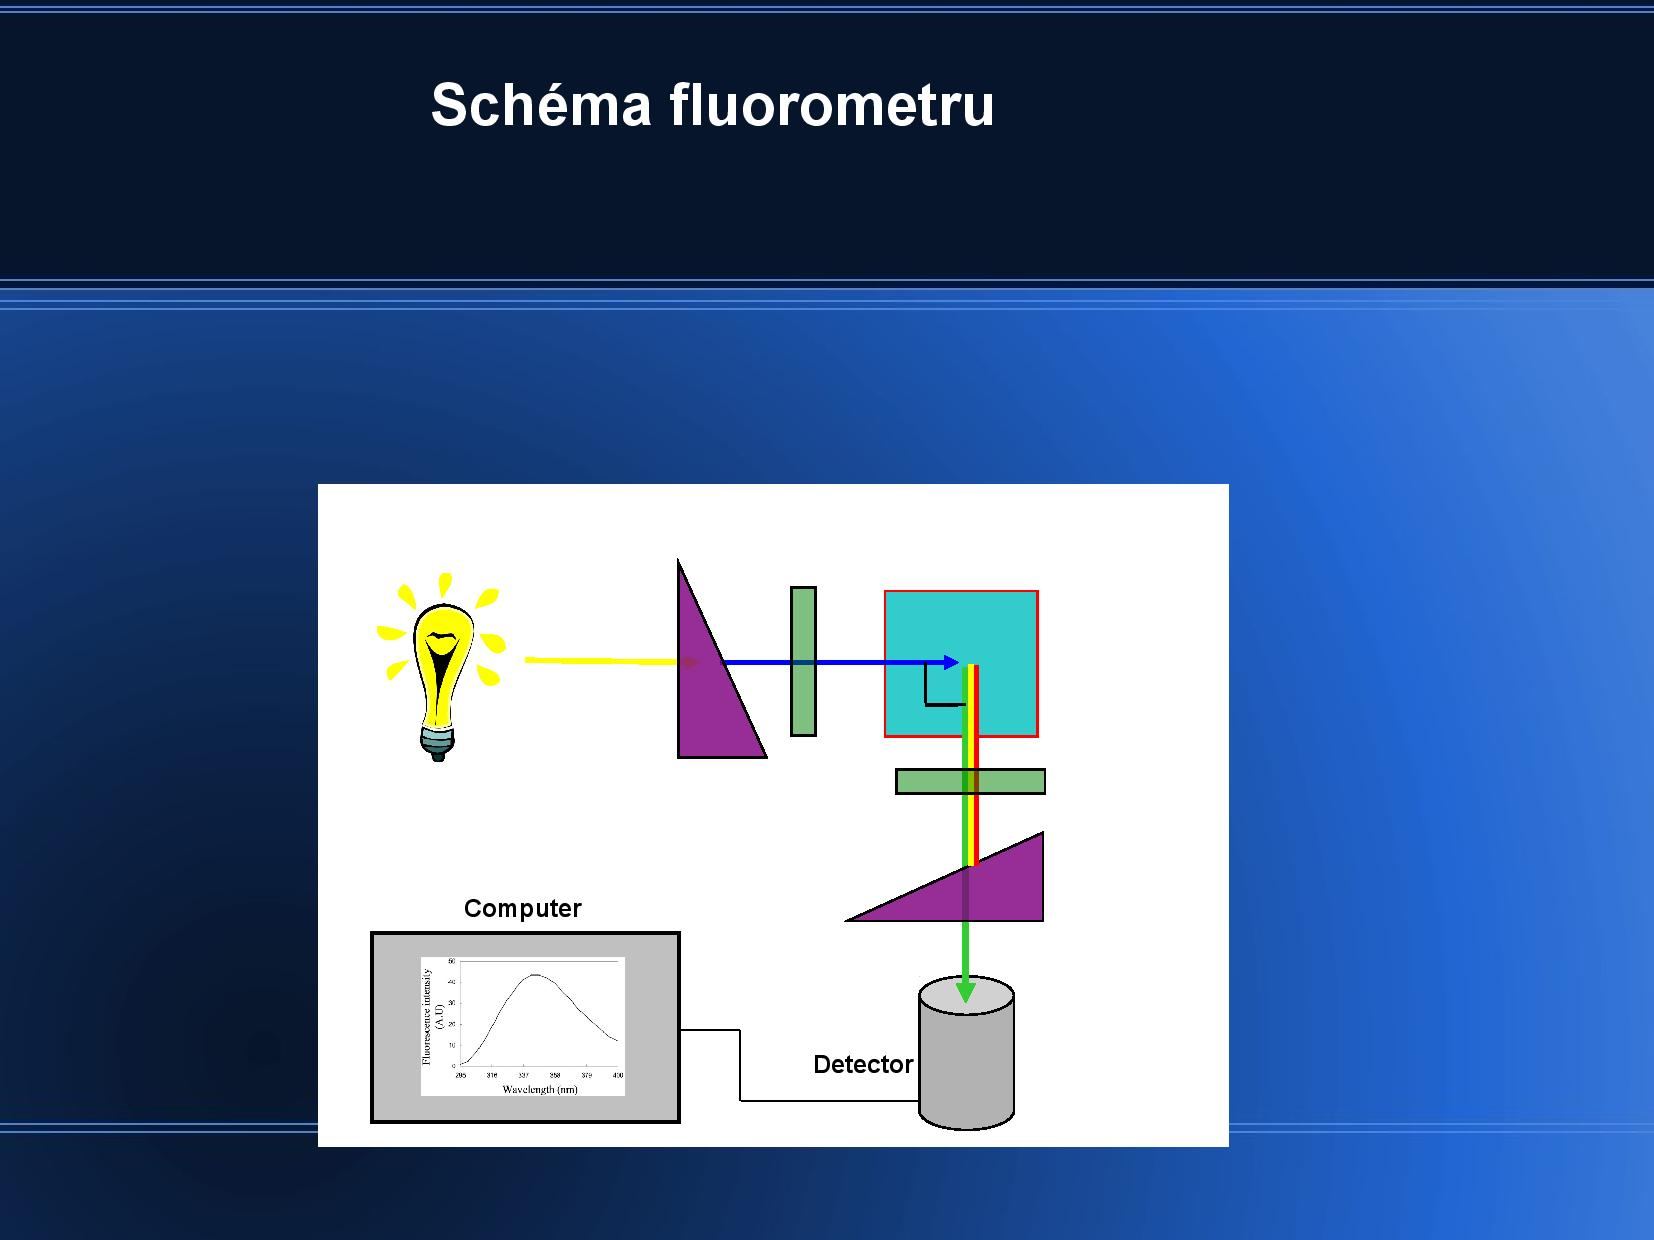
\includegraphics[width=0.85\textwidth]{slides-2/slide-61.jpg}
    \centering
    \label{}
\end{figure}


\begin{figure}
    \caption{Prezentace č. 2, slide č. 62}
    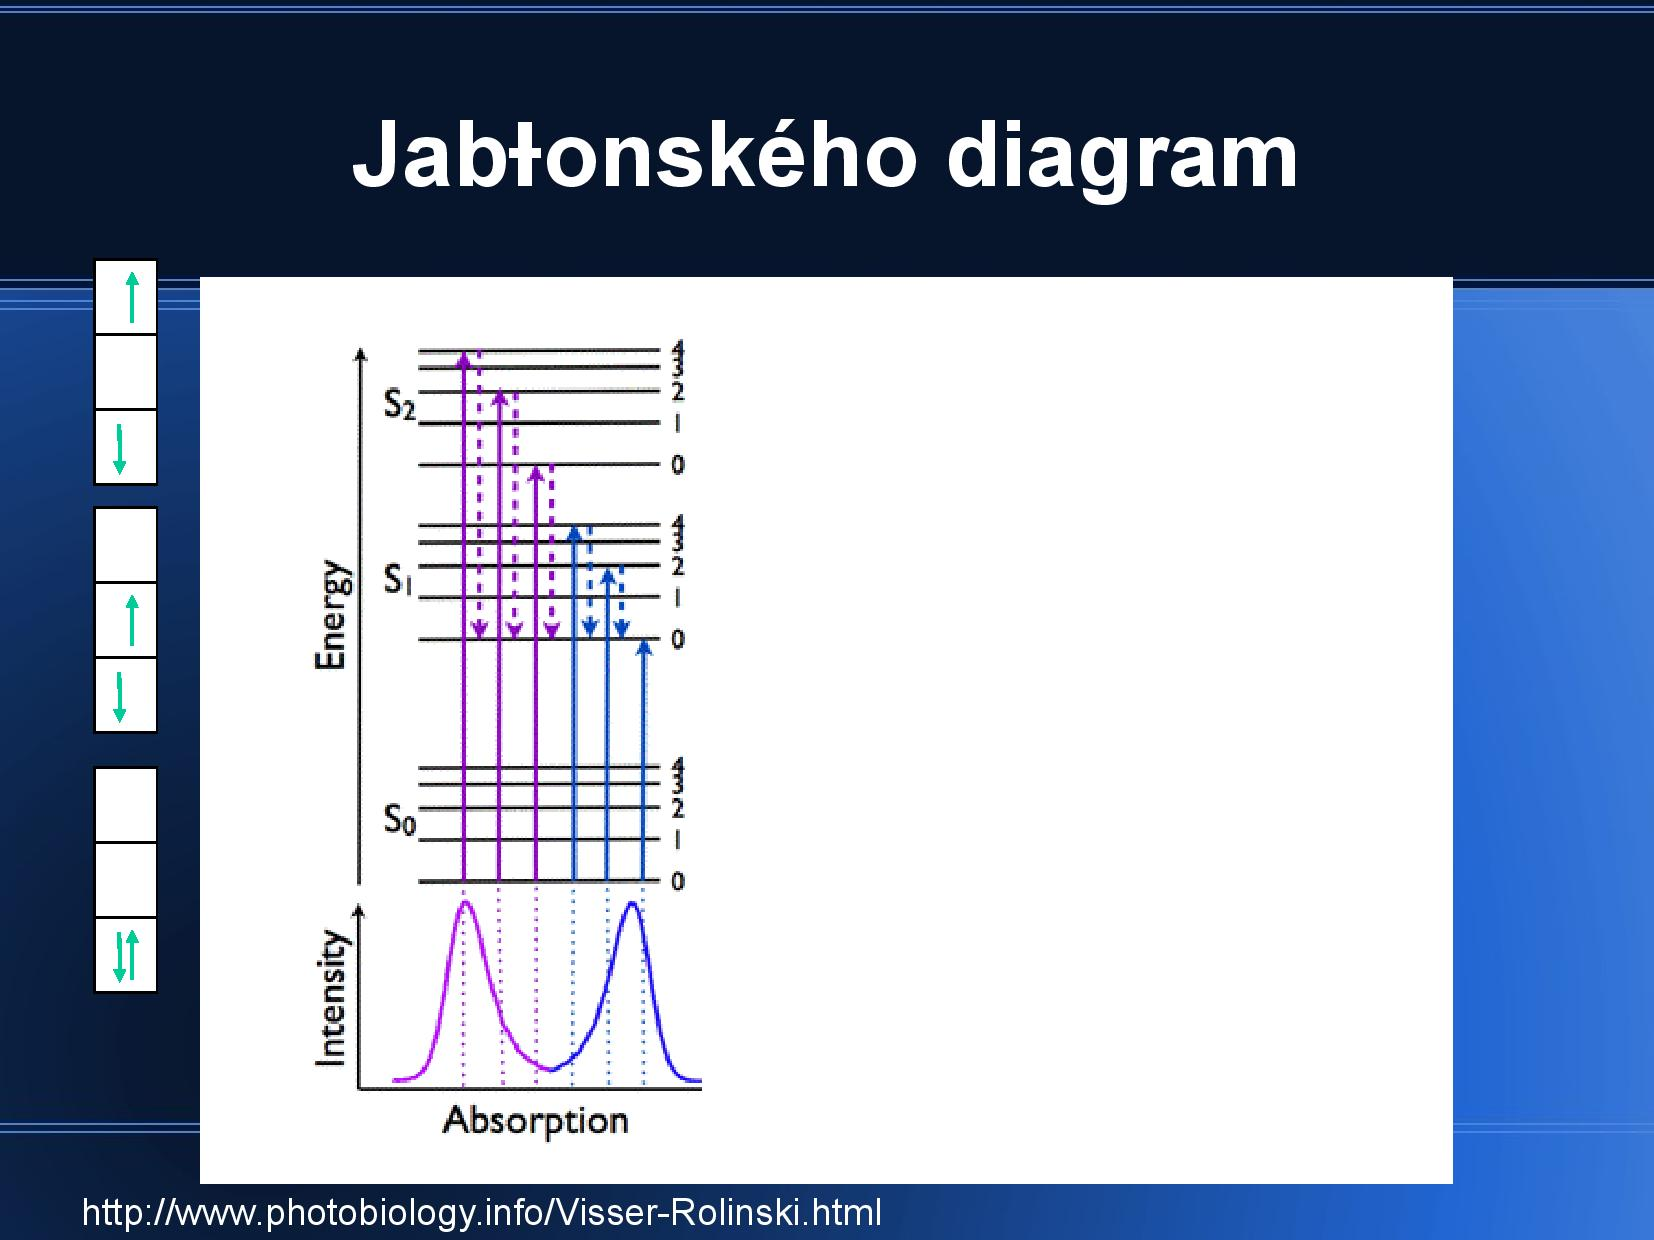
\includegraphics[width=0.85\textwidth]{slides-2/slide-62.jpg}
    \centering
    \label{slides-2-slide-62}
\end{figure}

\paragraph{Jabłonského diagram}
\begin{itemize}[nosep]
    \item rozebírá vibrační hladiny zákadního stavu \(S_0\) a jejich schopnost absorbovat světlo, viz slide
    \item vlnová délka světla musí odpovídat rozdílům energií mezi energetickými slupkami
    \item absorpční a emisní spektra jsou si podobná
\end{itemize}



\begin{figure}
    \caption{Prezentace č. 2, slide č. 64}
    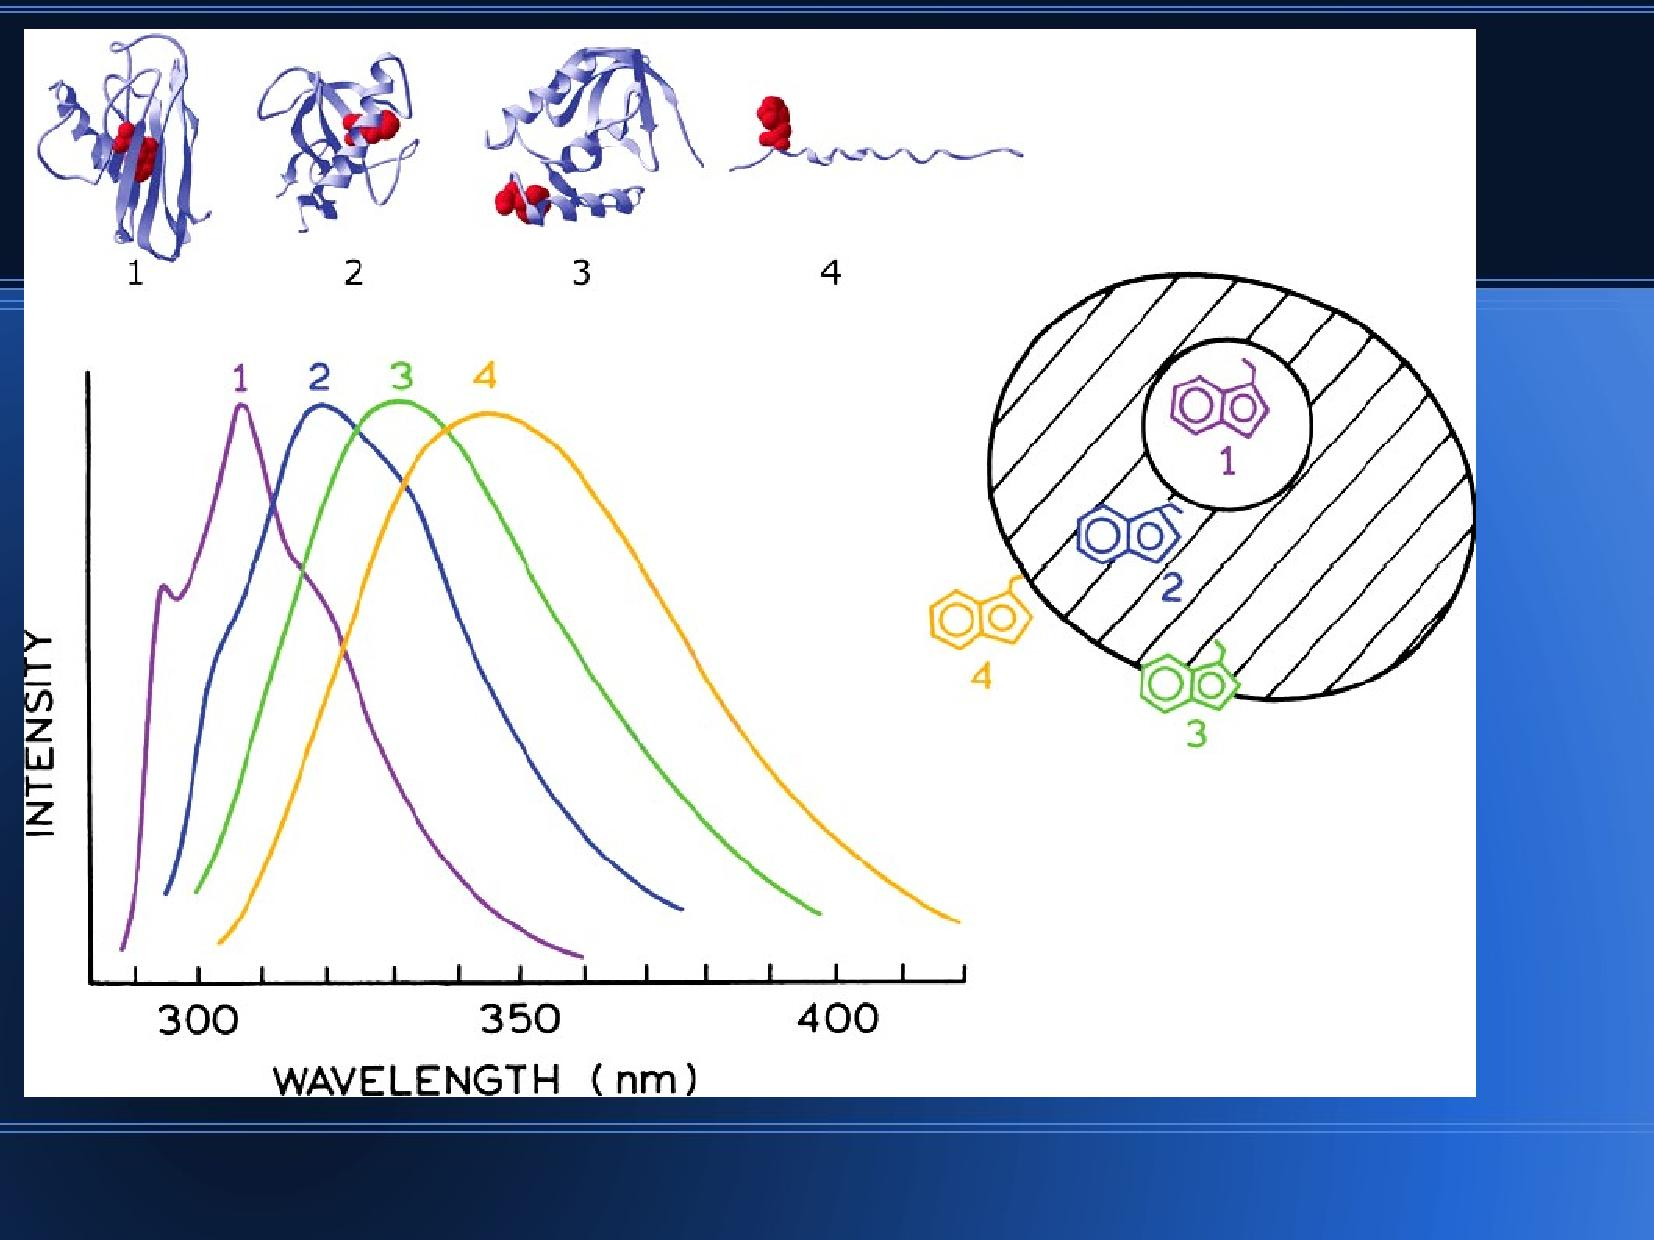
\includegraphics[width=0.85\textwidth]{slides-2/slide-64.jpg}
    \centering
    \label{slides-2-slide-64}
\end{figure}

Z emisních spekter Trp můžeme poznat, v jakém prostředí (solventu) se nachází a jestli je uvnitř či na povrchu proteinu. Posun k červené oblasti (ale stále v rámci UV) ukazuje na přítomnost \(\ce{H20}\).

\chapter{Nové zápisky v metodách} \label{Nové zápisky v metodách}


\begin{itemize}[nosep]
    \item chceme znát i více věcí než je nstrukturu
    \item koncentrace, mol.hmotnost, sekvence (introny x exony -- sekvenace proteinů), SS, rozměry a tvar molekuly
    \item až po těchto věceh zjistíme 3D strukturu
    \item a až poté řešíme interakce mezi proteiny, dynamiku a mechanismus sbalování
\end{itemize}



\mybox{TODO}{Co je Assay?}


== KONCENTRACE proteinů
- spektrofotometrie: 280 / 220 nm
- kolorimetrie
    - biuretová reakce a Cu(II) vazba na 4N
    - Lowry: biuret a Folinovo reagens
    - BArdfordová: Coomassie Blue G250
- denzitometrie, porovnání se standardem na ELFO

=== biuretová reakce [slide]
- biuret je kondenzát močoviny
- umí koordinovat reakci s Cu
    - podobná reakce/koordinace probíhá i na polypeptidu, němělo by záležet na konkrétní AK sekvenci
- Cu se dá chelatovat pomocí BCA, tvoří komplex, který absorbuje velmi silně

coomassie brillienat blue G-25
- přidává molekule záporný náboj
- zabarvuje se podle toho, se kterou částí proteinu reaguje
    - nedá se používat v přítomnosti detergentů

== SS + 3D Struktura
- různé druhy, závisí na torzních úhlech
- pouze na základě záměn AK můžeme získat mnoho různých struktur (SS, TS)
- elektrostatické síly, H můstky, hydrofobní interakce, disuflidové vazby

== PRÁCE S PROTEINEM
1) produkce proteinu
- kdysi z původního zdroje
- nyní rekombinantně (kvasinky, e. coli)
    - není úplně dobré dělat eukaryot. proteiny v bakteriích
    - můžeme získat mutantní formy
    - můžeme přidat afinitní značky, pomocí kterých můžeme protein "vychytávat"
- důležitá je stabilizace (chlazení, nepřítomnost proteáz, případně vychytání proteáz pomocí speciálních nerozdělitelných peptidů)

SOLUBILIZACE [slide]
- vsolování, u všech proteinů to zvyšuje rozpustnost, protože bývají více stíněny náboje AK na povrchu, už se netvoří agregáty proteinů
- vysolování, odebírání vody
- organická rozpouštědla
- detergenty, denaturační činidla (ale nebudou v nativní konformaci)
- změna pH, pro každý protein je ideální pH s vyšší rozpustností

\mybox{TODO}{Co je to chromatografie?}


=== CHROMATOGRAFIE
- pokud chceme proteiny přečišťovat
1) ionexová chromat
- podklad
    - pevný, nerozpustný
    - intoy z podkladu (A, K) jsou vyměňovány za ionty v rotozku (B, C)
    - Anex, Katex [ZE SLIDU]
- protein
    - polyelektrolyt
    - vazba anexu nebo katexu podle pH a pI
    - kompetice s ostatními ionty v roztoku

- volba vhodných podmínek pro vazbu
    - nechceme vázat kontaminující proteiny
- výběr podmínek pro uvolnění z nosiče
    - druhý krok selekce (zbavení se protilátek)
- vazba na kolonu
    - můžeme preotin neustále vázat a uvolňovat
    - můžeme sbírat jednotlivé frakce

[slide schématu ionexové chromat.]

- ionexů je mnoho, liší se inertními materiály, ze kterých jsou vyrobeny

2) hydrofobní chromat
- hydrofobní zbytky AK jsou umístěny uvnitř proteinů
- malá část je exponována do vnějšího prostředí
- vazba na silně hydrofobní povrch
    - RPC --- chromatografie s obrácenými fázemi (protein už tozmotaný)
    - HIC --- hydrofobní chromatografie

HIC
- nosičem je agaróza (SPA) + hydrofobní skupiny (fenol, oktyl)
- slabé hcydrofobní interakce
- eluce
    - klesajíím gradientem solí
    - stoupajícím gradientem detergentů
    - stoupajícím pH
- proteiny nejsou denaturované
- rozdělují se podle nativní hydrofobicity

RPC
- nosič
    - imobilizovaná nepolární kapalina
    - alkylové řetěce
    - fenyl-silika
- silné hydrofob. interakce
- eluce
    - hydrofobními látkami (organic. tozpouštědla)
- protein je denaturován

3) afinitní chromat
- agaróza aktivovaná bromkyanem, navázání nejrůznějších ligandů
- ukotvení ligandu na inertní nosič na koloně
    - máme látku, která se vážěe na kolonu a zároveň fúzuje s naším proteinem
- oplach kontaminací
- odmytí cílového proteinu
    - jiným ligandem s vyšší afinitou
    - pH, iontová síla, teplota

jedna z metod: his-tag
- komplex 6 His zařazený na konci proteinů (N/C - záleží na tom, jestli ji tam chceme nechat)
    - na histidinovou vrstvu se naváže nikl (AP, HRP), Ni je ligand
- pokudp přidáme imidazol, protein se [TODO CO UDĚLÁ]

druhá z metod: biotin [slide]
- vysoce afinitní vazby mezi bioitem a avidinem
- více druhů avidinu, streptavidinů, neutravidinu (ty jsou odvozeny z avidinů)
- naváže se avidin na protein, pak avidin s proteinem na biotin v koloně
    - někdy se ale váže biotin přímo na nějako uAK

další z metody: GST
- glutation-S-transferáze
- plazmid ze ktrerého exprimujeme protein
- TODO dna wtf?

4) chromat na hydroxyapatitu
- kompex H3PO4 a Ca
- váže anionty díky kladným nábojům Ca, ale i kationty díky H3PO4
- dobře váe preoteiny
    - můžeme proteiny proplachovat, například od lipopolysacharidu, který mi tam zůstal z producenta (bakterie)

5) [to sem nepatří] HPLC
[TODO doplnit z přednášky]

6) gelová filtrace (trochu patří do chromat) [slide x2]
- dělení podle velikosti a tvaru molekul
- stacionární fáze: kuličky hydratovaného gelu
- velké molekuly proteinů budou putopat mimo kuličky gelu, malé molekuly budou vstupovat do gelu
- velké molekuly půjdou nejrychleji
    - Vcelkový = Vkuliček + Vmrtvý
    - konkrétní látka má konstantní poměr Veluční / Vmrtvý
    - vylučovací limit je Mw nejmenší molekuly, která neprojde gelem
- distribuce rozdělení pórů v gelu => rozdělení podle rychlosti

7) molekulová filtrace
- [TODO DOPLNIT Z přednášky]

\section{ELFO proteinů} \label{ELFO proteinů}

- sds page dělí proteiny podle velikosti/hmotnosti
- nativní PAGE dělí podle náboje, někdteré proteiny do gelu nevstoupí (CN - clear native)
- [slide] 20kDa až 1200kDa, gradientový gel
- preoteiny nejsou denaturované, mohou tvořit komplexy
- alternativa je BN (blue native), je tam nadbytek coomassie blue, které dává proteinu záporný náboj, ale nedenaturuje ho (na rozdíl od SDS)

2D ELFO
- koupený gel s gradientem pH
- proteiny se budou pohybovat gelem tam, kde bude pH odpovídat jejich pI
    - izoelektrická fokusace: proteiny putují do velcie úzkých zón
    - normálně by se rozdělily taky, ale ne do úzkých zón
- tento gel se dá položit kolmo na další gel [slide]
    - proteiny putují z fokusovaných prožků a rozdělí se podle moleulová hmotsnoti
- [TODO doplnit z přednášky něco u 2D ELFO o gelech]

BARVENÍ GELU
- coomasiia je nejčastější
    - opáchneme SDS vodou
    - barvíme 1h, hnědá -> modrá
    - je nutné odbarvit methanolem, octovkou, vodou
- stříbro
    - velice citlivé
    - váže se na různé AK
    - vyvoláme Ag+ -> Ag0, získáme hnědočernou barvu
    - během vyvolávání se používá formaldehyd, glutaraldehyd
        - kovalentní modifikace proteinů, proteiny se nedají dál použít
- zinkem
    - velmi citlivé, negativní barvení
    - imidazol váže zinek (i nikl btw), elý gel je bíle opalescentní
    - kde jsou proteiny, gel zůstane průhledný
- fluorescenční
    - nejčastější nekovalentní
    - SYPRO
        - barvení v ejdnom kroku, bex fixace, bez odbarvování
        - intenzita flouorescence roste lineárně s množstvím

[TODO doplnit od fluorescenčních až po kvalitu]

HODNOCEÍ KVALITY PROTEINŮ
- jak zjistit, jestli při práci s proteinem nedošlo k nějaké chybě
- sds-page: je protein fragmentován
- wester blot - pje náš proten opravud ten, který myslíme? (protilátky)
- NMR spektrum fingerprint
- cirkulární dichroismus
- DLS (TODO: co to je?)
- chromatografie:

\section{Sekvenace proteinů} \label{Sekvenace proteinů}

- někdy se stane, že DNA sekvence nepřechází celá do proteinu
- důležitá pro krystalografii, protože ta musíme znát přesnou sekvenci abychom z krystalu něco vyčetli
- umožňuje odvození SS
- odhalení dědičných poruch a dispozic k onemocněním


příprava na sekvencai
[TODO doplnit]

nalezení koncových AK
- pomocí exopeptidáz, štěpíme protein z jednoho nebo druhého konce (nejlépe pro <5 posledních AK)
- C koncová AK
    - karboxypeptidáza A a B, z hovězího pankreasu
    - ale neštěpí určité AA
- sledujeme růst koncentrací AK v rotozku, podle pořadí toho, jak se mění, odhadujeme pořadí kocnocývh AK


\chapter{Struktura nukleových kyselin} \label{Struktura nukleových kyselin}


DNA a RNA se skládají z bazické, cukerné a fosfátové části. Páteř tvoří cukr (ribóza, deoxyribóza), který se střídá se zbytky kyseliny \(\ce{H3PO4}\).

\section{Stavební jednotky} \label{Stavební jednotky}


\begin{figure}
    \caption{Prezentace č. 3, slide č. 2}
    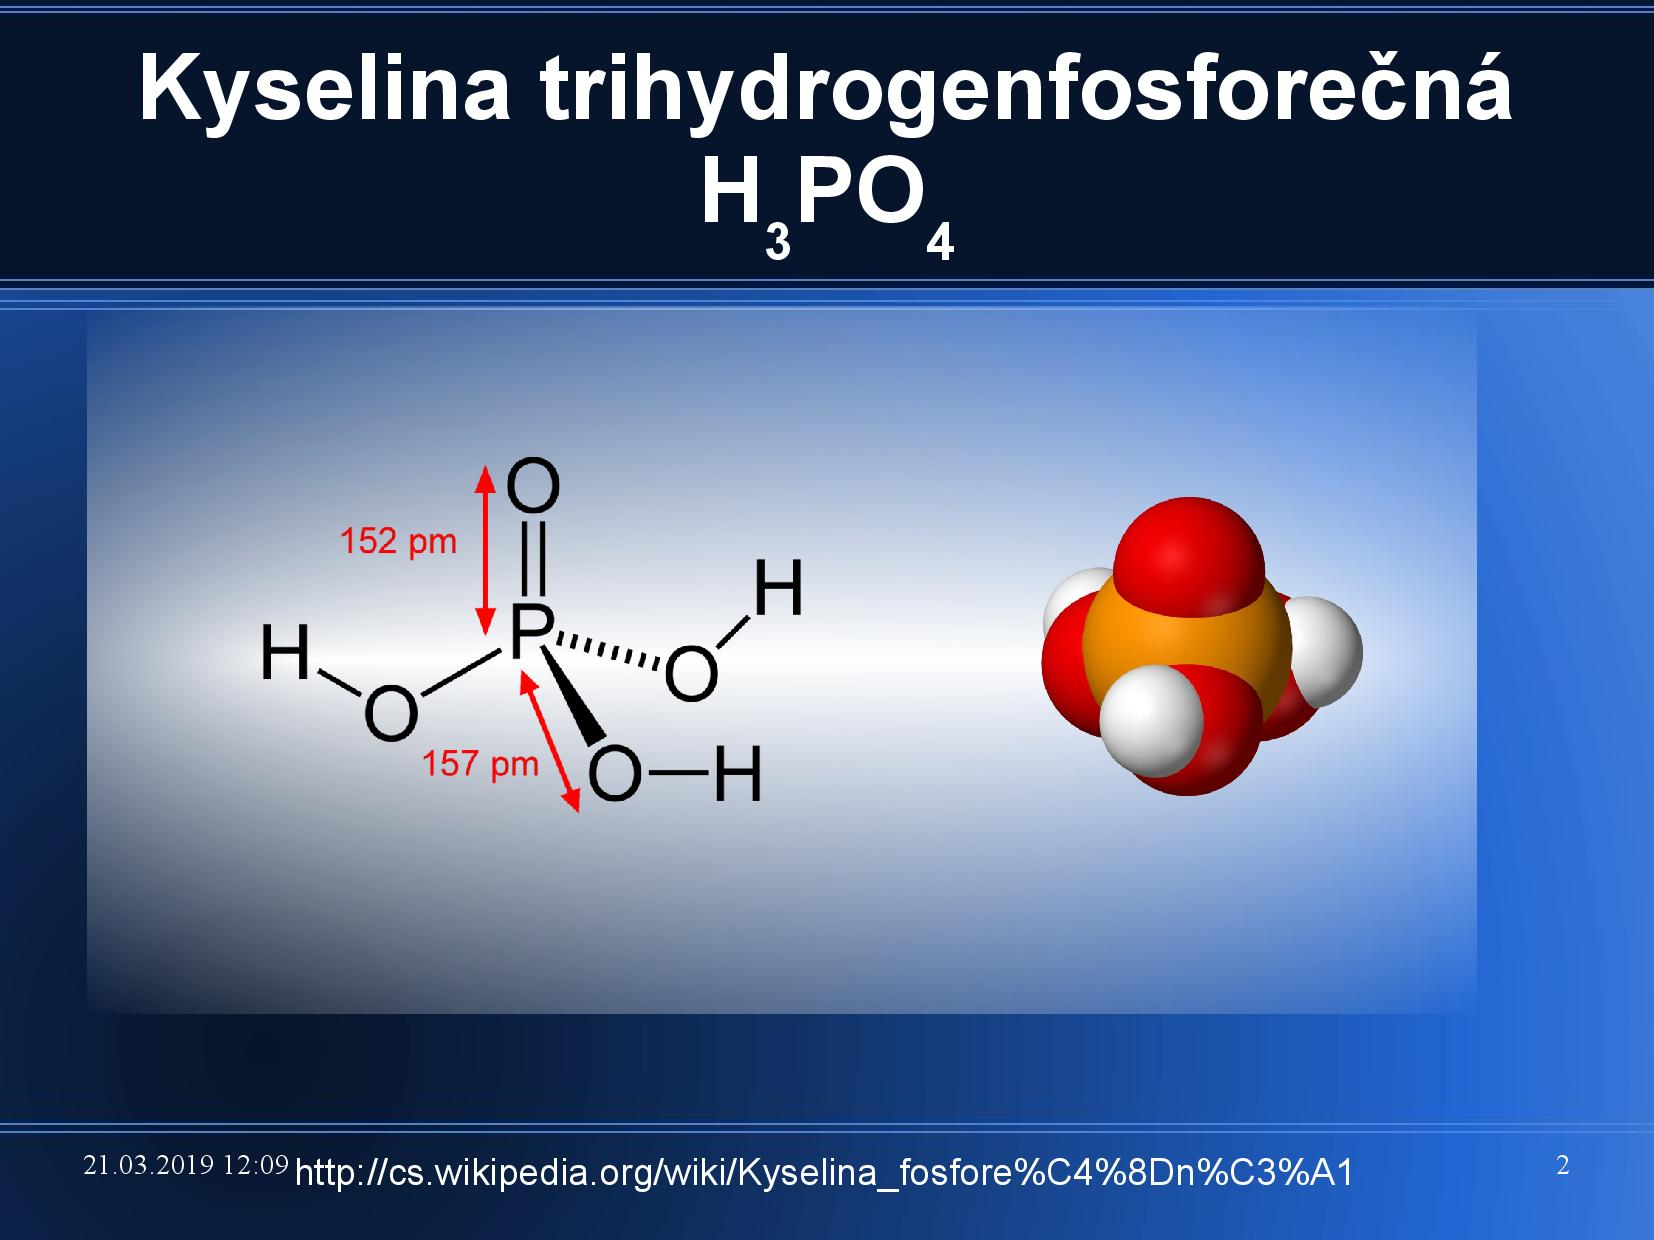
\includegraphics[width=0.85\textwidth]{slides-3/slide-2.jpg}
    \centering
    \label{slides-3-slide-2}
\end{figure}

\paragraph{Kyselina trihydrogen fosforečná}
\begin{itemize}[nosep]
    \item každý z vodíků může být disociován
    \item \(\ce{H3PO4}\) někdy tvoří dimer, \emph{pyrofosfát} \begin{figure}
    \caption{Prezentace č. 3, slide č. 3}
    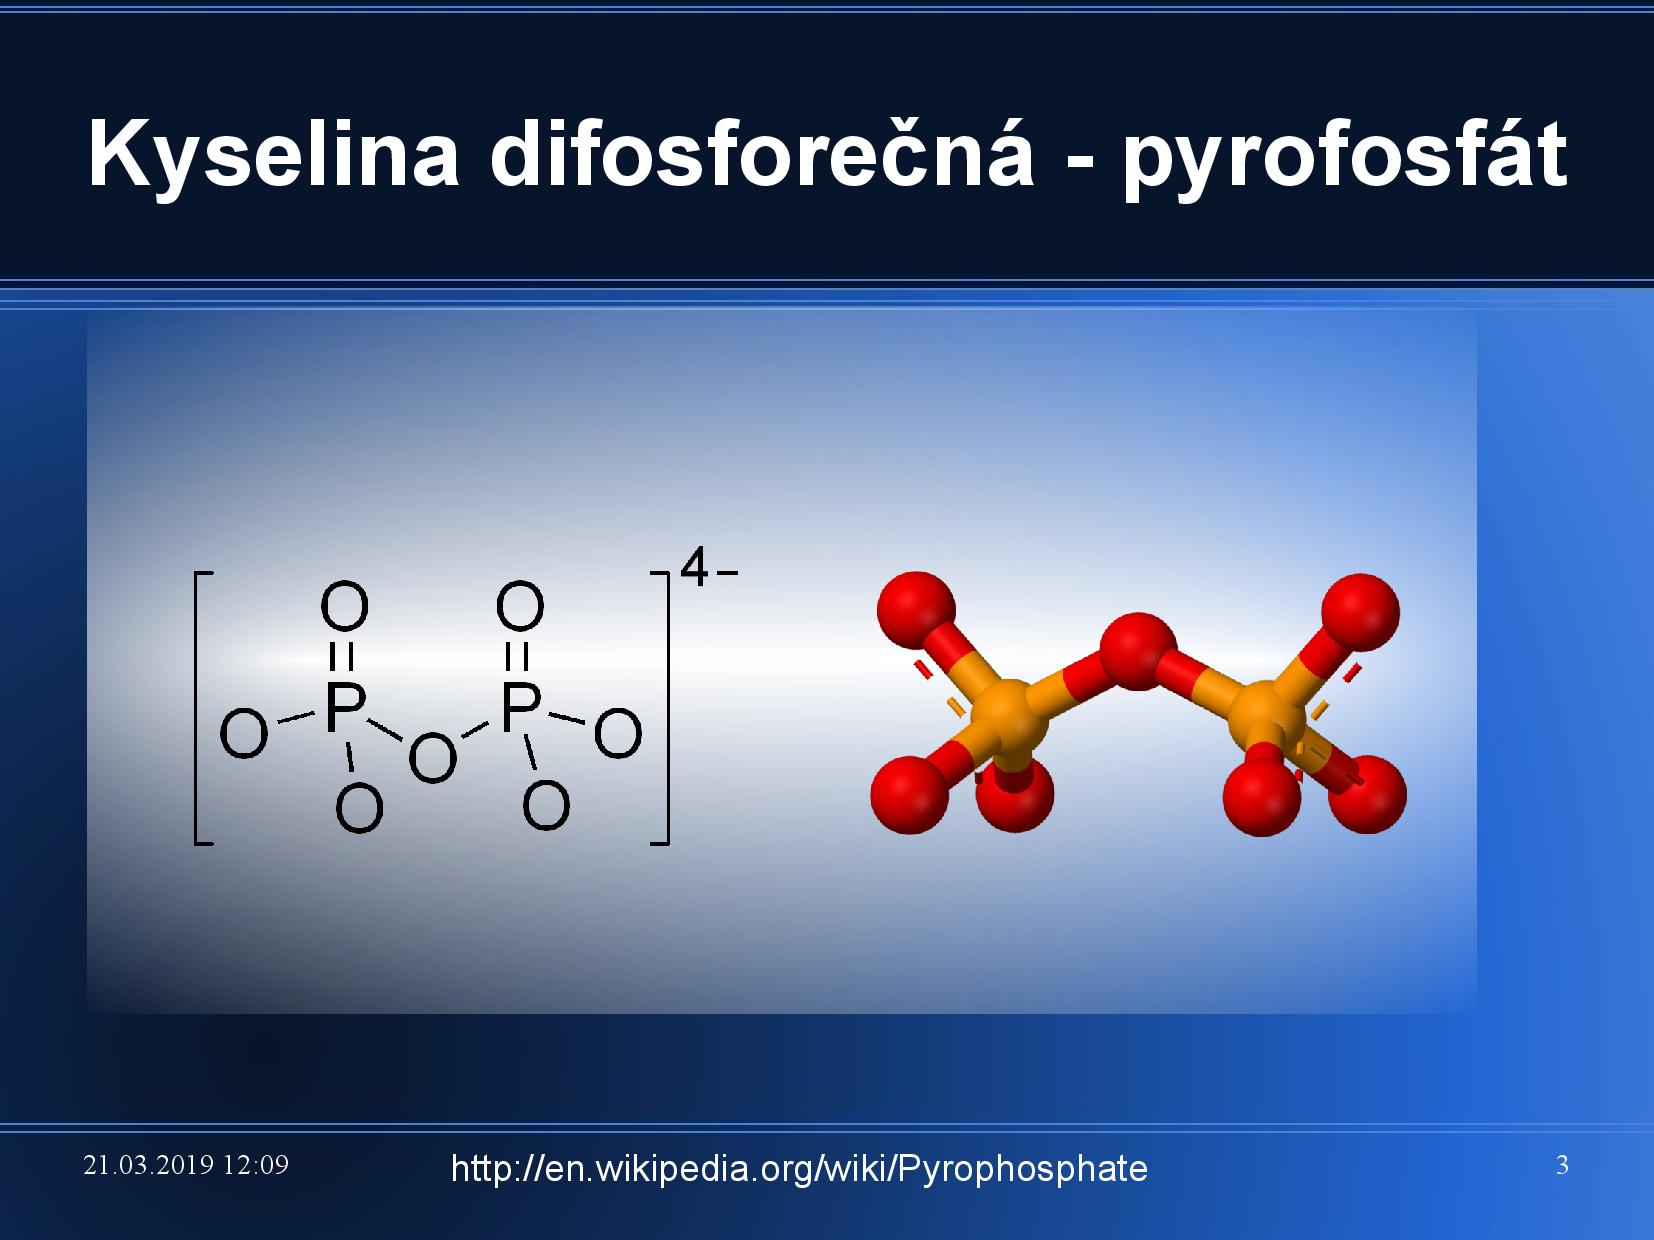
\includegraphics[width=0.85\textwidth]{slides-3/slide-3.jpg}
    \centering
    \label{slides-3-slide-3}
\end{figure}

\begin{itemize}[nosep]
    \item spojené makroergní vazbou (při rozštěpení se uvolní velké množtsví energie)
    \item makroergní proto, že jsou k sobě blízko kyslíky (vzniká mechanické pnutí)
\end{itemize}

    \item trifosforečná kyselina bývá vázána v nukleotidech
\end{itemize}




Základním cukrem je ribóza a deoxyribóza. Základní strukturní vlastnosti cukrů jsou však předvedeny na glukóze.

\mybox{TODO}{Doplnit, jak vypadá D-glukosa v cyklické formě.}


\begin{figure}
    \caption{Prezentace č. 3, slide č. 5}
    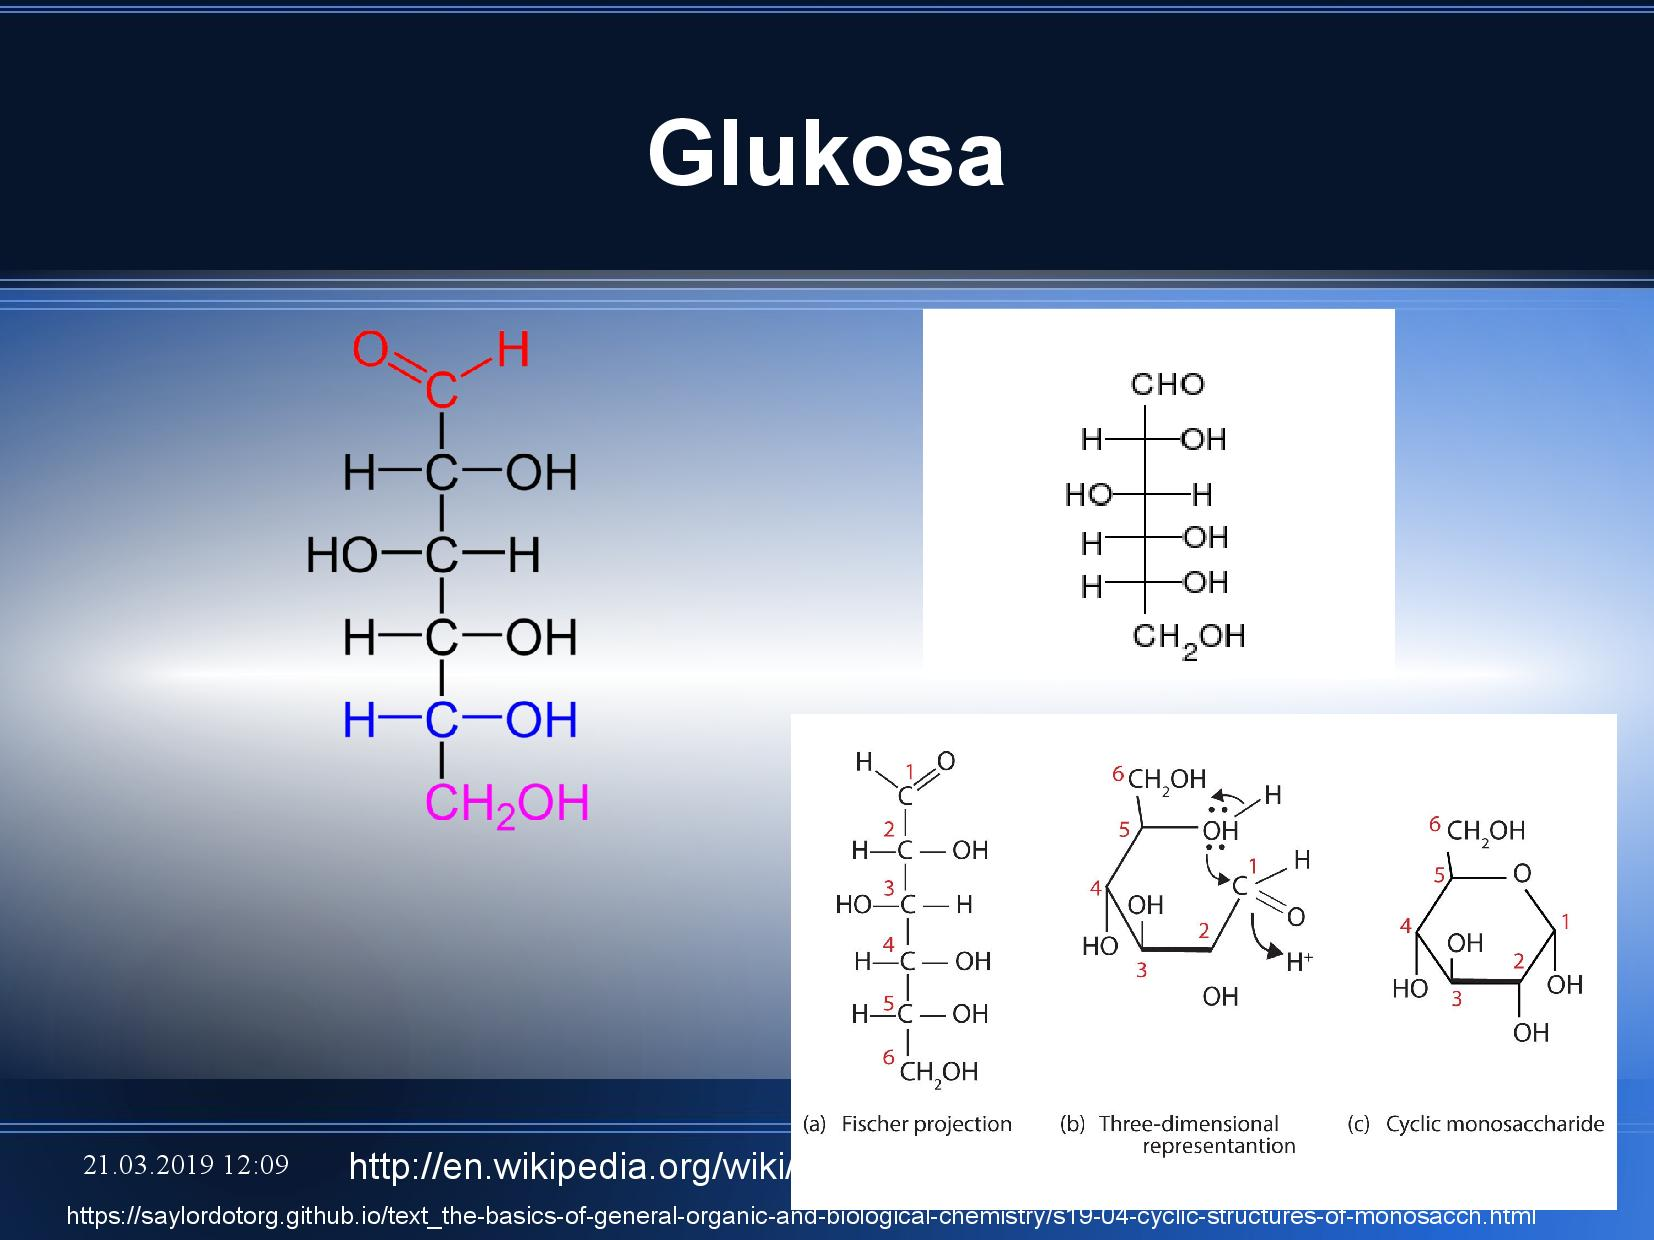
\includegraphics[width=0.85\textwidth]{slides-3/slide-5.jpg}
    \centering
    \label{slides-3-slide-5}
\end{figure}
\begin{figure}
    \caption{Prezentace č. 3, slide č. 6}
    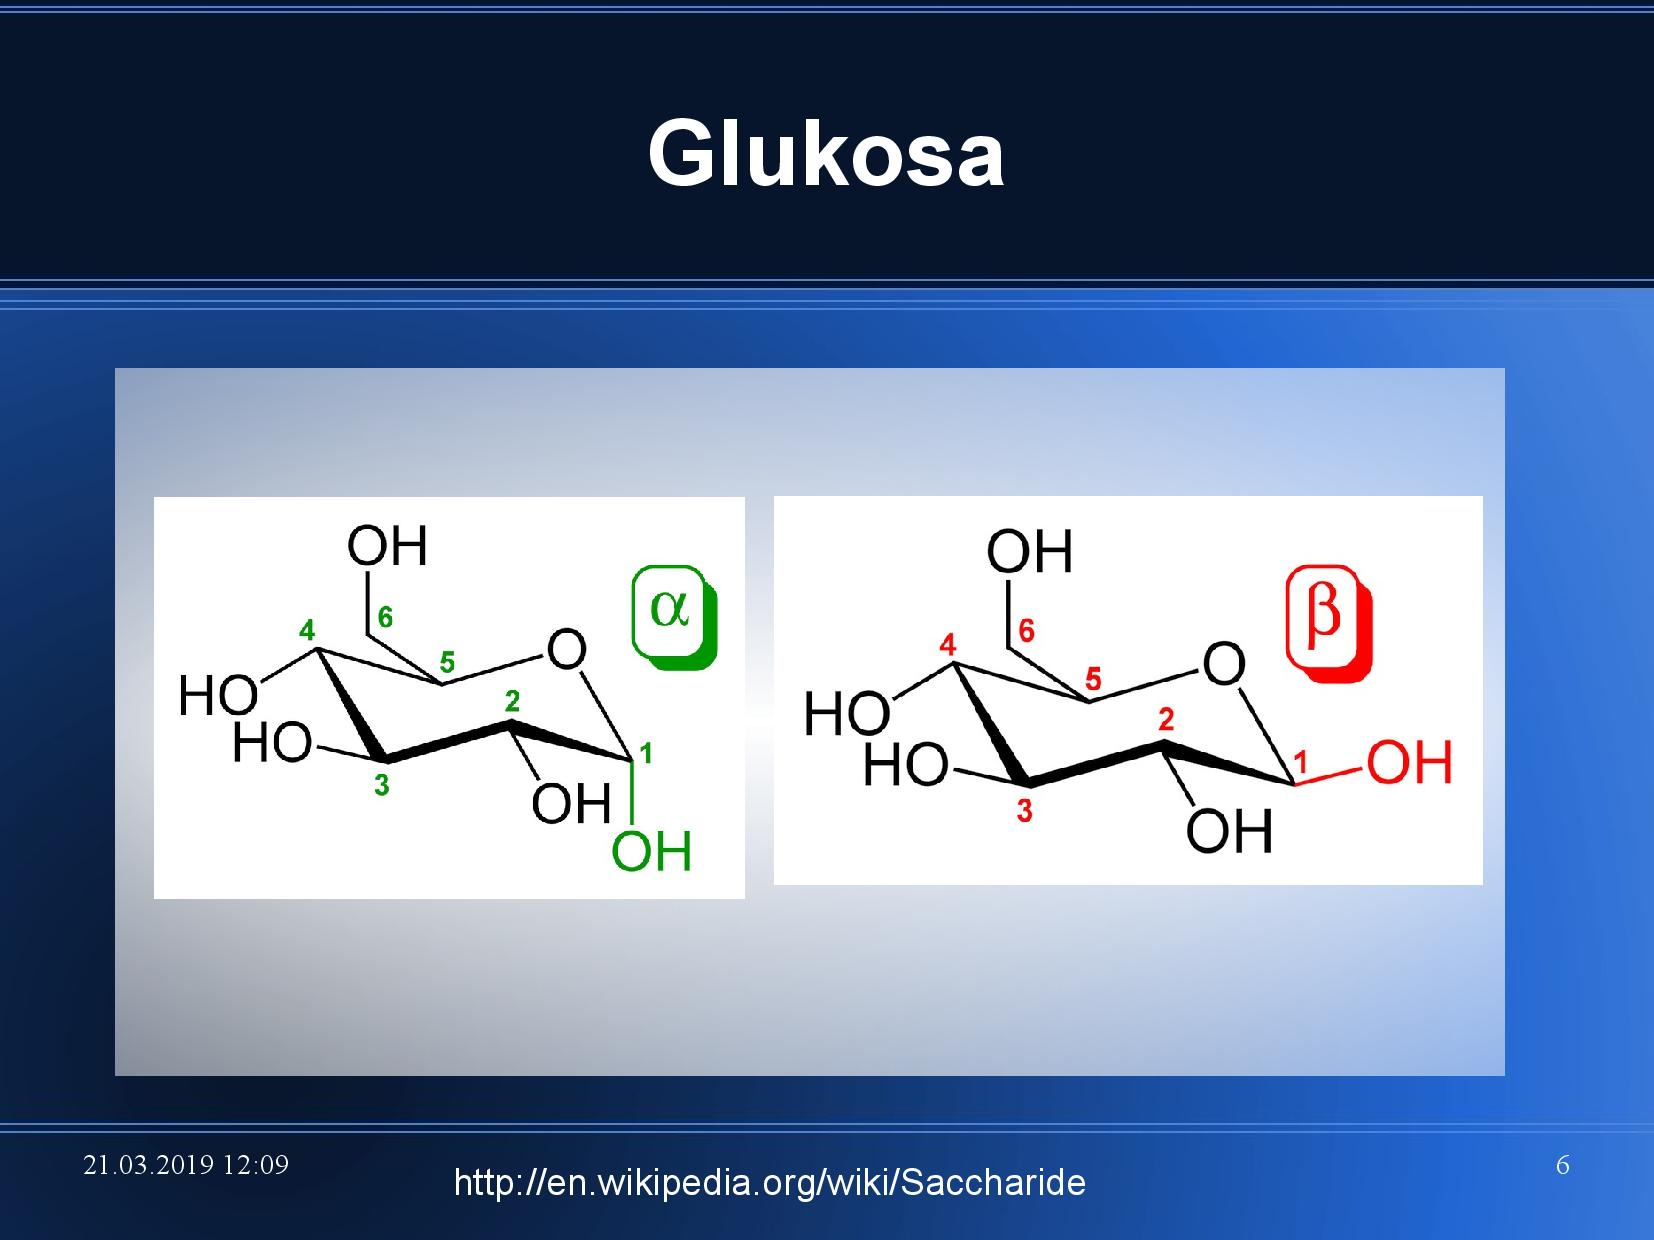
\includegraphics[width=0.85\textwidth]{slides-3/slide-6.jpg}
    \centering
    \label{slides-3-slide-6}
\end{figure}

\paragraph{Glukóza}
\begin{itemize}[nosep]
    \item pojmenování podle polohy OH skupiny na chirálním uhlíku, který je nejvzdálenější od aldehydické skupiny
\begin{itemize}[nosep]
    \item v lineárním Fisherově zakreslení: OH vpravo -> D-forma, OH vlevo -> L-forma
\end{itemize}

    \item pokud dojde k vytvoření cukerného heterocyklu, můžeme rozlišit dvě formy podle polohy OH na \(\ce{C1}\)
\begin{itemize}[nosep]
    \item \(\alpha\), OH míří dolů
    \item \(\beta\), OH míří nahoru
\end{itemize}

\end{itemize}



\begin{figure}
    \caption{Prezentace č. 3, slide č. 8}
    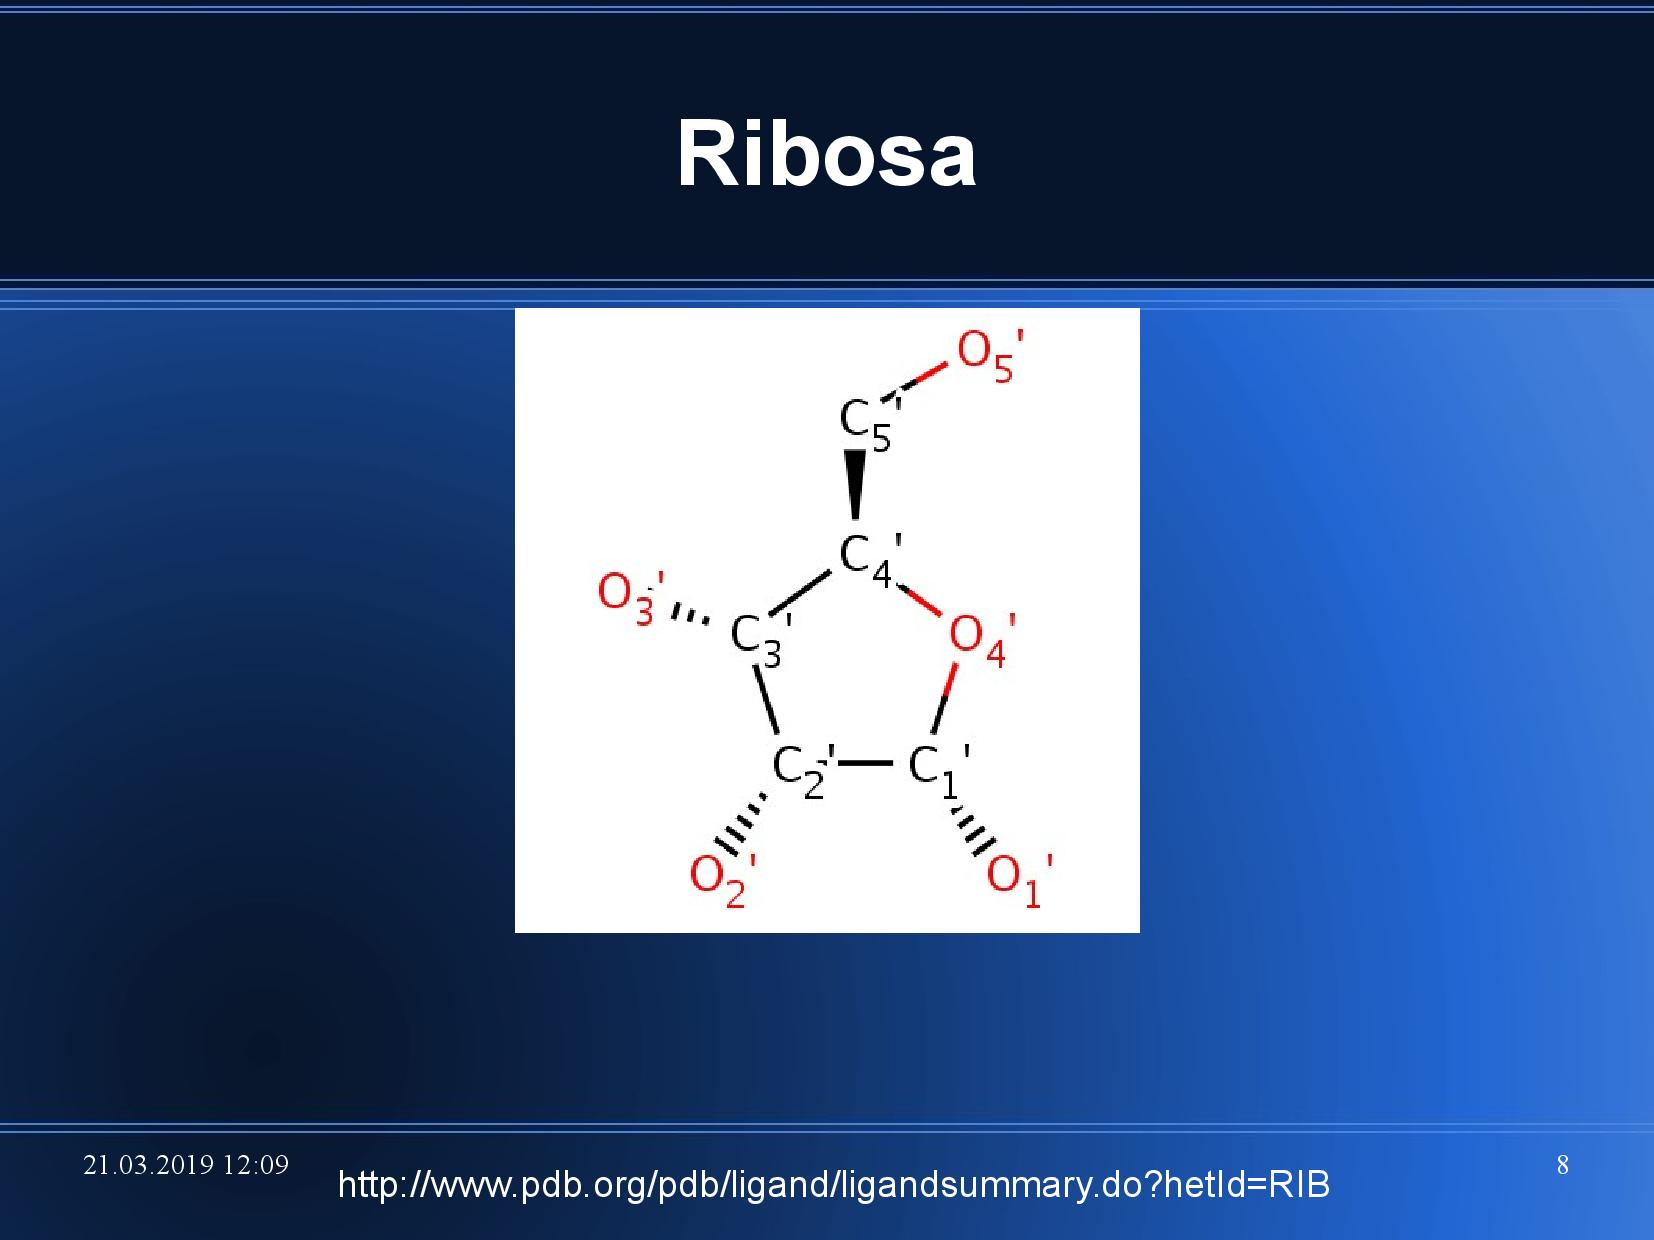
\includegraphics[width=0.85\textwidth]{slides-3/slide-8.jpg}
    \centering
    \label{slides-3-slide-8}
\end{figure}
\begin{figure}
    \caption{Prezentace č. 3, slide č. 9}
    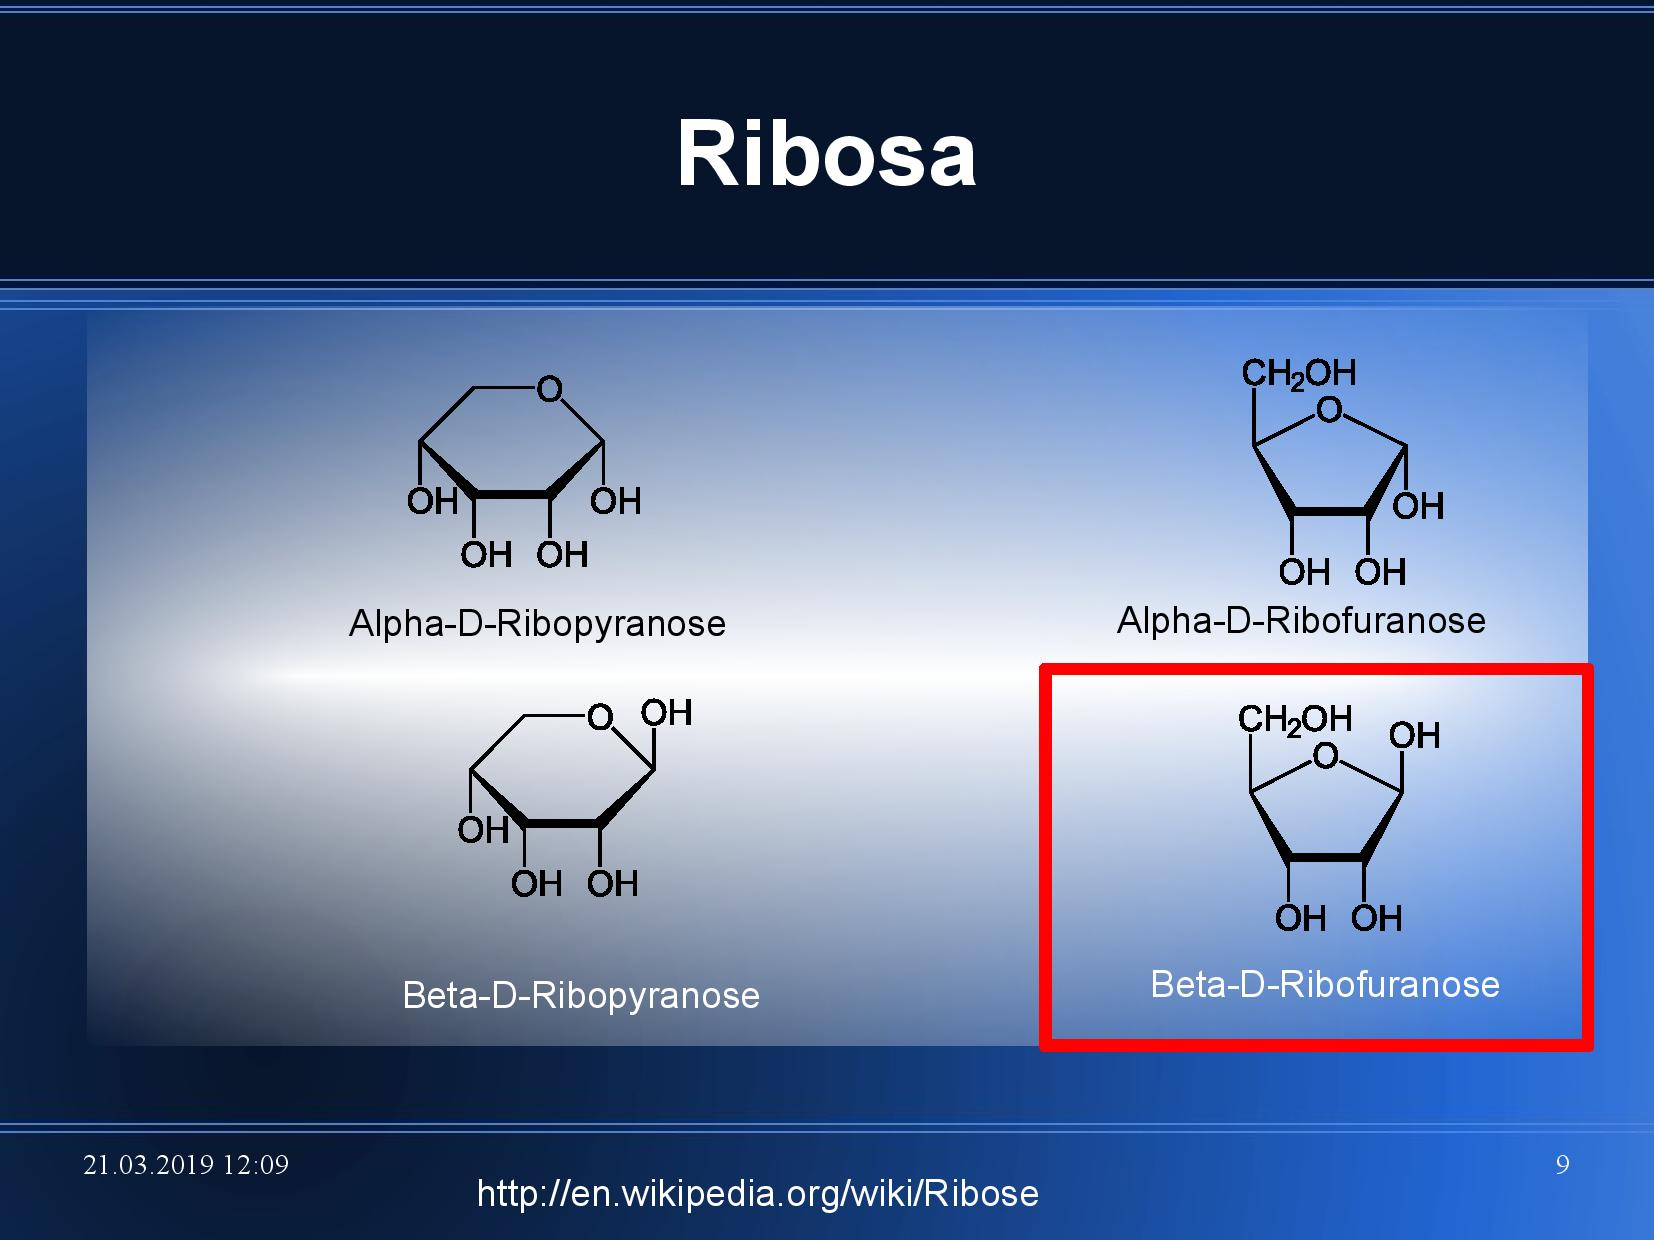
\includegraphics[width=0.85\textwidth]{slides-3/slide-9.jpg}
    \centering
    \label{slides-3-slide-9}
\end{figure}

\paragraph{Ribóza}
\begin{itemize}[nosep]
    \item v NA cyklizuje do pětičetného cyklu (ribofuranóza), může ale tvořit i šestičetný cyklus (ribopyranóza)
    \item uhlíky se v rámci NA značí s čarou
\begin{itemize}[nosep]
    \item fosfát je v NA vázaný na \(\ce{C3}\) a \(\ce{C5}\)
    \item na \(\ce{C1}\) je přes N-glykosidickou vazbu navázána dusíkatá báze
    \item na \(\ce{C2}\) je OH skupina (RNA), případně tam není (DNA)
\end{itemize}

    \item celkově je tedy v NA (případně deoxy verze)
    \item cyklus \textbf{není planární} \begin{figure}
    \caption{Prezentace č. 3, slide č. 10}
    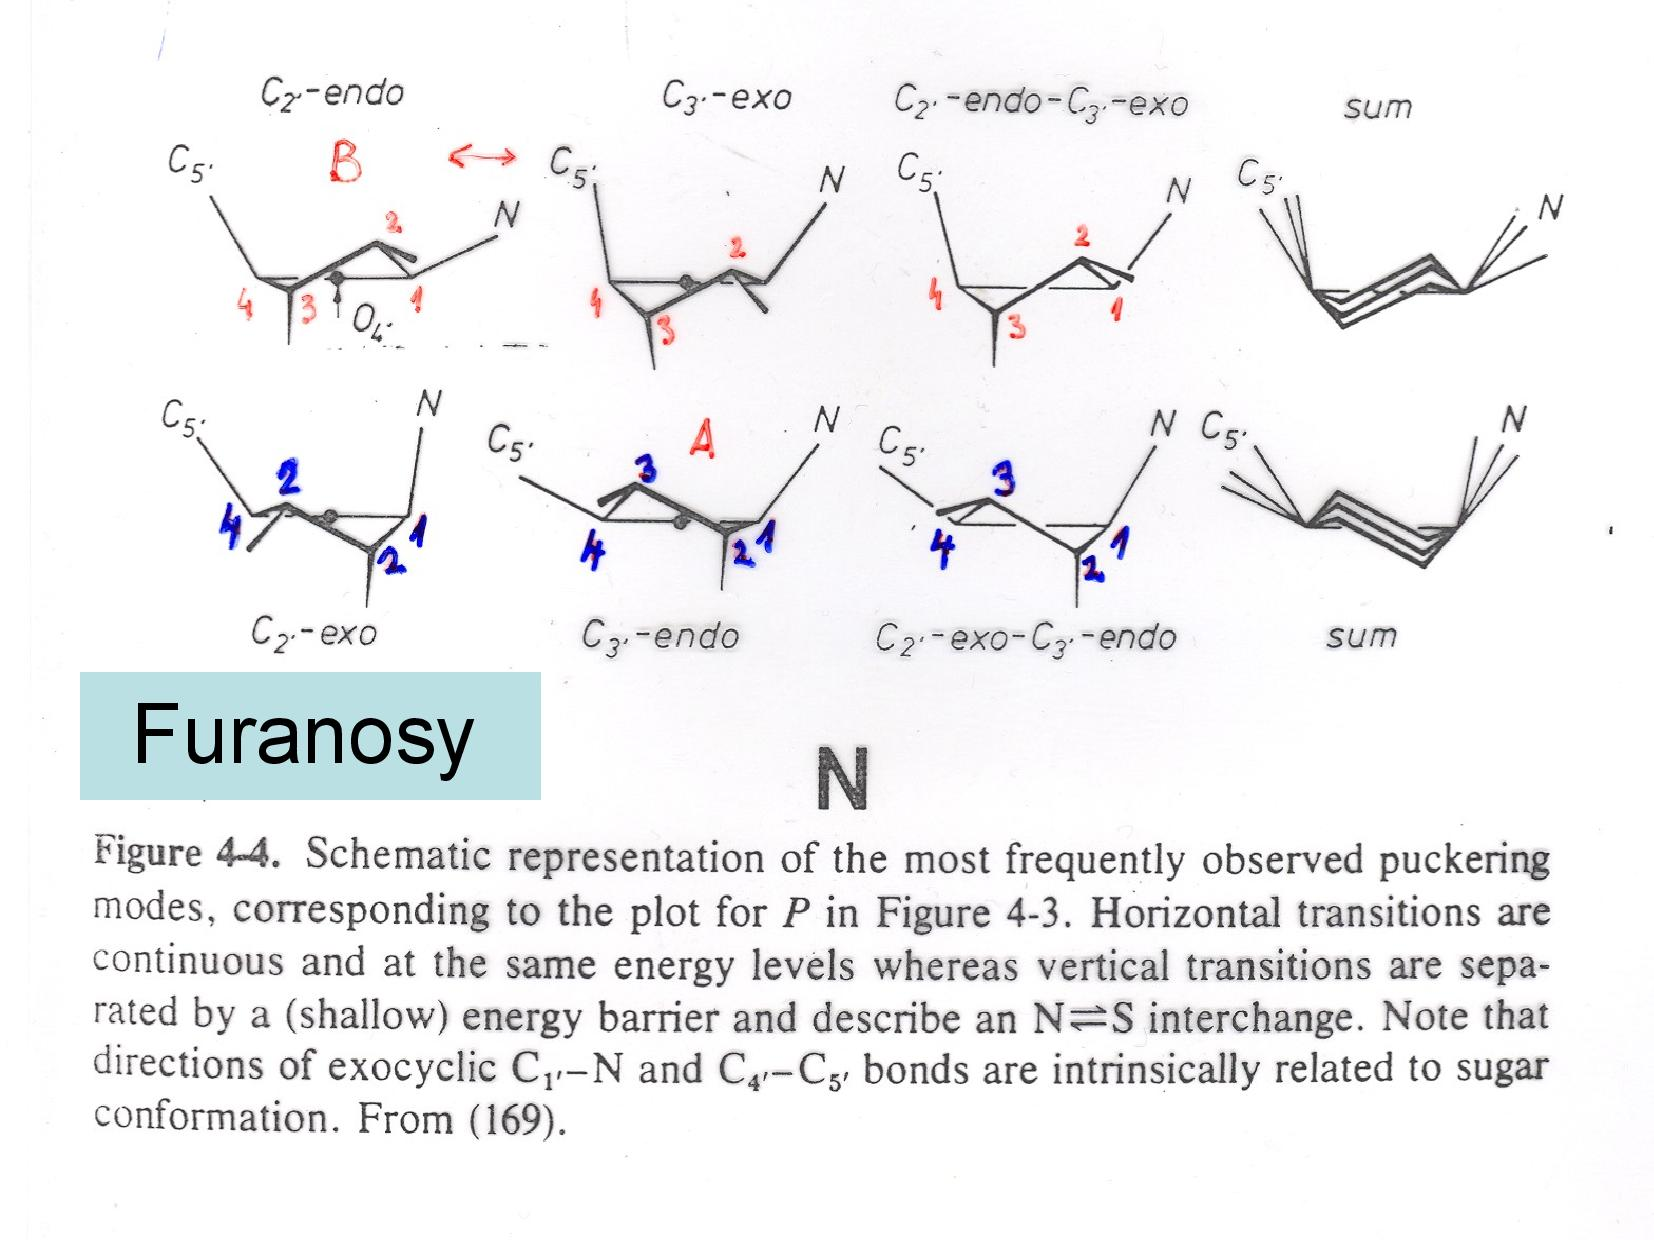
\includegraphics[width=0.85\textwidth]{slides-3/slide-10.jpg}
    \centering
    \label{slides-3-slide-10}
\end{figure}

\begin{itemize}[nosep]
    \item pokud \(\ce{C2}\) míří na stejnou stranu jako \(\ce{C5}\), je NA takzvaně \emph{endo} (případně C2 endo)
    -pokud míří \(\ce{C2}\) na opačnou stranu, je NA \emph{exo} (případně C2 exo)
\end{itemize}

\end{itemize}



\begin{figure}
    \caption{Prezentace č. 3, slide č. 12}
    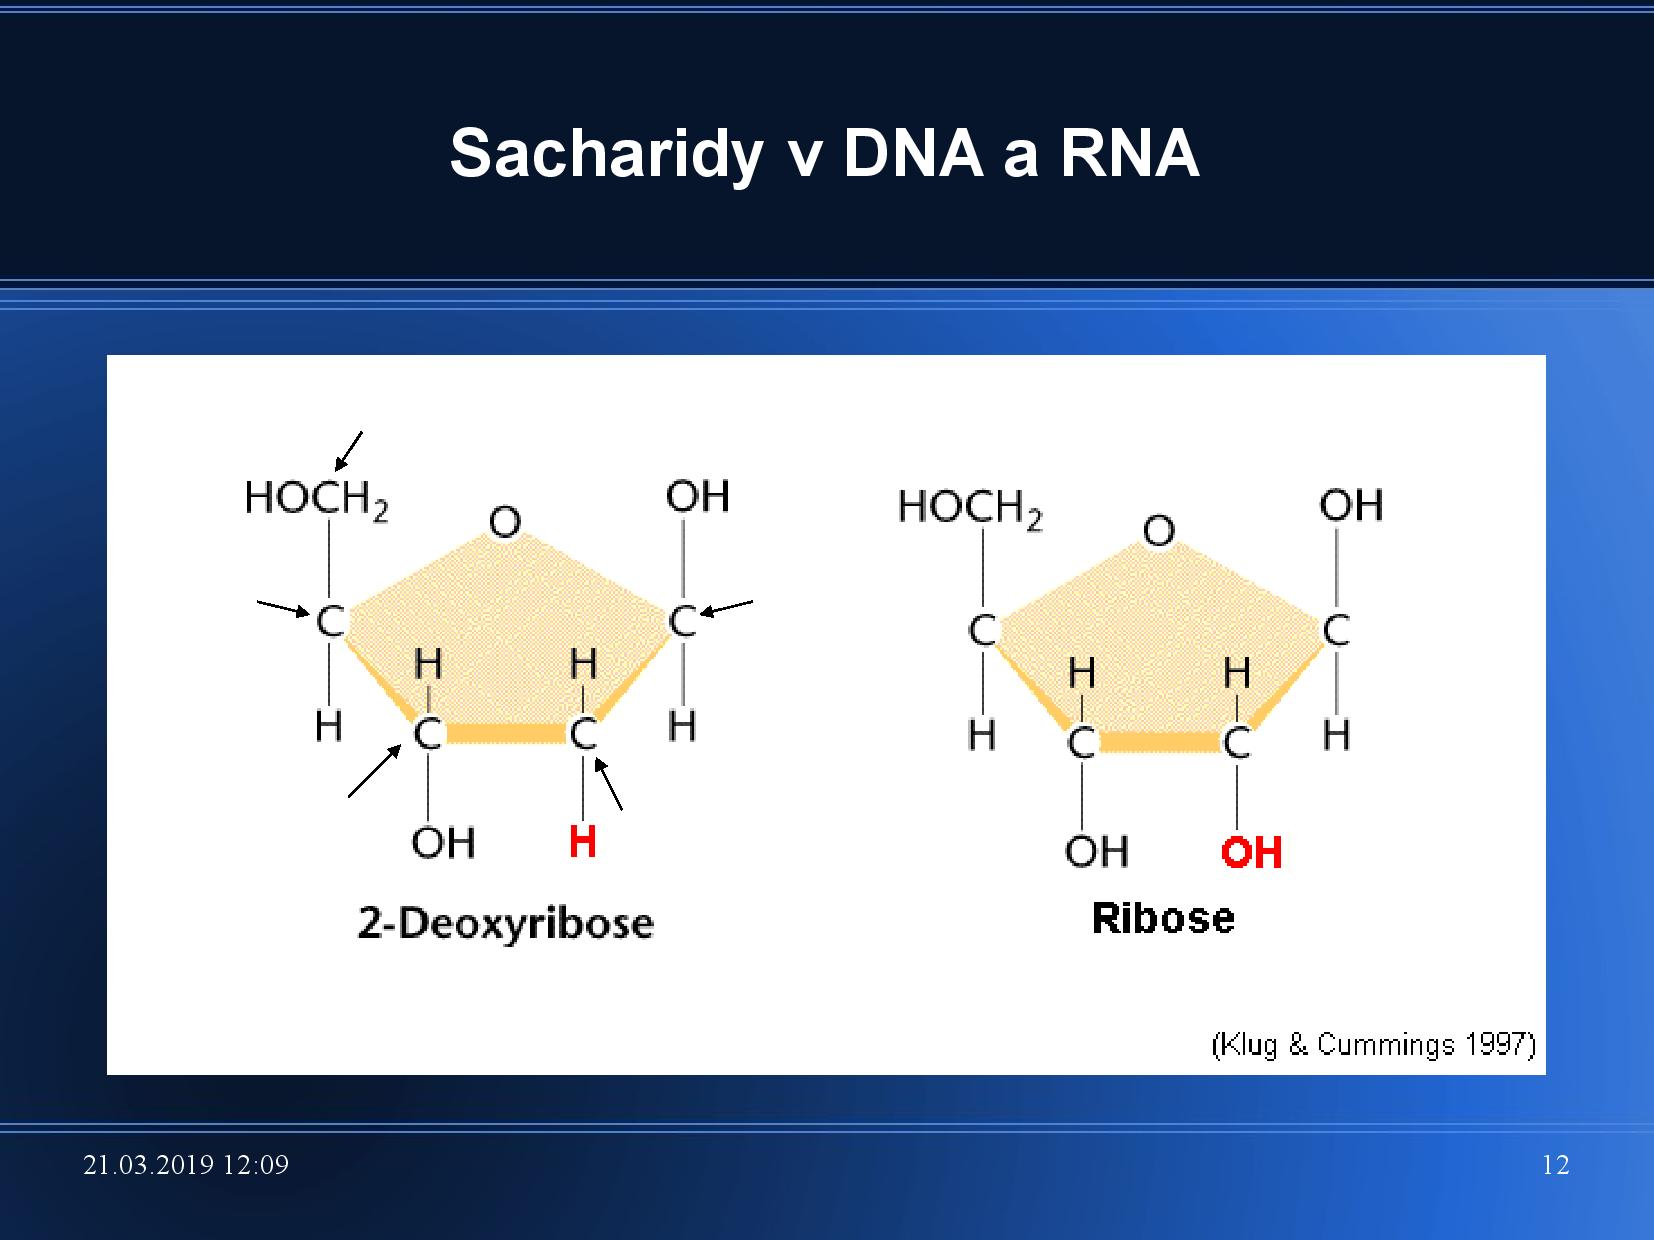
\includegraphics[width=0.85\textwidth]{slides-3/slide-12.jpg}
    \centering
    \label{slides-3-slide-12}
\end{figure}

V NA tedy nacházíme \textbf{\(\beta\)-D-ribofuranózu}, a to buďto endo nebo exo formu. Samozřejmě v DNA je deoxy- varianta tohoto cuktu, viz slide. OH skupina má vliv na reaktivitu, DNA je proto mnohem stabilnější než RNA.

Cukr s fosfátem (navázaným přes fosfodiesterovou vazbu) tvoří tzv. \emph{cukrfosfátovou kostru} NA.

\begin{figure}
    \caption{Dusíkaté báze nukleových kyselin}
    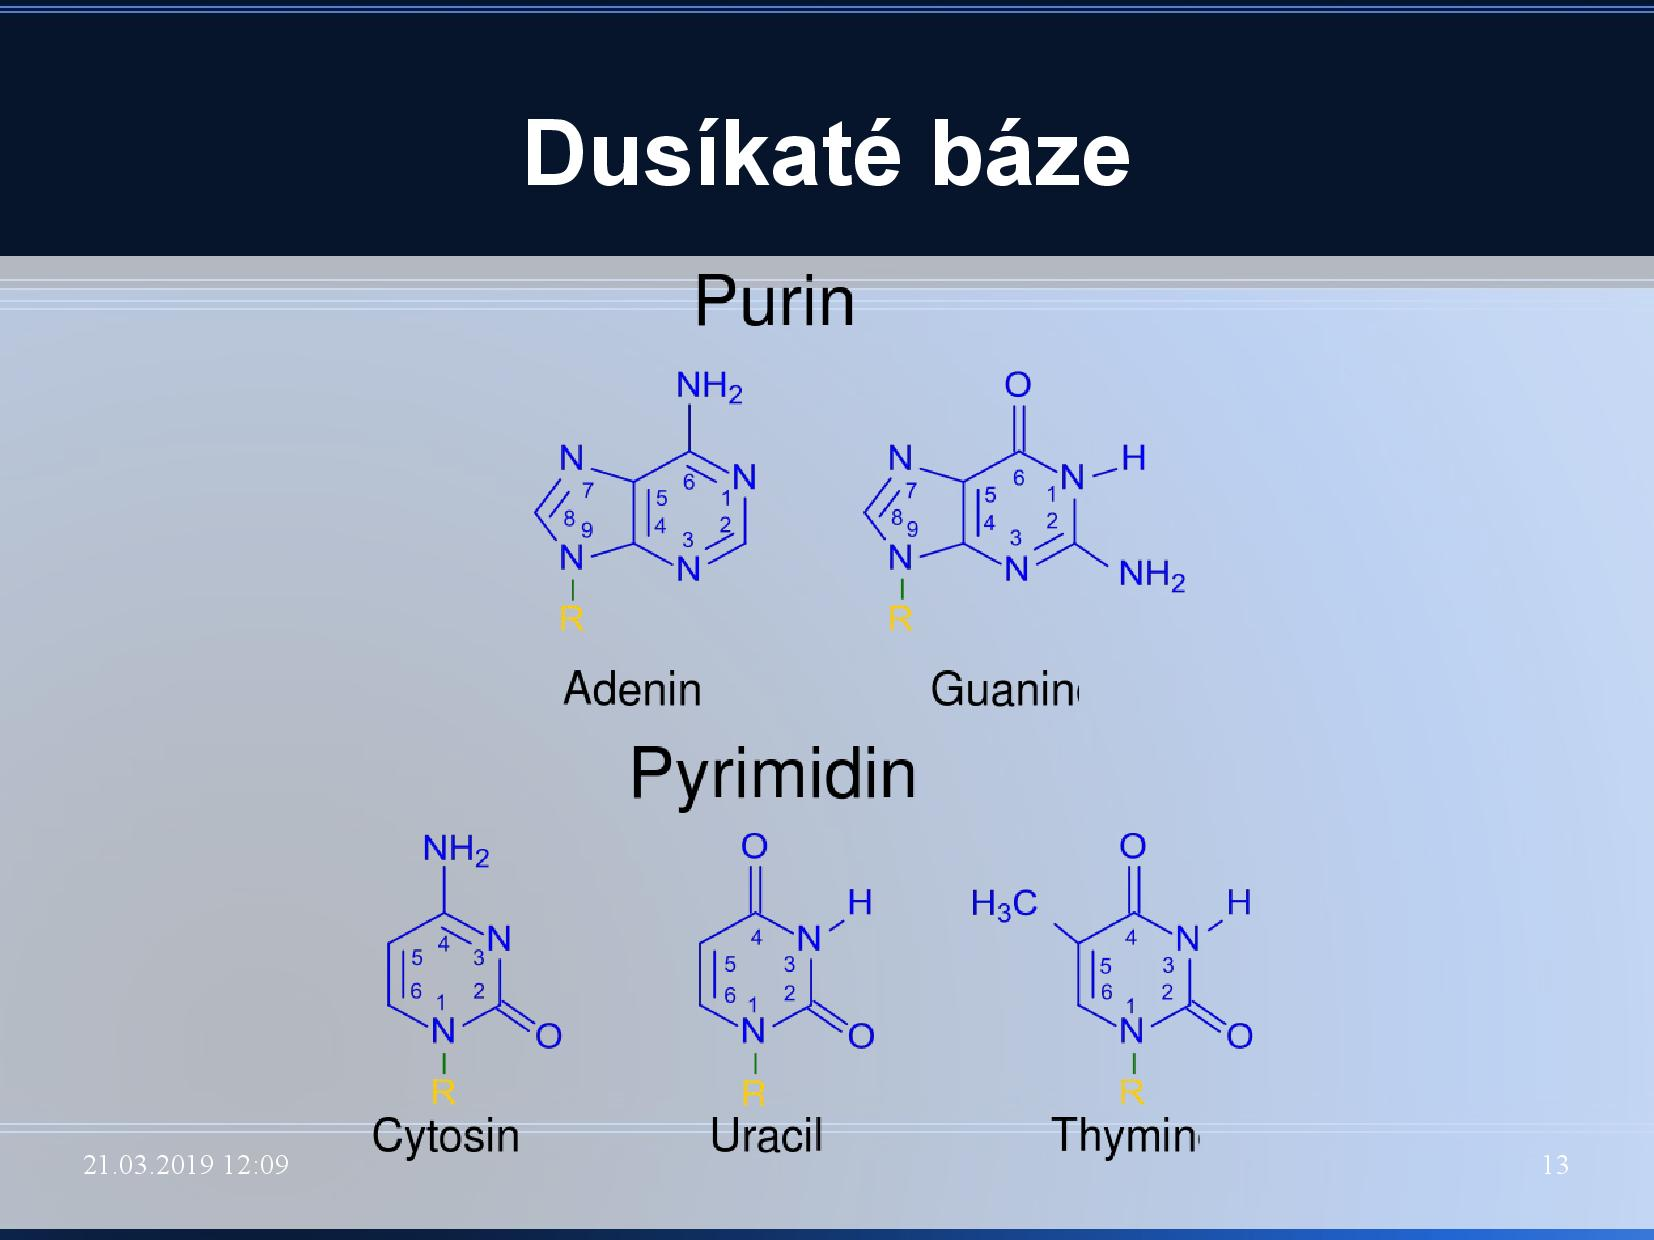
\includegraphics[width=0.85\textwidth]{slides-3/slide-13.jpg}
    \centering
    \label{}
\end{figure}


\paragraph{Dusíkaté báze}
\begin{itemize}[nosep]
    \item puriny jsou na \(\ce{C1}\) v cukru vázány dusíkem \(\ce{N9}\), pyrimidiny dusíkem \(\ce{N1}\)
\begin{itemize}[nosep]
    \item puriny jsou vlastně kondenzáty pyrimidinu a imidazolu
\end{itemize}

    \item Watson-Crickovo párování: párování GC, AT, na základě vodíkových můstků \begin{figure}
    \caption{Prezentace č. 3, slide č. 13}
    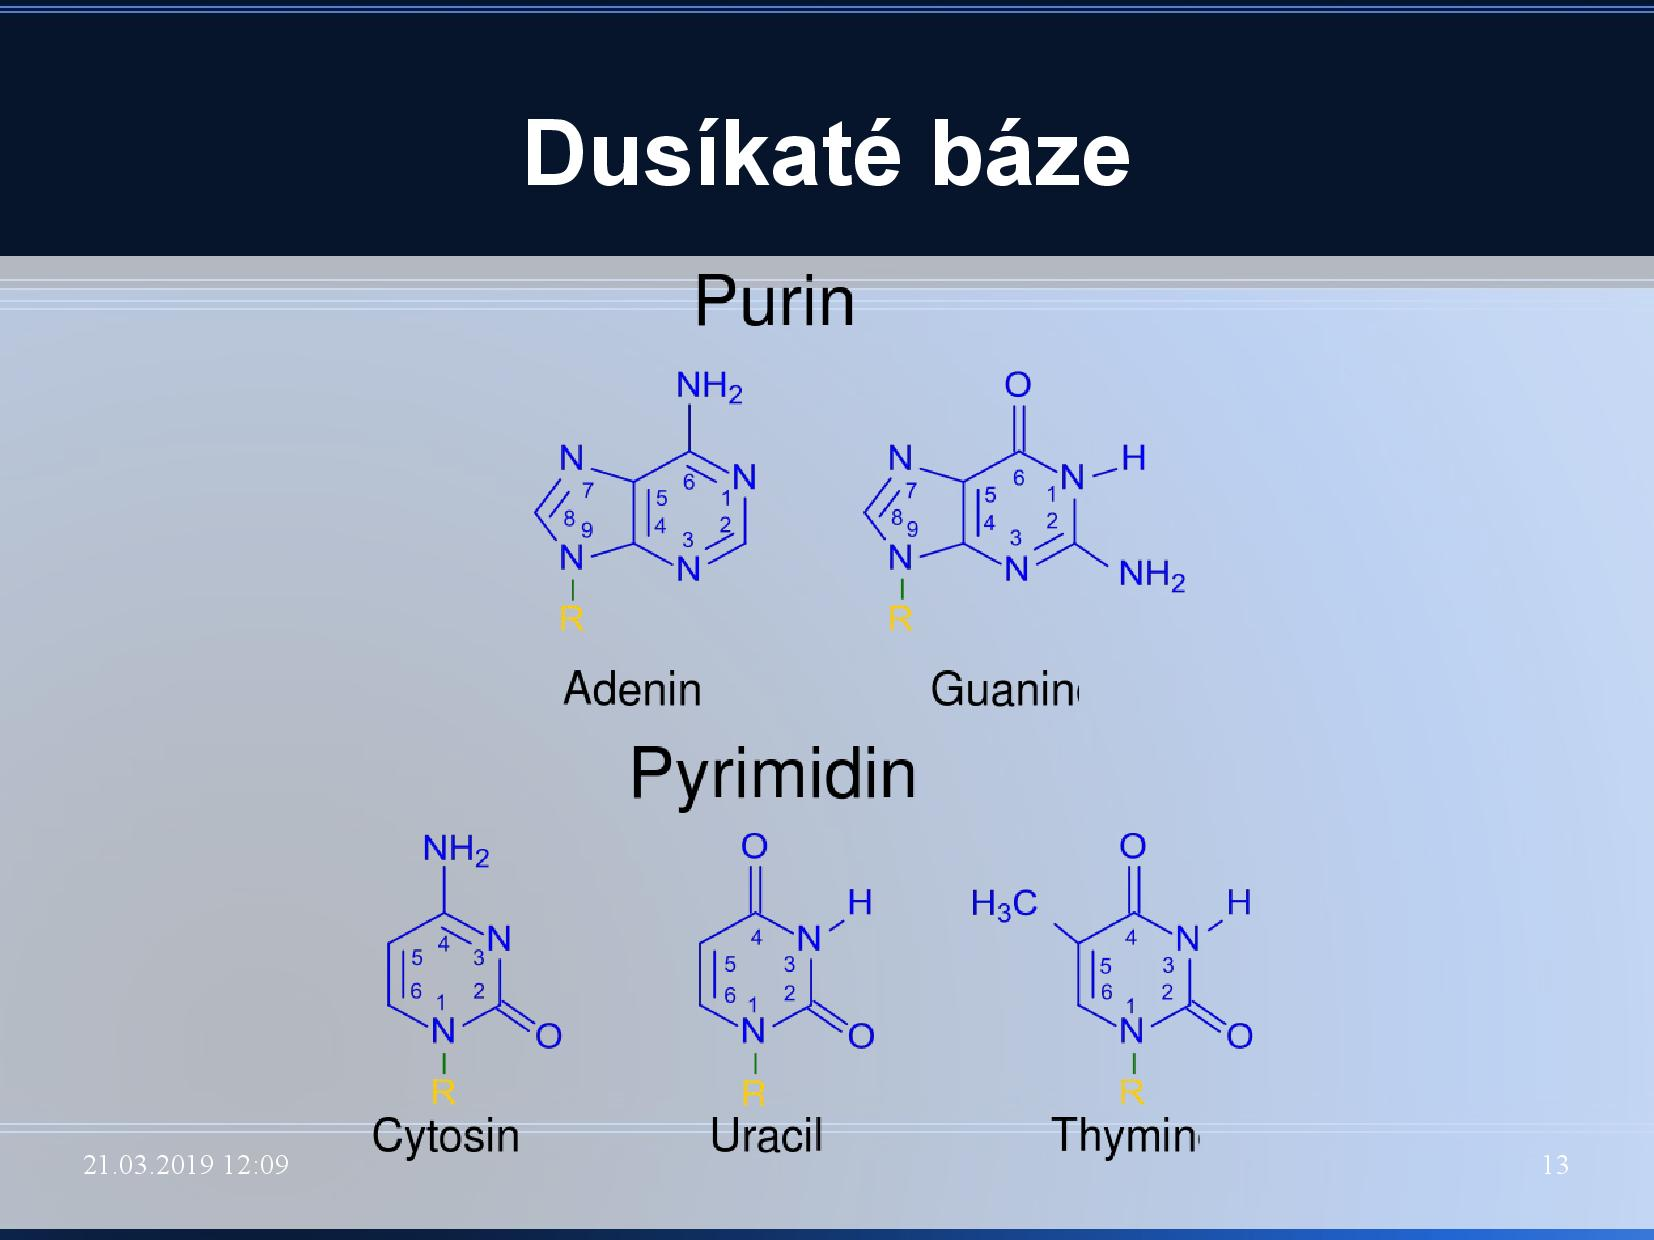
\includegraphics[width=0.85\textwidth]{slides-3/slide-13.jpg}
    \centering
    \label{slides-3-slide-13}
\end{figure}

    \item v DNA je nahrazen thymin uracilem (který se liší jen jednou metylovou skupinou)
    \item kromě těchto základních se vyskytují v DNA i další, minoritní, báze: methylované báze a hydroxymethylované báze, uracil
    \item uracil má někdy tvar pseudouridinu, dihydrouridinu atp. \begin{figure}
    \caption{Prezentace č. 3, slide č. 37}
    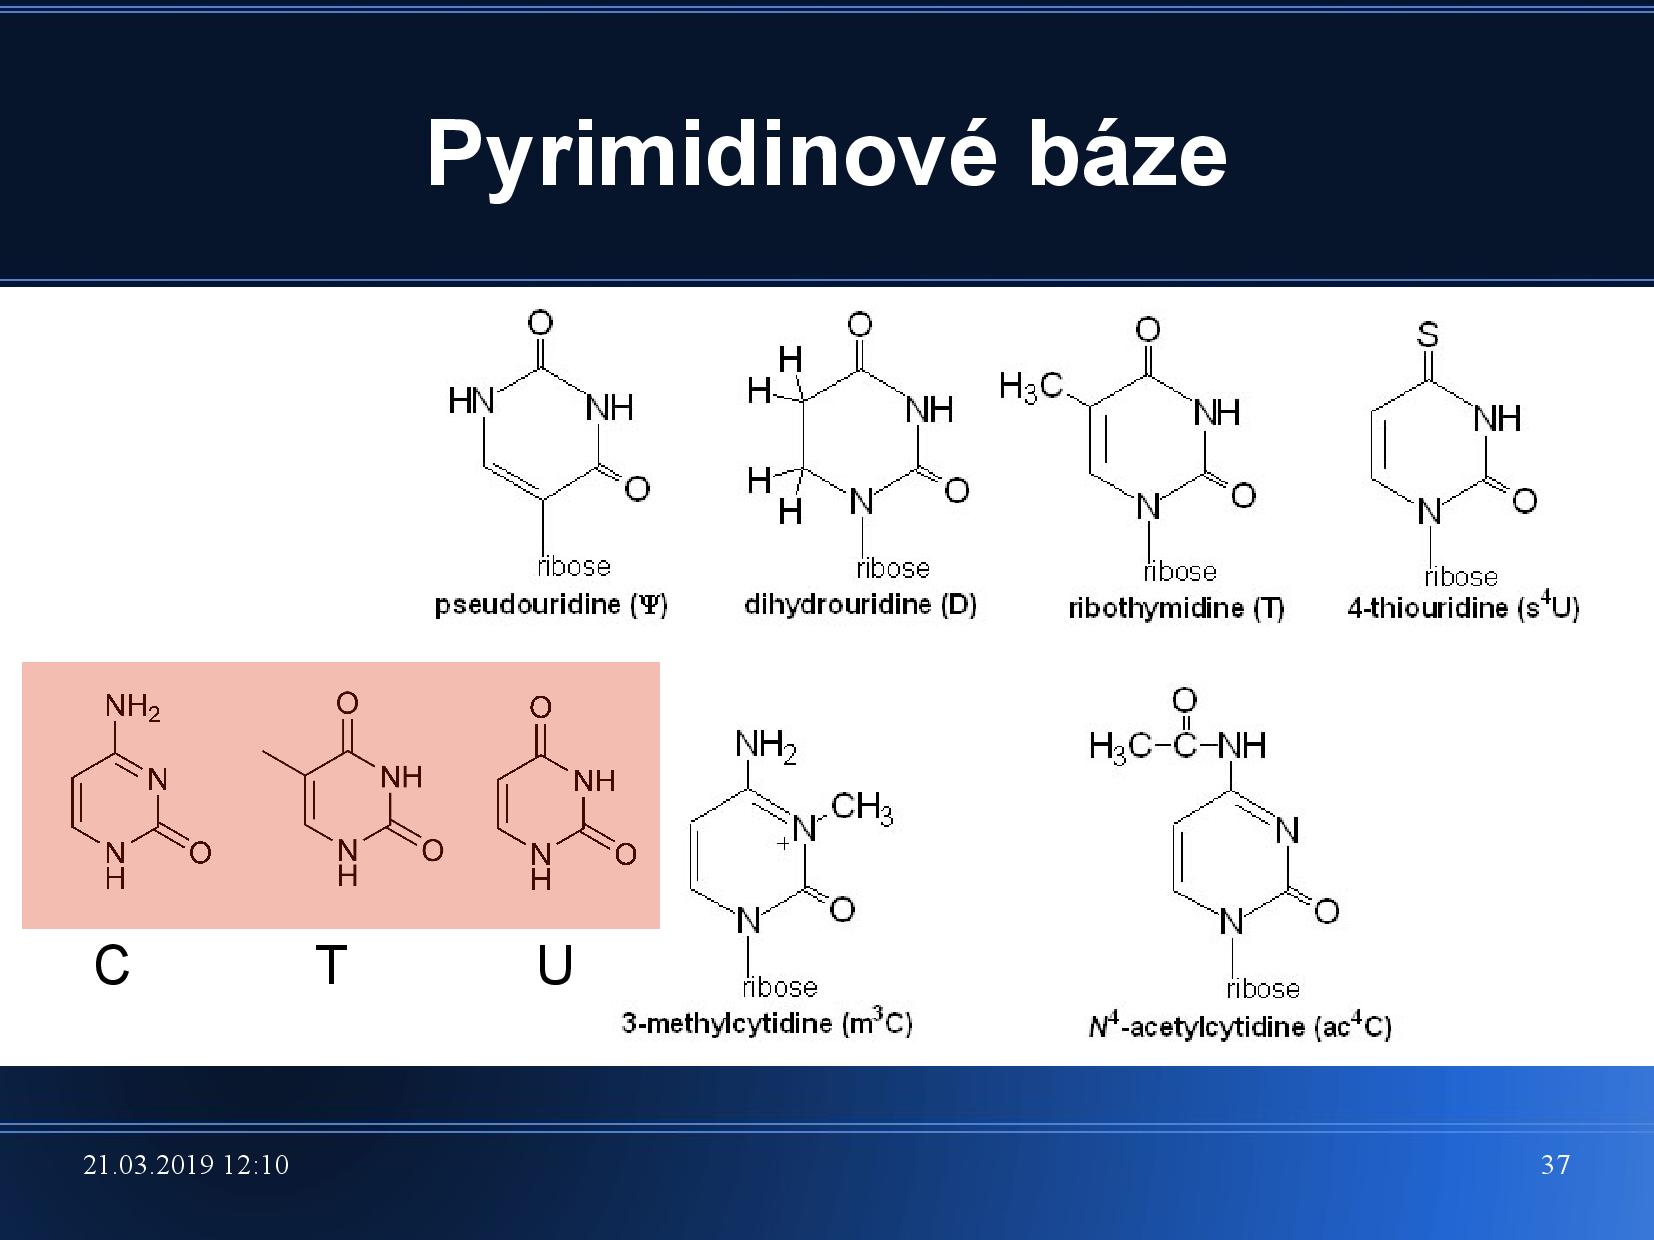
\includegraphics[width=0.85\textwidth]{slides-3/slide-37.jpg}
    \centering
    \label{slides-3-slide-37}
\end{figure}

    \item jeden pár bazí má asi 660g/mol, neboli 660Da
\end{itemize}



\paragraph{Párování bazí}
\begin{itemize}[nosep]
    \item keto skupina je vždy akceptor
    \item amino skupina vždy donor
    \item sekundární amin, imin: mohou fungovat jako akceptor
\end{itemize}



\section{Struktura} \label{Struktura}


\begin{figure}
    \caption{Prezentace č. 3, slide č. 16}
    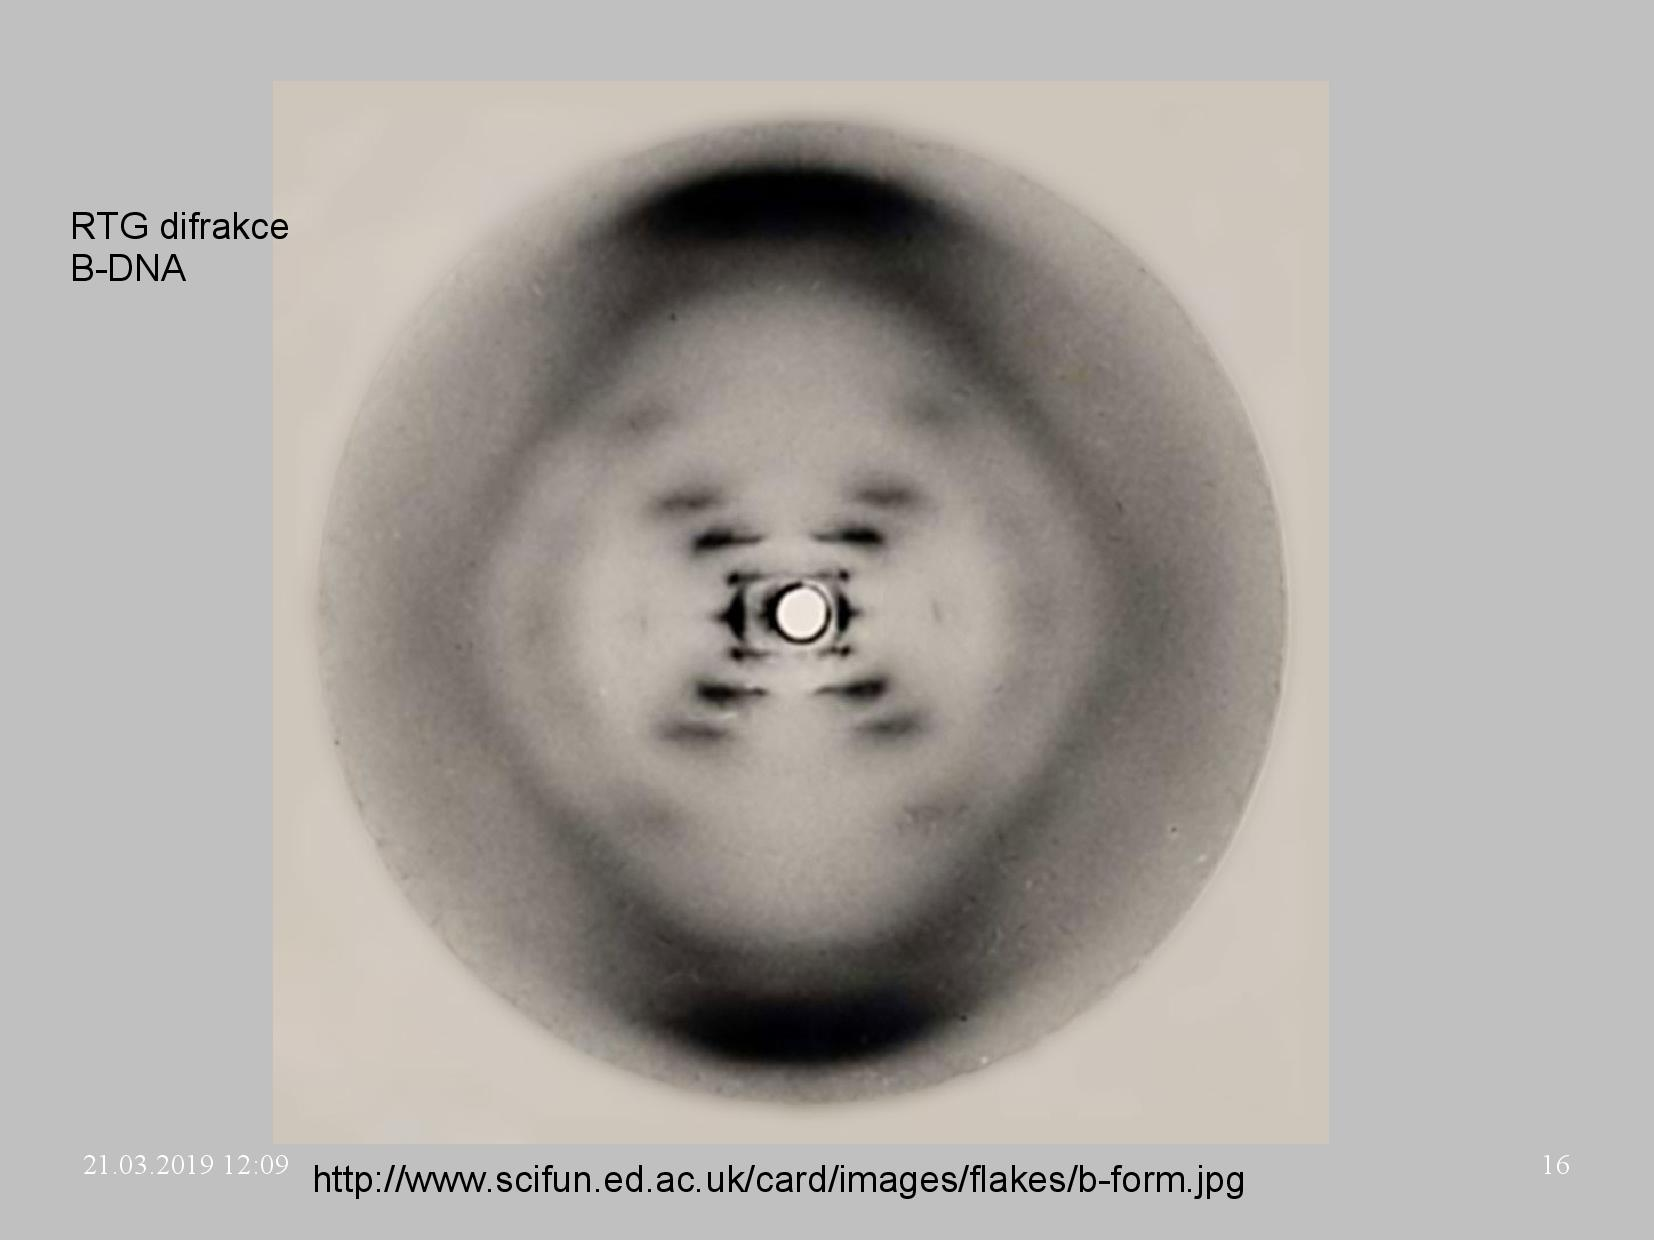
\includegraphics[width=0.85\textwidth]{slides-3/slide-16.jpg}
    \centering
    \label{slides-3-slide-16}
\end{figure}

\begin{itemize}[nosep]
    \item vlákna v DNA jsou antiparalelní, jedno je ve směru 3'->5' a druhé 5'->3'
    \item zaujímají strukturu dihelixu (Watson, Crick)
\begin{itemize}[nosep]
    \item difrakční obrazec spirály má tvar X
\end{itemize}

\end{itemize}



\begin{figure}
    \caption{Nukleosid, nukleotid}
    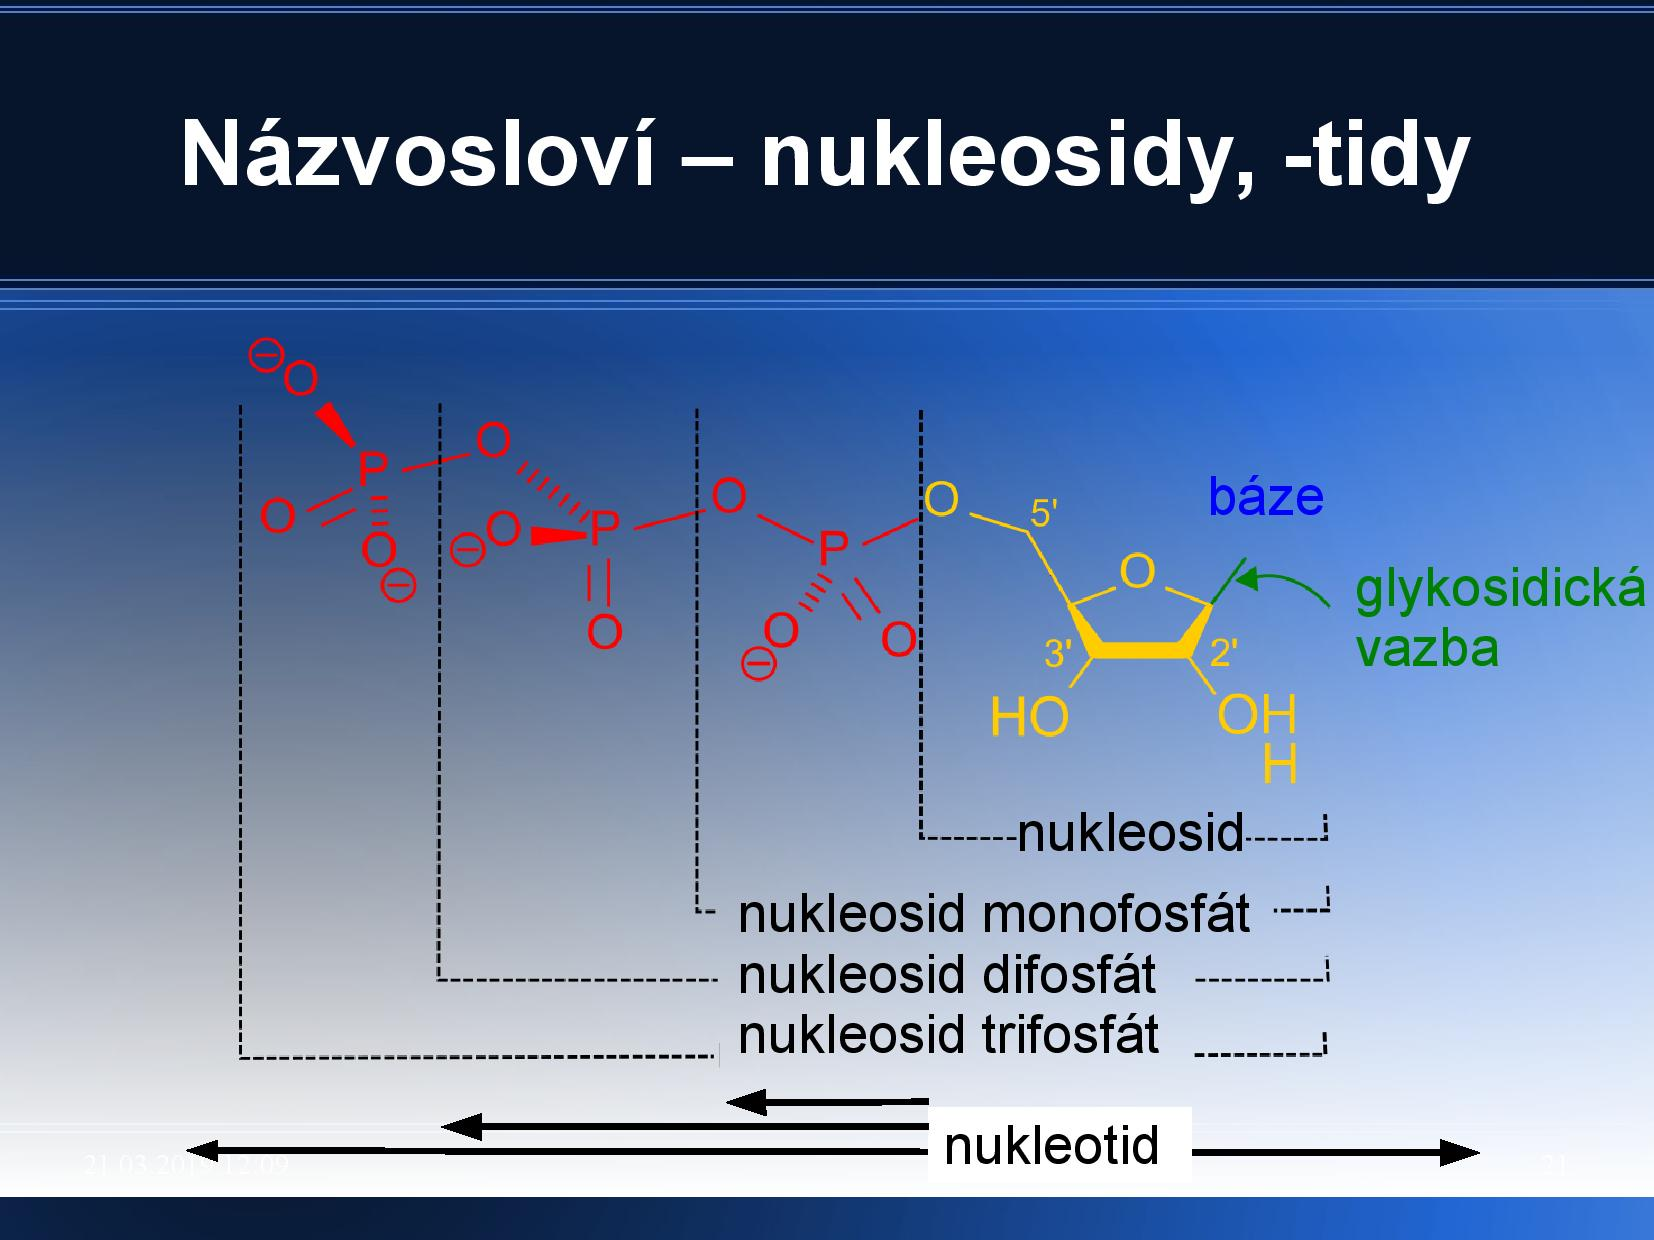
\includegraphics[width=0.85\textwidth]{slides-3/slide-21.jpg}
    \centering
    \label{}
\end{figure}


Názvolsoví nukleotidů a nukleosidů je trochu zmaneté:
\begin{itemize}[nosep]
    \item adenin - adenosin
    \item cytosin - cytidin
    \item guanin - guanosin
    \item thymin - thymidin
    \item uracil - uridin
\end{itemize}



\paragraph{Synklinální a antiklinální forma}
\begin{itemize}[nosep]
    \item rozdělení forem podle toho, na jakou stranu je rotovaná báze
    \item rozlišuje se pouze u purinů
    \item pokud purin míří k cukrfosfátové kostře, jedná se o formu \emph{synklinální}, v opačném případě se jedná o formu \emph{antiklinální}
    \item antiklinální forma je výhodnější, a tedy častější
\begin{itemize}[nosep]
    \item jedinou výjimkou je \hyperref[Konformace Z]{Z forma DNA}
\end{itemize}

\end{itemize}



\mybox{META}{Syn a anti konfigurace \href{http://proteopedia.org/wiki/index.php/Syn_and_anti_nucleosides}{jsou na proteopedii} s pěknými obrázky. A jsou tam i další fajn věci.}


\begin{figure}
    \caption{Prezentace č. 3, slide č. 42}
    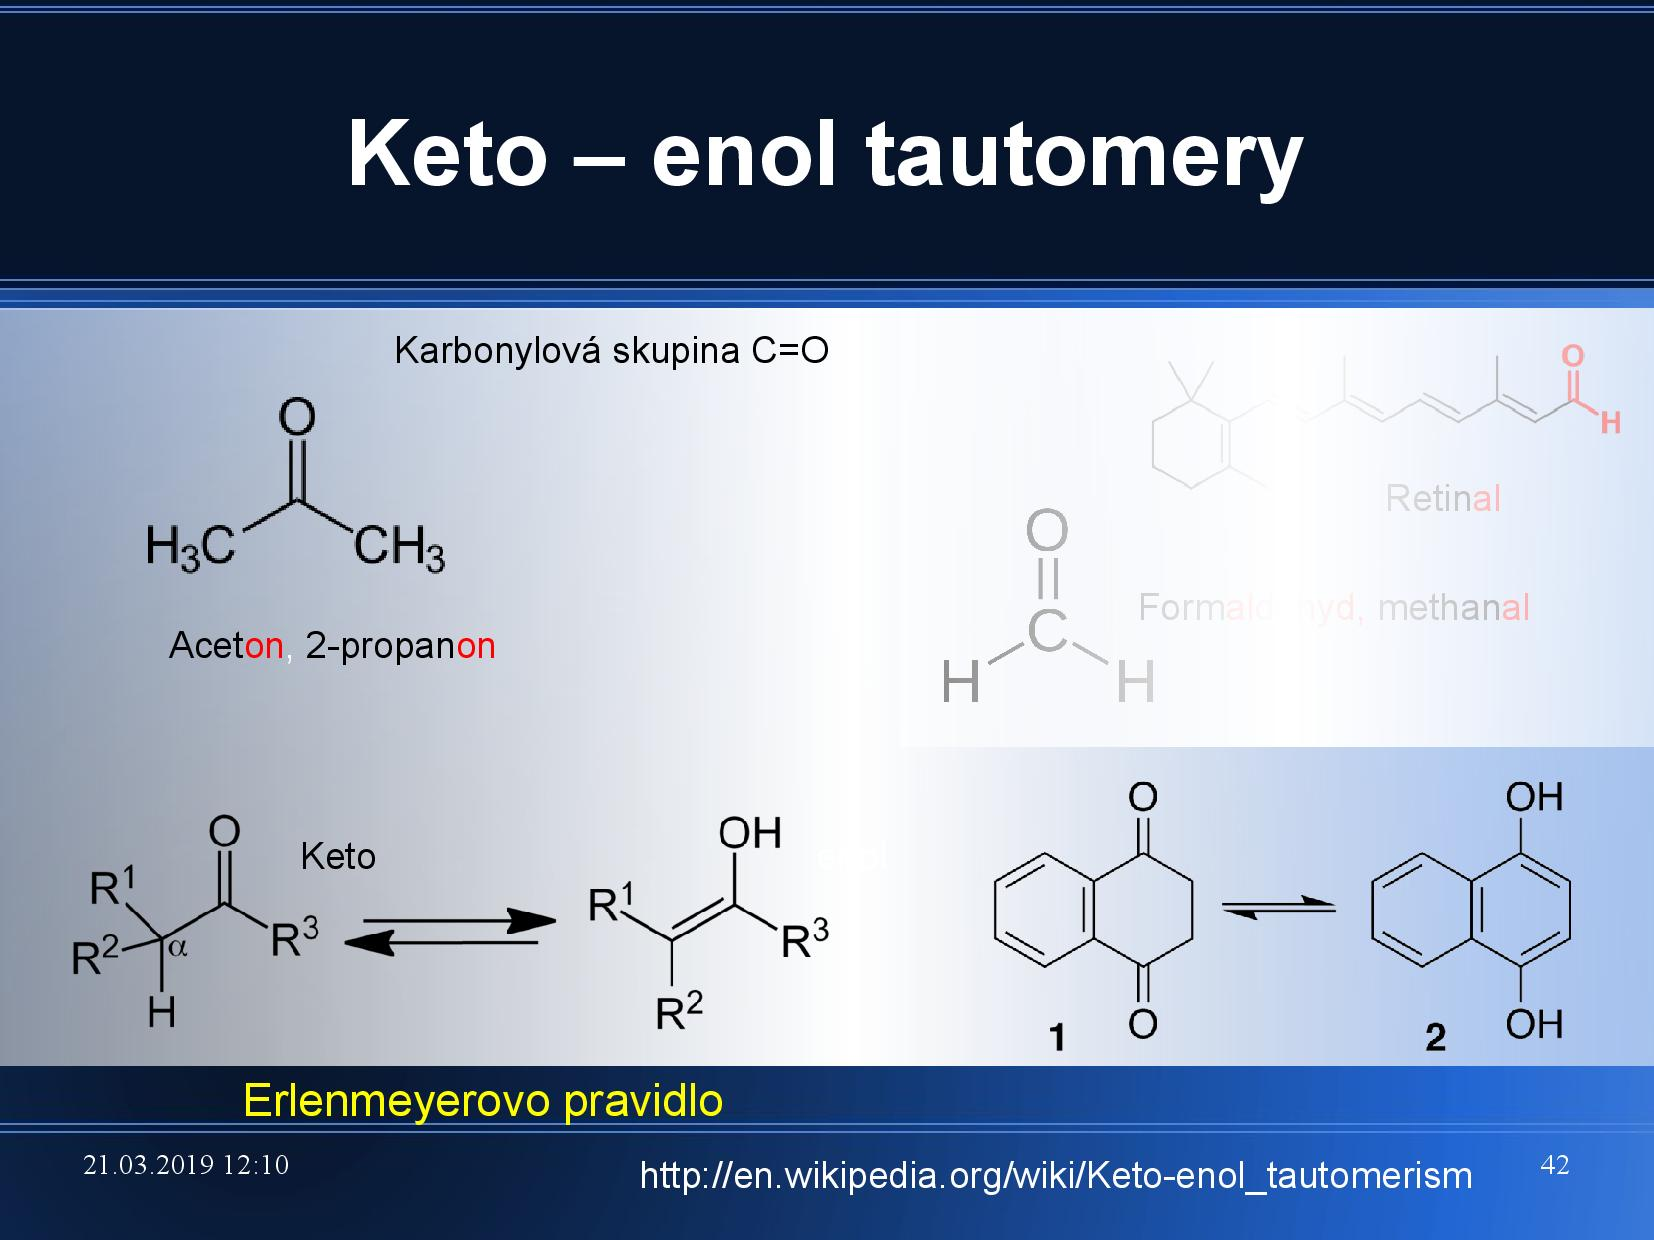
\includegraphics[width=0.85\textwidth]{slides-3/slide-42.jpg}
    \centering
    \label{slides-3-slide-42}
\end{figure}

\paragraph{Keto-enol tautomery}
\begin{itemize}[nosep]
    \item keto skupina
\begin{itemize}[nosep]
    \item uhlík a kyslík vázané dvojnou vazbou
    \item kyslík má vždy volný elektronový pár, funguje jako akceptor vodíkové vazby
\end{itemize}

    \item enol skupina je OH
    \item pokud budeme mít OH skupinu v blízkost idvojné vazby, bude spontánně docházet k přeskupení na keto formu
\begin{itemize}[nosep]
    \item Erlenmeyerovo pravidlo
\end{itemize}

\end{itemize}



\begin{figure}
    \caption{Prezentace č. 3, slide č. 43}
    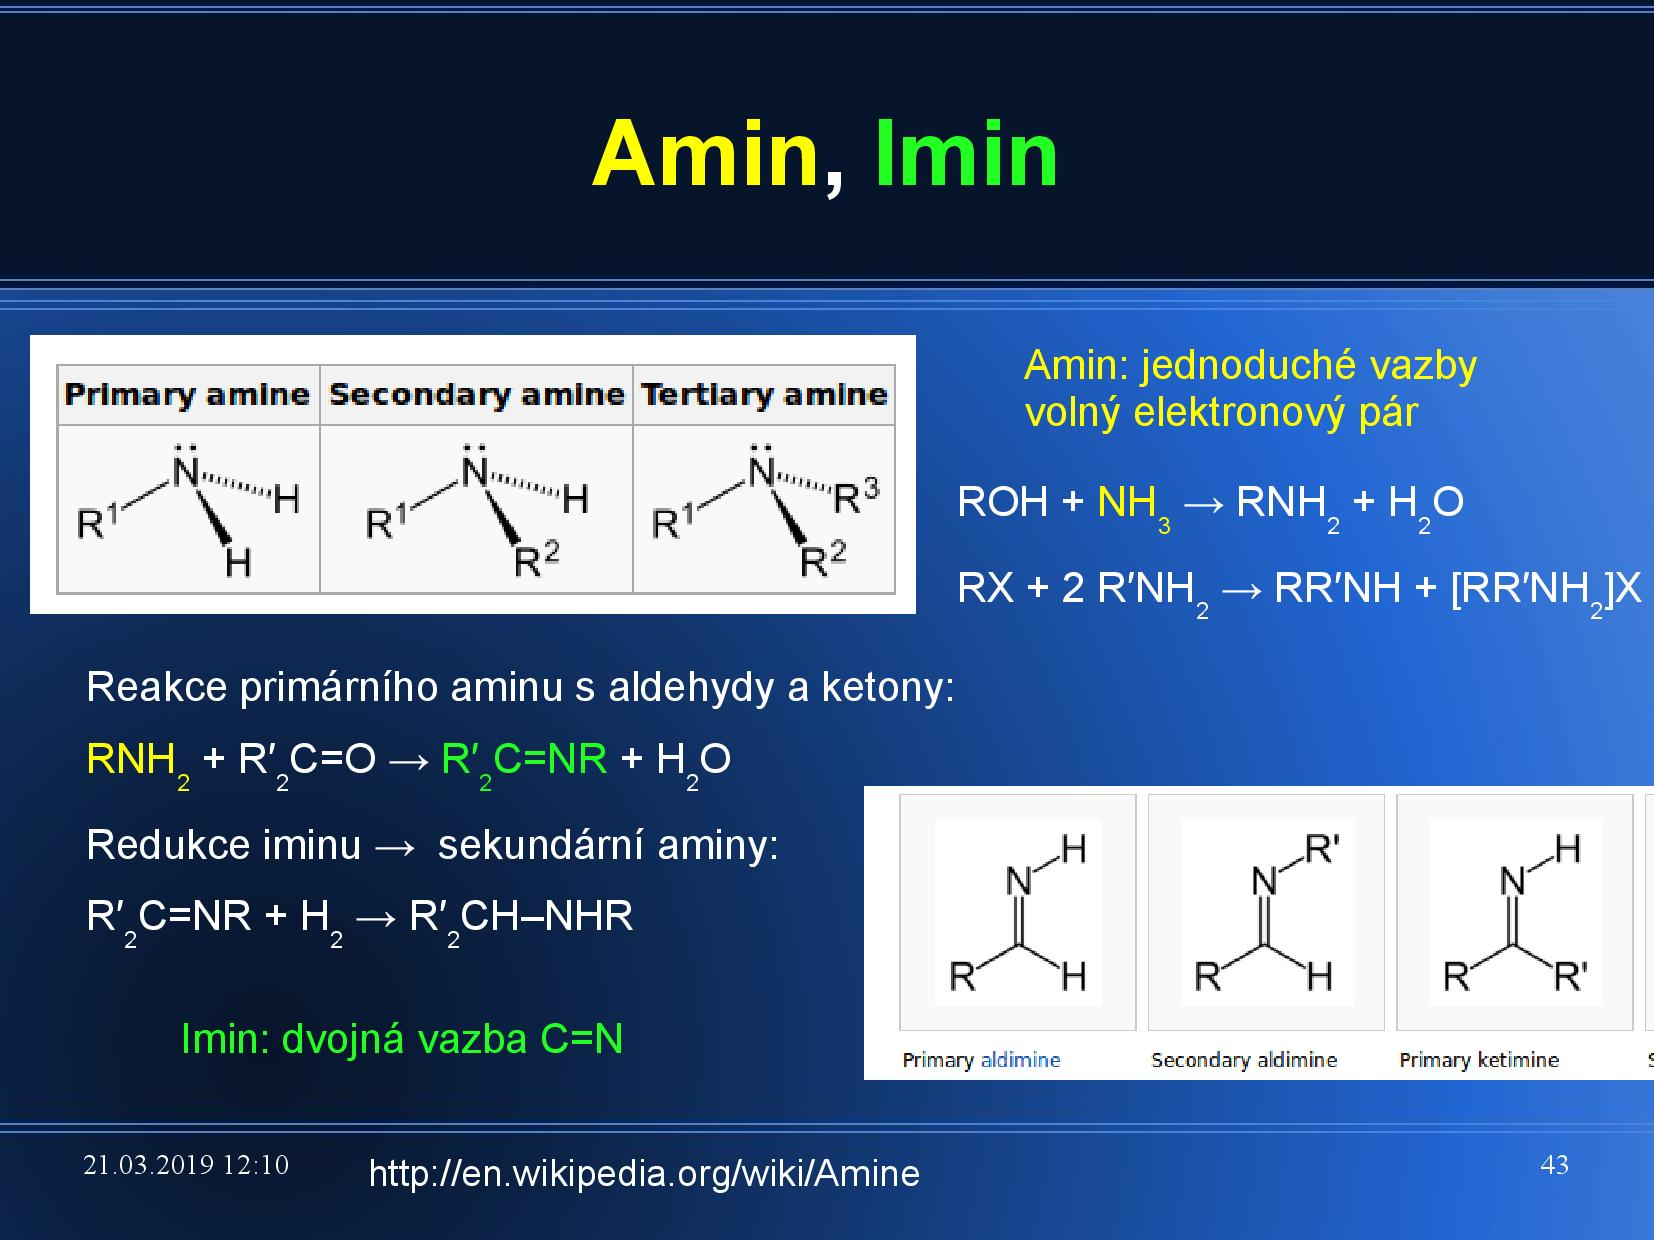
\includegraphics[width=0.85\textwidth]{slides-3/slide-43.jpg}
    \centering
    \label{slides-3-slide-43}
\end{figure}
\begin{figure}
    \caption{Prezentace č. 3, slide č. 44}
    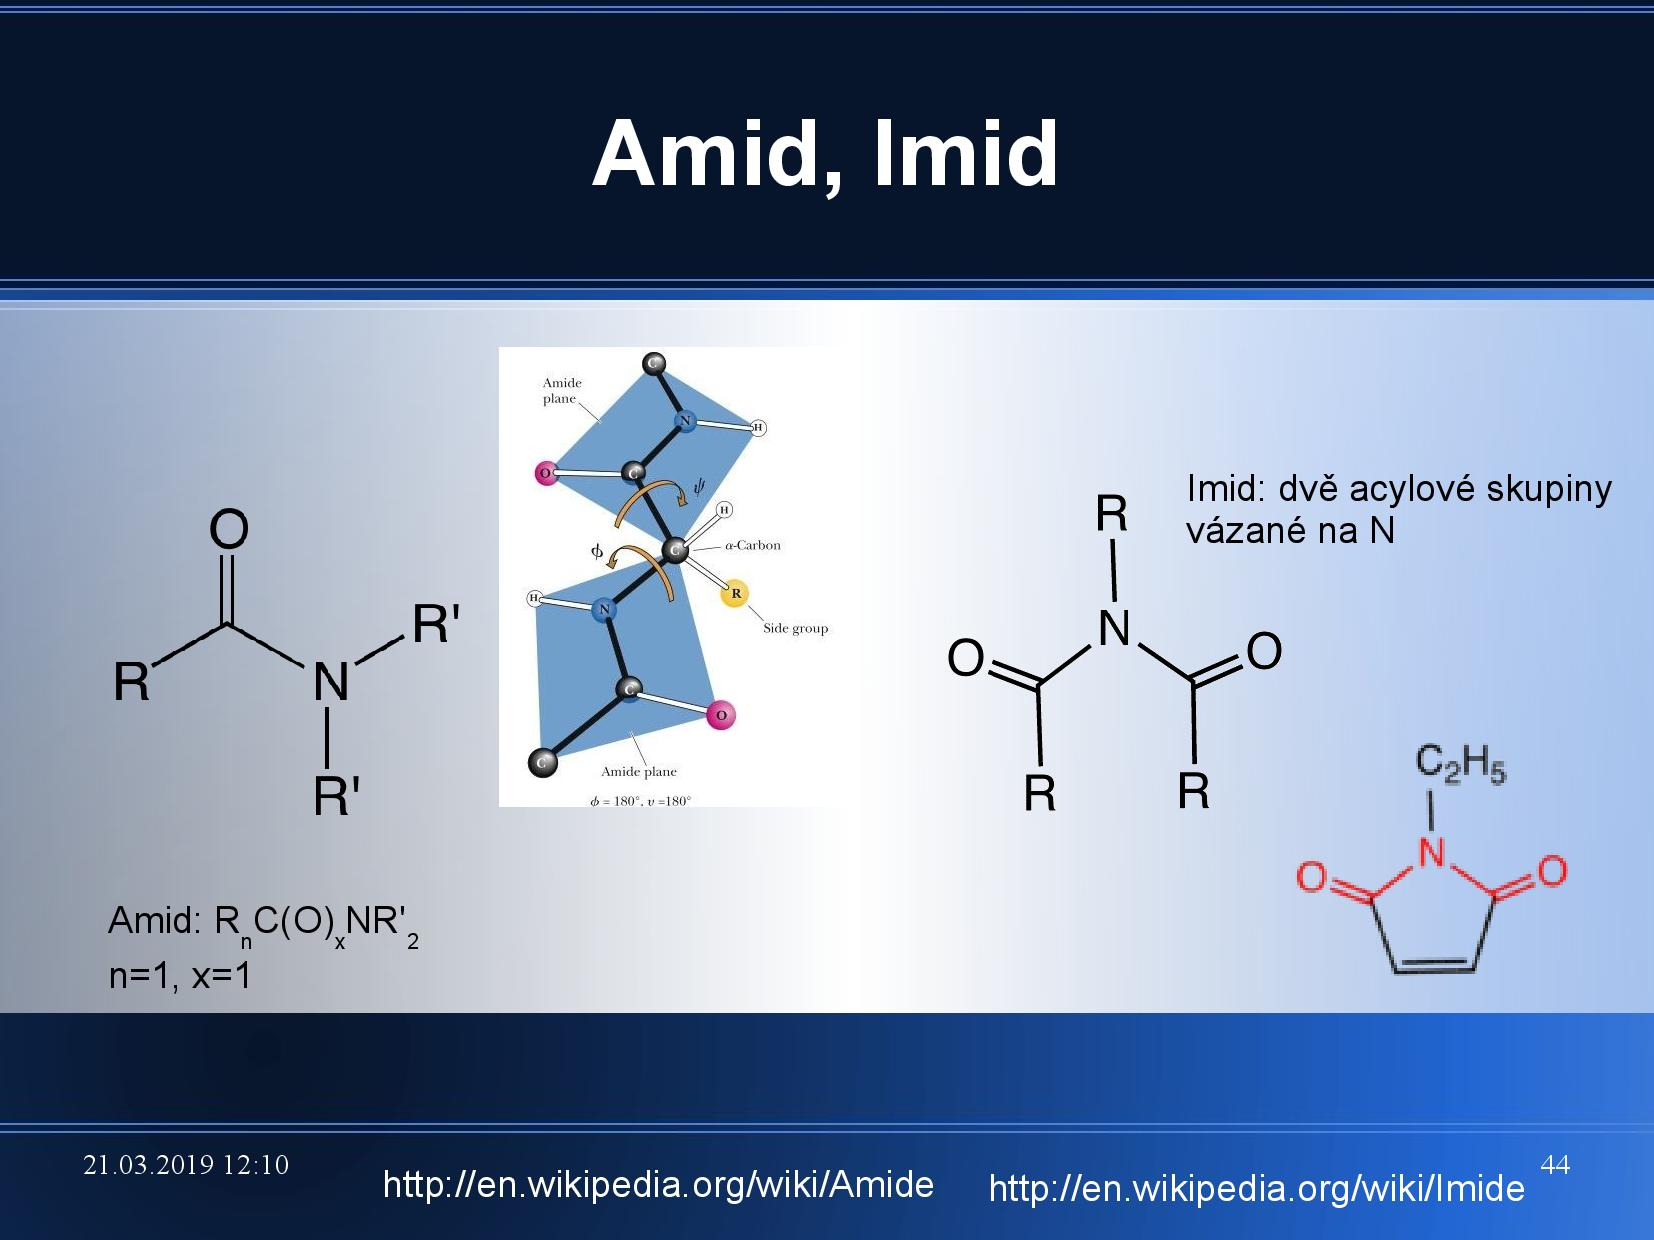
\includegraphics[width=0.85\textwidth]{slides-3/slide-44.jpg}
    \centering
    \label{slides-3-slide-44}
\end{figure}

\paragraph{Amid, imid}
\begin{itemize}[nosep]
    \item primární, sekundární, terciální aminy (viz slide výše)
\begin{itemize}[nosep]
    \item pokud je dusík vázán dvojnou vazbou, jedná se o \emph{imino} skupinu
\end{itemize}

    \item pokud je amin v blízkosti keto skupiny, jedná se o amid
\begin{itemize}[nosep]
    \item podobně existují imidy
\end{itemize}

\end{itemize}



\begin{figure}
    \caption{Tautomery nukleotidů}
    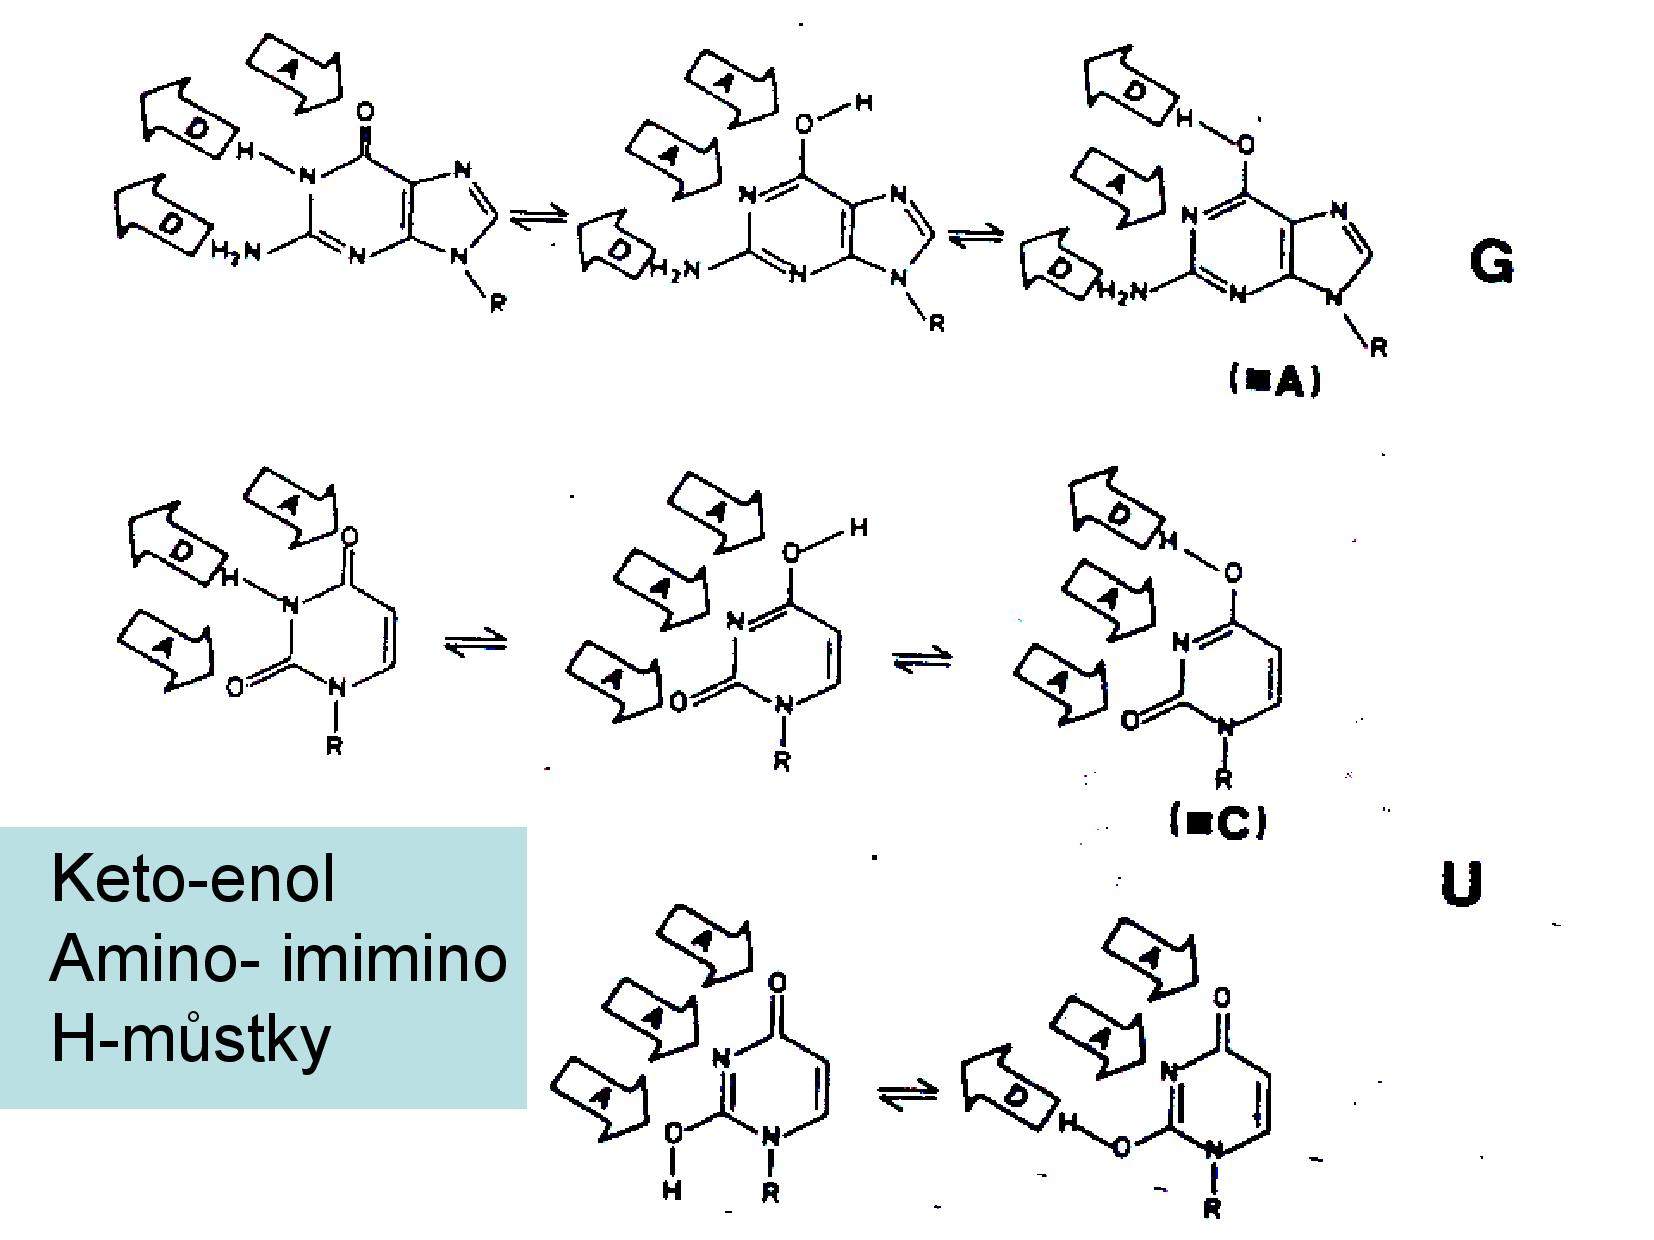
\includegraphics[width=0.85\textwidth]{slides-3/slide-47.jpg}
    \centering
    \label{}
\end{figure}

\begin{figure}
    \caption{Tautomery nukleotidů}
    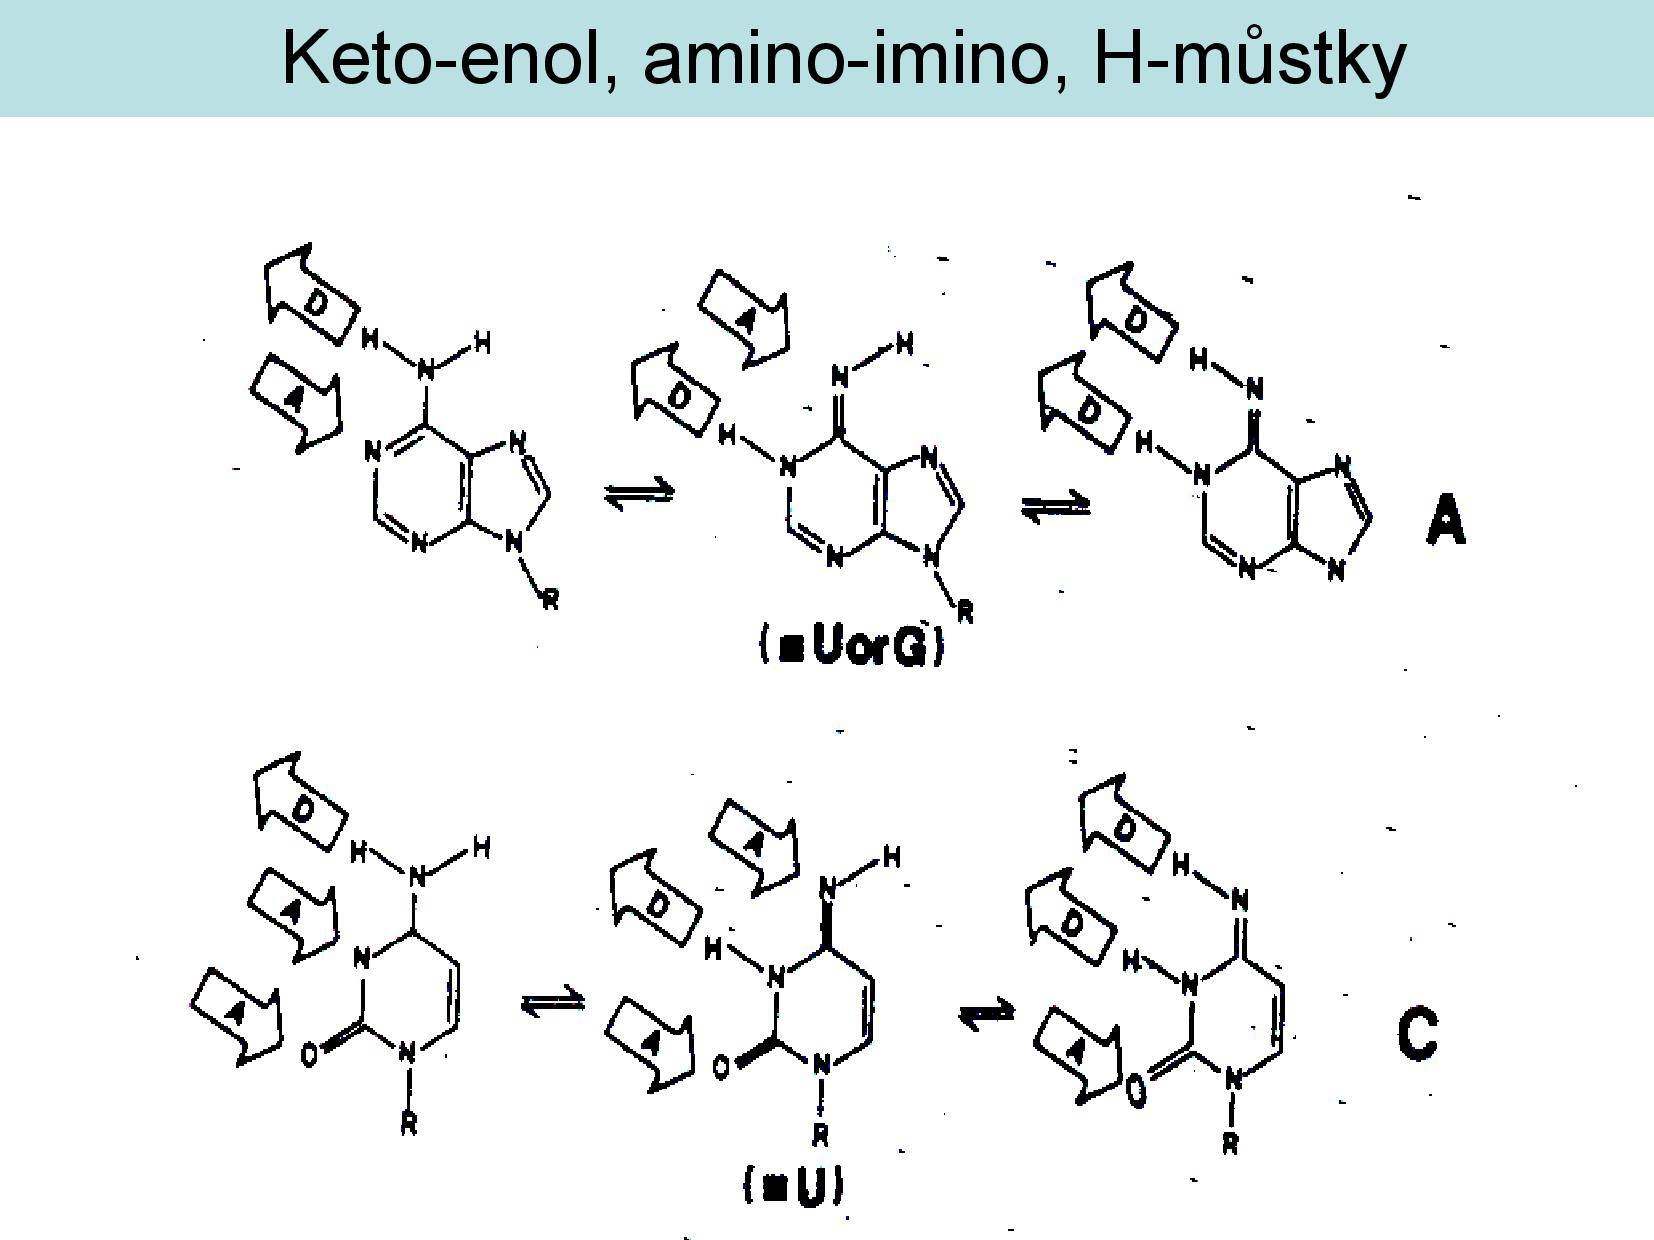
\includegraphics[width=0.85\textwidth]{slides-3/slide-48.jpg}
    \centering
    \label{}
\end{figure}


U všech bazí můžeme pozorovat takzvané \textbf{tautomery}, konkrétně amid+keto nebo imid+enol formy. Přestože jsou amid+keto formy častější, musíme při práci s NA počítat s tím, že semtam mohou mít některé báze velice odlišnou stavbu, totiž imid+enol.

\begin{figure}
    \caption{Prezentace č. 3, slide č. 56}
    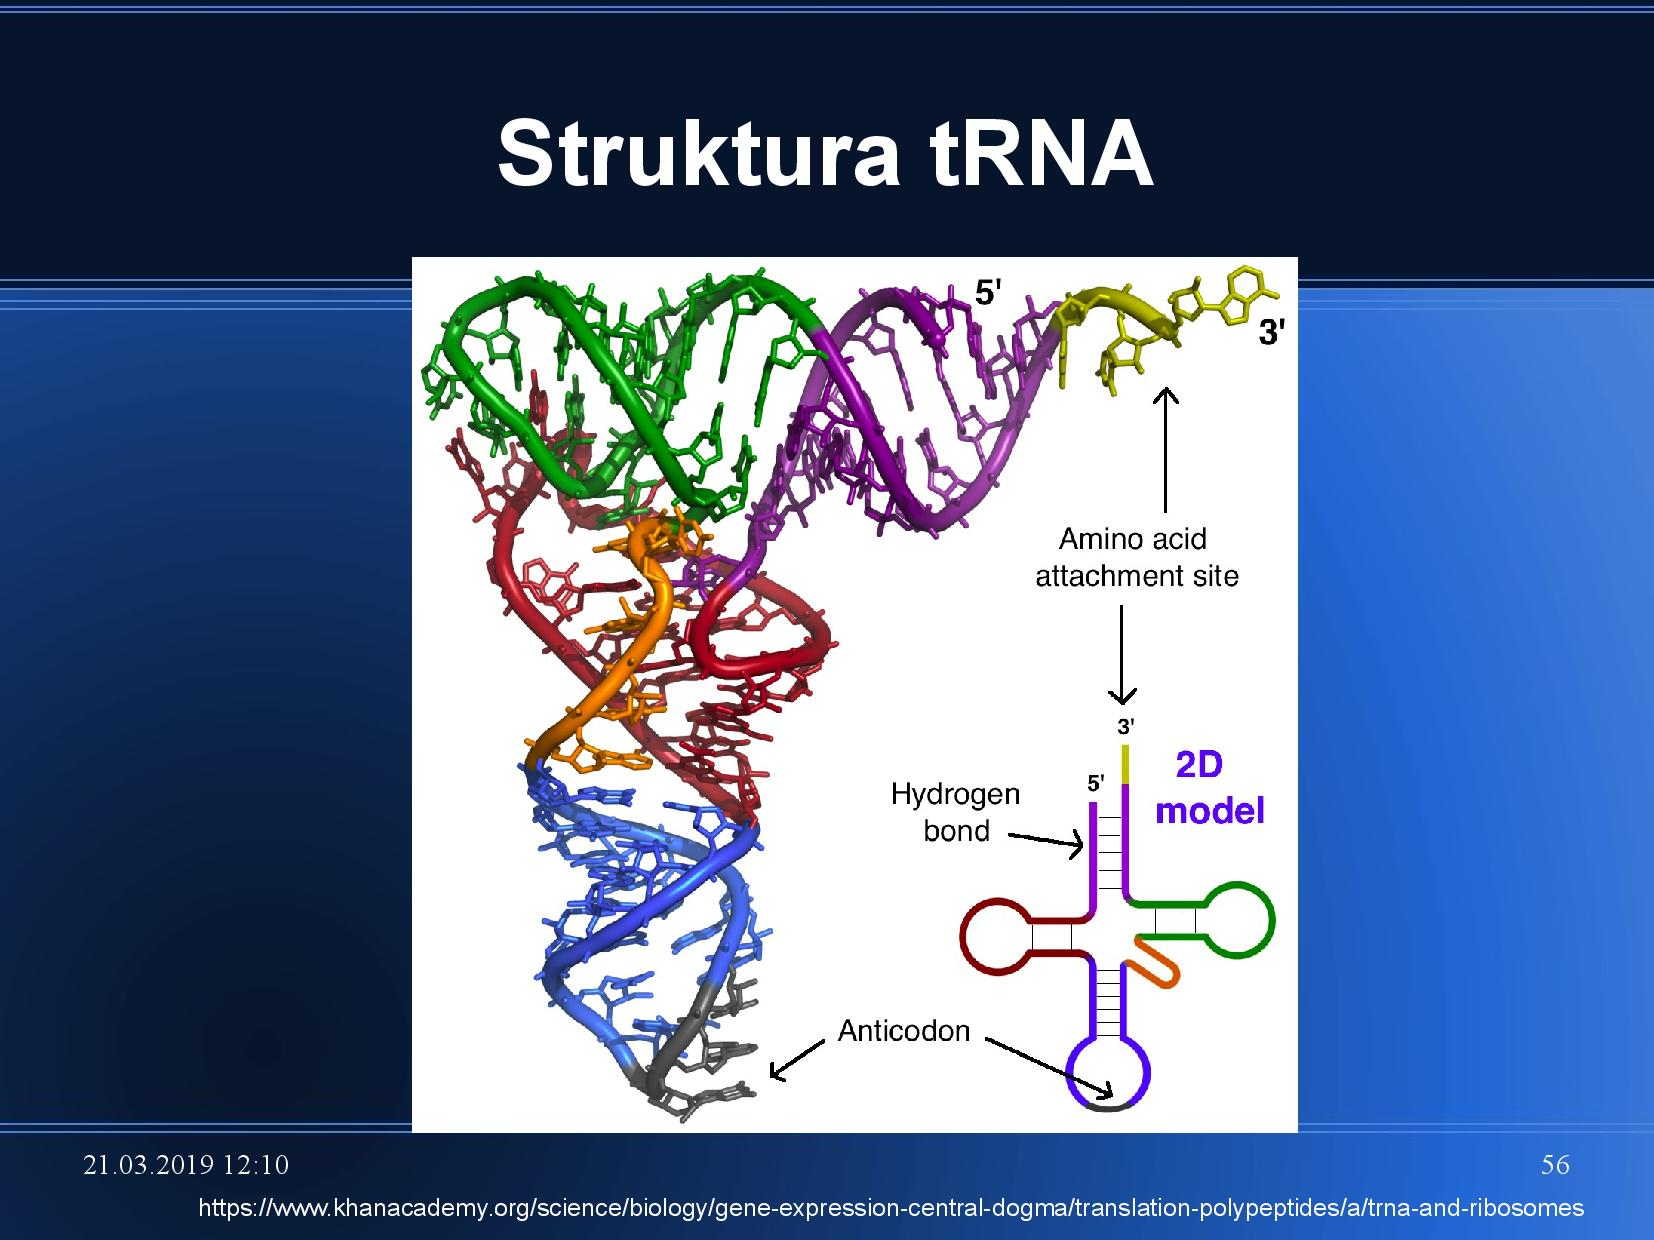
\includegraphics[width=0.85\textwidth]{slides-3/slide-56.jpg}
    \centering
    \label{slides-3-slide-56}
\end{figure}

\paragraph{Struktura tRNA}
\begin{itemize}[nosep]
    \item tři báze dole na smyčce nemají s čím párovat, trčí ven ze smyčky
\begin{itemize}[nosep]
    \item tvoří antikodon, párují s třemi bázemi na mRNA
    \item v jedné z pozic je určitá variabilita, jev \emph{kolísavé párování} (wobbling) => různými triplety je kódovaná stejná AK
\begin{itemize}[nosep]
    \item například ve třetí pozici se může nacházet inosin (hypoxantin + ribóza) \begin{figure}
    \caption{Prezentace č. 3, slide č. 59}
    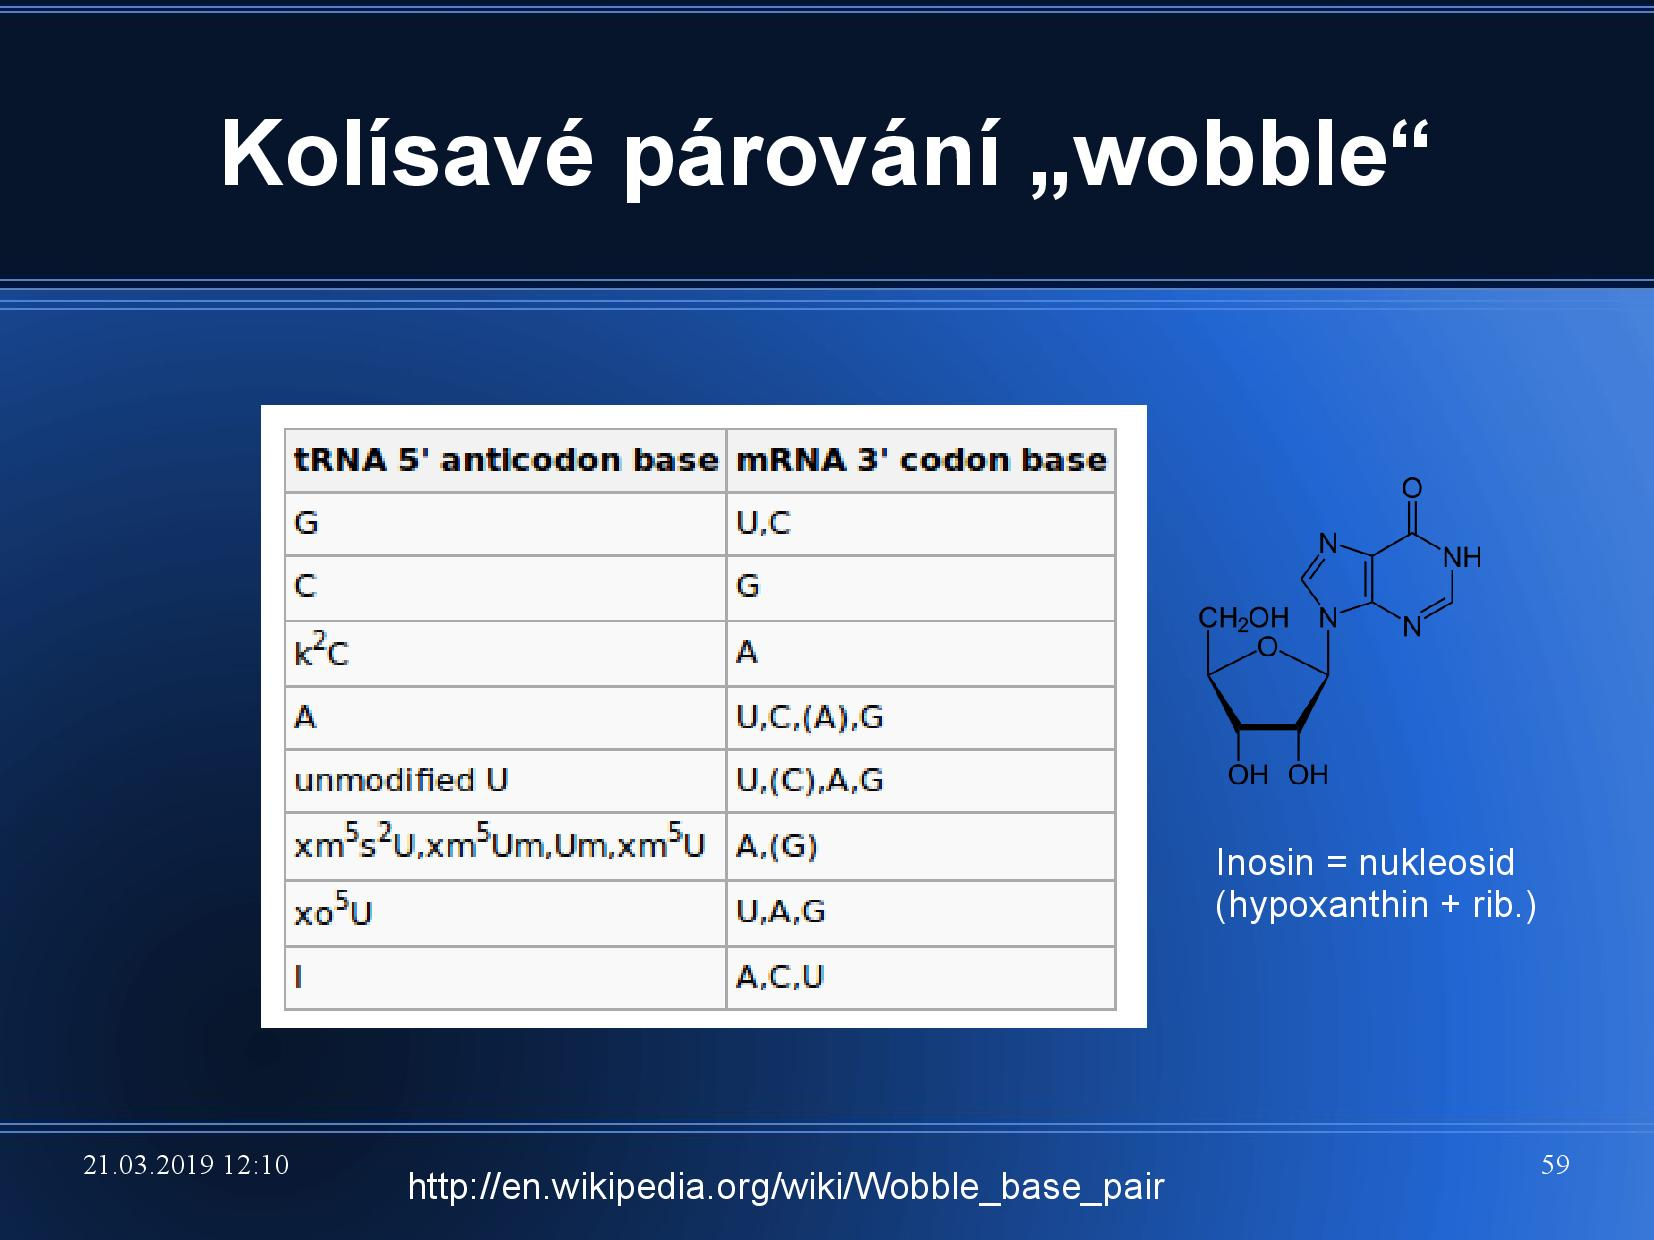
\includegraphics[width=0.85\textwidth]{slides-3/slide-59.jpg}
    \centering
    \label{slides-3-slide-59}
\end{figure}
, který může párovat s C, U i G
    \item tRNA je méně než 64, což je počet, který by byl teoreticky nutný k zakódování všech trojic
\end{itemize}

\end{itemize}

    \item v horní části vázaná AK
\end{itemize}



\subsection{Hoosteenovo párování} \label{Hoosteenovo párování}


Běžné Watson-Crickovo párování je postavené na tom, že spolu párují pouze AT, CG, a všechny puriny jsou v antiklinální podobě. K párování ale může docházet i když jsou puriny v synklinální podobě (zvláště u adeninu, cytosin by musel mít kladný náboj).

\begin{figure}
    \caption{Hoogsteenovo párování}
    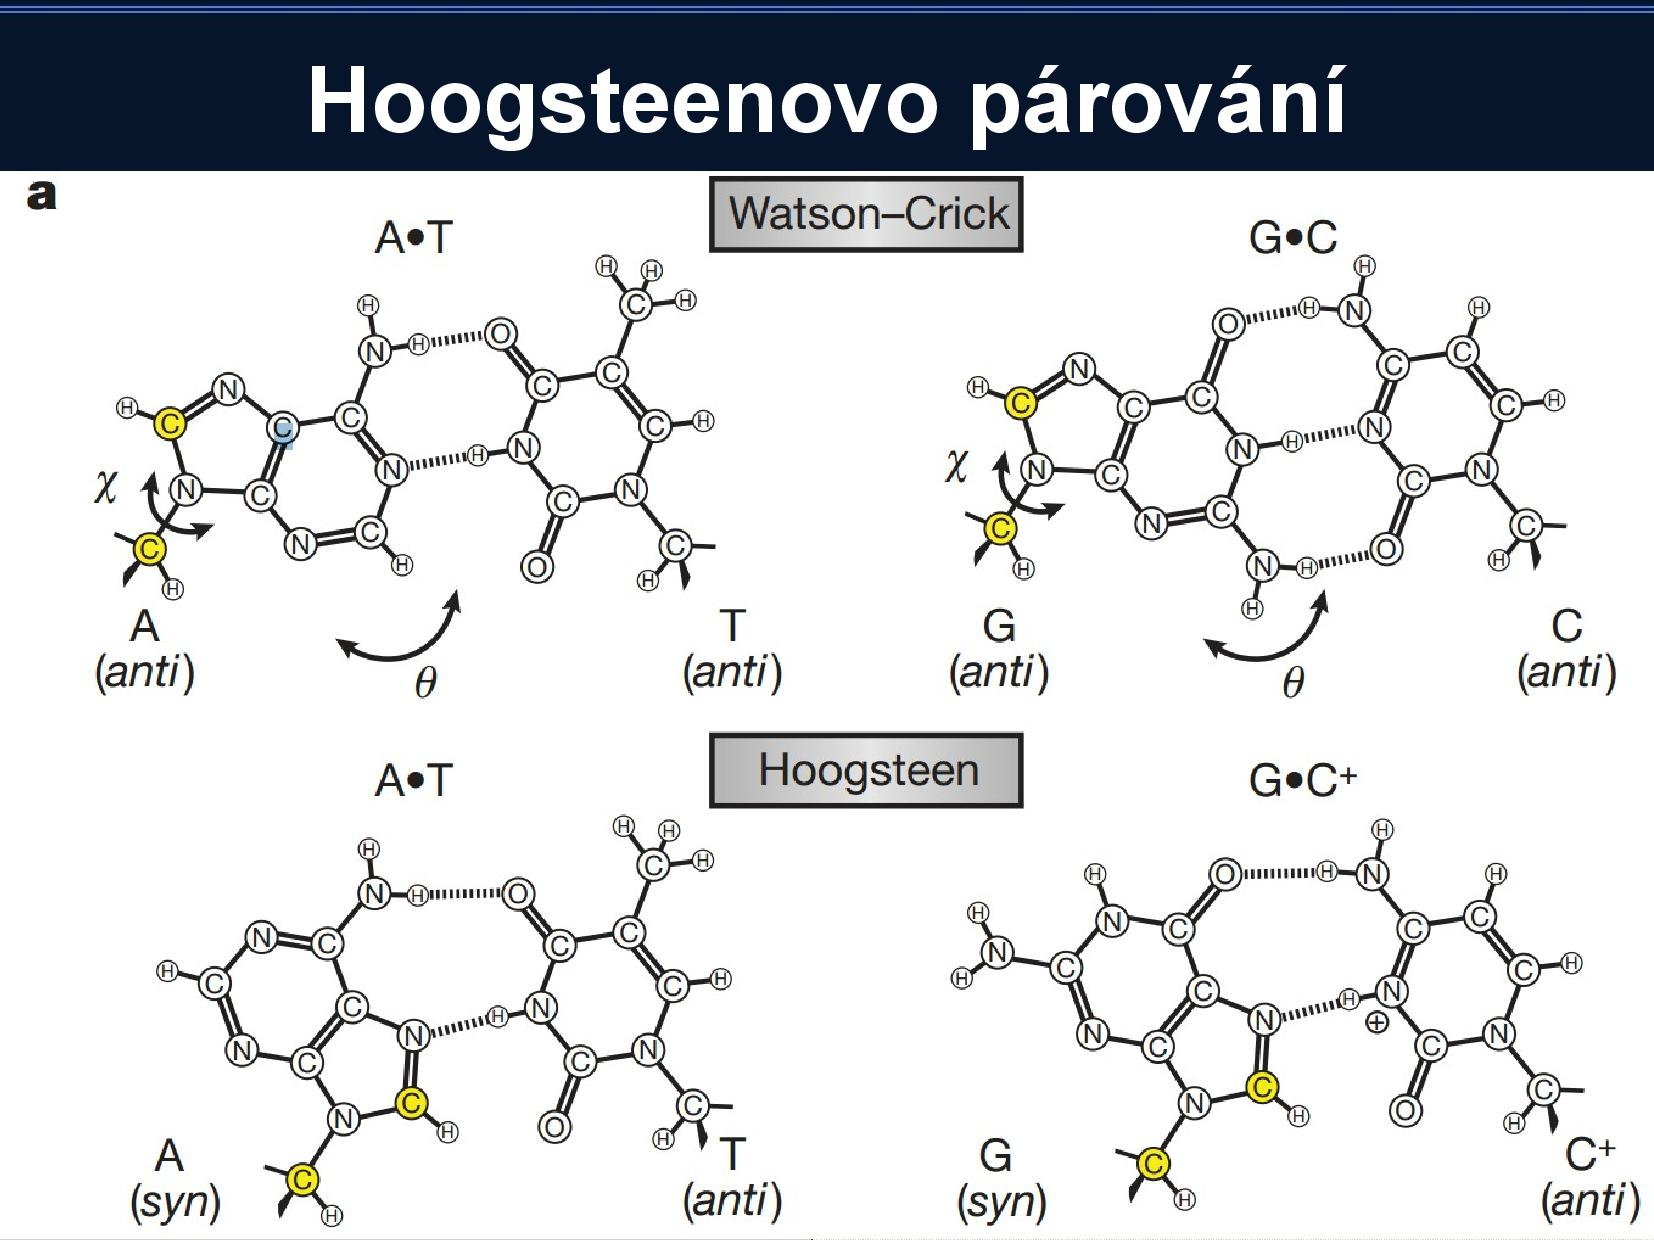
\includegraphics[width=0.85\textwidth]{slides-3/slide-50.jpg}
    \centering
    \label{}
\end{figure}


\begin{figure}
    \caption{Prezentace č. 3, slide č. 51}
    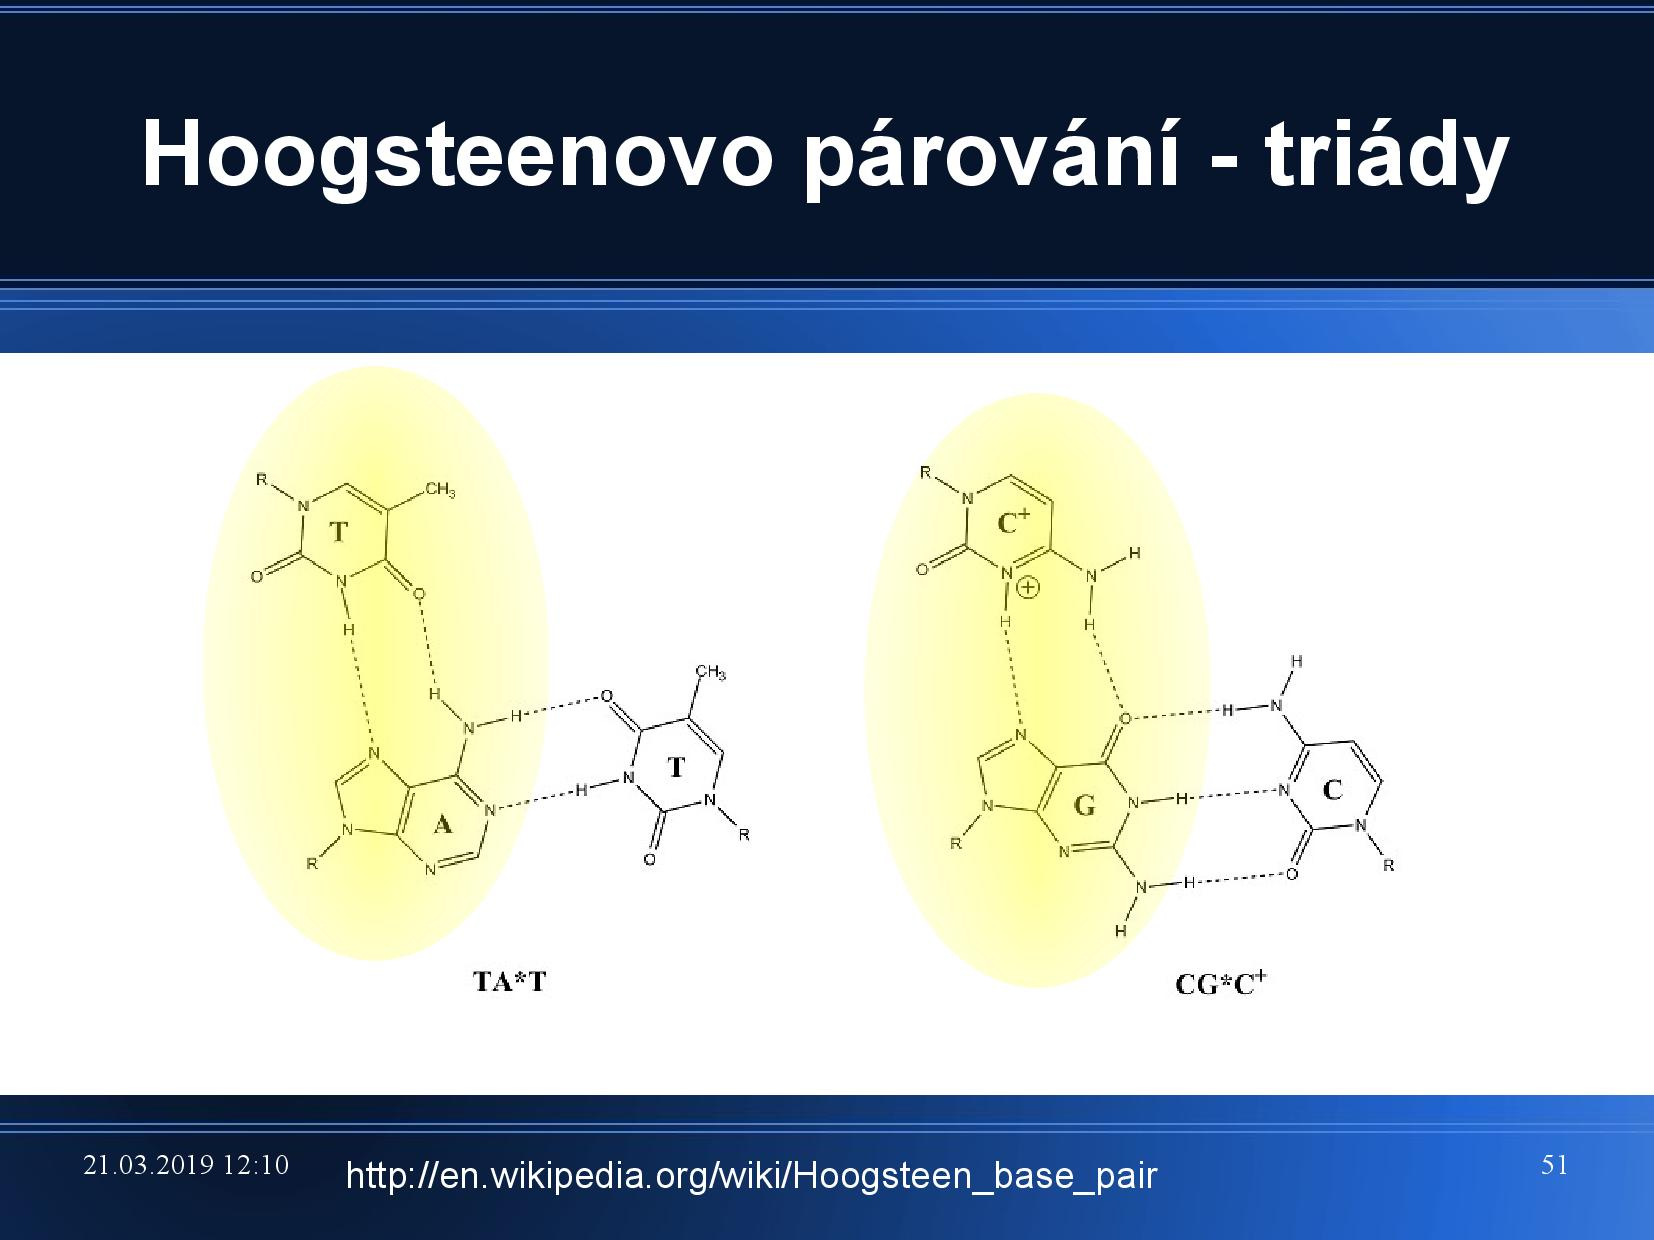
\includegraphics[width=0.85\textwidth]{slides-3/slide-51.jpg}
    \centering
    \label{slides-3-slide-51}
\end{figure}
\begin{figure}
    \caption{Prezentace č. 3, slide č. 52}
    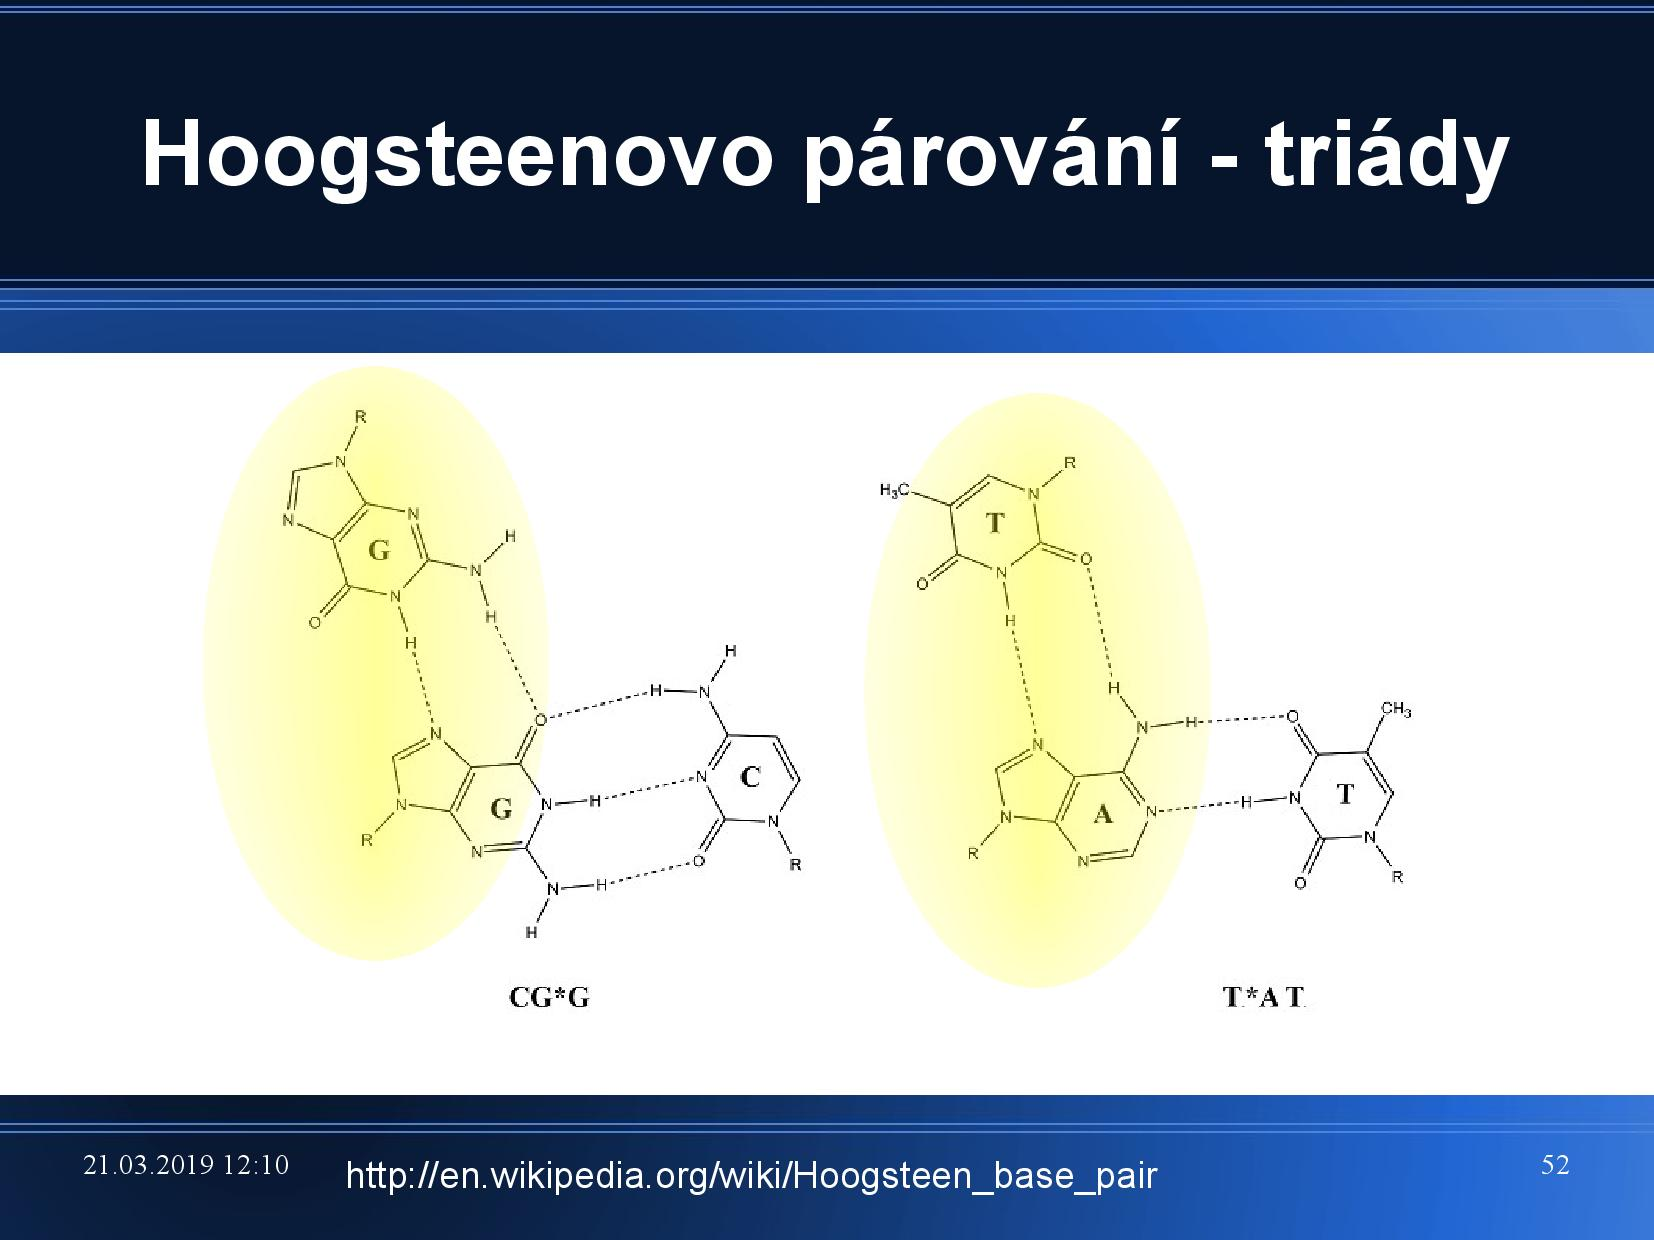
\includegraphics[width=0.85\textwidth]{slides-3/slide-52.jpg}
    \centering
    \label{slides-3-slide-52}
\end{figure}
\begin{figure}
    \caption{Prezentace č. 3, slide č. 53}
    \includegraphics[width=0.85\textwidth]{slides-3/slide-53.jpg}
    \centering
    \label{slides-3-slide-53}
\end{figure}

To znamená, že puriny jsou "na druhé straně" schopny párovat s ještě jednou bazí. Vznikají takzvané \emph{triády}.

\begin{figure}
    \caption{Prezentace č. 3, slide č. 54}
    \includegraphics[width=0.85\textwidth]{slides-3/slide-54.jpg}
    \centering
    \label{slides-3-slide-54}
\end{figure}

\paragraph{G-kvadruplex}
\begin{itemize}[nosep]
    \item čtyři guaniny v jednom patře
\begin{itemize}[nosep]
    \item vlákno se dvakrát ohýbá (viz slide)
\end{itemize}

    \item velice pevná struktura
    \item často v telomerách na koncích chromozomů, aby nebyl degradován endonukleázami
\end{itemize}



Někdy se do běžného DNA helixu vmezeří třetí strand, který se na jedno z vláken naváže H-párováním. Toto třetí vlákno musí mít tzv. polypurinovou část, aby tuto vazbu mohlo vytvořit. Podobně se může mezi vlákna DNA vmezeřit i vlákno RNA.

\section{Reaktivita bazí} \label{Reaktivita bazí}


\begin{figure}
    \caption{Prezentace č. 3, slide č. 63}
    \includegraphics[width=0.85\textwidth]{slides-3/slide-63.jpg}
    \centering
    \label{slides-3-slide-63}
\end{figure}

\begin{itemize}[nosep]
    \item reakce jsou stejné jako u jiných heterocyklických sloučenin
    \item výjimka: pyrimidiny někdy reagují s podobnou molekulou
\begin{itemize}[nosep]
    \item u pyrimidinů je \(\ce{C5=C6}\) podobná izolované dvojné vazbě
    \item naříklad \textbf{thyminový dimer} (viz slide)
    \item při působení UV záření
\end{itemize}

    \item výjimka: alkylace purinů na \(\ce{N7}\) destabilizuje glykosidickou vazbu a vede k depurinaci
\end{itemize}



Většinu bazí můžeme brát jako aromatické molekuly. Součástí interakce bazí jsou tedy i stacking interakce napříč patry.

\chapter{Polymorfismus DNA} \label{Polymorfismus DNA}


\mybox{TODO}{Eeeh, co je to ten polymorfismus?}


\paragraph{Vývoj znalostí o struktuře DNA}
\begin{itemize}[nosep]
    \item první pokusy vycházely z difrakcí rentgenového záření na částečně uspořádaných vláknech dsDNA
\begin{itemize}[nosep]
    \item zjistilo se, že difrakce jsou někdy velice odlišné - tím se pojmenovaly konformace A--Z
\end{itemize}

    \item později se zkoumal rozptyl na krystalech
\begin{itemize}[nosep]
    \item z genomové DNA nešlo udělat krystal -> krystalizovaly se oligonukleotidy, na které byla DNA rozlámaná ultrazvukem
\end{itemize}

    \item na těchto krystalech získáváme informace ještě podrobnější, než na vláknech
\begin{itemize}[nosep]
    \item objev sekvenčního polymorfismu (konkrétní páry bazí si vyžadují odchylky od ideálního strukturního modelu)
\end{itemize}

\end{itemize}



Je ale třeba si uvědomit, že pokud využíváme k detekci anomálií protilátky, můžeme se nám stát, že danou strukturu naší protilátkou stabilizujeme v jedné konkrétní konformaci, i když přirozeně by ji často měnila. Protilátky tak nemusí vždy odrážet realitu.

\mybox{Úhly a reakce}{Řekněme, že pozorujeme interakce dvou molekul v prostoru a vždy měříme úhly, pod kterými jsou spoliu ve styku, z čehož se poté snažíme vyvodit, jestli spolu reagují nějak specificky. Jaké úhly pro nás v tomto případě budou zajímavé?

Jendoduchým pozorováním lze dojít k závěru, že při náhodném umístění a orientaci molekul bude nejběžnější úhel mezi nimi 90\(^{\circ}\), a obecně celé rozložení úhlů ude mít tvar sinusoidy.  Nejvzácnější bude tedy rovnoběžná orientace.

Pokud se tedy naše naměřené úhly budou významně lišit od pravidelné sinusoidy, má cenu se tím dále zabývat.}


\section{Konformační polymorfismus} \label{Konformační polymorfismus}


Jedna molekula DNA bude mít v různých prostředích různou konformaci. Konformací existuje celá řada (A--Z, s různými indexy).

\paragraph{Faktory ovlivňující konformaci}
\begin{itemize}[nosep]
    \item humidita
\begin{itemize}[nosep]
    \item 100\%: B konformace
    \item s ubývajícím množstvím vody -> DNA-A -> DNA-C
\end{itemize}

    \item přítomnost iontů
\begin{itemize}[nosep]
    \item více \(\ce{Mg^{2+}}\) znamená jednodušší metylaci C5' a supercoiling, což způsobuje Z konformaci
\end{itemize}

    \item zastoupení bazí
\begin{itemize}[nosep]
    \item poly-A úseky, poly-AT úseky, atp., mají roznídlné vlastnosti
\end{itemize}

\end{itemize}



\mybox{TODO}{Přepsat tabulku srovnání místo obrázku slidu.}


\begin{figure}
    \caption{Prezentace č. 4, slide č. 20}
    \includegraphics[width=0.85\textwidth]{slides-4/slide-20.jpg}
    \centering
    \label{slides-4-slide-20}
\end{figure}
\begin{figure}
    \caption{Prezentace č. 4, slide č. 22}
    \includegraphics[width=0.85\textwidth]{slides-4/slide-22.jpg}
    \centering
    \label{slides-4-slide-22}
\end{figure}
\begin{figure}
    \caption{Prezentace č. 4, slide č. 24}
    \includegraphics[width=0.85\textwidth]{slides-4/slide-24.jpg}
    \centering
    \label{slides-4-slide-24}
\end{figure}
 Existují tři hlavní rodiny konformací: \textbf{A}, \textbf{B} a \textbf{Z}.


\begin{figure}
    \caption{Prezentace č. 4, slide č. 38}
    \includegraphics[width=0.85\textwidth]{slides-4/slide-38.jpg}
    \centering
    \label{slides-4-slide-38}
\end{figure}


\subsection{Konformace B} \label{Konformace B}


\begin{itemize}[nosep]
    \item nejběžnější
    \item pravotočivá spirálovitá struktura
\begin{itemize}[nosep]
    \item spirálovitá proto, že jednotlivé báze vlastně nechtějí být přesně nad sebou
\end{itemize}

    \item patra jsou vzdálená 330~350pm, působí mezi nimi stacking interakce
    \item fosfáty vzdálené kolem 9Å
    \item C1' uhlíky v rámci patra jsou v každém patře skoro stejně daleko od sebe
    \item ribóza je C2' endo (C2' je na stejnou stranu jako C5')
    \item rozlišení velkého a malého žlábku
\begin{itemize}[nosep]
    \item důležité pro vazby molekul
    \item mnoho proteinů reagujících s DNA funguje jako homodimer reagují s DNA na dvou místech
\begin{itemize}[nosep]
    \item tyto proteiny kromě toho bývají bazické
\end{itemize}

    \item do malého žlábku se váže např. molekula DAPI, která se používá k barvení \begin{figure}
    \caption{Prezentace č. 4, slide č. 9}
    \includegraphics[width=0.85\textwidth]{slides-4/slide-9.jpg}
    \centering
    \label{slides-4-slide-9}
\end{figure}

\end{itemize}

    \item uprostřed helixu není žádné místo
\end{itemize}



\begin{figure}
    \caption{Prezentace č. 4, slide č. 6}
    \includegraphics[width=0.85\textwidth]{slides-4/slide-6.jpg}
    \centering
    \label{slides-4-slide-6}
\end{figure}
\begin{figure}
    \caption{Prezentace č. 4, slide č. 7}
    \includegraphics[width=0.85\textwidth]{slides-4/slide-7.jpg}
    \centering
    \label{slides-4-slide-7}
\end{figure}

\mybox{Malý vs velký žlábek}{Malý a velký žlábek lze rozlišit i na jiných konformacích DNA, kde zpravidla nejdou poznat tak dobře. Způsob jejich určení je naštěstí přesně popsán.
\begin{enumerate}[nosep]
    \item najdeme průsečík osy helixu a nějakého patra DNA
    \item vedeme z tohoto bodu dvě polopřímky, každou do jednoho z C1' na obou bazích
    \item rozdělíme rovinu na dvě části: tam, kde je úhel menší než 180\(^{\circ}\) je malý žlábek, na opačné straně velký žlábek \begin{figure}
    \caption{Prezentace č. 4, slide č. 5}
    \includegraphics[width=0.85\textwidth]{slides-4/slide-5.jpg}
    \centering
    \label{slides-4-slide-5}
\end{figure}

\end{enumerate}

}


\mybox{META}{Byly požadovány znalosti jednotlivých atomů, které se nacházejí ve velkém/malém žlábku.}


\subsection{Konformace A} \label{Konformace A}


\begin{itemize}[nosep]
    \item pravotočivá spirálovitá struktura
    \item ribóza je  C2' exo, C3' endo
    \item uprostřed helixu je dutina, která bývá vyplněna vodou
\begin{itemize}[nosep]
    \item někdy se stane, že dvě báze spolu interagují prostřednictvím molekuly vody
\end{itemize}

\end{itemize}



Podobnou konformaci zaujímá i heterokomlex DNA+RNA, protože OH skupina cukru z RNA musí čnít ven z helixu, tedy C2' musí být exo.

\subsection{Konformace Z} \label{Konformace Z}


\begin{itemize}[nosep]
    \item levotočivá spirálovitá struktura
    \item kostra uspořádaná zig-zag
\begin{itemize}[nosep]
    \item v sekvenci se střídají puriny a pyrimidiny
\begin{itemize}[nosep]
    \item puriny jsou synklinální, jejich riboza je tedy přetočená a kostra vypadá zig-zag
\end{itemize}

\end{itemize}

    \item patra jsou si strukturou podobná ob jedno (v B jsou si podobná všechna), repetitivní je dvojice párů bazí nad sebou
    \item některé modifikace bazí (například methylace na C5') Z konformaci stabilizují (methyl se dobře schová mezi dvě patra)
    \item převládaají báze G a C
\end{itemize}



\section{Sekvenční polymorfismus} \label{Sekvenční polymorfismus}


\begin{figure}
    \caption{Prezentace č. 4, slide č. 43}
    \includegraphics[width=0.85\textwidth]{slides-4/slide-43.jpg}
    \centering
    \label{slides-4-slide-43}
\end{figure}
\begin{figure}
    \caption{Prezentace č. 4, slide č. 46}
    \includegraphics[width=0.85\textwidth]{slides-4/slide-46.jpg}
    \centering
    \label{slides-4-slide-46}
\end{figure}
\begin{figure}
    \caption{Prezentace č. 4, slide č. 47}
    \includegraphics[width=0.85\textwidth]{slides-4/slide-47.jpg}
    \centering
    \label{slides-4-slide-47}
\end{figure}
\begin{figure}
    \caption{Prezentace č. 4, slide č. 49}
    \includegraphics[width=0.85\textwidth]{slides-4/slide-49.jpg}
    \centering
    \label{slides-4-slide-49}
\end{figure}
 Báze v rámci patra nejsou v rovině, ale zaujímají tvar asymetrické vrtule. Stejně tak jednotlivá patra spolu nejsou rovnoběžná, ale různě nepravidelně natočená, protože si navzájem přkážejí.

\begin{figure}
    \caption{Prezentace č. 4, slide č. 52}
    \includegraphics[width=0.85\textwidth]{slides-4/slide-52.jpg}
    \centering
    \label{slides-4-slide-52}
\end{figure}
\begin{figure}
    \caption{Prezentace č. 4, slide č. 54}
    \includegraphics[width=0.85\textwidth]{slides-4/slide-54.jpg}
    \centering
    \label{slides-4-slide-54}
\end{figure}
 Natočení a posun bazí je různý u různých konformací DNA, a závisí také na místním nukleotidovém složení. Zajímavě se například chovají poly-AT regiony. \begin{figure}
    \caption{Prezentace č. 5, slide č. 10}
    \includegraphics[width=0.85\textwidth]{slides-5/slide-10.jpg}
    \centering
    \label{slides-5-slide-10}
\end{figure}


\begin{figure}
    \caption{Prezentace č. 4, slide č. 16}
    \includegraphics[width=0.85\textwidth]{slides-4/slide-16.jpg}
    \centering
    \label{slides-4-slide-16}
\end{figure}
\begin{figure}
    \caption{Prezentace č. 4, slide č. 17}
    \includegraphics[width=0.85\textwidth]{slides-4/slide-17.jpg}
    \centering
    \label{slides-4-slide-17}
\end{figure}
 Se sekvencí se nemění pouze posun bazí, ale i možné torzní úhly. Na slidu jsou znázorněny torzní úhly dvou polyadenylylových úseků s různými majoritními nukleotidy.

\section{Dynamický polymorfismus} \label{Dynamický polymorfismus}


\begin{figure}
    \caption{Prezentace č. 4, slide č. 56}
    \includegraphics[width=0.85\textwidth]{slides-4/slide-56.jpg}
    \centering
    \label{slides-4-slide-56}
\end{figure}

DNA je neustále v pohybu. Jak moc a jakým způsobem záleží především na konkrétní sekvenci.

\begin{itemize}[nosep]
    \item nedá se sledovat na krystalech, musíme použít NMR nebo například fluorescenci
    \item jedná se vlastně o časově a prostorově lokální denaturaci
    \item pokud například DNA-B přechází v DNA-Z, jedna báze se může vyklopit z řetězce (flipování)
\begin{itemize}[nosep]
    \item často proto, že reaguje s nějakým enzymem
\end{itemize}

\end{itemize}



\paragraph{Denaturace}
\begin{itemize}[nosep]
    \item rozpad helikální struktury DNA, většinou způsobený teplem
    \item DNA se rozplétá od konců, nebo v sousedství utajených přerušení
    \item poly-AT úseky tají první, protože AT jsou spojeny jen dvěma vodíkovými můstky
    \item pokud k renaturaci dojde příliš rychle (např. prudkým ochlazením), ne všechny báze musí nutně skončit se svou komplentární dvojicí
\end{itemize}



\section{Ohyby a zalomení} \label{Ohyby a zalomení}


K ohybům dochází v DNA hlavně na základě sekvenčního polymorfismu a na hranici dvou konformací. Naopak k zalomení především v důsledku mechanického namáhání nebo při vazbě na zakřivený povrch.

\begin{figure}
    \caption{Prezentace č. 4, slide č. 66}
    \includegraphics[width=0.85\textwidth]{slides-4/slide-66.jpg}
    \centering
    \label{slides-4-slide-66}
\end{figure}

\paragraph{Ohyb vlákna}
\begin{itemize}[nosep]
    \item způsoben AT bohatými oblastmi
    \item A a T spolu mohou reagovat napříč patry, čímž se DNA ohne
    \item DNA se částečně rozplete a sekvence jsou dobře dostupné
\begin{itemize}[nosep]
    \item => často v promotorových nebo regulačních oblastech
\end{itemize}

\end{itemize}



\section{Další konformační anomálie} \label{Další konformační anomálie}


\begin{figure}
    \caption{Prezentace č. 4, slide č. 69}
    \includegraphics[width=0.85\textwidth]{slides-4/slide-69.jpg}
    \centering
    \label{slides-4-slide-69}
\end{figure}

\begin{itemize}[nosep]
    \item lokální úseky Z-DNA, H-DNA, A-DNA, 4s DNA (uvnitř molekuly B-DNA)
    \item při výskytu palindromu, kde je jeden úsek DNA komplementární s nadcházejícícm úsekem na stejném vlákně, někdy na DNA vznikne kříž
    \item kromě kříže vlásenky, bubliny
    \item utajená přerušení: jedno vlákno je na kostře přerušené
\begin{itemize}[nosep]
    \item nejsou problém, vlákna u sebe drží velkou silou
    \item začíná u nich denaturace
\end{itemize}

    \item gapy: místa, kde chybí nějaká báze
    \item zlom s adhezivními (lepivými) přesahujícími konci: vlákno se lepí na vlákno podobného tvaru, nezáleží ale na jejich původu; adhezivní konce umožňují vytvářet genetické změny v DNA, můžeme je míchat
\end{itemize}



\paragraph{Způsoby studia strukturních anomálií}
\begin{itemize}[nosep]
    \item můžeme využít hypersenzitivity anomálií
\begin{itemize}[nosep]
    \item nukleázy (S1, mikrokokální)
    \item chemické modifikace (glyoxal, chloracetaldehyd)
\end{itemize}

    \item můžeme detekovat chemicky značené anomlie
\begin{itemize}[nosep]
    \item  elektronová mikroskopie
    \item denaturační křivky
    \item elektroforéza
    \item sekvenování
    \item vazba protilátek
\end{itemize}

\end{itemize}



\section{Vsuvka: konformace RNA} \label{Vsuvka: konformace RNA}


\begin{figure}
    \caption{Prezentace č. 5, slide č. 2}
    \includegraphics[width=0.85\textwidth]{slides-5/slide-2.jpg}
    \centering
    \label{slides-5-slide-2}
\end{figure}

\paragraph{RNA vlásenka}
\begin{itemize}[nosep]
    \item často se objevují nezvyklá párování
\begin{itemize}[nosep]
    \item U + fosfátová skupina
    \item G+U, U+U a podobně
\begin{itemize}[nosep]
    \item někdy stabilizováno přes molekulu vody
\end{itemize}

    \item G někdy tvoří vodíkový můstek s ribozou
\end{itemize}

    \item uracil a cytosin na špičce s ničím nepárují
\begin{itemize}[nosep]
    \item cytosin stacking interaguje s párem pod sebou
    \item uracil ční do prostoru (nejspíš málo konzervovaná pozice)
\end{itemize}

    \item na špičce vlásenky často UUCG a podobné
\end{itemize}



\paragraph{Bazická hydrolýza RNA}
\begin{enumerate}[nosep]
    \item ve vysokém pH (silně zásadité) dojde k deprotonizaci \(\ce{OH}\) skupiny na ribóze
    \item kyslík z ribózy může nukleofilně reagovat s fosfátem z RNA kostry
    \item fosfát je en čtyřvazebný a tak jednu ze stávajících vazeb přeruší
    \item RNA se rozpadne
    \item fosfát posléze zůstane jen na C2' nebo C3'
\end{enumerate}



Podobně fungují i enzymy štěpící RNA, je proto relativně složité je zastavit (např. u DNA stačí jen odebrat z roztoku kovy, které enzymy potřebují k rozložení DNA).

\begin{figure}
    \caption{Prezentace č. 4, slide č. 77}
    \includegraphics[width=0.85\textwidth]{slides-4/slide-77.jpg}
    \centering
    \label{slides-4-slide-77}
\end{figure}
 V ribozomálním RNA jsou někdy celé sítě různých interakcí mezi nukleotidy.

\begin{figure}
    \caption{Prezentace č. 5, slide č. 4}
    \includegraphics[width=0.85\textwidth]{slides-5/slide-4.jpg}
    \centering
    \label{slides-5-slide-4}
\end{figure}
 V RNA je možných mnoho různých druhů párování.

\section{Topologie DNA} \label{Topologie DNA}


DNA má strukturu dihelixu, viz výše. Topologie DNA se zabývá tím, jaký tvar tento dihelix zaujme v prostoru.

\begin{description}
\item[supercoil]\hfill \\
Supercoil (neboli \emph{nadobrátky}) je termín, který popisuje přetočení nebo podtočení dihelixu DNA, které je vyústěním nějakého vnitřního tlaku, který na vlákna působí. Supercoil vzniká například v bakteriálním plazmidu. \begin{figure}
    \caption{Prezentace č. 5, slide č. 14}
    \includegraphics[width=0.85\textwidth]{slides-5/slide-14.jpg}
    \centering
    \label{slides-5-slide-14}
\end{figure}
 DNA v přírodě se většinou vyskytuje právě v této formě.

Supercoilu se říká také \emph{superhelix}, nadobrátkám někdy terciární vinutí (běžné Watson-Crickovské je sekundární).
\begin{figure}
    \caption{Znázornění nadobrátek}
    \includegraphics[width=0.85\textwidth]{supercoil.jpg}
    \centering
    \label{}
\end{figure}



\item[relaxovaná pozice]\hfill \\
DNA je v relaxované pozici, když nemá žádné nadobrátky. Relaxovaná cyklická DNA (například plazmid) se označuje jako CO forma ()


\item[twisting number (T)]\hfill \\
Udává počet překřížení dvou vláken DNA, která jsou spolu v dihelixu. DNA je před spočítáním \(T\) nejprve vyrovnat do plochy. Znaménko udává, jestli je helix pravotočivý (\(+\)) nebo levotočivý (\(-\)).

V běžných podmínkách u lineárních B-DNA bývá \(T = 10\) na každých 106bp, protože B-DNA má jednu otočku na přibližně 10.6 párů bazí. \begin{figure}
    \caption{Znázornění nadobrátek}
    \includegraphics[width=0.85\textwidth]{twist_and_writhe.png}
    \centering
    \label{}
\end{figure}



\item[writhe number (W)]\hfill \\
Udává počet nadobrátek, v přírodě (u bakteriálních plazmidů) bývá \(W = 1\) na 200bp. Nadobrátky mohou vyústit ve dvojí typ topologie: DNA zaujme buďto toroidální tvar, nebo plektonemní tvar. Plektonemnímu tvaru se někdy říká \emph{dvojitá nadšroubovice}.

\mybox{Poznámka}{Toroid je nějaký tvar, který rotuje kolem nějaké osy. Plektonem je v překladu "zkroucené vlákno" a vypadá spíše jako řetěz. \begin{figure}
    \caption{Srovnání toroidu a plektonemy}
    \includegraphics[width=0.85\textwidth]{toroid_plectoneme.png}
    \centering
    \label{}
\end{figure}
}


Znaménko udává, jestli je superhelix pravotočivý toroid (\(+\)) nebo levotočivý toroid (\(-\)). Pravotočivý toroid je matematicky totožný s levotočivým plektonemem a naopak, tedy levotočivý plektonem má znaménko (\(+\)).


\item[linking number (L, Lk)]\hfill \\
Shrnuje předchozí dvě čísla, je to hlavní způsob, jakým se popsiuje topologie DNA.
\[L = T + W\]
Pokud se budeme bavit o plazmidu, můžeme říct, že po úvodním spojení konců DNA, kde vznikne cyklická DNA, je \(L\) konstantní. Úbytek otáček v helixu tedy bude znamenat příbytek nadotáček, a naopak.


\end{description}


\begin{figure}
    \caption{Prezentace č. 5, slide č. 29}
    \includegraphics[width=0.85\textwidth]{slides-5/slide-29.jpg}
    \centering
    \label{slides-5-slide-29}
\end{figure}
 Supercoilování, nebo obecně změna \(T\) a \(W\) čísel, může někdy způsobit (nebo alespoň podpořit) změnu konformace DNA, více viz slide.

\subsection{Supercoil} \label{Supercoil}


DNA bývá velice dlouhé, buňka ho chce samozřejmě vměstnat na co nejmenší plochu --- s tou podmínkou, že bude stále možné čtení DNA kódu, případně replikace. A právě tento problém supercoil řeší. Supercoil se mimo to významně podílí i na procesech replikace a transkripce, protože usnadňuje přístup proteinů k sekvenci DNA (viz níže).

\mybox{TODO}{Doplnit z Albertse organizaci DNA v eukaryotické buňce (histony, nukelosomy) a přidat nějaký obrázek.}


Velikost supercoilu (počet nadobrátek) se měří:
\begin{align*}\Delta L &= L - L_0 \\
\sigma &= \frac{\Delta L}{L_0},\end{align*}

kde \(L_0\) je \(L\) relaxované DNA. \(\sigma\) se nazývá superhelikální hustota a představuje počet přidaných/ubraných nadotáček vzhledem k původnímu počtu nadotáček.

Víme, že DNA je ve své nejčastější konformaci pravotočivé. Nabízí se otázka: jak je to se superhelixem u bakterií?

\subsubsection{Levotočivost a pravotočivost} \label{Levotočivost a pravotočivost}


Teoreticky by mělo být jedno, kterou z těchto dvou forem supercoil zaujme: obě budou kompaktní, což je jeho hlavní účel. V praxi se to ale liší.
\begin{itemize}[nosep]
    \item pravotočivý supercoil utahuje pravotočivou DNA ještě více, než je utažená běžně
\begin{itemize}[nosep]
    \item výslednou DNA prakticky není možno rozplést
\end{itemize}

    \item levotočivý supercoil naopak DNA trochu povolí
\begin{itemize}[nosep]
    \item DNA se supercoilem sice zkompaktní, ale obě vláknou jsou kolem sebe namotaná volněji, než předtím
    \item dobře dostupné pro enzymy, proteiny atd.
\end{itemize}

\end{itemize}



Zdá se, že je výhodnější \textbf{levotočivá} forma. To bylo potvrzeno následujícím experimentem:

\begin{figure}
    \caption{Prezentace č. 5, slide č. 18}
    \includegraphics[width=0.85\textwidth]{slides-5/slide-18.jpg}
    \centering
    \label{slides-5-slide-18}
\end{figure}

\paragraph{Postup experimentu}
\begin{enumerate}[nosep]
    \item v roztoku zvyšujeme koncentraci ethydium bromidu (EtBr), který zmenšuje počet otáček (\(T\) číslo)
    \item mizí nadobrátky, což pozorujeme při sedimentaci
\begin{itemize}[nosep]
    \item čím více relaxovaná (=> objemná) DNA je, tím pomaleji sedimentuje
\end{itemize}

    \item s dalším zvyšováním koncentrace EtBr dostaneme DNA až do relaxované formy, kde \(W = 0\)
    \item s dalším zvyšováním najednou nadobrátky opět přibývají
\begin{itemize}[nosep]
    \item z toho plyne, že \(W\) bylo nejprve záporné, pak přešlo přes 0 a nyní je kladné => DNA je tedy běžně v levotočivé formě
\end{itemize}

\end{enumerate}



\mybox{ethydium bromid}{Iont ethidia se vzměstná mezi dvě patra DNA, přičemž se obě patra o kousek pootočí --- nově jsou vůči sobě pootočená jen o 10\(^{\circ}\), místo běžných 36\(^{\circ}\). DNA se tedy trochu povolí. Pokud přidáme ethidia dost, ubereme DNA celou jednu otáčku, čímž snížíme \(T\) a zvyšíme \(W\) (je-li DNA cyklická nebo má někde upevněné konce).}


\subsubsection{Superhelix a replikace} \label{Superhelix a replikace}


\begin{itemize}[nosep]
    \item při replikaci se rozplétají vlákna
\begin{itemize}[nosep]
    \item klesá \(T\), roste \(W\), superhelix se "zauzlovává"
    \item je nutné nějak supercoil zase oduzlovat, protože jinak by brzo nemohla replikace probíhat: buďto je nutné nějak aktivně odstranit nové kladné nadobrátky, nebo je nutné mít připravené záporné nadobrátky, které se s těmi nově vznikajícími kladnými vyruší
\end{itemize}

    \item u bakterií se zauzlování řeší připravováním záporných nadobrátek
\end{itemize}



O tvoření záporných nadobrátek se stará protein \textbf{HU}, který má podlouhlou, spirální strukturu.

\begin{figure}
    \caption{Prezentace č. 5, slide č. 28}
    \includegraphics[width=0.85\textwidth]{slides-5/slide-28.jpg}
    \centering
    \label{slides-5-slide-28}
\end{figure}
\begin{figure}
    \caption{Prezentace č. 5, slide č. 26}
    \includegraphics[width=0.85\textwidth]{slides-5/slide-26.jpg}
    \centering
    \label{slides-5-slide-26}
\end{figure}

\paragraph{Postup}
\begin{enumerate}[nosep]
    \item HU se naváže na DNA
\begin{itemize}[nosep]
    \item díky jeho struktuře se kolem něj DNA obmotá
    \item na DNA vzniknou v důsledku vazby a obmotání se záporné nadobrátky
\end{itemize}

    \item na DNA se na druhé straně vytvoří kladné nadobrátky, aby vyrovnaly ty záporné
    \item topoizomeráza I (TOPOI) odstraní tyto nově vytvořené "vyrovnávací" nadobrátky
    \item HU protein se uvolní z vazby, a záporné nadobrátky na DNA po něm zůstanou
\end{enumerate}



K podobnému jevu dochází i při transkripci.

\subsection{Topoizomerázy} \label{Topoizomerázy}


Enzymy ovlivňující topologii DNA.

\paragraph{TOPOI}
\begin{itemize}[nosep]
    \item je to monomerní protein
    \item štěpí jen jeden řetězec DNA
\begin{itemize}[nosep]
    \item štěpí esterovou vazbu mezi cukrem a fosfátem
    \item zůstane na vlákno navázaná
\begin{itemize}[nosep]
    \item u eukaryot na 3' konec
    \item u prokaryot na 5' konec
\end{itemize}

    \item váže se přes Tyr
\end{itemize}

    \item ubírá jednu nadobrátku
\begin{itemize}[nosep]
    \item konkrétně relaxuje negativní nadobrátky, které už na DNA jsou
\end{itemize}

    \item k funkci nepotřebuje ATP
\end{itemize}



\begin{figure}
    \caption{Prezentace č. 5, slide č. 37}
    \includegraphics[width=0.85\textwidth]{slides-5/slide-37.jpg}
    \centering
    \label{slides-5-slide-37}
\end{figure}

\paragraph{TOPOI (funkce)}
\begin{enumerate}[nosep]
    \item přestřihne jedno vlákno DNA
    \item provleče druhé vlákno skrz mezeru
\begin{itemize}[nosep]
    \item tímto se odtraní jedna otáčka
\end{itemize}

    \item mezeru spojí (zaliguje)
\end{enumerate}



\paragraph{TOPOII}
\begin{itemize}[nosep]
    \item dvě podjednotky alfa a dvě beta
\begin{itemize}[nosep]
    \item DNA se váže k alfa podjednotce
\end{itemize}

    \item štěpí oba řetězce DNA
\begin{itemize}[nosep]
    \item štěpí esterovou vazbu mezi cukrem a fosfátem
    \item zůstane na vlákno navázaná
\begin{itemize}[nosep]
    \item u eukaryot na 3' konec
    \item u prokaryot na 5' konec
\end{itemize}

    \item váže se na Tyr
\end{itemize}

    \item přidává dvě negativní nadobrátky
\begin{itemize}[nosep]
    \item konkrétně relaxuje jednu pozitivní nadobrátku, a vytváří jednu negativní
\end{itemize}

    \item k funkci potřebuje ATP
\end{itemize}



\begin{figure}
    \caption{Prezentace č. 5, slide č. 42}
    \includegraphics[width=0.85\textwidth]{slides-5/slide-42.jpg}
    \centering
    \label{slides-5-slide-42}
\end{figure}

\paragraph{TOPOII (funkce)}
\begin{enumerate}[nosep]
    \item přestřihne obě vlákna DNA
    \item provleče mezerou druhou část helixu
\begin{itemize}[nosep]
    \item tímto vzniknou dvě otáčky
\end{itemize}

    \item mezeru zacelí
\end{enumerate}




\begin{figure}
    \caption{Prezentace č. 5, slide č. 38}
    \includegraphics[width=0.85\textwidth]{slides-5/slide-38.jpg}
    \centering
    \label{slides-5-slide-38}
\end{figure}
\begin{figure}
    \caption{Prezentace č. 5, slide č. 41}
    \includegraphics[width=0.85\textwidth]{slides-5/slide-41.jpg}
    \centering
    \label{slides-5-slide-41}
\end{figure}
 TOPOI i TOPOII umožňují i spojení (katenaci) dvou samostatných CO, úplně stejným postupem, jakým fungují běžně.

\subsection{Zkoumání topologie DNA} \label{Zkoumání topologie DNA}


\paragraph{Rozlišení DNA dle topologie}
\begin{itemize}[nosep]
    \item elektroforéza
    \item centrifugace (izokinetická, izopyknická)
    \item elektronová mikroskopie
    \item chování při denaturaci a reasociaci
\begin{itemize}[nosep]
    \item cyklická DNA se reasociuje mnohem rychleji než lineární
\end{itemize}

    \item chování po interkalaci EtBr
    \item odolávání mechanickéu namáhání
\begin{itemize}[nosep]
    \item linerání DNA je křehká, jako nevařená špageta
    \item ccc (covalenntly connected cyclic) DNA je relativně odolná
\end{itemize}

\end{itemize}



\begin{figure}
    \caption{Prezentace č. 5, slide č. 49}
    \includegraphics[width=0.85\textwidth]{slides-5/slide-49.jpg}
    \centering
    \label{slides-5-slide-49}
\end{figure}
\begin{figure}
    \caption{Prezentace č. 5, slide č. 50}
    \includegraphics[width=0.85\textwidth]{slides-5/slide-50.jpg}
    \centering
    \label{slides-5-slide-50}
\end{figure}

\paragraph{Zkoumání pohybu supercoilů}
\begin{itemize}[nosep]
    \item supercoily se dají připravit experimentálně
\begin{enumerate}[nosep]
    \item na jedné straně DNA fixovaná, na druhé má magnetickou kuličku
    \item otáčíme kolem DNA magnetické pole, kulička se otáčí taky
    \item DNA se namotává, vznikají supercoily
\end{enumerate}

    \item supercoily se mohou po vlákně pohybovat
\begin{itemize}[nosep]
    \item například když na DNA působíme proudící kapalinou
    \item většinou se jen posunují, někdy ale coil "přeskočí" kus sekvence (hopping)
\end{itemize}

\end{itemize}



\chapter{Elektroforéza nukleových kyselin} \label{Elektroforéza nukleových kyselin}


\emph{ELFO se dělá jak pro DNA, tak pro RNA. V tomto textu se soustředíme sice pouze na popis DNA ELFO, ale pro RNA bude vše fungovat velice podobně.}

Funkce podobná \hyperref[Gelová elektroforéza]{ELFO preoteinů}, s tím rozdílem, že NA se dají rozdělit nejden podle velikosti (hmotnosti), ale také podle topologie. \begin{figure}
    \caption{Prezentace č. 5, slide č. 20}
    \includegraphics[width=0.85\textwidth]{slides-5/slide-20.jpg}
    \centering
    \label{slides-5-slide-20}
\end{figure}
\begin{figure}
    \caption{Prezentace č. 5, slide č. 21}
    \includegraphics[width=0.85\textwidth]{slides-5/slide-21.jpg}
    \centering
    \label{slides-5-slide-21}
\end{figure}


\section{Princip funkce pro DNA} \label{Princip funkce pro DNA}


\begin{itemize}[nosep]
    \item DNA má v neutrálním a bazickém prostředí záporný náboj
\begin{itemize}[nosep]
    \item konkrétně jeden záporný náboj na jeden bp
\end{itemize}

    \item DNA vždy míří ke kladné katodě, není potřeba žádná molekula SDS ani nic podobného
\end{itemize}



Na každou molekulu DNA působí elektrická síla
\[F = q \cdot E,\]
kde \(E\) je intenzita elektrického pole a \(q\) je náboj molekuly. Působí na nic však také třecí síla gelu
\[F_t = f \cdot v,\]
kde \(v\) je rychlost pohybu molekuly a \(f\) je koeficient tření gelu a DNA. Po dosažení rovnovážného stavu tak platí
\[F = F_t \implies v = q \frac{E}{f}.\]
Někdy se zavádí speciální veličina \emph{pohyblivost}, pro kterou platí
\[\mu = \frac{v}{E} = \frac{q}{f},\]
tedy dává do vztahu rychlost molekuly a sílu elektrického pole.

\begin{figure}
    \caption{Prezentace č. 6, slide č. 4}
    \includegraphics[width=0.85\textwidth]{slides-6/slide-4.jpg}
    \centering
    \label{slides-6-slide-4}
\end{figure}

\paragraph{Ovlivnění pohyblivosti}
\begin{itemize}[nosep]
    \item iontovou silou roztoku
\begin{itemize}[nosep]
    \item pokud budou v roztoku kationty, mohou DNA obalit a ta bude poté putovat pomaleji
\end{itemize}

    \item elektrolýzou u elektrod
\begin{itemize}[nosep]
    \item může se měnit pH, což může mít vliv na stavbu DNA a RNA
\end{itemize}

    \item elektroosmózou
\begin{itemize}[nosep]
    \item elektroosmóza je putování malých nabitých iontů a vody skrz gel, které může mít opačný směr než je směr putování DNA
\end{itemize}

    \item tvorbou tepla
\begin{itemize}[nosep]
    \item vlastnosti roztoku jako viskozita, odpar, vodivost a denaturace jsou ovlivněny teplem
    \item vzorek se může putováním zahřívat
\end{itemize}

\end{itemize}



Protože má DNA jeden náboj na bp, je poměr mezi hmotností a nábojem DNA kostantní---to znamená, že větší DNA je sice těžší (což ji zpomaluje), ale je zároveň silněji přitahována k anodě (což ji zrychluje), čili výsledkem by mohla být konstantní rychlost putování pro všechny DNA. Naštěstí mají menší fragmenty DNA menší koeficient tření, takže se přeci jen dají na ELFO rozeznat.

\section{Příprava} \label{Příprava}


ELFO se provádí v kapilárních systémech gelů, které částečně blokují difúzi do stran a zaručují tím, že nebudeme mít proužky příliš rozmazané. Nejčastejji se používá agarózový gel, popřípadě polyakrylamid.

\begin{figure}
    \caption{Prezentace č. 6, slide č. 7}
    \includegraphics[width=0.85\textwidth]{slides-6/slide-7.jpg}
    \centering
    \label{slides-6-slide-7}
\end{figure}
\begin{figure}
    \caption{Prezentace č. 6, slide č. 9}
    \includegraphics[width=0.85\textwidth]{slides-6/slide-9.jpg}
    \centering
    \label{slides-6-slide-9}
\end{figure}

\paragraph{Agarózový gel (AG)}
\begin{itemize}[nosep]
    \item agaróza je lineární polysacharid z mořských řas, složený z D-galaktózy a 3,6-anhydro-L-galaktózy
    \item snadno se připravuje a snadno se s ním manipuluje
    \item hodí se pro DNA o velikosti 1000bp -- 50000bp, při pulzní ELFO až do 2Mbp
    \item je to přírodní produkt (relativně drahý), takže jednotlivé šarže se mohou lišit, a to i od stejného výrobce
    \item více koncentrovaný gel se hodí pro práci s malými molekulami DNA
\begin{itemize}[nosep]
    \item pro 100bp--2kbp se hodí 2\% agaróza
    \item 5kbp -- 50 kbp se hodí 0,3\% agaróza
    \item zbytek mezi těmito hodnotami
\end{itemize}

\end{itemize}



\paragraph{Pufry}
\begin{itemize}[nosep]
    \item ELFO mobilita DNA je ovlivněna složením a iontovou silou ELFO pufru
\begin{itemize}[nosep]
    \item v nepřítomnosti iontů je elektrická vodivost velmi nízká, DNA putuje velmi pomalu a pruhy jsou rozmazané
\end{itemize}

    \item abychom měli homogenní elektrické pole přes celou délku bloku, potřebujeme pufr
    \item pokud dáme pufru moc, bude elektrický proud silný až příliš a gel se jím bude zahřívat
\begin{itemize}[nosep]
    \item to může vést k rozkladu agarózy, denaturaci DNA a podobně
    \item obecně je lepší provádět ELFO dlouho při malém napětí, než naopak
\end{itemize}

    \item je mnoho druhů pufrů, nejčastěji se používá TAE (pak například TBE, TPE)
\end{itemize}



\paragraph{Nanášecí pufry}
\begin{itemize}[nosep]
    \item vzorek se při nanášení do gelu míchá s nanášecím pufrem
    \item zvyšují hustotu vzorku, který poté klesá dolů ke startu bloku
    \item barvivo usnadňuje nanášecí proces
\end{itemize}



\paragraph{Barviva}
\begin{itemize}[nosep]
    \item první druh barviva slouží jen k tomu, abychom viděli, v jaké fázi ELFO je
\begin{itemize}[nosep]
    \item přidáme ho na začátku ELFO
    \item BPB, které putuje přibližně jako 300bp dlouhá DNA
    \item XC, které putuje jako 4kbp DNA
\end{itemize}

    \item druhý druh se používá k odhalení míst, kam doputovalo DNA
\begin{itemize}[nosep]
    \item přidává se většinou až po ELFO
    \item EtBr, který se používá nejčastěji (interkaluje se do helixu)
\begin{itemize}[nosep]
    \item kancerogenní
    \item musí se proplachovat, protože se zachycuje i v gelu
\end{itemize}

    \item SYBR Green I
\begin{itemize}[nosep]
    \item dražší, ale nemusí se proplachovat a je mnohem citlivější
    \item není kancerogenní
    \item dá se přidat rovnou na začátku ELFO
\end{itemize}

    \item barvení stříbrem, hlavně pro polyakrylamidové gely
\begin{itemize}[nosep]
    \item nedá se z DNA dostat
\end{itemize}

    \item DNA může být místo barvení radioaktivně označeno
    \item obarvení kovalentně navázanými fluorescenčními sloučeninami
\end{itemize}

\end{itemize}



\section{Průběh} \label{Průběh}


Průběh ELFO záleží na velikosti molekul, které pozorujeme.
\begin{figure}
    \caption{Prezentace č. 6, slide č. 11}
    \includegraphics[width=0.85\textwidth]{slides-6/slide-11.jpg}
    \centering
    \label{slides-6-slide-11}
\end{figure}

\begin{enumerate}[nosep]
    \item molekula je velice malá (menší než 300bp -- 400bp, což je velikost molekuly agarózy): kategorie Ogstenova síta
\begin{itemize}[nosep]
    \item bude procházet mezi molekulami gelu bez omezení ryhlosti
    \item rychlost pohybu není závislá na délce
\end{itemize}

    \item molekula je středně velká: kategorie entropické pasti
\begin{itemize}[nosep]
    \item v této oblasti je závislost pohyblivosti na velikosti molekuly nejsilnější
\end{itemize}

    \item molekula je dlouhá, ale lineární
\begin{itemize}[nosep]
    \item molekula se protáhne a provleče mezi molekulami gelu
    \item rychlost pohybu opět není závislá na délce
    \item například denaturovaná a rozpletená DNA
\end{itemize}

\end{enumerate}



Na obrázku lze vidět porovnání délky molekuly a rychlosti, s jakou putuje v gelu. Snažíme se vždy, aby u námi pozorovaných molekul i malý rozdíl v déle způsobil velký rozdíl v rychlosti, protože poté i málo rozdílné molekuly půjdou dobře rozeznat. Vlevo na obrázku vidíme výsledek po 1D ELFO, kde nám spývají různé topoizomery. Po 2D ELFO jdou tyto topoizomery dobře rozlišit.
\begin{figure}
    \caption{Dělení molekul při ELFO}
    \includegraphics[width=0.85\textwidth]{slides-6/slide-10.jpg}
    \centering
    \label{}
\end{figure}


\paragraph{Faktory ovlivňující průběh}
\begin{itemize}[nosep]
    \item napětí
\begin{itemize}[nosep]
    \item při nízkém napětí je mobilita lineární DNA přímo úměrná napětí (což chceme)
    \item při zvýšeném napětí nad určitou mez (5V/cm) se mění mobilita fragmentů různě v závislosti na jejich velikosti (což nechceme)
\end{itemize}

    \item směr elektrického pole
\begin{itemize}[nosep]
    \item někdy se používá pulzní ELFO, kde se periodicky mění směr elektrického pole
\end{itemize}

    \item složení bází a teplota
\begin{itemize}[nosep]
    \item nehrají velkou roli (na rozdíl od PAGE)
    \item většinou pokojová teplota
\end{itemize}

    \item přítomnost interkalátorů
\begin{itemize}[nosep]
    \item EtBr snižuje mobilitu lineární DNA o 15\%
\end{itemize}

\end{itemize}



\paragraph{Eluce NA z gelu}
\begin{itemize}[nosep]
    \item jinými slovy, když už máme vzorky rozděleny, jak je extrahovat
    \item zahřátím agarózy
\begin{itemize}[nosep]
    \item většinou se na to používá speciální low melting AG, aby se nám při zahřívání nerozpadlo i DNA
\end{itemize}

    \item elektroelucí
\begin{itemize}[nosep]
    \item kousek gelu vyřízneme a rozemeleme
\end{itemize}

    \item degaradací AG
\begin{itemize}[nosep]
    \item to mí jen málo enzymů, protože agaróza je odolná
\end{itemize}

\end{itemize}



\subsection{Rozdělení topoizomerů DNA} \label{Rozdělení topoizomerů DNA}


Rychlost putování DNA závisí kromě velikosti molekuly i na jejím tvaru.

\begin{itemize}[nosep]
    \item ocDNA se pohybuje vždy nejpomaleji
    \item relativní ryhlost cccDNA a lineární DNA závisí na hustotě gelu a napětí
\begin{itemize}[nosep]
    \item řídký gel + nízké napětí: více se uplaňuje kompaktnost cccDNA
    \item hustý gel + vysoké napětí: více se uplatní flexibilita lineární DNA
    \item pohyblivost cccDNA navíc závisí na její nadšroubovicové hustotě
\end{itemize}

\end{itemize}



Může se nám stát, že chceme rozdělit vzorky podle velikosti i podle topologie. Bohužel velká lineární DNA může putovat stejně rychle jako menší coDNA, obě by tudíž skončily na stejném místě a nebyly rozeznatené. Proto se někdy používá \textbf{2D ELFO}.

\begin{figure}
    \caption{Prezentace č. 6, slide č. 25}
    \includegraphics[width=0.85\textwidth]{slides-6/slide-25.jpg}
    \centering
    \label{slides-6-slide-25}
\end{figure}

\paragraph{Průběh 2D ELFO}
\begin{enumerate}[nosep]
    \item provedeme běžnou ELFO
\begin{itemize}[nosep]
    \item rozdělíme vzorky přibližně podle tepologie
\end{itemize}

    \item přidáme EtBr, čímž rozmotáme supercoily
    \item otočíme elektrické pole o 90\(^{\circ}\) a opět provedeme ELFO
\begin{itemize}[nosep]
    \item tentokrát se rozmotané supercoily rozdělí podle délky podél nové trajektorie
\end{itemize}

\end{enumerate}



Někdy ani nepoužijeme EtBr a druhou osu ELFO vytvoříme pouze aplikací vyššího napětí. Mobilita při vyšším napětí se liší podle topologie, což nám dovoluje jednotlivé topologie rozlišit. \begin{figure}
    \caption{2D ELFO pro sloužící k rozeznání topologie}
    \includegraphics[width=0.85\textwidth]{slides-6/slide-27.jpg}
    \centering
    \label{}
\end{figure}


Pokud nám naopak na rozdělení podle topologie nezáleží a chceme DNA dělit pouze podle velikosti, můžeme ji denaturovat.

\paragraph{Denaturační gely}
\begin{itemize}[nosep]
    \item hlavně polyakrylamidové, používají se při sekvenaci
    \item denaturační činidla: močovina, formamid (méně často)
    \item aplikujeme vysoké napětí, ELFO se provádí při zvýšené teplotě (50\(^{\circ}\)C)
\begin{itemize}[nosep]
    \item DNA se rozpadne na vlákna a zůstává v lineární formě
\end{itemize}

    \item poté můžeme dělit pouze podle velikosti molekul DNA, s vysokým rozlišením
\begin{itemize}[nosep]
    \item rozpoznáme od sebe i molekuly lišící se pouze o jeden nukleotid
\end{itemize}

\end{itemize}



\subsection{Pulzní ELFO} \label{Pulzní ELFO}


\begin{figure}
    \caption{Prezentace č. 6, slide č. 28}
    \includegraphics[width=0.85\textwidth]{slides-6/slide-28.jpg}
    \centering
    \label{slides-6-slide-28}
\end{figure}
\begin{figure}
    \caption{Prezentace č. 6, slide č. 30}
    \includegraphics[width=0.85\textwidth]{slides-6/slide-30.jpg}
    \centering
    \label{slides-6-slide-30}
\end{figure}

\begin{itemize}[nosep]
    \item elektrické pole se periodicky mění, molekuly neputují gelem přímo, ale cik-cak
    \item používá se pro lepší rozlišení molekul podle délky, hlavně u delších molekul
\begin{itemize}[nosep]
    \item dráha, kterou molekuly ujdou, je mnohem delší, takže i dorbné rozdíly v jejich rychlosti mají větší možnost se projevit
    \item molekuly se často musejí \emph{reorientovat}, a jak rychle a dobře to zvládají závisí na jejich délce
\end{itemize}

    \item jako \textbf{standardy} se často používají konkatemery známých genomů bakteriofágů o určitých délkách, případně chromozomy S. cerevisae a S. pombe (druhy kvasinek)
\end{itemize}



\section{Analýza ELFO} \label{Analýza ELFO}


\mybox{META}{Tato sekce nebude u zkoušky, je zmíněna "jen pro naše dobro".}


\paragraph{FIJI}
\begin{itemize}[nosep]
    \item slouží k získání dat o tom, kde jsou proužky, jak jsou světlé atd.
    \item vyplatí se rozložit obrázek do tří barevných kanálů a studovat jen jeden z nich
    \item obdélníkový výběr -> analyze -> plot profile
\begin{itemize}[nosep]
    \item získáme profil světlosti, ze kterého jde zjistit, na jakých pixelech jsou peaky (tedy zvýšené koncentrace DNA)
    \item dá se vyexportovat do tabulky
\end{itemize}

\end{itemize}



\paragraph{FITYK}
\begin{itemize}[nosep]
    \item slouží k proložení peaků funkcemi a k přesnému zjištění velikosti a polohy peaků
    \item otevřeme vyexportovaný intenzitogram z FIJI
    \item ten můžeme proložit fukncí
\begin{itemize}[nosep]
    \item gaussovská křivka automaticky rozpozná peaky
    \item z tabulky napravo přečteme, kde se naše peaky nacházejí a jakou mají velikost
\end{itemize}

\end{itemize}



\chapter{Sedimentační metody} \label{Sedimentační metody}


Sedimentace slouží k analýze a případné separaci vzorků na základě jejich velikosti, molekulové hmotnosti, tvaru a hustotě. Funguje na principu odstředivé síly, jejíž velikost je závislá na hmotnosti každého ze vzorků---sedimentace tedy zpravidla probíhá v centrifuze. Teorie centrifugace byla vypracována Svedbergem.

\paragraph{Předpoklady}
\begin{itemize}[nosep]
    \item sedimentujeme pouze malé tělísko
    \item zanedbáváme tepelný pohyb molekul
    \item jediná interakce mezi tělískem a roztokem je tření
    \item tyto předpoklady zjednoduší naše uvažování (a rovnice), někdy ale budeme muset přidat korekce, které odstraní vady způsobené těmito předpoklady
\end{itemize}



\paragraph{Rozdělení centrifugace}
\begin{itemize}[nosep]
    \item podle účelu
\begin{itemize}[nosep]
    \item analytická (AUC) zjistíme, co máme ve vzorku, v jaké formě a s jakými vazbami
    \item preparativní: složí pouze k oddělení složek
\end{itemize}

    \item podle typu
\begin{itemize}[nosep]
    \item izopyknická: odděluje molekuly na základě jejich vznášivé hustoty
    \item izokinetická: odděluje molekuly na základě jejich hmotnosti
\end{itemize}

\end{itemize}



Zkumavku (kyvetu) se snažíme mít z nějakého odolného materiálu. Často se musíme vypořádat s tím, že molekuly u kraje kyvety o kyvetu třou a josu pomalejší.

\section{Fyzikální princip} \label{Fyzikální princip}


Na vzorek v kyvetě působí tři síly, \textbf{odstředivá}
\[F_o = m \cdot a = m \cdot \omega^2 \cdot r,\]
kde \(\omega\) je úhlová rychlost, \(r\) vzdálenost od osy otáčení a \(m\) hmotnost tělíska; dále \textbf{vztlaková}
\[F_{vz} = m_k \cdot \omega^2 \cdot r,\]
kde \(m_k\) je hmotnost kapaliny tělískem vytlačené; a konečně \textbf{třecí}
\[F_t = f \cdot v,\]
kde \(f\) je frikční koeficient tělíska a kapaliny. \(f\) se dá vypočítat s pomocí Stokesova zákona (pokud je tělísko kulové) nebo s pomocí Einsteinova zákona
\[f = \frac{R \cdot T}{N_A \cdot D},\]
kde \(D\) je difúzní koeficient biomakromolekuly. Pkud tedy známe \(D\), jsme schopni \(f\) dopočítat, a \(D\) se dá naštěstí zjistit experimentálně (závisí na tvaru a objemu molekuly).

Pro přehlednost zavádíme také veličinu \textbf{relativní odstředivá síla}
\[\text{RCF} = \frac{F_o}{m \cdot g},\]
která udává, kolikrát je odstředivá síla na ultracentrifuze větší než tíhová síla. Gravitační (tíhovou) sílu můžeme zanedbat, protože RCF síla se pohybuje ve stovkách tisíc.

\subsection{Sedimentační koeficient} \label{Sedimentační koeficient}


Pokud \(F_o = F_{vz} + F_t\), nastane \emph{stacionární stav}.

\begin{align*}F_o - F_{vz} &= F_t \\
V \rho r  \omega^2 - V  \rho_k  r  \omega^2 = f \cdot v &= f \cdot \frac{\text{d}v}{\text{d}t} \\
\frac{V (\rho - \rho_k)}{f} = \frac{1}{r \omega^2} \frac{\text{d}v}{\text{d}t} &= s\end{align*}


\(s\) se nazývá \textbf{sedimentační koeficient} a udává se ve Svedberzích, \([S] = 10^{-13}\text{s}\). Pokud má tělísko 30S, pak urazí 3\(\mu \text{m}/\text{s}\) při sedimentačním zrychlení \(10^6 \text{ms}^{-2}\). Sedimentační koeficient dává do souvislosti rychlost sedimentace se zrychlením, kterým na tělísko působila centrifuga.

Pokud k \(s\) přidáme korekce, získáme \textbf{sedimentační konstantu}.
\begin{enumerate}[nosep]
    \item vhodná korekce na nulovou koncentraci biopolymeru
\begin{itemize}[nosep]
    \item molekuly spolu interagují s čímž normálně nepočítáme
    \item počítáme, jak rychle by asi sedimentovala jedna molekula samotná
\end{itemize}

    \item korekce na tlakové rozdíly
\begin{itemize}[nosep]
    \item extrapolace na hladinu, protože blíže ke dnu je velký hydrostatický tlak
\end{itemize}

\end{enumerate}


Její hodnota zálěží na koncentraci biopolymeru, teplotě, a použité kapalině; značí se poté například \(S_{0, 20, \text{w}}\).

\mybox{Poznámka}{Následující odvození se vyskytuje v prezetacích, ale v přednáškách nebylo moc dobře okomentováno a v cizích zápisech není okomentováno vůbec. Nemyslím tedy, že je moc důležité, ale projistotu ho sem dávám.
\begin{align*}s &= \frac{1}{r \omega^2} \frac{\text{d}v}{\text{d}t} \\
\log \frac{r}{r_0} &= s \omega^2 (t - t_0) \\
s & = \frac{\log \frac{r}{r_0}}{\omega^2 (t - t_0)},\end{align*}

kde \(\log\) značí přirozený logaritmus.}


\section{Izopyknická a izokinetická ultracentrifugace} \label{Izopyknická a izokinetická ultracentrifugace}


\paragraph{Izopyknická UC}
\begin{itemize}[nosep]
    \item dělíme vzorky na základě jejich \emph{vznášivé hustoty} (neboli: hustoty)
    \item ve zkumavce vytvoříme gradient soli, většinou \textbf{CsCl}, do kterého se v průběhu centrifugace vzorky zařazují podle své vznášivé hustoty
\begin{itemize}[nosep]
    \item na velikosti tolik nezáleží
    \item vzorky se zastaví v hladině, kde se jejich hustota vyrovná s hustotou soli o dané koncentraci
    \item gradient se tvoří sám průběhem centrifugace, není nutné jej dělat ručně
\end{itemize}

    \item velké molekuly tvoří úzký přesně definovaný proužek, malé molekuly jsou více rozprostřené
\end{itemize}



\begin{figure}
    \caption{Prezentace č. 7, slide č. 35}
    \includegraphics[width=0.85\textwidth]{slides-7/slide-35.jpg}
    \centering
    \label{slides-7-slide-35}
\end{figure}

\paragraph{Využití izopyknické UC}
\begin{itemize}[nosep]
    \item rozdělení topoizomerů
    \item stanovení poměru GC párů
\begin{itemize}[nosep]
    \item GC páry jsou těžší než AT páry
    \item dvě komplemntární vlákna mohou mít různou vznášivou hustotu
\end{itemize}

    \item rozpoznání satelitních DNA
\begin{itemize}[nosep]
    \item pokud má jeden vzorek DNA velice odlišná vznášivou hustotu než zbytek, možná pochází z jiného organismu
\end{itemize}

    \item rozdělení dsNA a ssNA
\end{itemize}



\begin{figure}
    \caption{Koncentrační rozložení CsCl a DNA před izopyknickou UC a po ní}
    \includegraphics[width=0.85\textwidth]{slides-7/slide-34.jpg}
    \centering
    \label{}
\end{figure}


U izopyknické UC záleží velice na hustotě CsCl, která by většinou být někdy mezi vzorky, aby se mohly lépe oddělit.

\paragraph{Izokinetická UC}
\begin{itemize}[nosep]
    \item každý vzorek je pohybuje (svou vlastní) kostantní rychlostí
    \[v = \text{konstanta} \cdot S\]
    \item běžně vzorky putují tím rychleji, čím dál jsou od osy otáčení, musíme tedy vytvořit speciální "zpomalovací" gradient
\begin{itemize}[nosep]
    \item používá se sacharózový gradient (nutrální, alkalický), 5\%--15\% nebo 15\%--30\%
    \item gradient musíme vytvořit ručně
\end{itemize}

\end{itemize}



\paragraph{Využití izokinetické UC}
\begin{itemize}[nosep]
    \item rozdělení topoizomerů
    \item výpočet \(s\) a \(M\)
\begin{itemize}[nosep]
    \item sedimentační konstanty odpovídají tvaru, velikosti a hustotě (např. sedimentační konstanty ribozomů)
\end{itemize}

    \item detekce komplexů
\end{itemize}



\begin{figure}
    \caption{Prezentace č. 7, slide č. 29}
    \includegraphics[width=0.85\textwidth]{slides-7/slide-29.jpg}
    \centering
    \label{slides-7-slide-29}
\end{figure}

\paragraph{Tvorba gradientu sacharózy}
\begin{itemize}[nosep]
    \item v levé části máme málo koncentrovanou sacharózu, v právé více koncentrovanou
    \item když otevřeme kohoutek, nejprve se začne zkumavka plnit koncentrovanější sacharózou, časem se začnou obě konentrace mísit
\begin{itemize}[nosep]
    \item poměr míšení a hodnotu celkového gradientu můžeme ovlivnit šířkou dna první nádoby
\end{itemize}

    \item podobně se tvoří i gradienty u ELFO, když nám nestačí normální gel
\end{itemize}



\section{Preparativní a analytická ultracentrifugace} \label{Preparativní a analytická ultracentrifugace}


Preparativní ultracentrifugy slouží pouze k oddělení jednotlivých složek vzorku. Jednotlivé centrifugy se liší druhem rotorů, které mají různý tvar a různé naklonění zkumavek \begin{figure}
    \caption{Prezentace č. 7, slide č. 6}
    \includegraphics[width=0.85\textwidth]{slides-7/slide-6.jpg}
    \centering
    \label{slides-7-slide-6}
\end{figure}
\begin{figure}
    \caption{Prezentace č. 7, slide č. 8}
    \includegraphics[width=0.85\textwidth]{slides-7/slide-8.jpg}
    \centering
    \label{slides-7-slide-8}
\end{figure}
. Vzorky se z kyvet po separaci odebírají injekční stříkačkou.

Analytické ultracentrifugy (AUC) mají kromě rotoru také zařízení, které v průběhu analýzy měří různé veličiny vzorku (koncentraci a podobně).

\paragraph{Využití AUC}
\begin{itemize}[nosep]
    \item pro purifikovaný biopolymer (tzv. \emph{monodisperzní vzorek})
\begin{itemize}[nosep]
    \item stanovení sedimentačního koeficientu a sedimentační konstanty
    \item výpočet molární hmotnosti
\end{itemize}

    \item pro hetergoenní roztok
\begin{itemize}[nosep]
    \item složení, počet složek, analýza reakcí složek
    \item odhalení agregátů/komplexů i s jejich velikostí
\end{itemize}

    \item velká přesnost, zjistíme absolutní vlastnosti molekuly, nepotřebujeme standardy (na rozdíl od ELFO)
\end{itemize}



\paragraph{Výhody AUC}
\begin{itemize}[nosep]
    \item stačí malé množství vzorku
    \item můžeme detekovat i kontaminaci
    \item můžeme detekovat interakce mezi látkami
    \item nedestruktivní metoda
    \item není třeba kalibrace pomocí standardů
\end{itemize}



\subsection{Průběh AUC} \label{Průběh AUC}


Když polymer dáme na hladinu a sedimentujeme, v průběhu centrifugace se pohybuje zkumavkou ke dnu takzvané \textbf{rozhraní}. Pozorujeme koncentrace v celé délce kyvety: na začátku bude koncentrace všude stejná, ale časem se koncenrace zvyšuje směrem ke konci kyvety. Pokud bude látek více, uvidíme několik rozhraní.

Na prvních derivacích koncentračních křivek jde vidět peaky. Nejprve můžeme pozorovat tyto peaky v čase pro jednu látku, pak pro druhou, a pak pro obě dohromady. Pokud v tomto případě vidíme kromě původních dvou peaků i nějaký nový, tvoří naše látky nějaký komplex. U tohoto komplexu můžeme pozorovat difúzní koeficient ("jak jsou peaky rozlité") i sedimentační konstantu.

\begin{figure}
    \caption{Ukázka analýzy sedimentace}
    \includegraphics[width=0.85\textwidth]{sedimentation.jpg}
    \centering
    \label{}
\end{figure}


\paragraph{Způsoby analýzy vzorku}
\begin{itemize}[nosep]
    \item vzorky jsou v průhledných zkumavkách (na rozdíl od preparativní UC)
    \item absorbance
\begin{itemize}[nosep]
    \item většinou u pozorování DNA
    \item měříme podle ní hlavně koncetraci v jednotlivých místech kyvety
    \item na rozhraní se světlo láme a nedopadá do měřiče, takže koncentraci jsme schopni určit pouze před rozhraním a za ním
    \item jsme schopni rozlišit různé AK, i přirozené kofaktory proteinů
    \item velice citlivá
\end{itemize}

    \item difrakce (interference)
\begin{itemize}[nosep]
    \item pozorování proteinů, cukrů
    \item Abbeho difraktometrie
\begin{itemize}[nosep]
    \item na spodní část hranolu kápneme naši látku, změříme úhel totálního odrazu
    \item z toho spočítáme index lomu
\end{itemize}

    \item interferenční měření
\begin{itemize}[nosep]
    \item z interferenčních obrazců na tenké vrstvě můžeme zjistit, jak tlustý je nějaký materiál
    \item rayleigh interferometer - světlo prochází dvěma kyvetami (blank + náš vzorek), pozorujeme interferenční obrazce obou
\end{itemize}

    \item ne tolik citlivá
\end{itemize}

\end{itemize}



Molární hmotnost můžeme vypočítat ze Svedbergovy rovnice
\[M = \frac{S R T}{D_0 (1 - \rho_k V)}.\]

\subsection{Praktické využití AUC} \label{Praktické využití AUC}


Zajímá nás, jakým způsobem funguje replikace u bakterií.

\begin{enumerate}[nosep]
    \item pěstujeme e. coli v atmosféře s těžkým dusíkem
    \item po čase ji přesuneme do běžné atmosféry
\end{enumerate}



\begin{figure}
    \caption{Prezentace č. 7, slide č. 41}
    \includegraphics[width=0.85\textwidth]{slides-7/slide-41.jpg}
    \centering
    \label{slides-7-slide-41}
\end{figure}

Když po každém kroku zjistíme sedimentační koeficienty DNA, zjistíme, že na začátku byl helix těžký, poté vykazoval známky hybridního složení, a časem byl spíše lehký. Z toho (hlavně z druhého měření) je možno odvodit, že je replikace u bakterií semikonzervativní.

\chapter{Sekvenace DNA} \label{Sekvenace DNA}


Přečtení kódu DNA. Existuje mnoho různých metod, poslední dobou je sekvenace rutinní záležitost, levná a relativně rychlá. Základní postup je ale společný (skoro) všem z nich.

\paragraph{Obecný postup}
\begin{enumerate}[nosep]
    \item připravíme krátké kousky DNA
    \item amplifikujeme pomocí PCR
    \item připravíme ssDNA
\begin{itemize}[nosep]
    \item teplota + CsCl
\end{itemize}

    \item sekvenujeme jednotlivé krátké úseky
\begin{itemize}[nosep]
    \item části se musí překrývat, abychom věděli, jak úseky nakonec zase poskládat za sebe
\begin{itemize}[nosep]
    \item například štěpíme stejné sekvence v několika místech
\end{itemize}

\end{itemize}

    \item uspořádání nasekvenování částí, zjištění překryvu
\end{enumerate}



\begin{description}
\item[shotgun sequencing]\hfill \\
Termín, který popisuje postup sekvenace, který byl nastíněn výše: osekvenuje se mnoho krátkých fragmentů DNA s náhodou délkou, které potom počítač přečte (získá \emph{ready}) a složí dohromady.

Jakýmsi protikladem tohoto postupu je metoda \emph{primer walking}, která prochází DNA popořadě, a je tím pádem sice jednodušší, ale také pomalejší.


\item[next generation sequencing]\hfill \\
Někdy také high-throughput sequencing --- umbrella term pokrývající všechny moderní metody sekvenování DNA. Cílem je rychlost (paralelizace), přesnost a nízká cena.

\end{description}


Většina sekvenačních postupů se liší už v provedení bodu 1: jak získat z dlouhého DNA kratší fragmenty. Rozlišujeme metody, při kterých už existující DNA štěpíme, a metody, kdy kratší kousky DNA  podle delší DNA sami syntetizujeme.

\paragraph{Hledání ORF}
\begin{itemize}[nosep]
    \item open reading frame (ORF) popisuje způsob, jakým čteme trojice nukleotidů při translaci (jsou tři různé ORF, polde toho, kde začneme)
    \item zajímá nás, co jsou regulační oblasti a co jsou geny
\begin{itemize}[nosep]
    \item v eukarytotech bývá často gen jen na jenom z vláken a na druhém není nic
\end{itemize}

    \item postup
\begin{enumerate}[nosep]
    \item namapujeme stopkodony; tam, kde kde dlouho nejsou, bude pravděpodobně gen (délka 200bp--400bp * 3)
    \item podíváme se, jestli v podezřelých oblastech končících na stopkodon začínáme na ATG (vzácně GTG, TTG)
\end{enumerate}

\end{itemize}



\mybox{Poznámka}{Jak správně číst sekvence DNA?
\begin{itemize}[nosep]
    \item 3' -> 5' je \textbf{antisense} vlákno, slouží jako templát pro traskripci
    \item 5' -> 3' je \textbf{sense} vlákno, nebo také \textbf{kódující} -- výsledná mRNA má (až na uracil) stejnou sekvenci jako toto vlákno
    \item někdy mohou vznikat i antisesne transkripty, které mají regulační funkci
\end{itemize}

}


\section{Metody se štěpením DNA} \label{Metody se štěpením DNA}


Zpravidla jsou to metody starší, které se v dnešní době už tolik nepoužívají.

\subsection{Původní metody} \label{Původní metody}


Původní metody pracoval hlavně s RNA, protože ta se štěpí snadněji. Využívaly štěpení přírodními látkami, konkrétně
\begin{itemize}[nosep]
    \item fosfodiesterázou hadího jedu (od 3' konce)
    \item fosfodiesterázou z hovězí sleziny (od 5' konce)
\end{itemize}



\paragraph{Postup}
\begin{enumerate}[nosep]
    \item přidáme malé množství účinné látky
    \item dojde k částečnému natrávení RNA
\begin{itemize}[nosep]
    \item vzniknou kousky RNA, které jsou všechny různě dlouhé
\end{itemize}

    \item u jednotlivých fragmentů analyticky zjistíme počty jednotlivých bazí koeficienty
\begin{itemize}[nosep]
    \item začínáme u nejkratšího fragmentu, potom druhý nejkratší atd...
    \item postupně se dozvídáme, jaký nukleotid je na jaké pozici
    \item např: G v dinukleotidu vůbec nebyl, ale v trinukleotidu je => na třetím místě je G
\end{itemize}

\end{enumerate}



V současné době už nepoužíváme hadí jed, ale jsme schopni připravit stejně velké kusy DNA pomocí \emph{restrikčních endonukleáz}. Existují ale i nové sekvenační postupy, které fragmenty s určitou přesnou délkou nepotřebují.

\begin{figure}
    \caption{Prezentace č. 8, slide č. 9}
    \includegraphics[width=0.85\textwidth]{slides-8/slide-9.jpg}
    \centering
    \label{slides-8-slide-9}
\end{figure}

\mybox{Restrikční endonukleázy}{\begin{itemize}[nosep]
    \item homodimery (skládají se ze dvou identických podjednotek)
    \item váží DNA na specifických místech, v malém i velkém žlábku
\begin{itemize}[nosep]
    \item R smyčka: velký žlíbek
    \item Q smyčka: malý žlábek
\end{itemize}

    \item rozpoznávaná místa jsou dlouhá 4bp--8bp
    \item často k funkci potřebují určité kationty
    \item štěpení se dá pozorovat i na elektroforéze
    \item velice přesné rozpoznání štěpného místa
\end{itemize}



Jsou to homodimery, váží se na obě vlákna DNA stejnou částí proteinu; vyžadují proto, aby na DNA byla palindromatická sekvence. Takové palindromatické sekvence však někdy způsobují i problémy (tvoří se kříže, vlásenky...), viz \hyperref[Další konformační anomálie]{polymorfismus DNA}.

\paragraph{Druhy}
\begin{itemize}[nosep]
    \item REI: rozštěpí DNA např. o 1kbp dál
    \item REII: štěpí komplementární řetězce naproti sobě za vzniku kohezních konců
    \item REIII: podobně jako REI
\end{itemize}



RE pocházejí z bakterií, které se jimi brání proti bakteriofágům: bakterie mají většinu svého DNA nametylovánu, a když narazí na nenametylovanou DNA, ER ji z DNA vyštípnou.

Délku vzniklých fragmentů můžeme ovlivnit tím, jak dlohou rozpoznávací sekvenci ER zadáme---čím kratší, tím větší je šance, že se na DNA bude nalézat.}


\subsection{Chemické štěpení} \label{Chemické štěpení}


DNA je štěpeně na náhodně dlouhé kusy, někde uprostřed.

\paragraph{Postup}
\begin{enumerate}[nosep]
    \item radioaktivně označíme DNA na 5' konci, abychom mohly dané DNA později detekovat
\begin{enumerate}[nosep]
    \item pomocí alkalické fosfatázy odštěpíme původní P
    \item pomocí polynukleotidkinázy navážeme nový, radioaktivně značený fosfát
\end{enumerate}

    \item takto označenou sekvenci pošleme na několik štěpení
\end{enumerate}



\begin{figure}
    \caption{Prezentace č. 8, slide č. 19}
    \includegraphics[width=0.85\textwidth]{slides-8/slide-19.jpg}
    \centering
    \label{slides-8-slide-19}
\end{figure}
\begin{figure}
    \caption{Prezentace č. 8, slide č. 20}
    \includegraphics[width=0.85\textwidth]{slides-8/slide-20.jpg}
    \centering
    \label{slides-8-slide-20}
\end{figure}

\paragraph{Štěpení před G}
\begin{enumerate}[nosep]
    \item přidáme dimethylsulfát, který se naváže na N7 na G
    \item N7 na G nemůže být čtyřvazný, přeruší vazbu na ribózu
    \item na ribóze je nyní volná OH skupina, na kterou se naváže piperidin
    \item ribóza je destabilizována, přeruší vazbu s oběma fosfáty
    \item DNA vlákno se rozpadá
\end{enumerate}



Na podobném principu funguje štěpení před G + A. Samozeřjmě takové štěpení nám přinese více fragmentů než štěpení pouze před G.

\begin{figure}
    \caption{Prezentace č. 8, slide č. 22}
    \includegraphics[width=0.85\textwidth]{slides-8/slide-22.jpg}
    \centering
    \label{slides-8-slide-22}
\end{figure}
\begin{figure}
    \caption{Prezentace č. 8, slide č. 23}
    \includegraphics[width=0.85\textwidth]{slides-8/slide-23.jpg}
    \centering
    \label{slides-8-slide-23}
\end{figure}

\paragraph{Štěpení před C + T}
\begin{itemize}[nosep]
    \item podobný průběh jako štěpení před G, jen za dimethylsulfát vyměníme hydrazin, který se váže na aminovou skupina
    \item zbytek reakce je stejný
\end{itemize}



\begin{figure}
    \caption{Prezentace č. 8, slide č. 26}
    \includegraphics[width=0.85\textwidth]{slides-8/slide-26.jpg}
    \centering
    \label{slides-8-slide-26}
\end{figure}

Pozorujeme pouze strandy, které začínají na označeném 5' konci.
\begin{itemize}[nosep]
    \item rozdělíme produkty štěpení podle hmotnosti na PA gelu (70\(^{\circ}\))
\begin{itemize}[nosep]
    \item jen pár pásků bude radioaktivně označených
\end{itemize}

    \item jsme omezeni počtem asi 100 fragmentů, a navíc samozřejmě nejsme schopni nasekvenovat označený 5' nukleotid
\end{itemize}



\section{Metody se syntézou DNA} \label{Metody se syntézou DNA}


\mybox{PCR (polymerase chain reaction)}{Řetězová reakce, která slouží k amplifikaci (duplikaci) určité části DNA.

\paragraph{Postup}
\begin{enumerate}[nosep]
    \item denaturace DNA na dvě vlákna
    \item vytvoření dvou primerů, které jsou komplementární k začátku a konci úseku, který chceme zkoumat
    \item přidání DNA polymerázy
    \item DNA polymeráza nasedne na primer a syntetizuje DNA směrem od něj
    \item vzniknou dvě vlákna začínající primerem
    \item pokud opět navážeme primery a přidáme DNA polymerázu, získáme sekvenci DNA omezenou z obou částí primery
\begin{itemize}[nosep]
    \item jejich počet roste exponenciálně
\end{itemize}

\end{enumerate}



Abychom mohli PCR provést, musíme znát alespoň kousek sekvence před a po námi zkoumané části, abychom mohli vytvořit odpovídající primery. Někdy se primery tvoří jen přibližně a nejsou 100\% komplementární.}


\subsection{Metoda terminace (Sanger)} \label{Metoda terminace (Sanger)}


Na rozdíl od sekvenačních metod štěpících nějaké stávající DNA na menší fragmenty funguej tento postup trochu obráceně; pomocí DNA polymerázy vytváří komplementární vlákno k sekvenovanému vláknu, a v průběhu této in vintro syntetizace dochází k samotné sekvenaci. Je to metoda vhodná hlavně pro malé vzorky.

\begin{figure}
    \caption{Prezentace č. 8, slide č. 30}
    \includegraphics[width=0.85\textwidth]{slides-8/slide-30.jpg}
    \centering
    \label{slides-8-slide-30}
\end{figure}

\paragraph{Postup}
\begin{itemize}[nosep]
    \item potřebujeme ssDNA, DNA primer, DNA polymeráza, dNTP (běžný deoxy trinukleotid), dideoxyNTP (trinukleotid, který na ribóze nemá žádnou OH skupinu)
    \item podle ssDNA tvoříme komplementární vlákno, někdy se ale stane, že se naváže ddNTP místo dNTP
\begin{itemize}[nosep]
    \item po ddNTP se již nic navázat nemůže, polymerace DNA končí
\end{itemize}

    \item časem vznikne mnoho různě dlouhých úseků zakončených ddNTP
\end{itemize}



\begin{figure}
    \caption{Prezentace č. 8, slide č. 34}
    \includegraphics[width=0.85\textwidth]{slides-8/slide-34.jpg}
    \centering
    \label{slides-8-slide-34}
\end{figure}
\begin{figure}
    \caption{Prezentace č. 8, slide č. 35}
    \includegraphics[width=0.85\textwidth]{slides-8/slide-35.jpg}
    \centering
    \label{slides-8-slide-35}
\end{figure}

ddNTP máme čtyři druhy, a ty jsou buďto fyzicky oddělené v nádobách, nebo fluorescečně označené v jedné nádobě. Skončíme tedy se čtyřmi skupinami fragmentů DNA, které jsou všechny ukončeny určitou ddNTP a my víme, kterou (buďto podle nádoby, nebo podle barvy). Stačí nám zjistit, jak dlouhá jednotlivá vlákna jsou a můžeme z nich složit celou sekvenci.

Délku jednotlivých fragmentů zjistíme pomocí ELFO --- běžně se nedělá gelová ELFO, ale kapilární ELFO doplněná chromatografií. Semtam kromě terminátoru (ddNTP) značíme i primer nebo běžné dNTP, abychom poznali, která DNA je naše nově polymerovaná a která je ta původní templátová.

\subsection{Pyrosekvenování} \label{Pyrosekvenování}


Při syntéze DNA (konkrétně při připojení každého dNTP) se uvolňuje proton a pyrofosfát (PPi). Právě detekce uvolněného PPi se používá v rámci pyrosekvenování.

\begin{figure}
    \caption{Prezentace č. 8, slide č. 47}
    \includegraphics[width=0.85\textwidth]{slides-8/slide-47.jpg}
    \centering
    \label{slides-8-slide-47}
\end{figure}

\paragraph{Postup}
\begin{enumerate}[nosep]
    \item k DNA, kterou chceme nasekvenovat, přidáme komplementární primer
    \item přidáme nějaký konkrétní nukleotid (musíme vědět, který)
    \item sledujeme, co se stane
\begin{itemize}[nosep]
    \item pokud je nukleotid zařazen do naší rostoucí DNA, uvolní se PPi a proton, uvolněný PPi detekujeme
            \[\ce{DNA_n + {dNTP} ->[DNA polymeraza] DNA_{n + 1} + PPi} \\
\ce{PPi + adenosin 5 fosfosulfat ->[sulfurylaza] ATP + SO4^{-2}} \\
\ce{ATP + luciferin + O2 ->[luciferaza] AMP + PPi + CO2 + foton}\]
    \item nakonec tedy pozorujeme záblesk; jak lze vidět z poslední rovnice, kromě fotonu se uvolní další PPi, čili reakce proběhne několikrát po sobě a uvolní se více než jeden foton
    \item pokud je v sekvenci více stejných dNTP za sebou, sledujeme větší intenzitu světla
\end{itemize}

\end{enumerate}



Nevýhodou této metody je, že při vyšším (8+) počtu stejných dNTP za sebou už se nám špatně detekuje jejich přesný počet. Luciferáza by mohla rozpoznat a zpracovat i běžné dATP (což nechceme), proto se použí dATP\(\alpha\)S, který má na P\(\alpha\) síru.

\subsubsection{Odhalování metylace} \label{Odhalování metylace}


Bakterie mají často své DNA nametylováno, což jim pomáhá rozpoznat virovou DNA. U savců není metylováno veškeré DNA (metylace má i regulační funkci), ale je nametylována většina (70\%) CpG párů --- tj. \inlinecode{[5'] cytosin - fosfát - guanin [3']} za sebou na jednom vlákně.

\paragraph{Vlastnosti CpG}
\begin{itemize}[nosep]
    \item metylován je cytosin
    \item kdyby byla DNA čistě náhodná, CpG by v ní mělo tvořit kolem 6\%, reálně jich tam je pouze 1\%
    \item CpG jsou často v regulačních promotorových oblastech
\begin{itemize}[nosep]
    \item mají vliv na buněčné dělení => často figurují u rakoviny
\end{itemize}

    \item nemetyolvané CpG je rozpoznáno TLR (tall like receptors), které detekují infekce
\end{itemize}



Proč je CpG méně, než bychom čekali? Mohlo by to být z toho důvodu, že methylcytosin se při deaminaci (což je proces, který u DNA může probíhat) mění na thymin, zatímco běžný cytosin se mění na uracil. uracil je totiž v DNA jednoduše detekován a rychle opraven, zatímco thymin vlastně změní informaci, kterou DNA v daném místě nese. (Metylované) CpG je tedy svým způsobem nebezpečné.

\paragraph{Role pyrosekvenování v detekci CpG}
\begin{itemize}[nosep]
    \item pokud se na jednom vlákně nachází CpG, na druhém se (také v 5' -> 3' směru) nachází také CpG, kvůli komplementarity
\begin{itemize}[nosep]
    \item pomocí pyrosekvenování můžeme zjistit, že jeden CpG je methylován a druhý ne
\end{itemize}

    \item u celé DNA můžeme provést reakci \(\ce{C -> U}\), zatímco C-metylovaný zůstane stejný
\begin{itemize}[nosep]
    \item zjistíme množství a polohu všech U před a po této reakci
\end{itemize}

\end{itemize}



\subsubsection{Pyrosekvenování 454} \label{Pyrosekvenování 454}


Prinvipielně stejné jako běžné pyrosekvenování, liší se jen postupem.

\paragraph{Postup}
\begin{enumerate}[nosep]
    \item štěpení DNA na relativně krátké úseky (500bp)
    \item konce DNA jsou ligovány na primer a na biotin - tyto fragmenty se vychytávají na kuličky
    \item na jedné kuličce v roztoku probíhá PCR amplifikace
\begin{itemize}[nosep]
    \item z PCR můžeme získat ssDNA, která pochází z jedné molekuly
\end{itemize}

    \item kuličky se opláchnou a převedou do olejové emulze
\begin{itemize}[nosep]
    \item mají kolem sebe všechny potřebné proteiny, ale jsou separovány od ostatních kuliček s DNA
\end{itemize}

    \item kuličky se dají do mikroreaktorů (prohlubně v desce), kde probíhá běžné pyrosekvenování
\begin{itemize}[nosep]
    \item navrch se přisypou kuličky s enzymovými komplexy nutnými pro pyrosekvenování
    \item celé reaktory se proplachují všemi čtyřmi dNTP
    \item měří se luminiscence
\end{itemize}

\end{enumerate}



Jediný hlavní rozdíl oproti pyrosekvenování je v tom, že P454 probíhá paralelně na mnoha fragmentech DNA najednou, je tedy rychlejší.

\paragraph{Využití}
\begin{itemize}[nosep]
    \item sekvenace celých genomů
    \item sekvenace celých bakteriálních společenství
    \item detekce mutací ve směsi alel
    \item single nucleotide polymophism (SNP)
    \item sekvenace transkriptomu
    \item objev nový genů
\end{itemize}



\subsection{Sekvenace nanopóry} \label{Sekvenace nanopóry}


Nová metoda, stále se vylepšuje. Je rychlá, ale má vysokou chybovost (10\%) --- hodí se k doplnění ostatních metod.

\begin{figure}
    \caption{Prezentace č. 8, slide č. 63}
    \includegraphics[width=0.85\textwidth]{slides-8/slide-63.jpg}
    \centering
    \label{slides-8-slide-63}
\end{figure}

\paragraph{Postup}
\begin{enumerate}[nosep]
    \item máme dvě komůrky oddělené přepážkou, ve které je díra zakrytá fosfolipidovou dvojvrstvou
    \item v této membráně vytvoříme pór, například bakteriálním toxinem, který umožní molekulům přecházet z jedné strany membrány na druhou
    \item do každé komůrky vložíme jenu elektrodu
    \item záporně nabité DNA putuje ke kladnému pólu přes pór v membráně
    \item vlákno DNA pór ucpává a my jsme tím páde mschopni měřit výkyvy proudo, protože přes ucpaný pór nemohou procházet ionty
\begin{itemize}[nosep]
    \item z výkyvů jsme schopni přečíst čtyři po sobě jdoucí nukleotidy
    \item pomocí nanopórů lze provádět i "hmotností spektrometrii" roztoku
\end{itemize}

\end{enumerate}



V případě nutnosti můžeme DNA u "vchodu" do póru zpomalit nějakým proteinem, který váže DNA. Také je možné nechat projít pórem hned po prvním strandu i druhý strand, což nám dovoluje zkontrolovat chyby.

\subsection{Další metody} \label{Další metody}


\paragraph{Illumina - Solexa}
\begin{itemize}[nosep]
    \item fixování ssDNA a primeru na sklíčko
    \item PCR, z fixované DNA vznikne \emph{DNA kolonie}
    \item řetězec terminujeme fluorescenčním analogem dNTP (jako u Sangerovy metody)
    \item terminátory rozpoznáváme kamerou
    \item dNTP sonda lze po oskenování odštěpit, navázán zůstane jen obyčejný dNTP -> můžeme dál pokračovat v syntéze
\end{itemize}



\paragraph{Ion semiconductor sequencing}
\begin{itemize}[nosep]
    \item při inkorporaci se uvolňuje kromě PPi i proton
    \item DNA leží přímo na křemíkovém čipu, který je citlivý na protony (tj. citlivý na malé změny pH)
    \item levná detekce, bez optických prvků
    \item možno sekvenovat jen krátké fragmenty
\end{itemize}



\chapter{Nezařazené poznámky} \label{Nezařazené poznámky}

- hyperchronní efekt - ssDNA absorbuje více než dsDNA
[MOODLE] SSB někdy váže DNA přes stacking interakce na Tyr nebo Trp

\end{document}